\chapter{Resultados y Conclusiones}

Del análisis antes visto en el capítulo anterior se eliminaron cinco del total de las quince variables, las cuales son: {\em presión barométrica}, {\em precipitación pluvial}, {\em humedad relativa}, {\em radiación solar} y {\em temperatura ambiental}. Esto debido a que en algunos registros de estas variables las mediciones registrarón el mismo valor en las trece estaciones, por lo que se vuelve imposible o poco adecuado hacer una interpaloción, ya que los métodos geoespaciales necesitan que el valor mínimo reportado sea mayor estricto que el valor máximo reportado, por ejemplo:

\begin{enumerate}
\item {\bf Deterministas}: en el caso de las Interpolación de Voronoi, que consiste en generar particiones del espacio de tal forma que cada partición corresponde a la estación seleccionada más cercana; cuando todas las estaciones seleccionadas presentan la misma cantidad de nivel de contaminante o variable, esto resultará en que toda la región tiene el mismo valor en cada punto interpolado. También para el caso de los métodos de interpolación de Función de Base Radial, los supuestos de calcular la interpolación a un punto desconocido, el cual depende de la distancia y del valor de las estaciones seleccionadas, no será una buena interpolación, pues el método necesita que los valores entre estaciones sean distintos para poder establecer como el valor y la distancia influyen en el nuevo punto y se imposibilita si dos estaciones a diferente distancia reportan el mismo valor.

\item {\bf Geoestadísticos}: Para el caso de los métodos de Kriging Ordinario y Kriging Universal, los supuestos piden que los valores sean distintos, pues los métodos infieren que existe cierta probabilidad que conlleve a que existe una distribución de probabilidad en los datos, si los valores son los mismos, se entiende que no existe incertidumbre en las mediciones, por lo que se pide que el valor superior de los valores reales observados sea menor estricto que el valor menor observado de los valores reales observados.
\end{enumerate}

Se realizan $26, 304$ iteraciones correspondientes a las horas durante el período de años comprendido entre 2016 y 2018. Después, se realiza el experimento para cuatro instancias, de las cuales se escojen aleatoriamente un número de estaciones, luego se interpola sobre la región y se compara el valor obtenido de la interpolación contra el valor real en la posición geográfica de las estaciones interpoladas. Las instancias son del tipo: 
\begin{itemize}
\item 9 estaciones seleccionadas y 4 estaciones interpoladas
\item 10 estaciones seleccionadas y 2 estaciones interpoladas
\item 11 estaciones seleccionadas y 3 estaciones interpoladas
\item 12 estaciones seleccionadas y 1 estación interpolada
\end{itemize}
La experimentación se hizo considerando los cuatro escenarios antes mencionados y se evalúan once métodos de interpolación (TV, DIP, FBR M, FBR I, FBR G, FBR L, FBR C, FBR Q, FBR TPS, KO y KU) para las diez variables seleccionadas (CO, NO, NO$_{2}$, NO$_{X}$, O$_{3}$, PM$_{10}$, PM$_{2.5}$, SO$_{2}$, {\em velocidad del viento} y {\em dirección del viento}.


\section{Variables del {\em Índice de AIRE y SALUD}}

\subsection{Monóxido de Carbono (CO)}


\begin{table}[H]
    \centering
    \caption{CO: 9 estaciones seleccionadas 4 estaciones interpoladas}
    \begin{adjustbox}{max width=0.9\textwidth}
    \begin{tabular}{|c|c|c|c|c|c|c|}
        \hline
        \multicolumn{7}{ |c| }{Métricas de error} \\ \hline
        Método &MAPE &MAE &MAEP &RMSE &RMSEP &MSE \\ \hline
        TV &1.05 &0.94 &0.70 &1.25 &0.94 &1.57\\
        DIP &0.88 &0.88 &0.66 &1.12 &0.84 &1.26 \\
        FBR M &$1.00\times 10^{17}$ &$1.33\times10^{17}$ &$1.00\times10^{17}$ &$1.11\times10^{18}$ &$8.32\times10^{17}$ &$1.23\times10^{35}$ \\
	FBR IM &$1.14\times10^{14}$ &$2.62\times10^{14}$ &$1.97 \times10^{14}$ &$4.92\times10^{16}$ &$3.69\times10^{16}$ &$2.42\times10^{33}$ \\
	FBR G &$1.26\times10^{16}$ &$1.22\times10^{16}$ &$9.20\times10^{15}$ &$3.36\times10^{17}$ &$2.52\times10^{17}$ &$1.13\times10^{35}$ \\
	FBR L &1.09 &1.00 &0.75 &1.36 &1.02 &1.85 \\
	FBR C &$6.32\times10^{17}$ &$6.11\times10^{17}$ &$4.59\times10^{17}$ &$2.37\times10^{18}$ &$1.78\times10^{18}$ &$5.64\times10^{36}$ \\
	FBR Q &$2.54\times10^{18}$ &$1.81\times10^{18}$ &$1.36\times10^{18}$ &$4.09\times10^{18}$ &$3.07\times10^{18}$ &$1.67\times10^{37}$ \\
	FBR TPS &$6.78\times10^{15}$ &$4.20\times10^{15}$ &$3.15\times10^{15}$ &$1.97\times10^{17}$ &$1.47\times10^{17}$ &$3.88\times10^{34}$ \\
        KO &0.87 &0.88 &0.66 &1.11 &0.83 &1.25 \\
        KU &1.13 &1.00 &0.75 &1.45 &1.08 &2.10 \\\hline
        \end{tabular}
	\end{adjustbox}
    \label{tabCO}
\end{table}

De la tabla \ref{tabCO}, en la cual se utilizan nueve estaciones para interpolar cuatro más, podemos ver que los métodos que obtiene peores resultados de predicción son los métodos de Funciones de Base Radial, entre los métodos deterministas el método DIP obtuvo el menor MAPE, MAE, MAEP, RMSE, RMSEP y MSE, mientras que de los métodos geoestadísticos el método KO obtuvo el menor MAPE, MAE, MAEP, RMSE, RMSEP y MSE. En general, DIP y KO son mejores que el resto de los métodos, pero KO es mejor que DIP, ya que en los errores MAPE, RMSE, RMSEP y MSE obtiene mejores resultados, mientras que para el resto son iguales a los errores de DIP. En la figura \ref{COfigure1}, se pueden observar las interpolaciones de cada método, donde las puntos azules son las estaciones seleccionadas y los puntos rojos son las estaciones interpoladas.

\begin{figure}[H]
\centering
\subfigure[TV] {\includegraphics[width=4cm, height=4cm]{./voronoi_9_0_26302}}
\subfigure[DIP] {\includegraphics[width=4cm, height=4cm]{./idw_9_0_26302}}
\subfigure[FBR M] {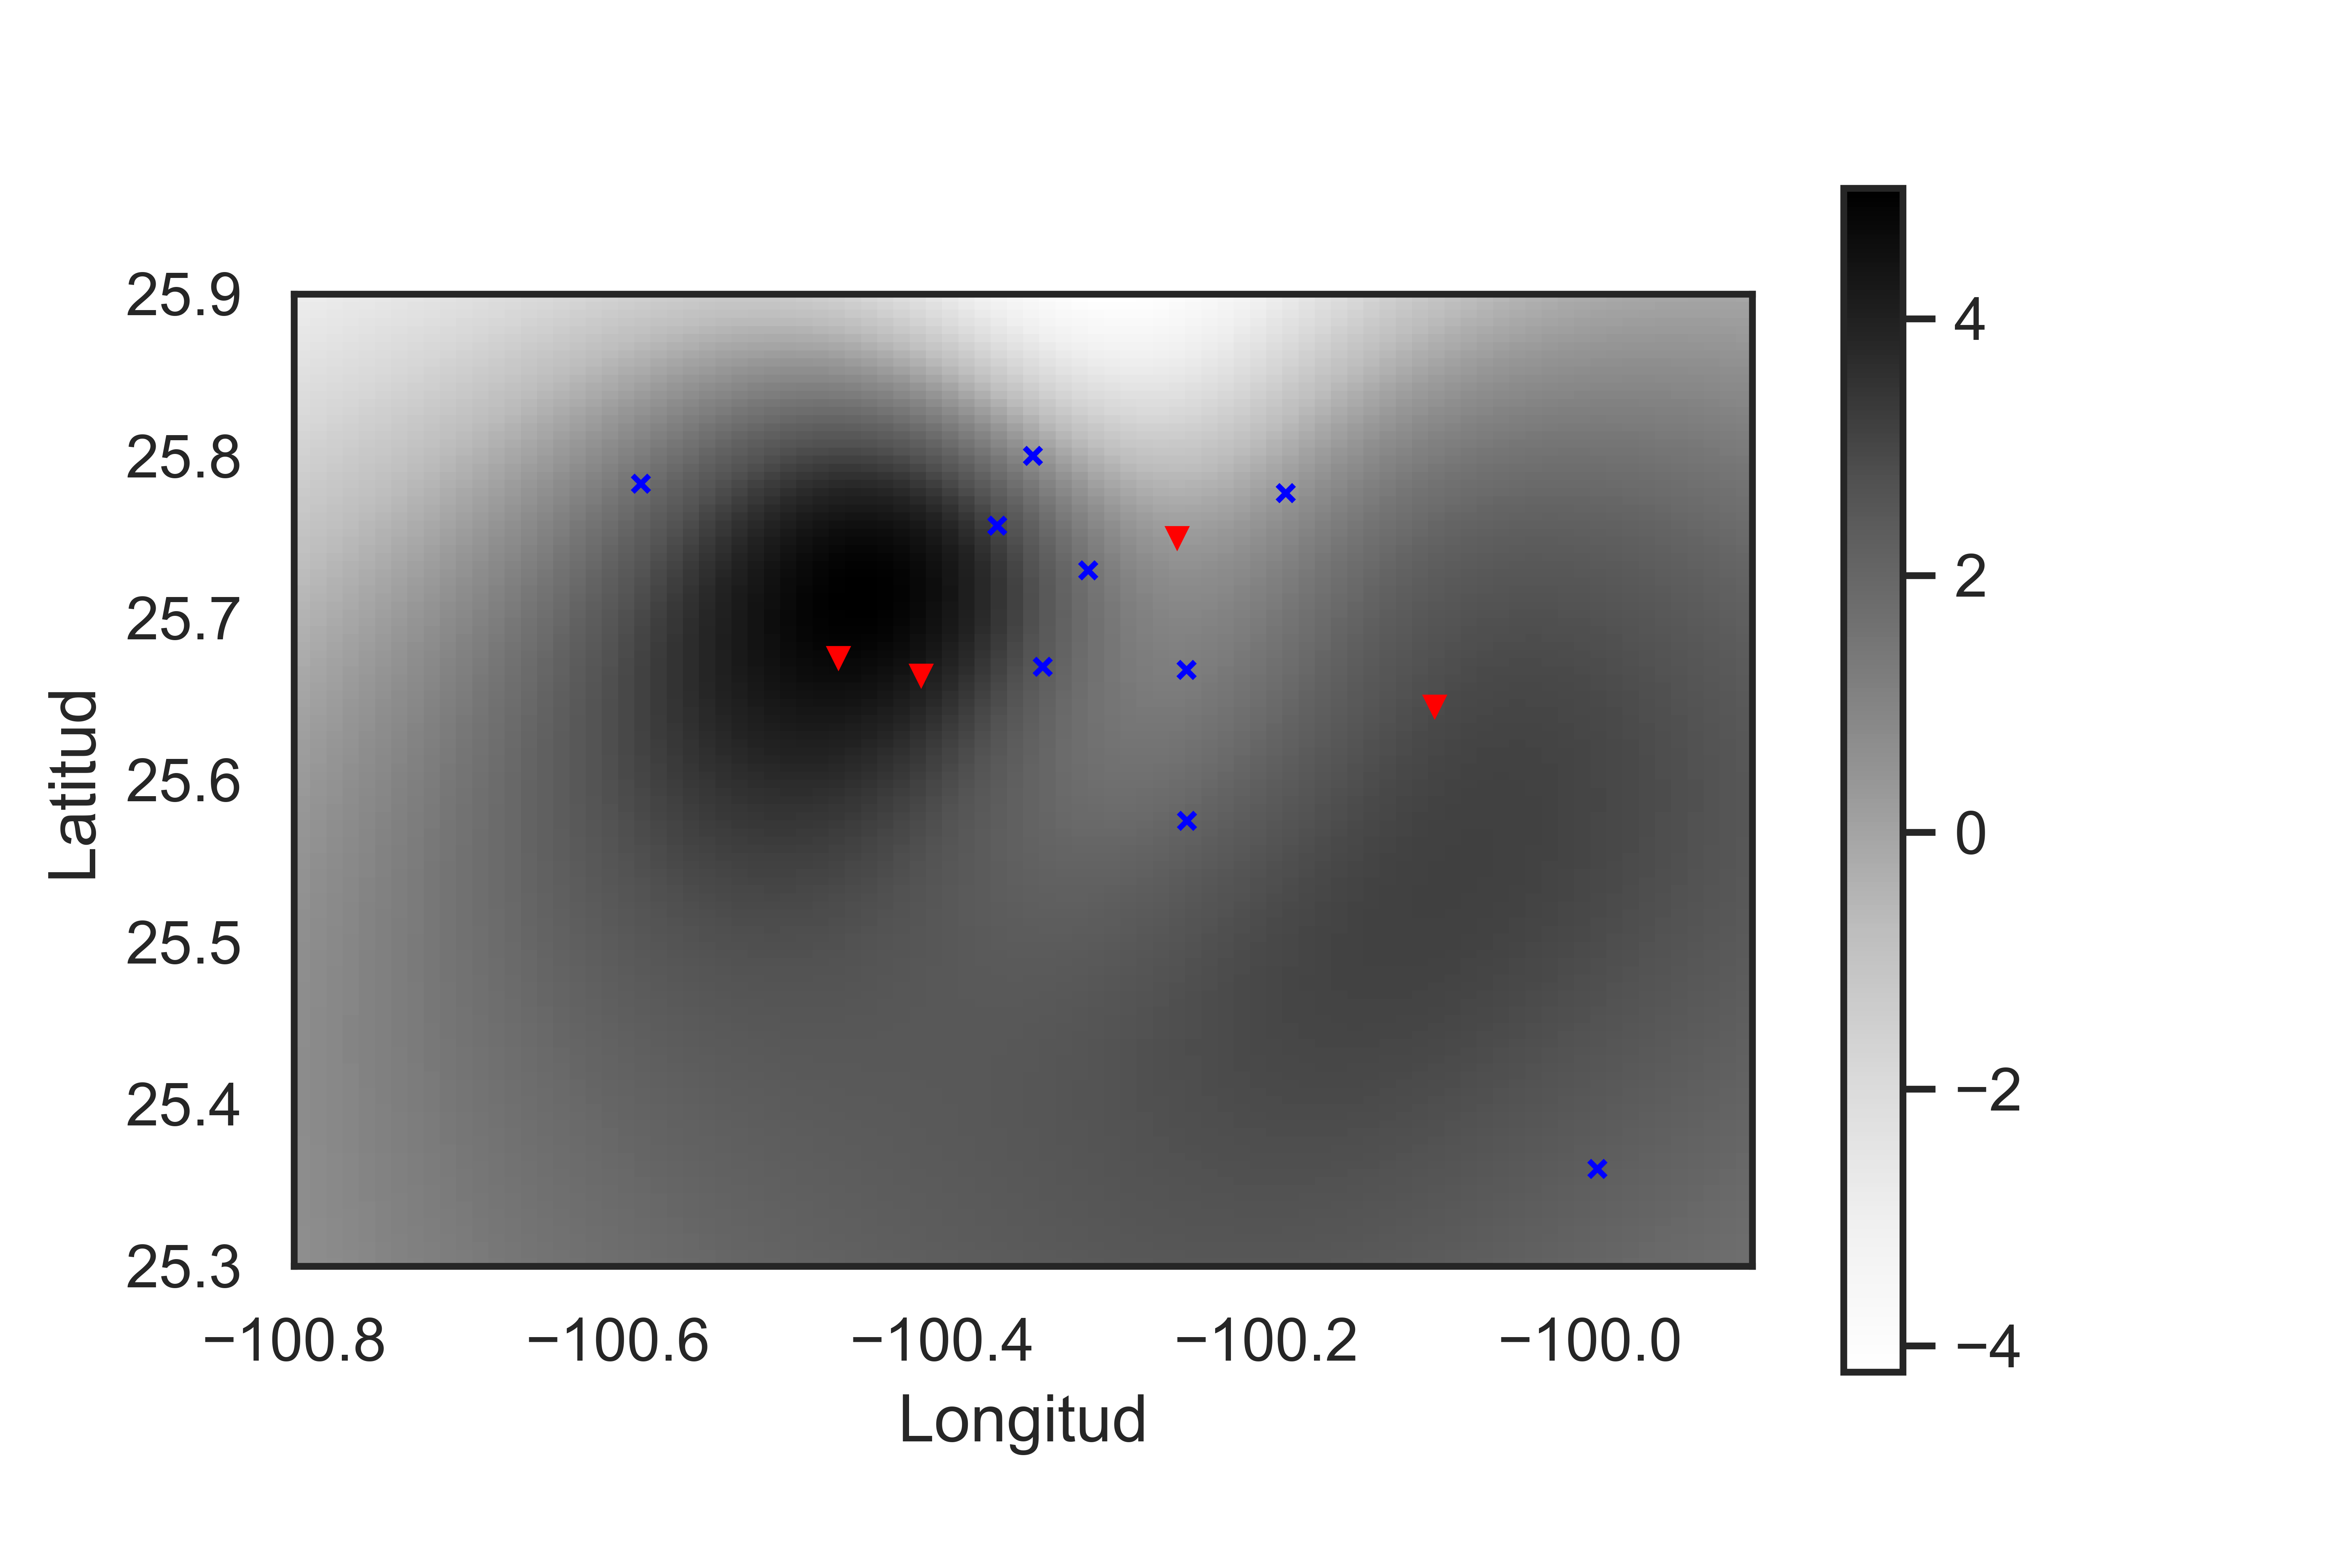
\includegraphics[width=4cm, height=4cm]{./brf_m_9_0_26302}}
\subfigure[FBR I] {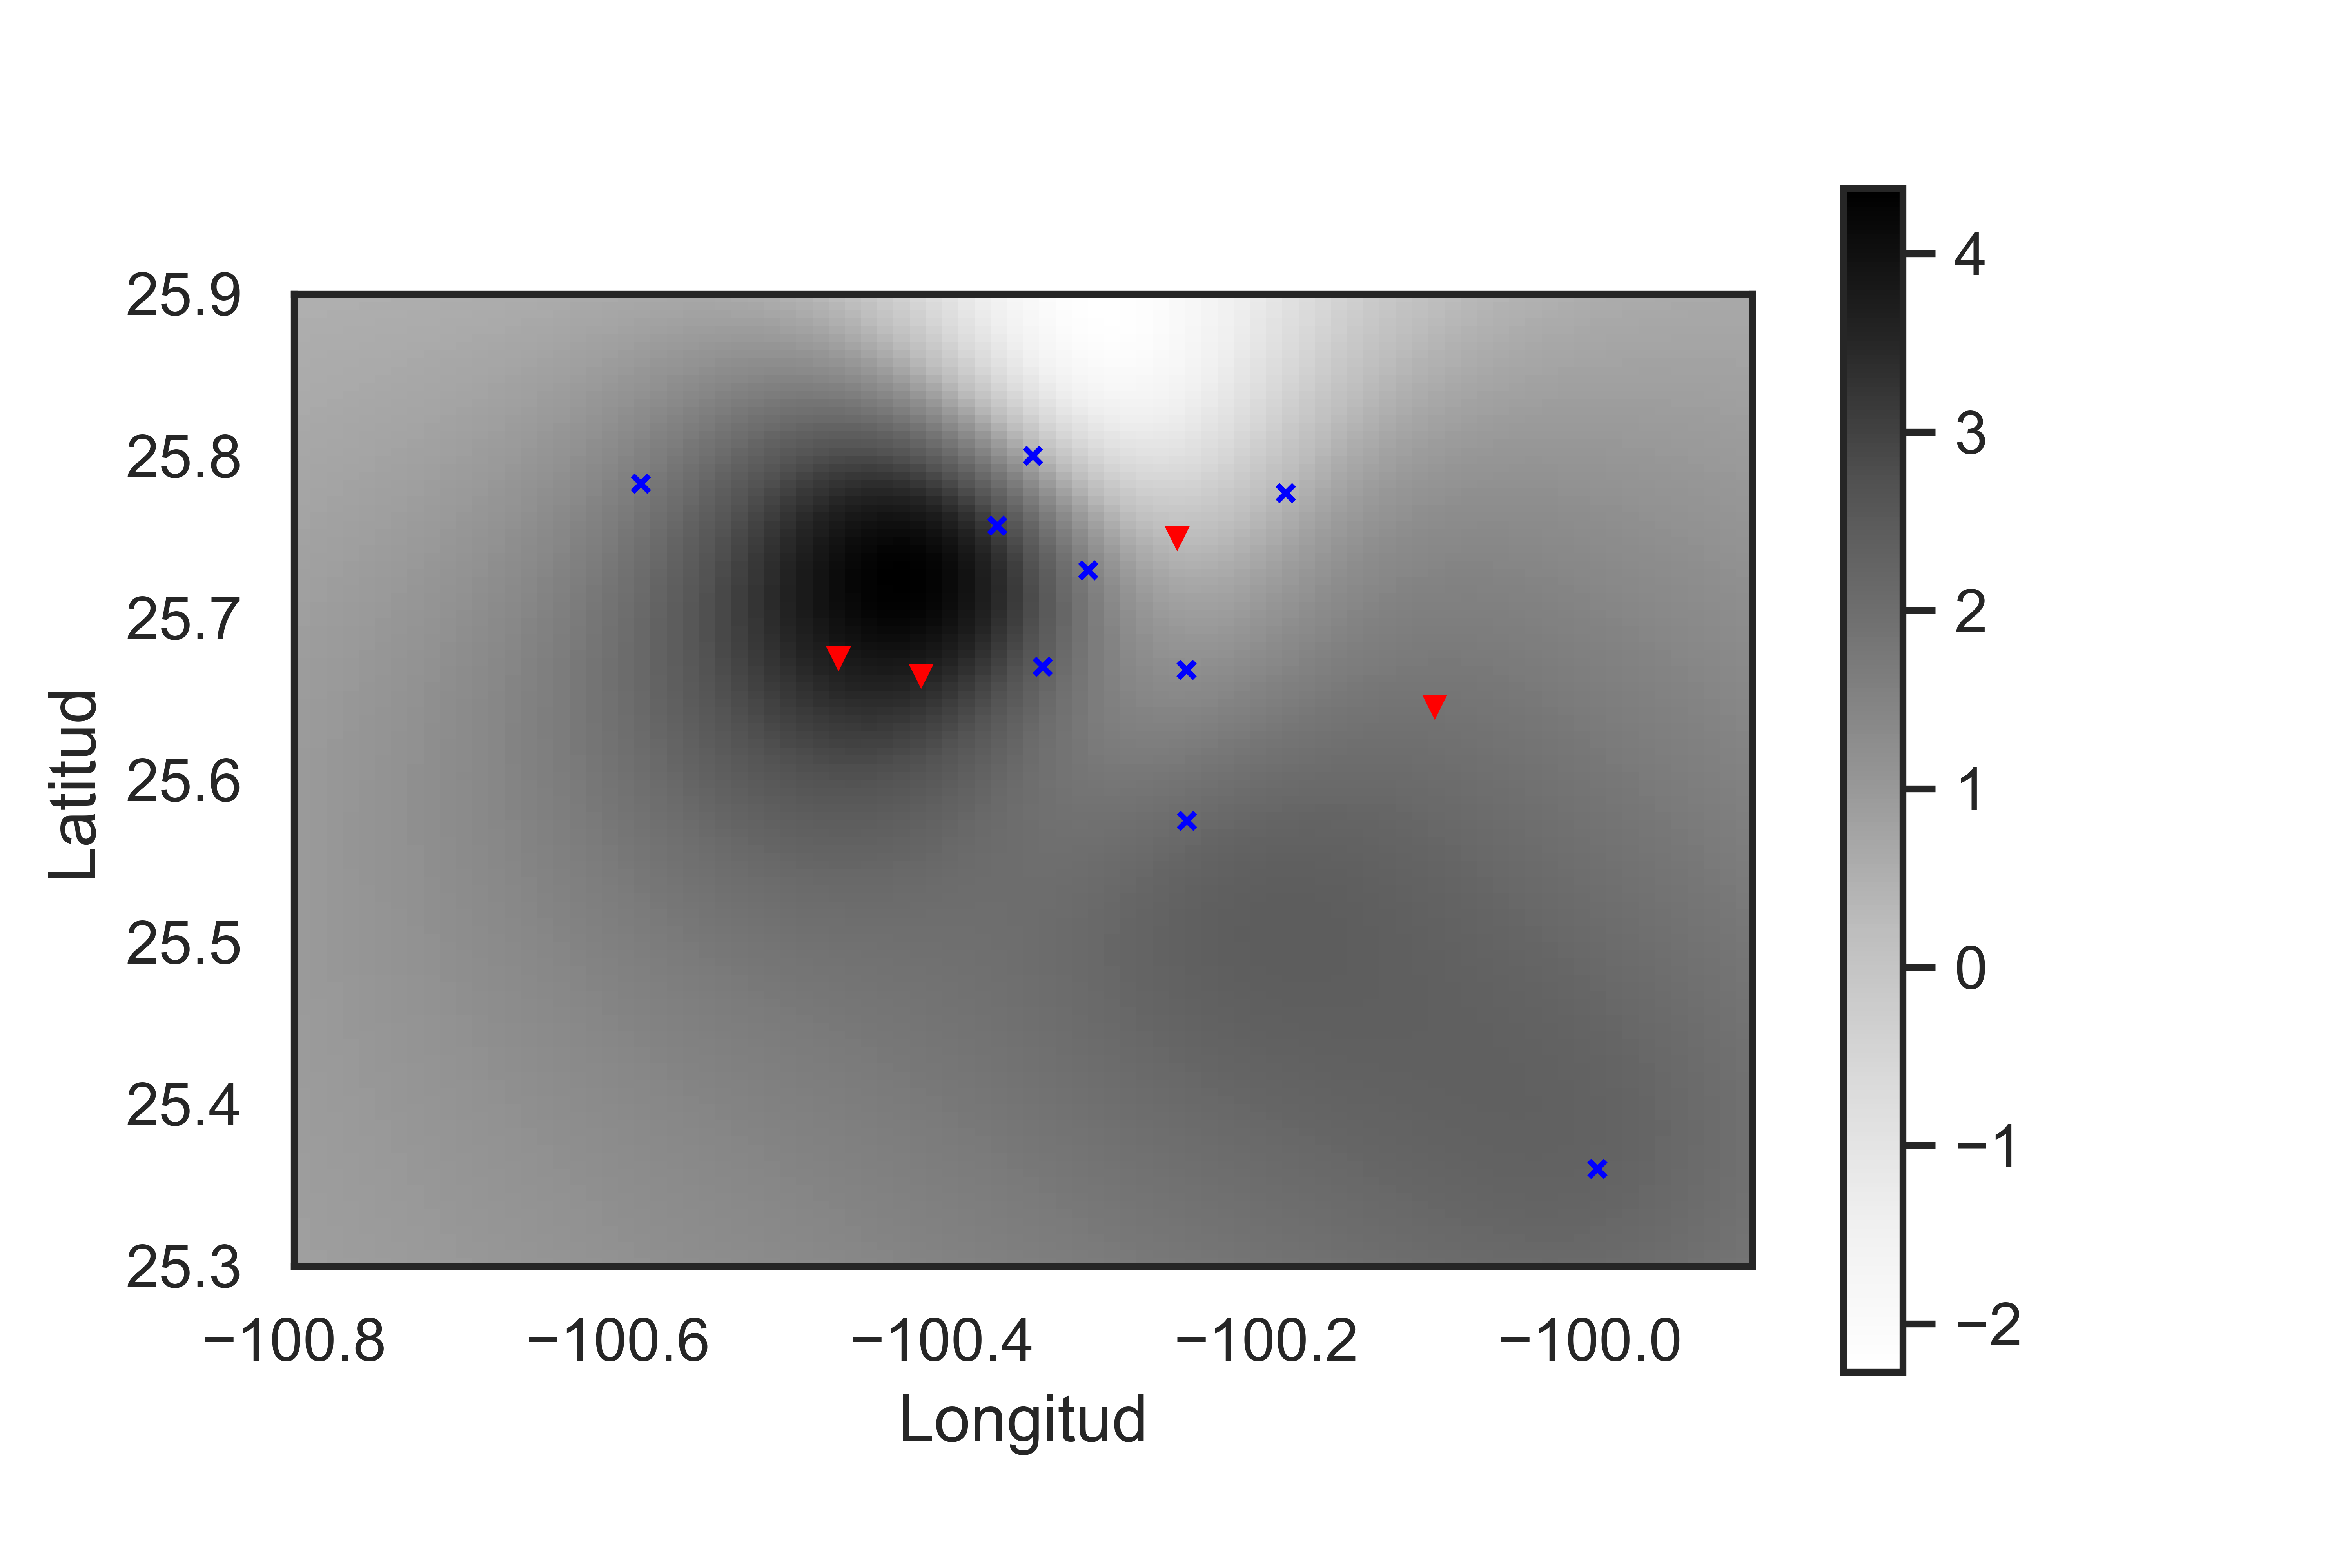
\includegraphics[width=4cm, height=4cm]{./brf_i_9_0_26302}}
\subfigure[FBR G] {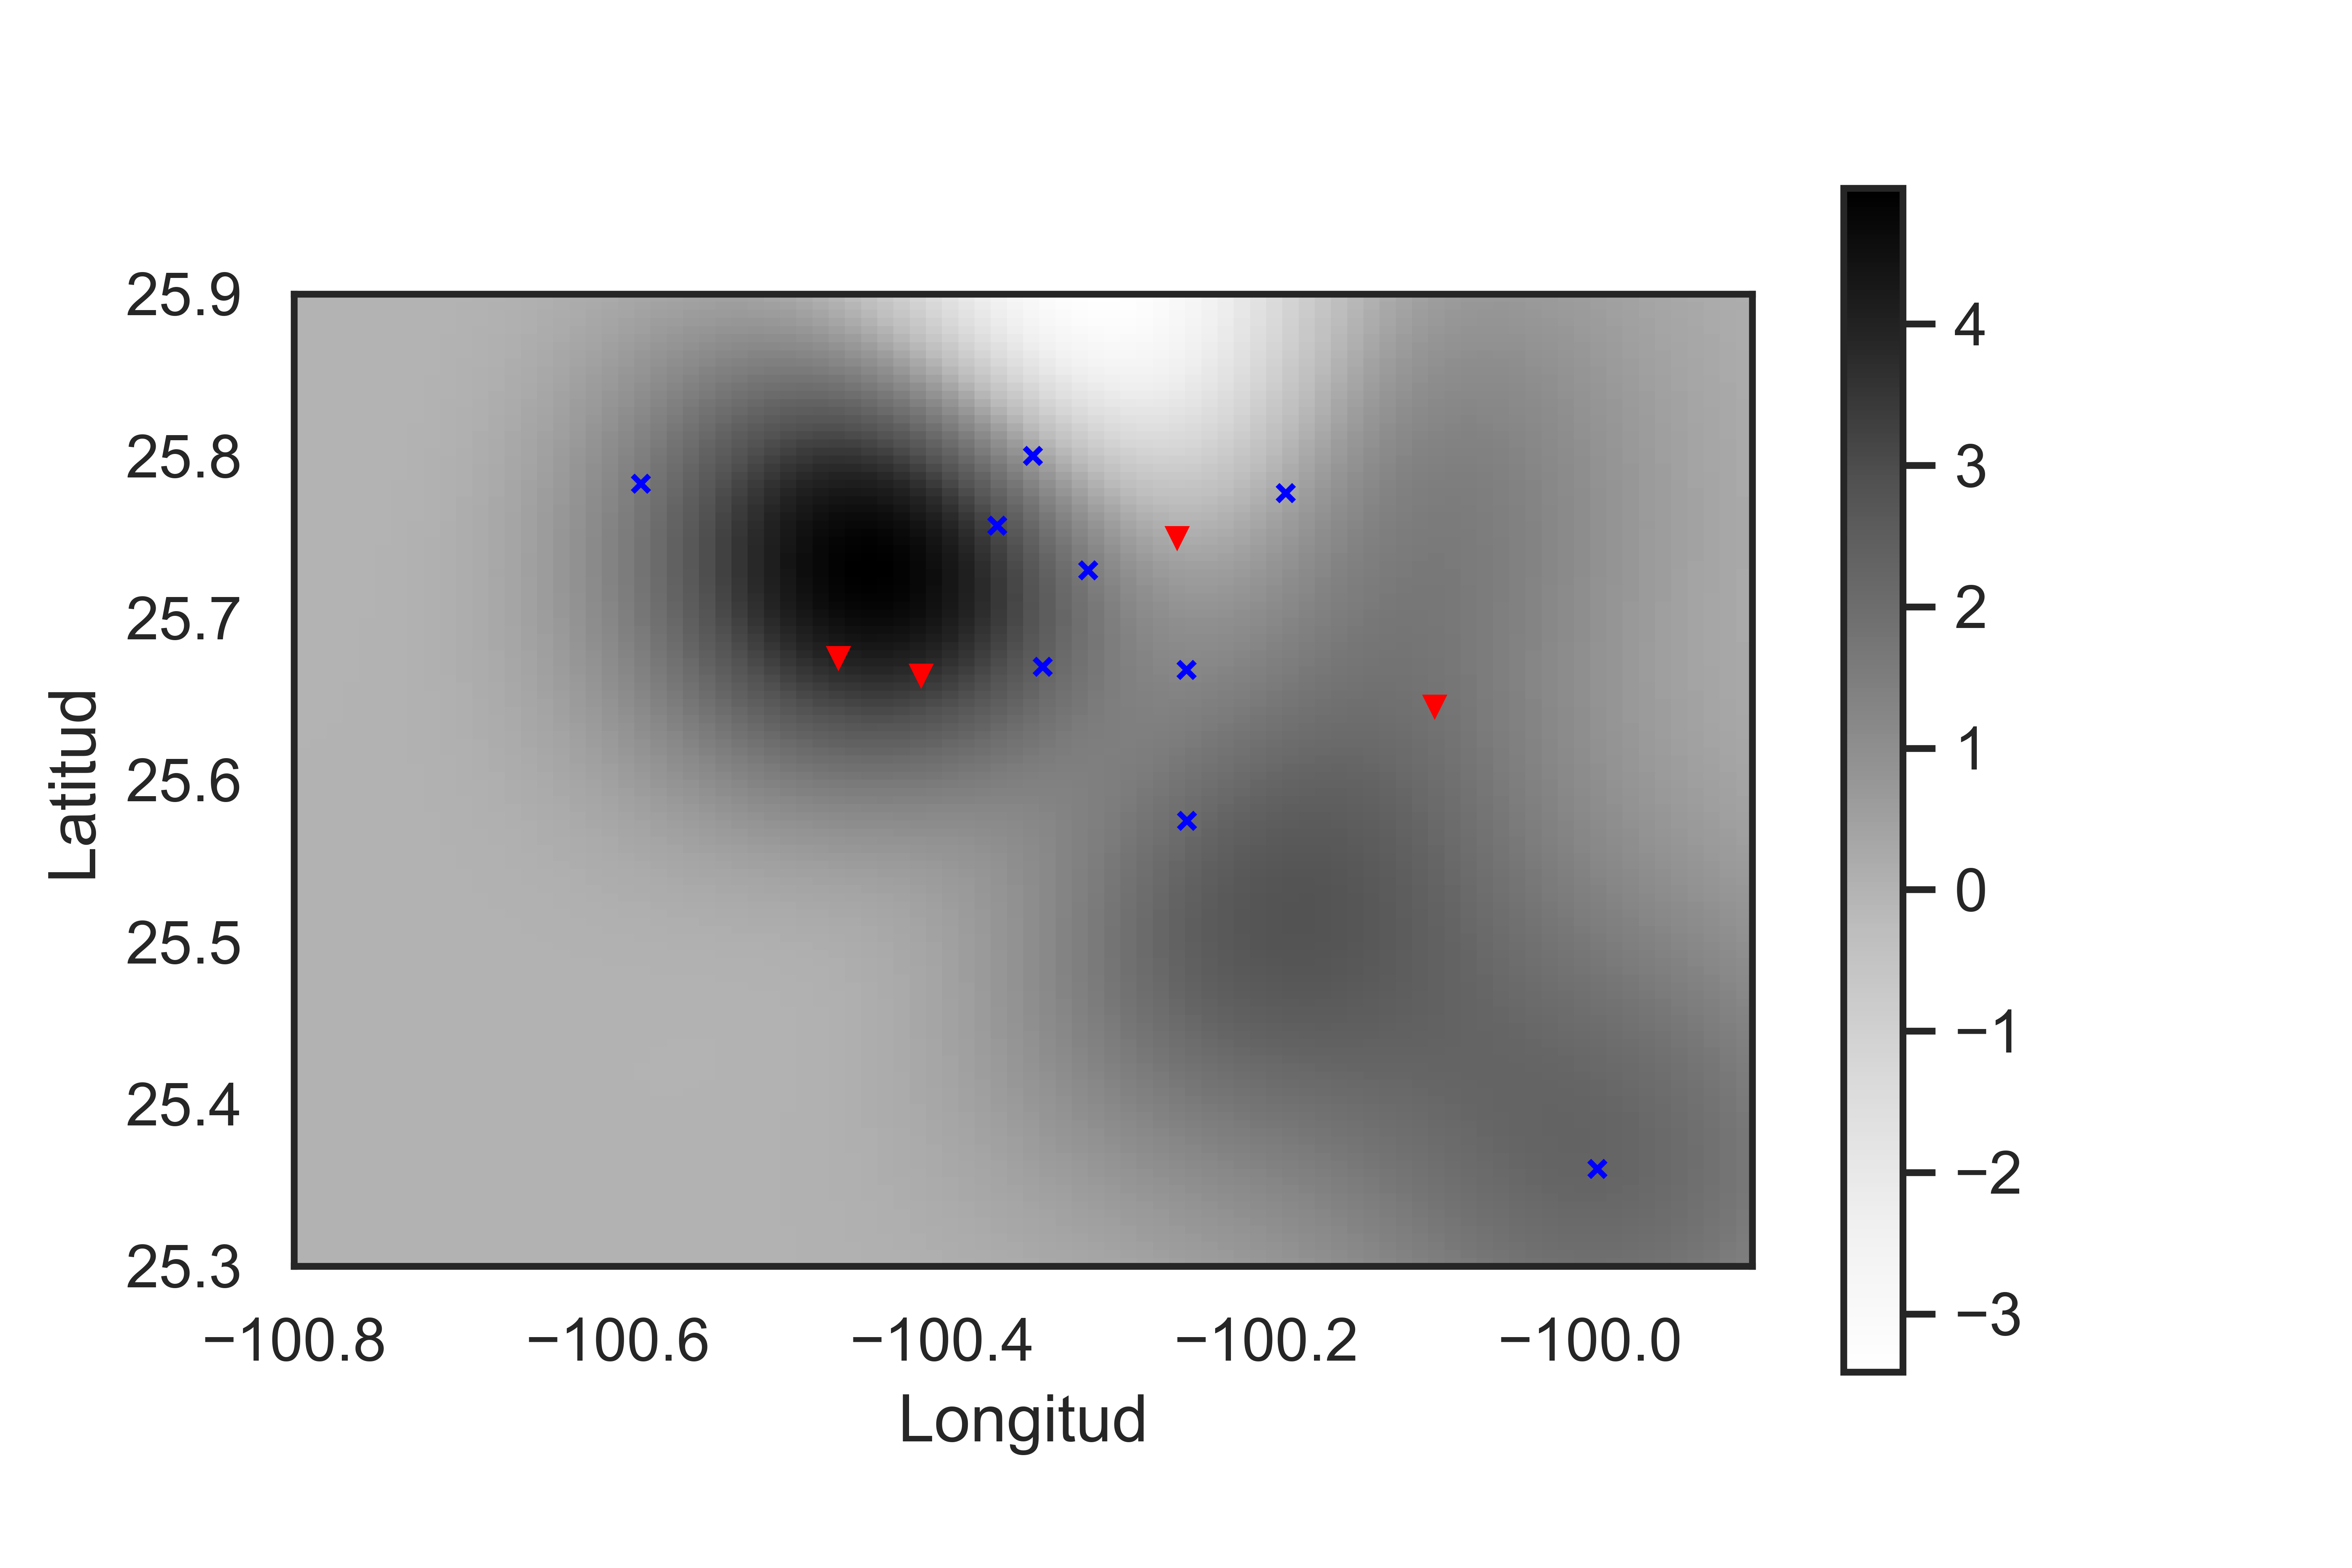
\includegraphics[width=4cm, height=4cm]{./brf_g_9_0_26302}}
\subfigure[FBR L] {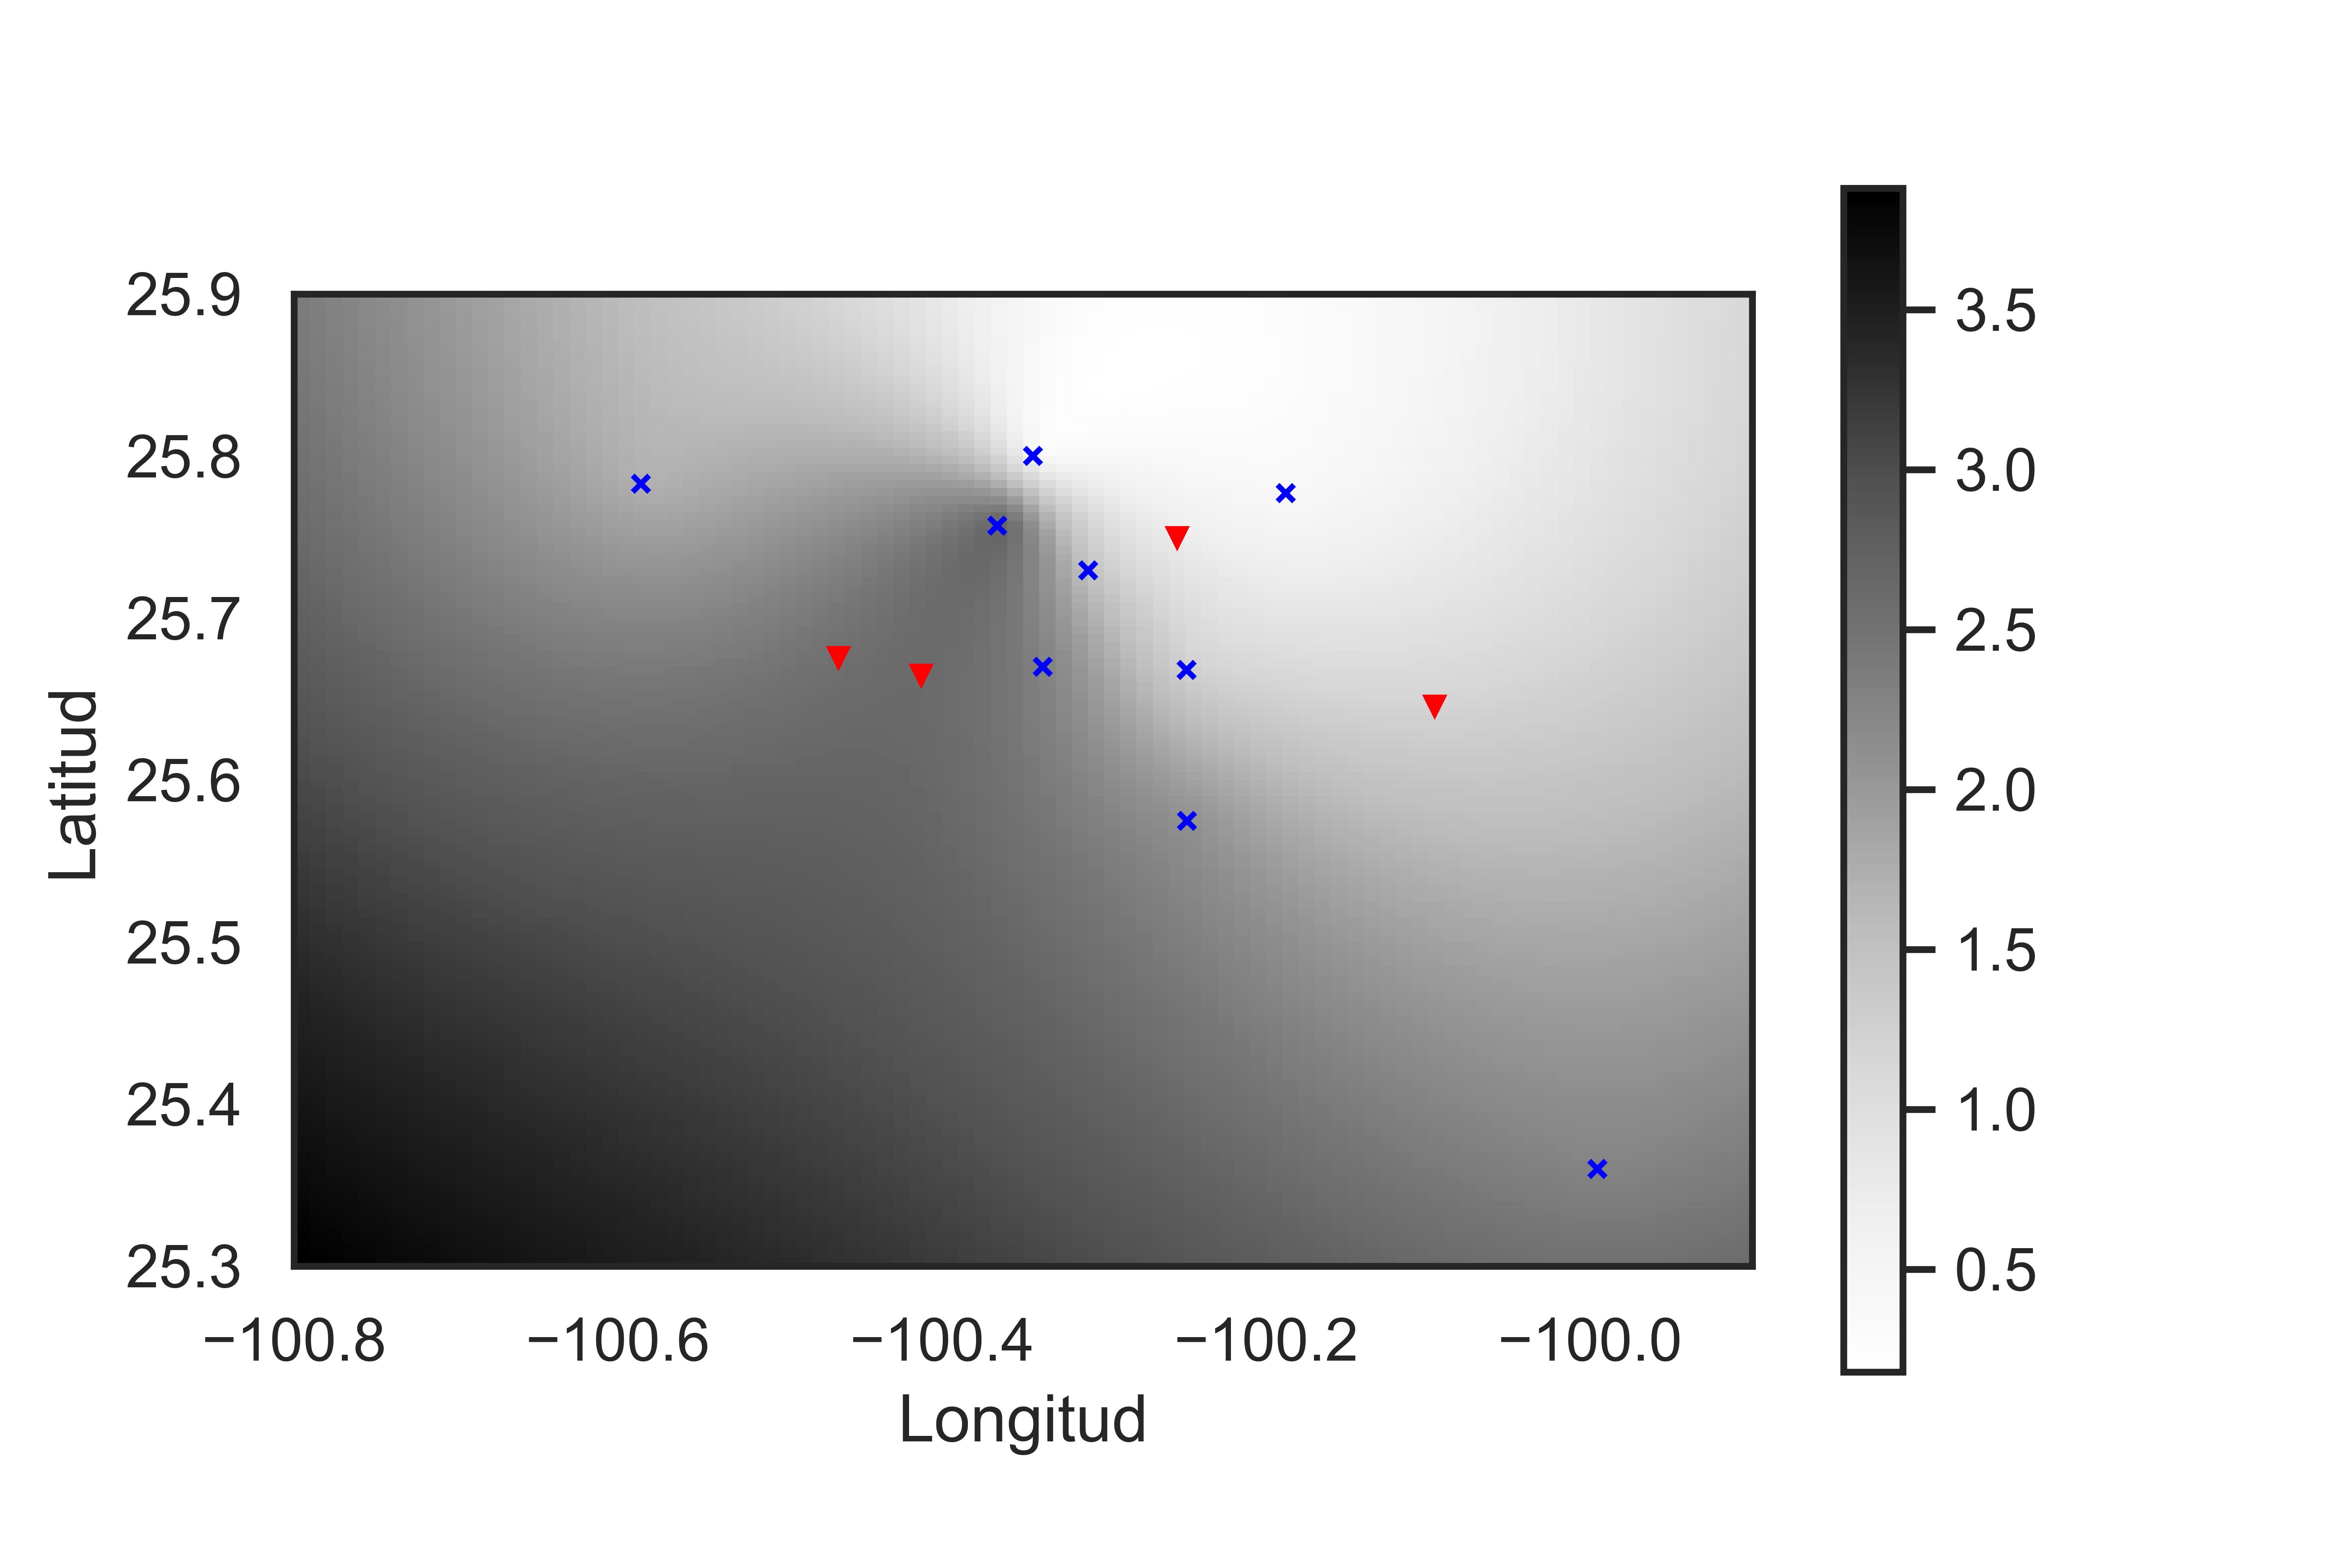
\includegraphics[width=4cm, height=4cm]{./brf_l_9_0_26302}}
\subfigure[FBR C] {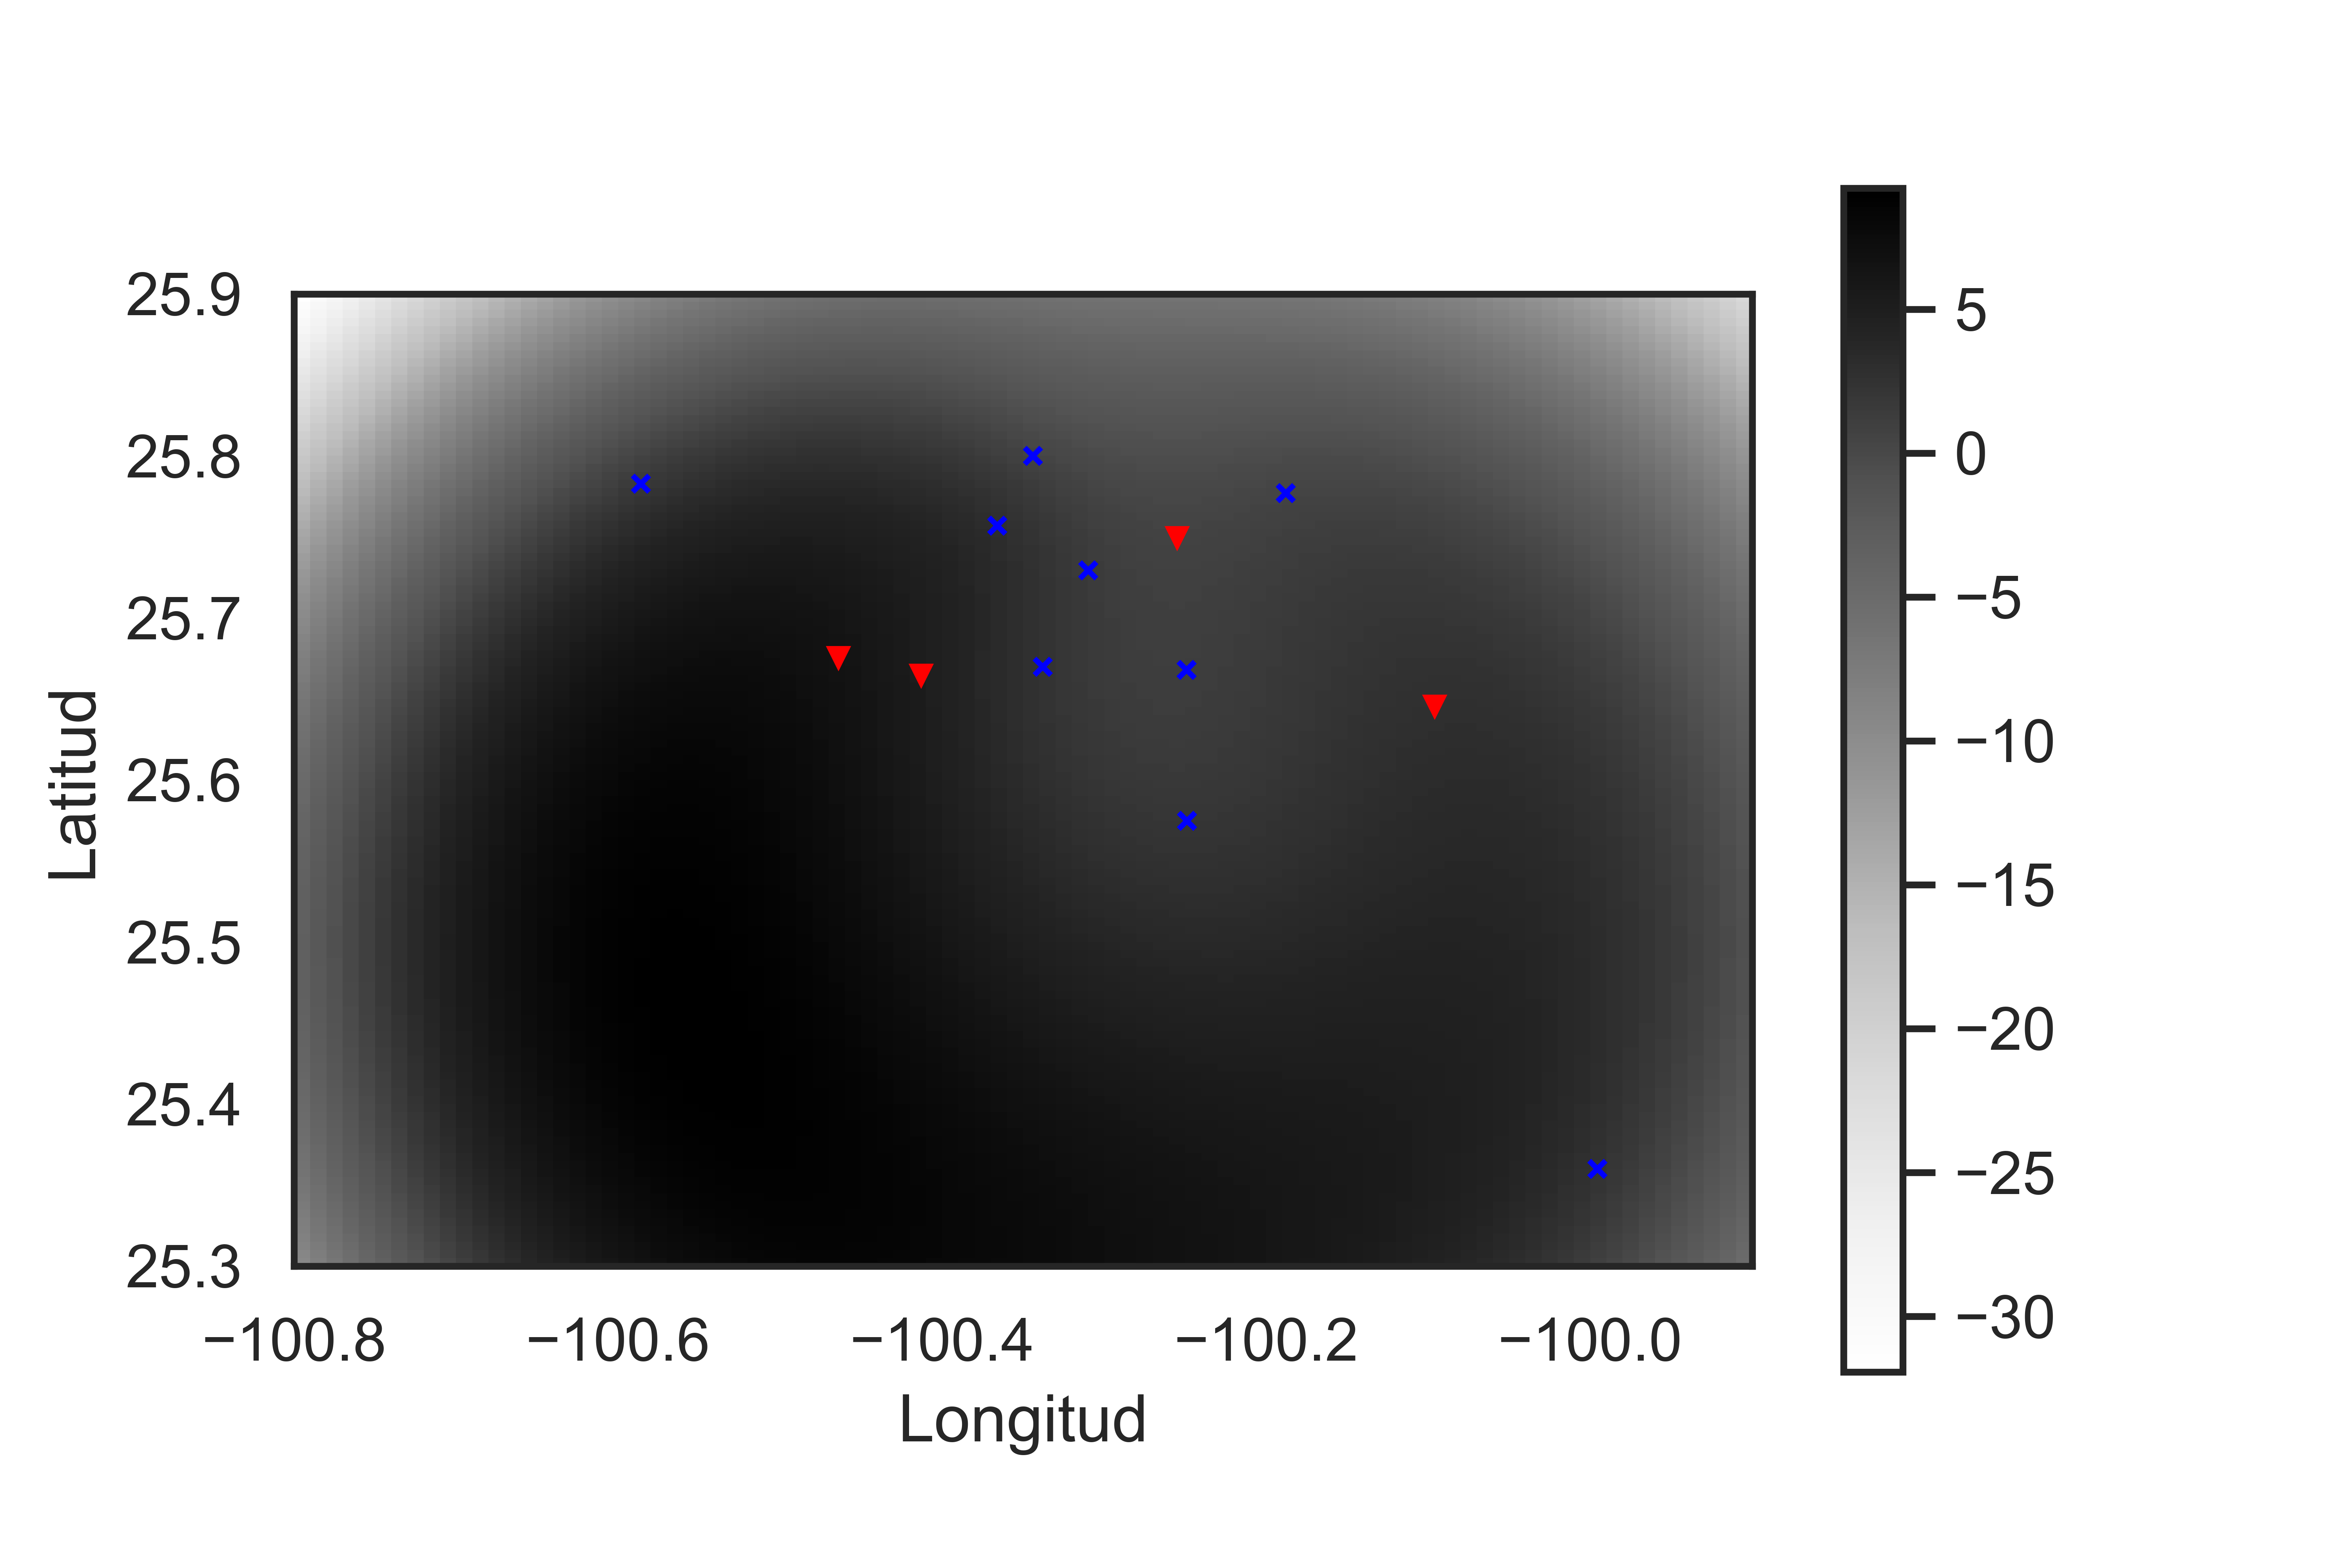
\includegraphics[width=4cm, height=4cm]{./brf_c_9_0_26302}}
\subfigure[FBR Q] {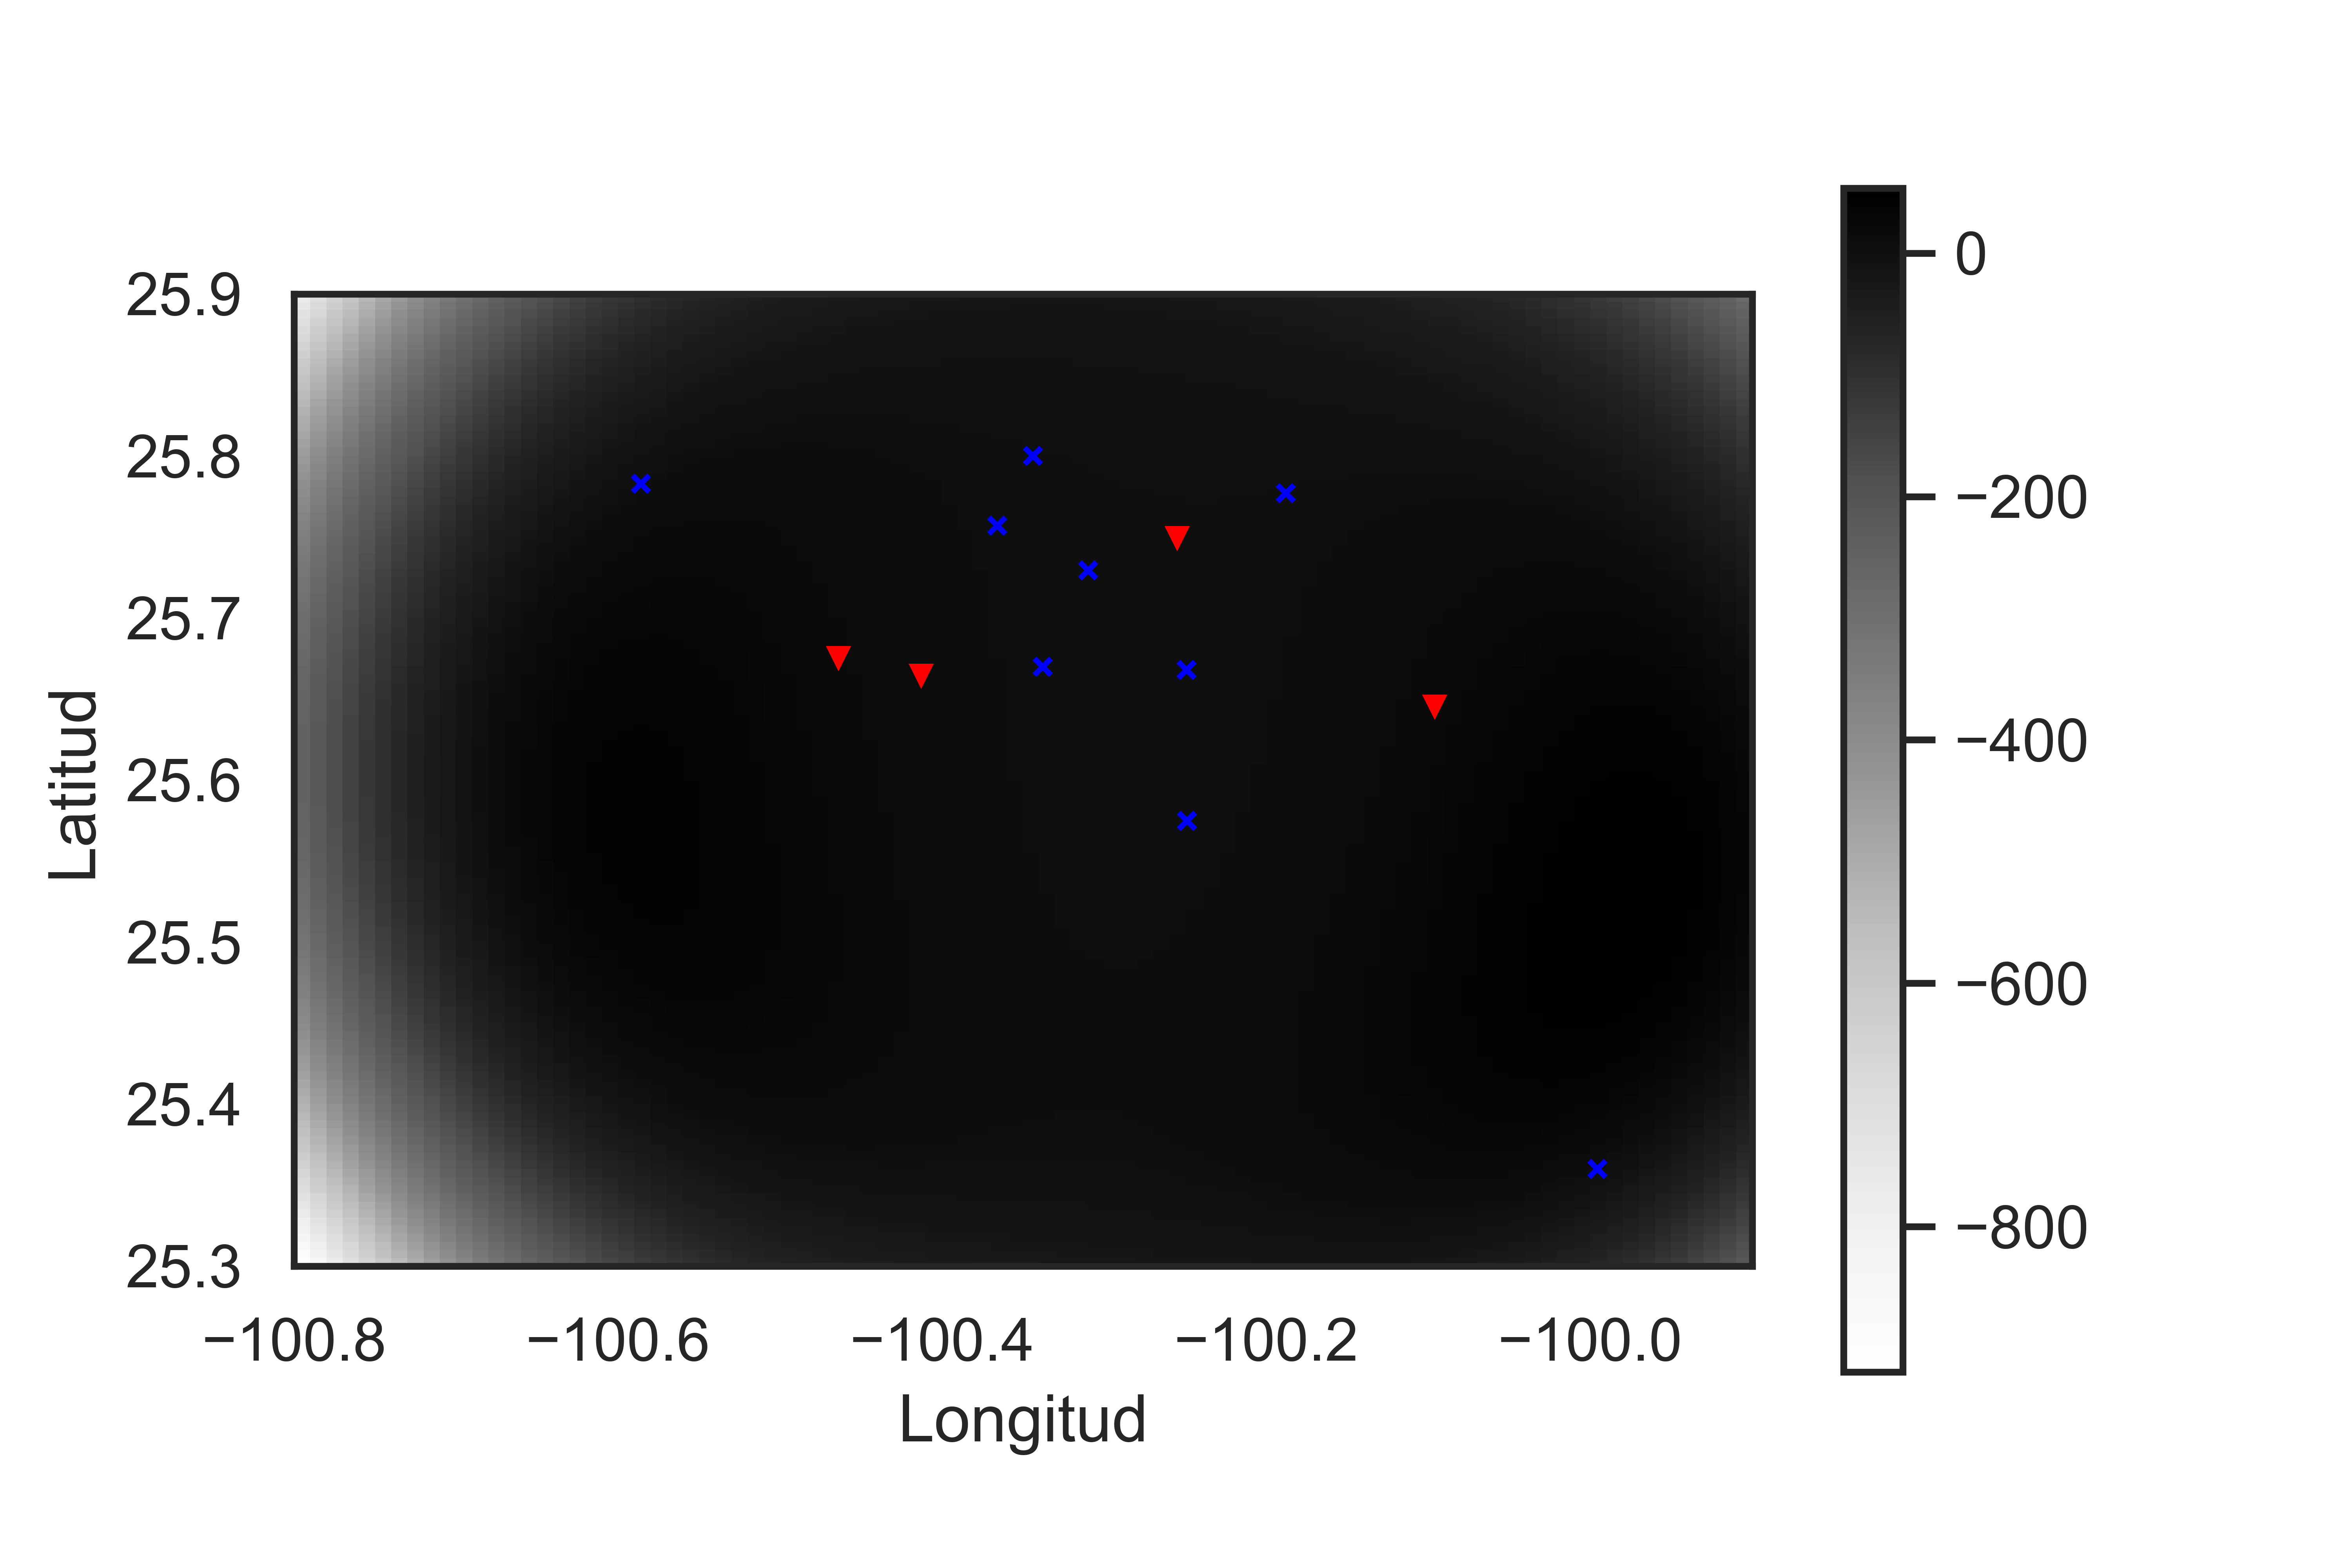
\includegraphics[width=4cm, height=4cm]{./brf_q_9_0_26302}}
\subfigure[FBR TPS] {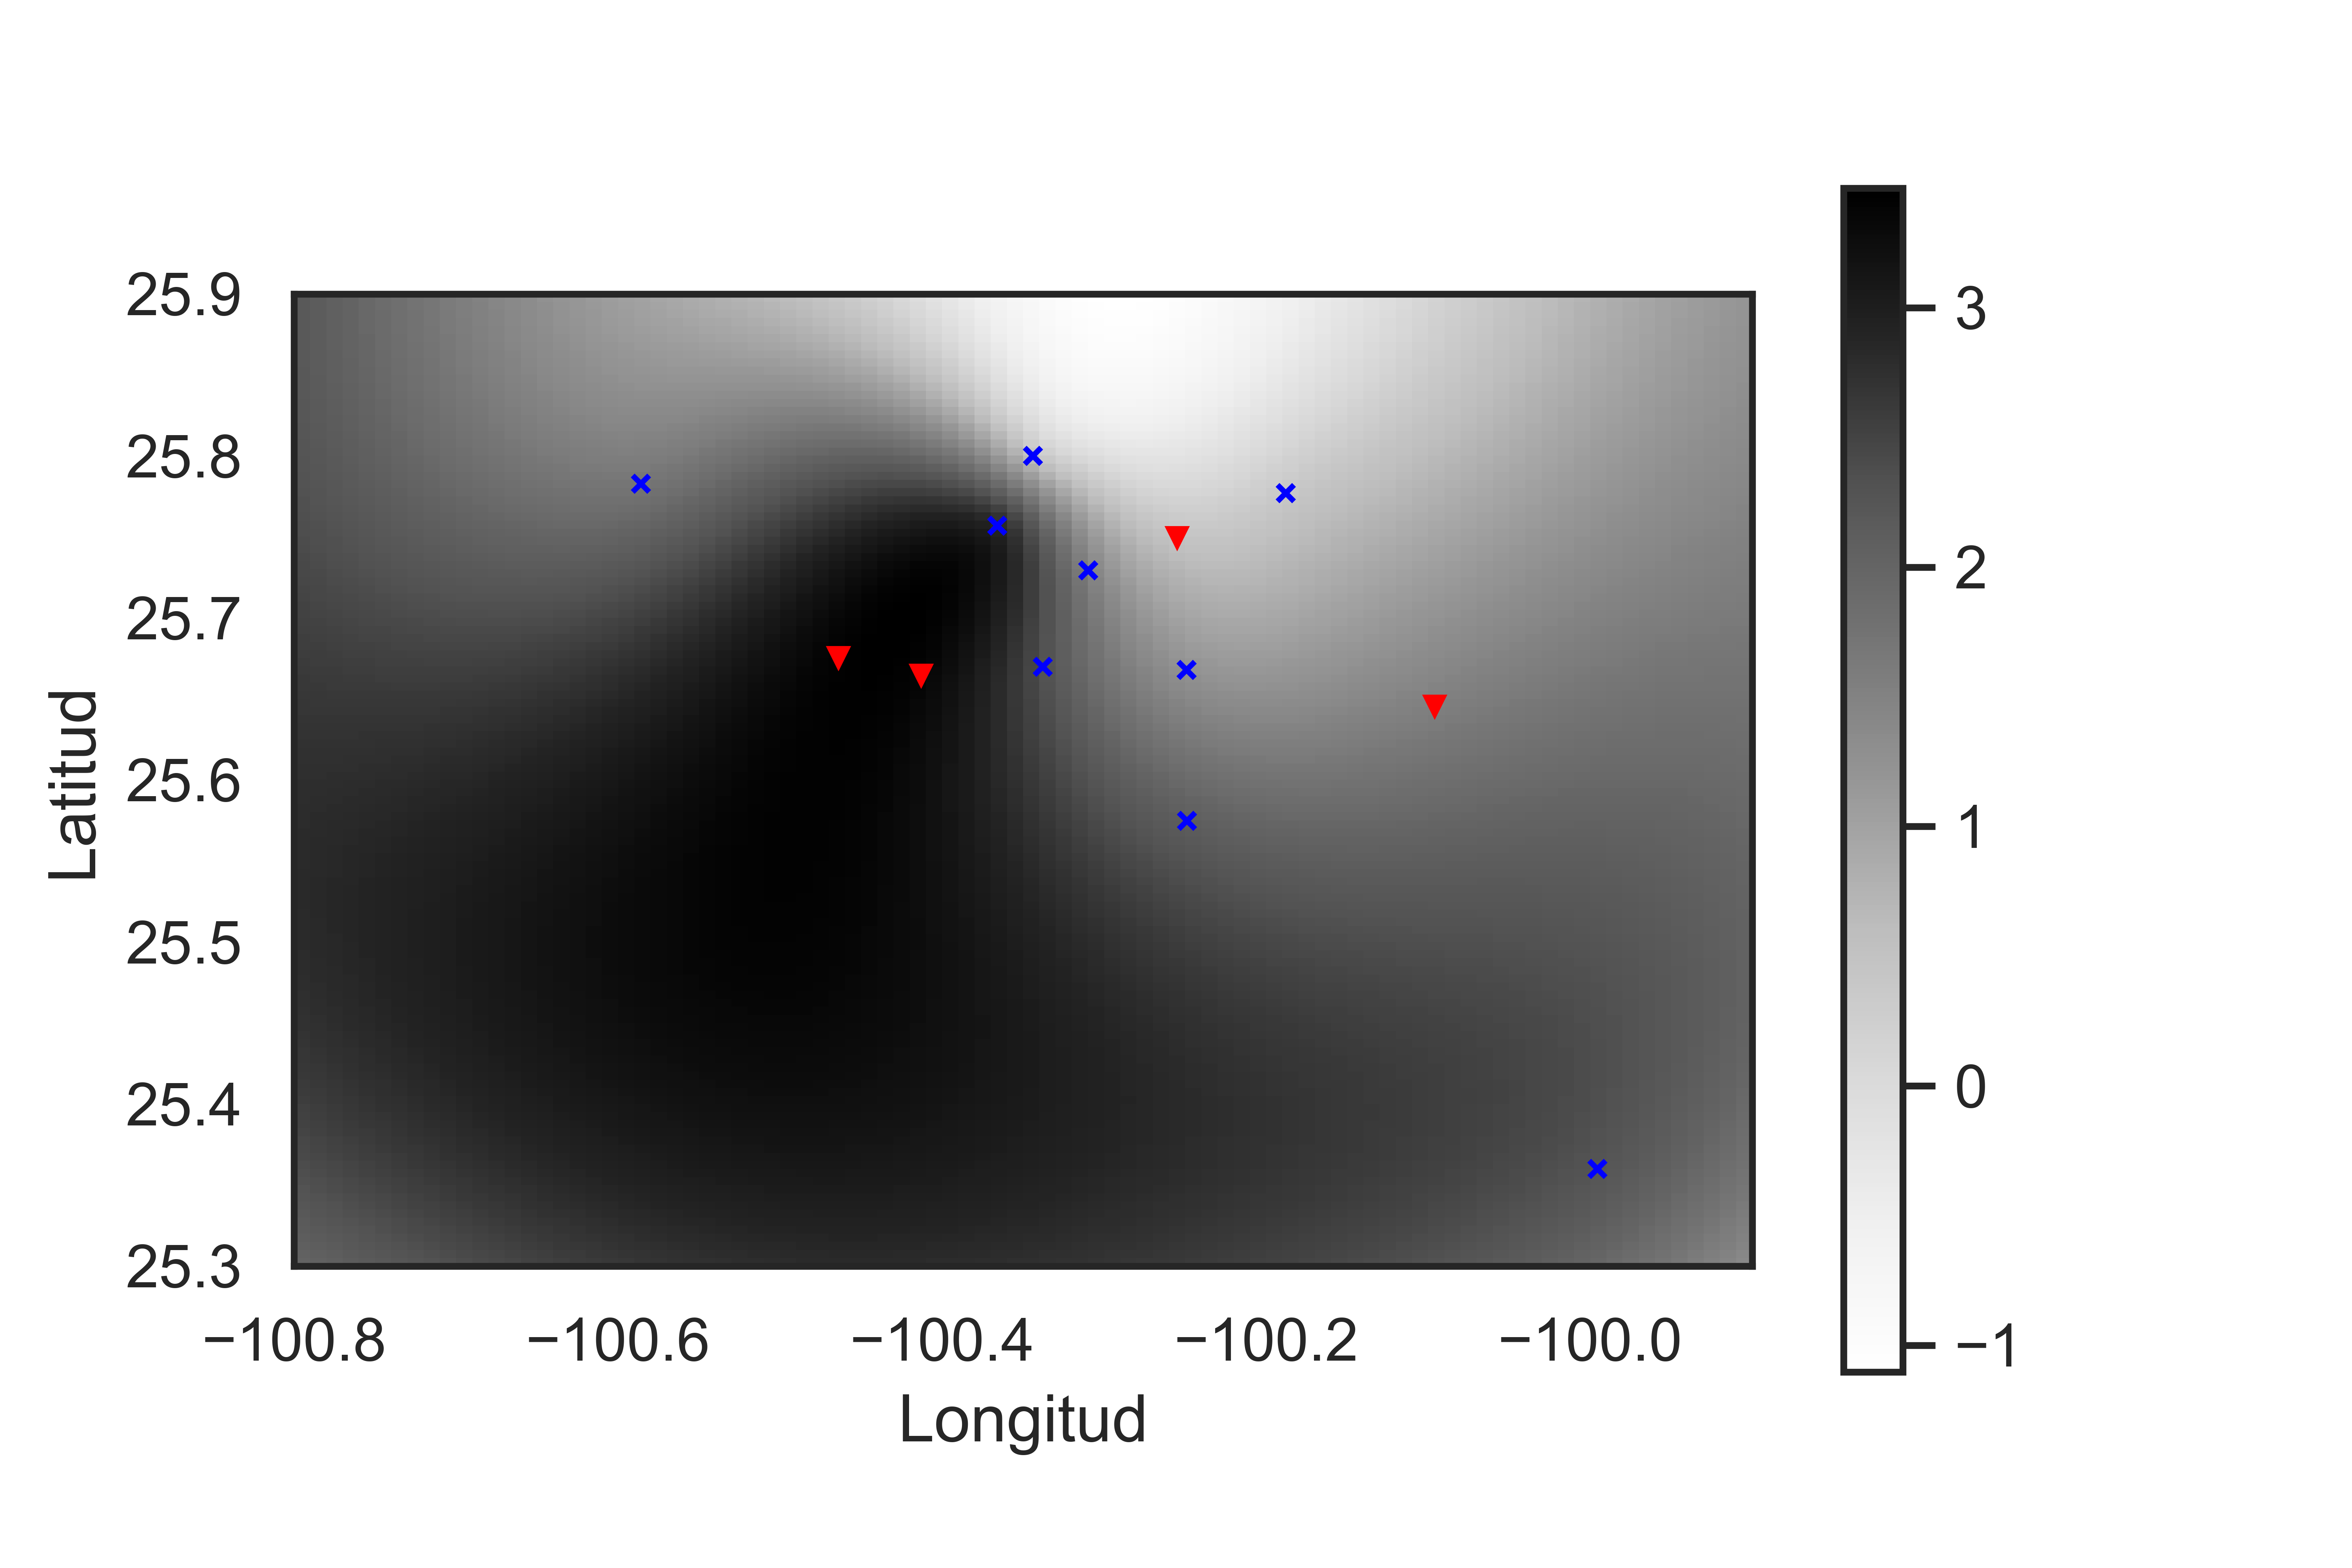
\includegraphics[width=4cm, height=4cm]{./brf_tps_9_0_26302}}
\subfigure[KO] {\includegraphics[width=4cm, height=4cm]{./ok_9_0_26302}}
\subfigure[KU] {\includegraphics[width=4cm, height=4cm]{./uk_9_0_26302}}
\caption{Interpolaciones de CO para 9 estaciones seleccionadas y 4 estaciones interpoladas: Fecha (31-12-2018 23:00:00)}
\label{COfigure1}
\end{figure}

\begin{table}[H]
\centering
\caption{CO: 10 estaciones seleccionadas 3 estaciones interpoladas}
\begin{adjustbox}{max width=0.9\textwidth}
\begin{tabular}{|c|c|c|c|c|c|c|}
\hline
\multicolumn{7}{ |c| }{Métricas de error} \\ \hline
Método &MAPE &MAE &MAEP &RMSE &RMSEP &MSE \\ \hline
TV &1.064 &0.94 &0.71 &1.24 &0.93 &1.55 \\
DIP &0.88 &0.88 &0.66 &1.11 &0.84 &1.25 \\
FBR M &$1.35\times10^{17}$ &$1.88\times10^{17}$ &$1.41\times10^{17}$ &$1.31\times10^{18}$ &$9.92\times10^{17}$ &$1.73\times10^{36}$ \\
FBR IM &$6.25\times10^{13}$ &$1.16\times10^{14}$ &$8.79\times10^{13}$ &$3.28\times10^{16}$ &$2.47\times10^{16}$ &$1.07\times10^{33}$ \\
FBR G &$9.04\times10^{15}$ &$8.88\times10^{15}$ &$6.68\times10^{15}$ &$2.86\times10^{17}$ &$2.15\times10^{17}$ &$8.19\times10^{34}$ \\
FBR L &1.09 &1.00 &0.75 &1.32 &0.99 &1.75 \\
FBR C &$6.38\times10^{17}$ &$6.06\times10^{17}$ &$4.56\times10^{17}$ &$2.36\times10^{18}$ &$1.77\times10^{18}$ &$5.59\times10^{36}$ \\
FBR Q &$2.80\times10^{18}$ &$1.94\times10^{18}$ &$1.46\times10^{18}$ &$4.23\times10^{18}$ &$3.18\times10^{18}$ &$1.79\times10^{37}$ \\
FBR TPS &$1.90\times10^{15}$ &$2.10\times10^{15}$ &$1.58\times10^{14}$ &$1.39\times10^{17}$ &$1.04\times10^{17}$ &$1.94\times10^{34}$ \\
KO &0.87 &0.88 &0.66 &1.11 &0.83 &1.23 \\
KU &1.14 &1.00 &0.75 &1.41 &1.06 &1.99 \\\hline
\end{tabular}
\end{adjustbox}
\label{tabCO_2}
\end{table}

De la tabla \ref{tabCO_2}, en la cual se utilizan diez estaciones para interpolar otras tres, podemos ver que los métodos que obtienen peores resultados de predicción son los métodos de Funciones de Base Radial, a excepción del método lineal (FBR L). Entre los métodos deterministas, el DIP obtuvo el menor MAPE, MAE, MAEP, RMSE, RMSEP y MSE, mientras que de los métodos geoestadísticos el método KO obtuvo el menor MAPE, MAE, MAEP, RMSE, RMSEP y MSE; en general DIP y KO son mejores que el resto de los métodos pero KO es mejor que DIP, ya que obtube resultados menores en los errores MAPE, RMSEP y MSE, mientras que en el resto fueron iguales a los errores de DIP. En la figura \ref{COfigure2}, se pueden observar las interpolaciones de cada método, donde las puntos azules son las estaciones seleccionadas y los puntos rojos son las estaciones interpoladas.

\begin{figure}[H]
\centering
\subfigure[TV] {\includegraphics[width=4cm, height=4cm]{./voronoi_10_0_26302}}
\subfigure[DIP] {\includegraphics[width=4cm, height=4cm]{./idw_10_0_26302}}
\subfigure[FBR M] {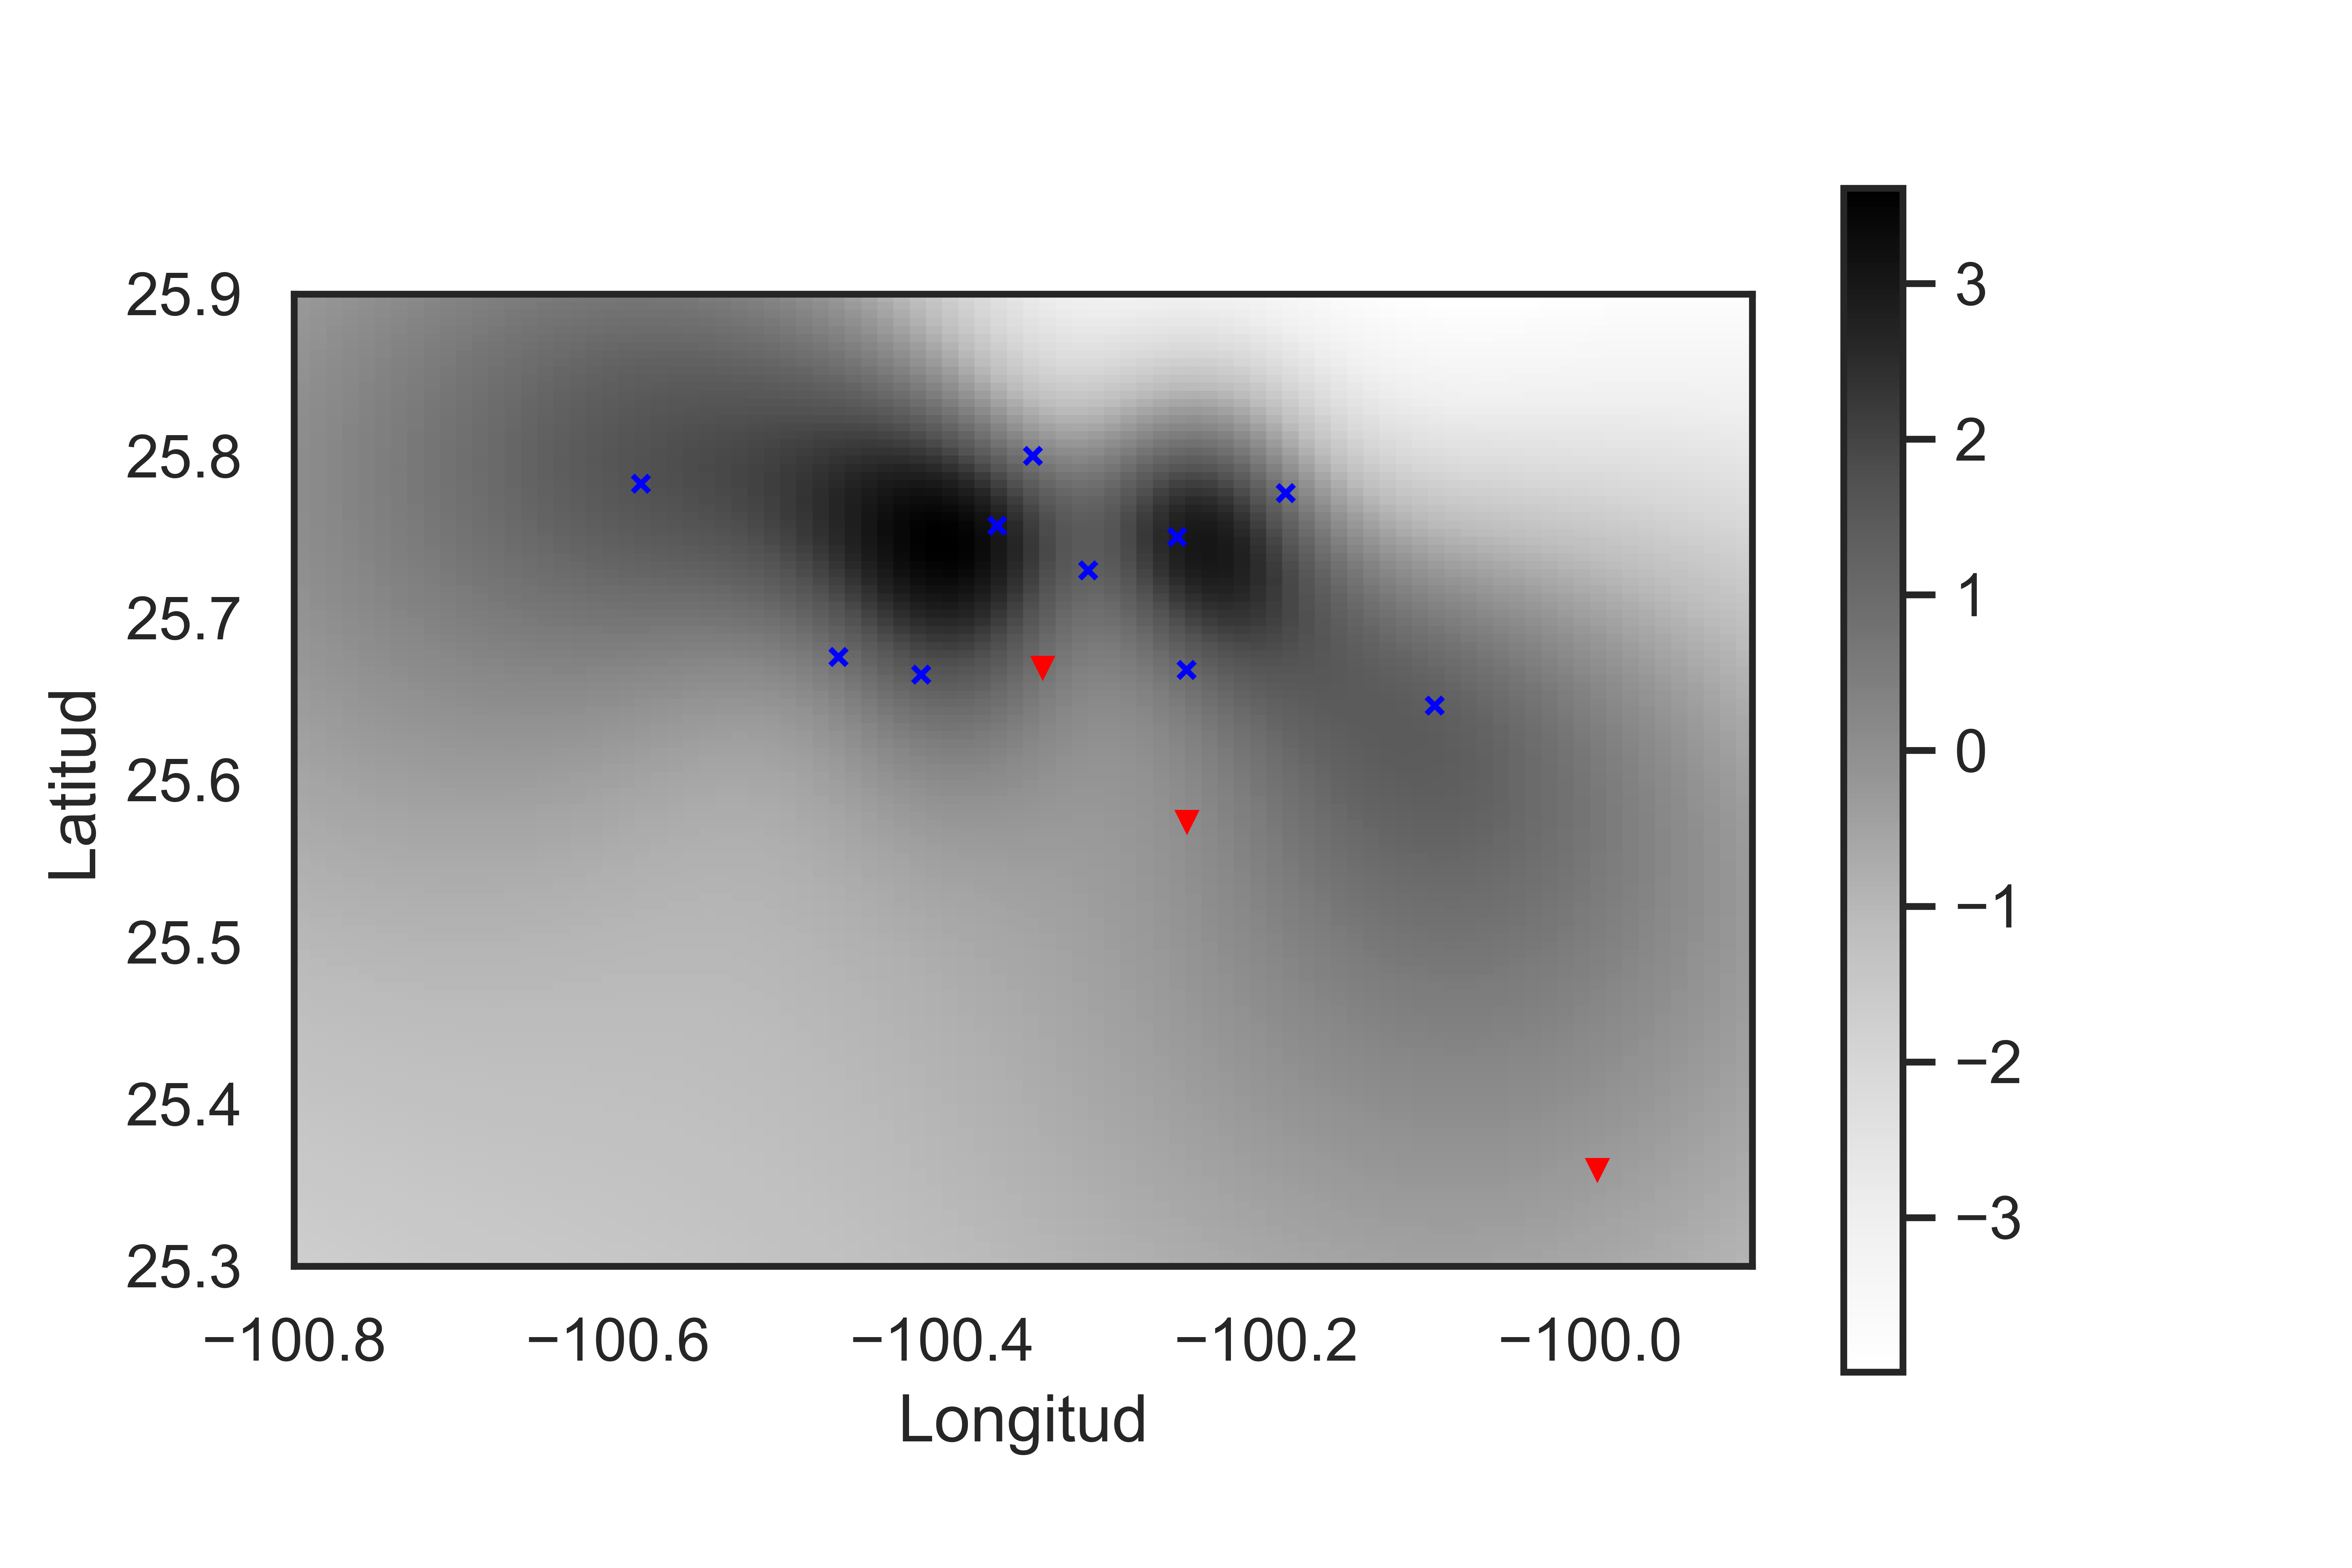
\includegraphics[width=4cm, height=4cm]{./brf_m_10_0_26302}}
\subfigure[FBR I] {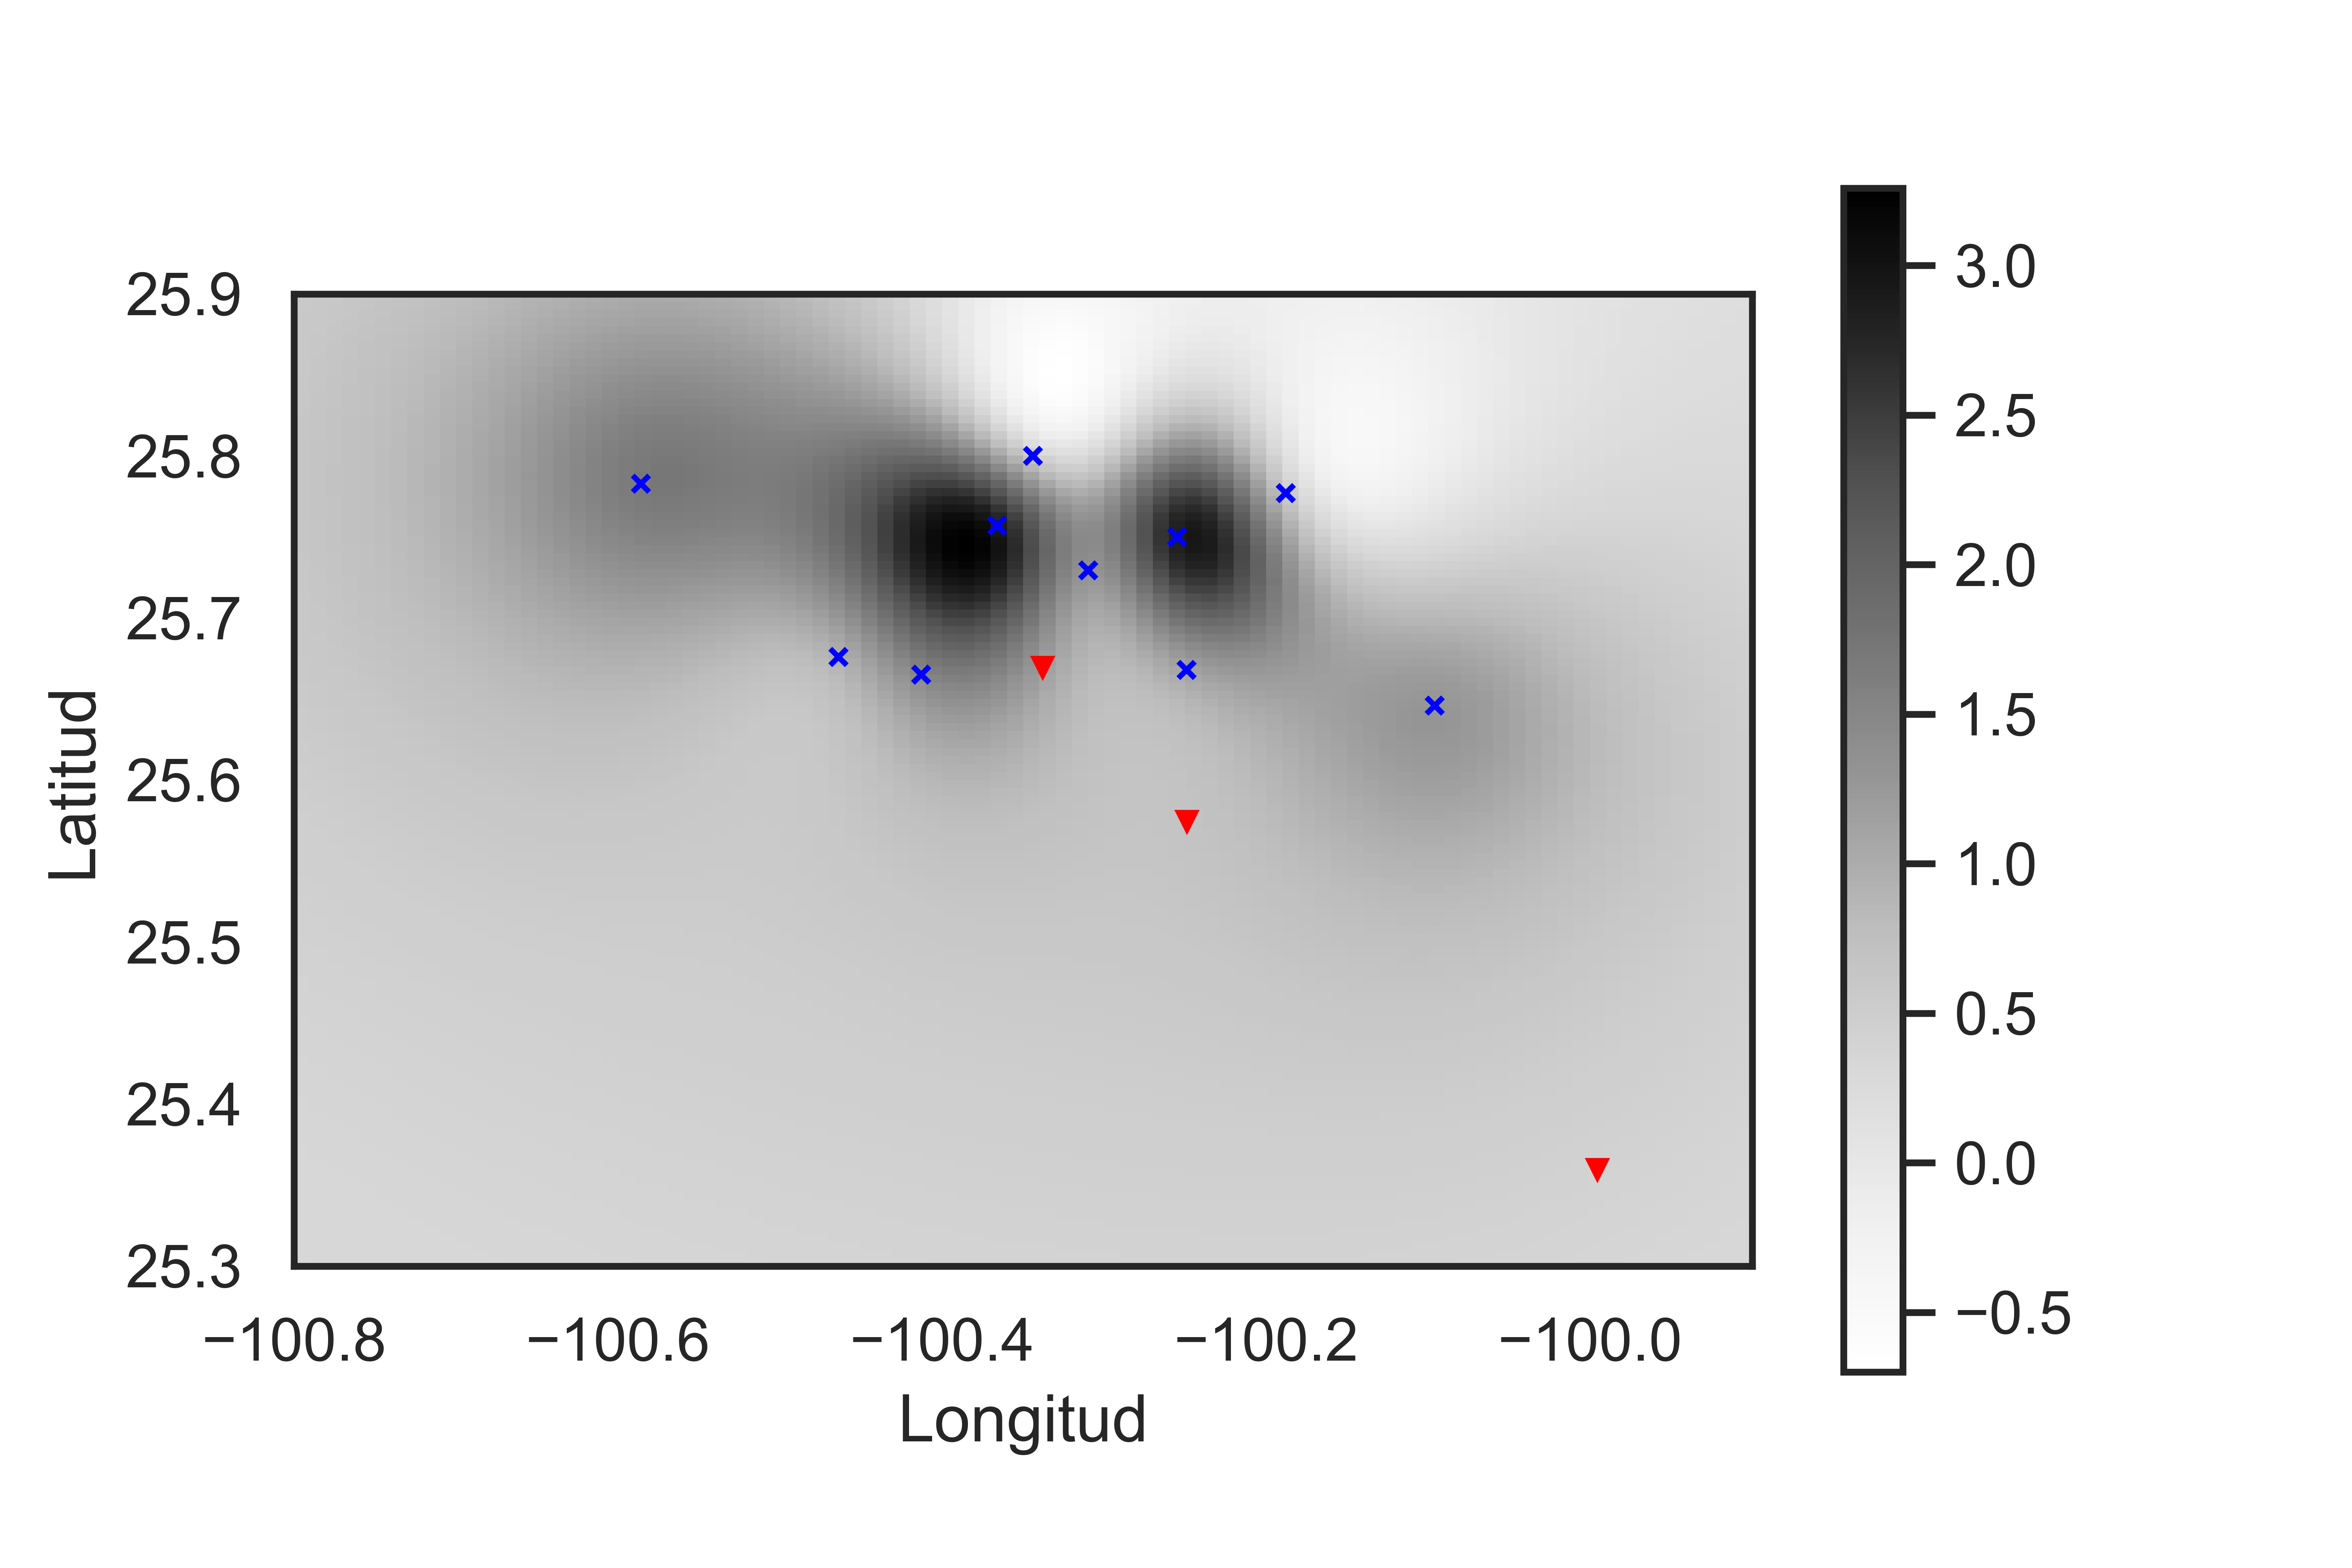
\includegraphics[width=4cm, height=4cm]{./brf_i_10_0_26302}}
\subfigure[FBR G] {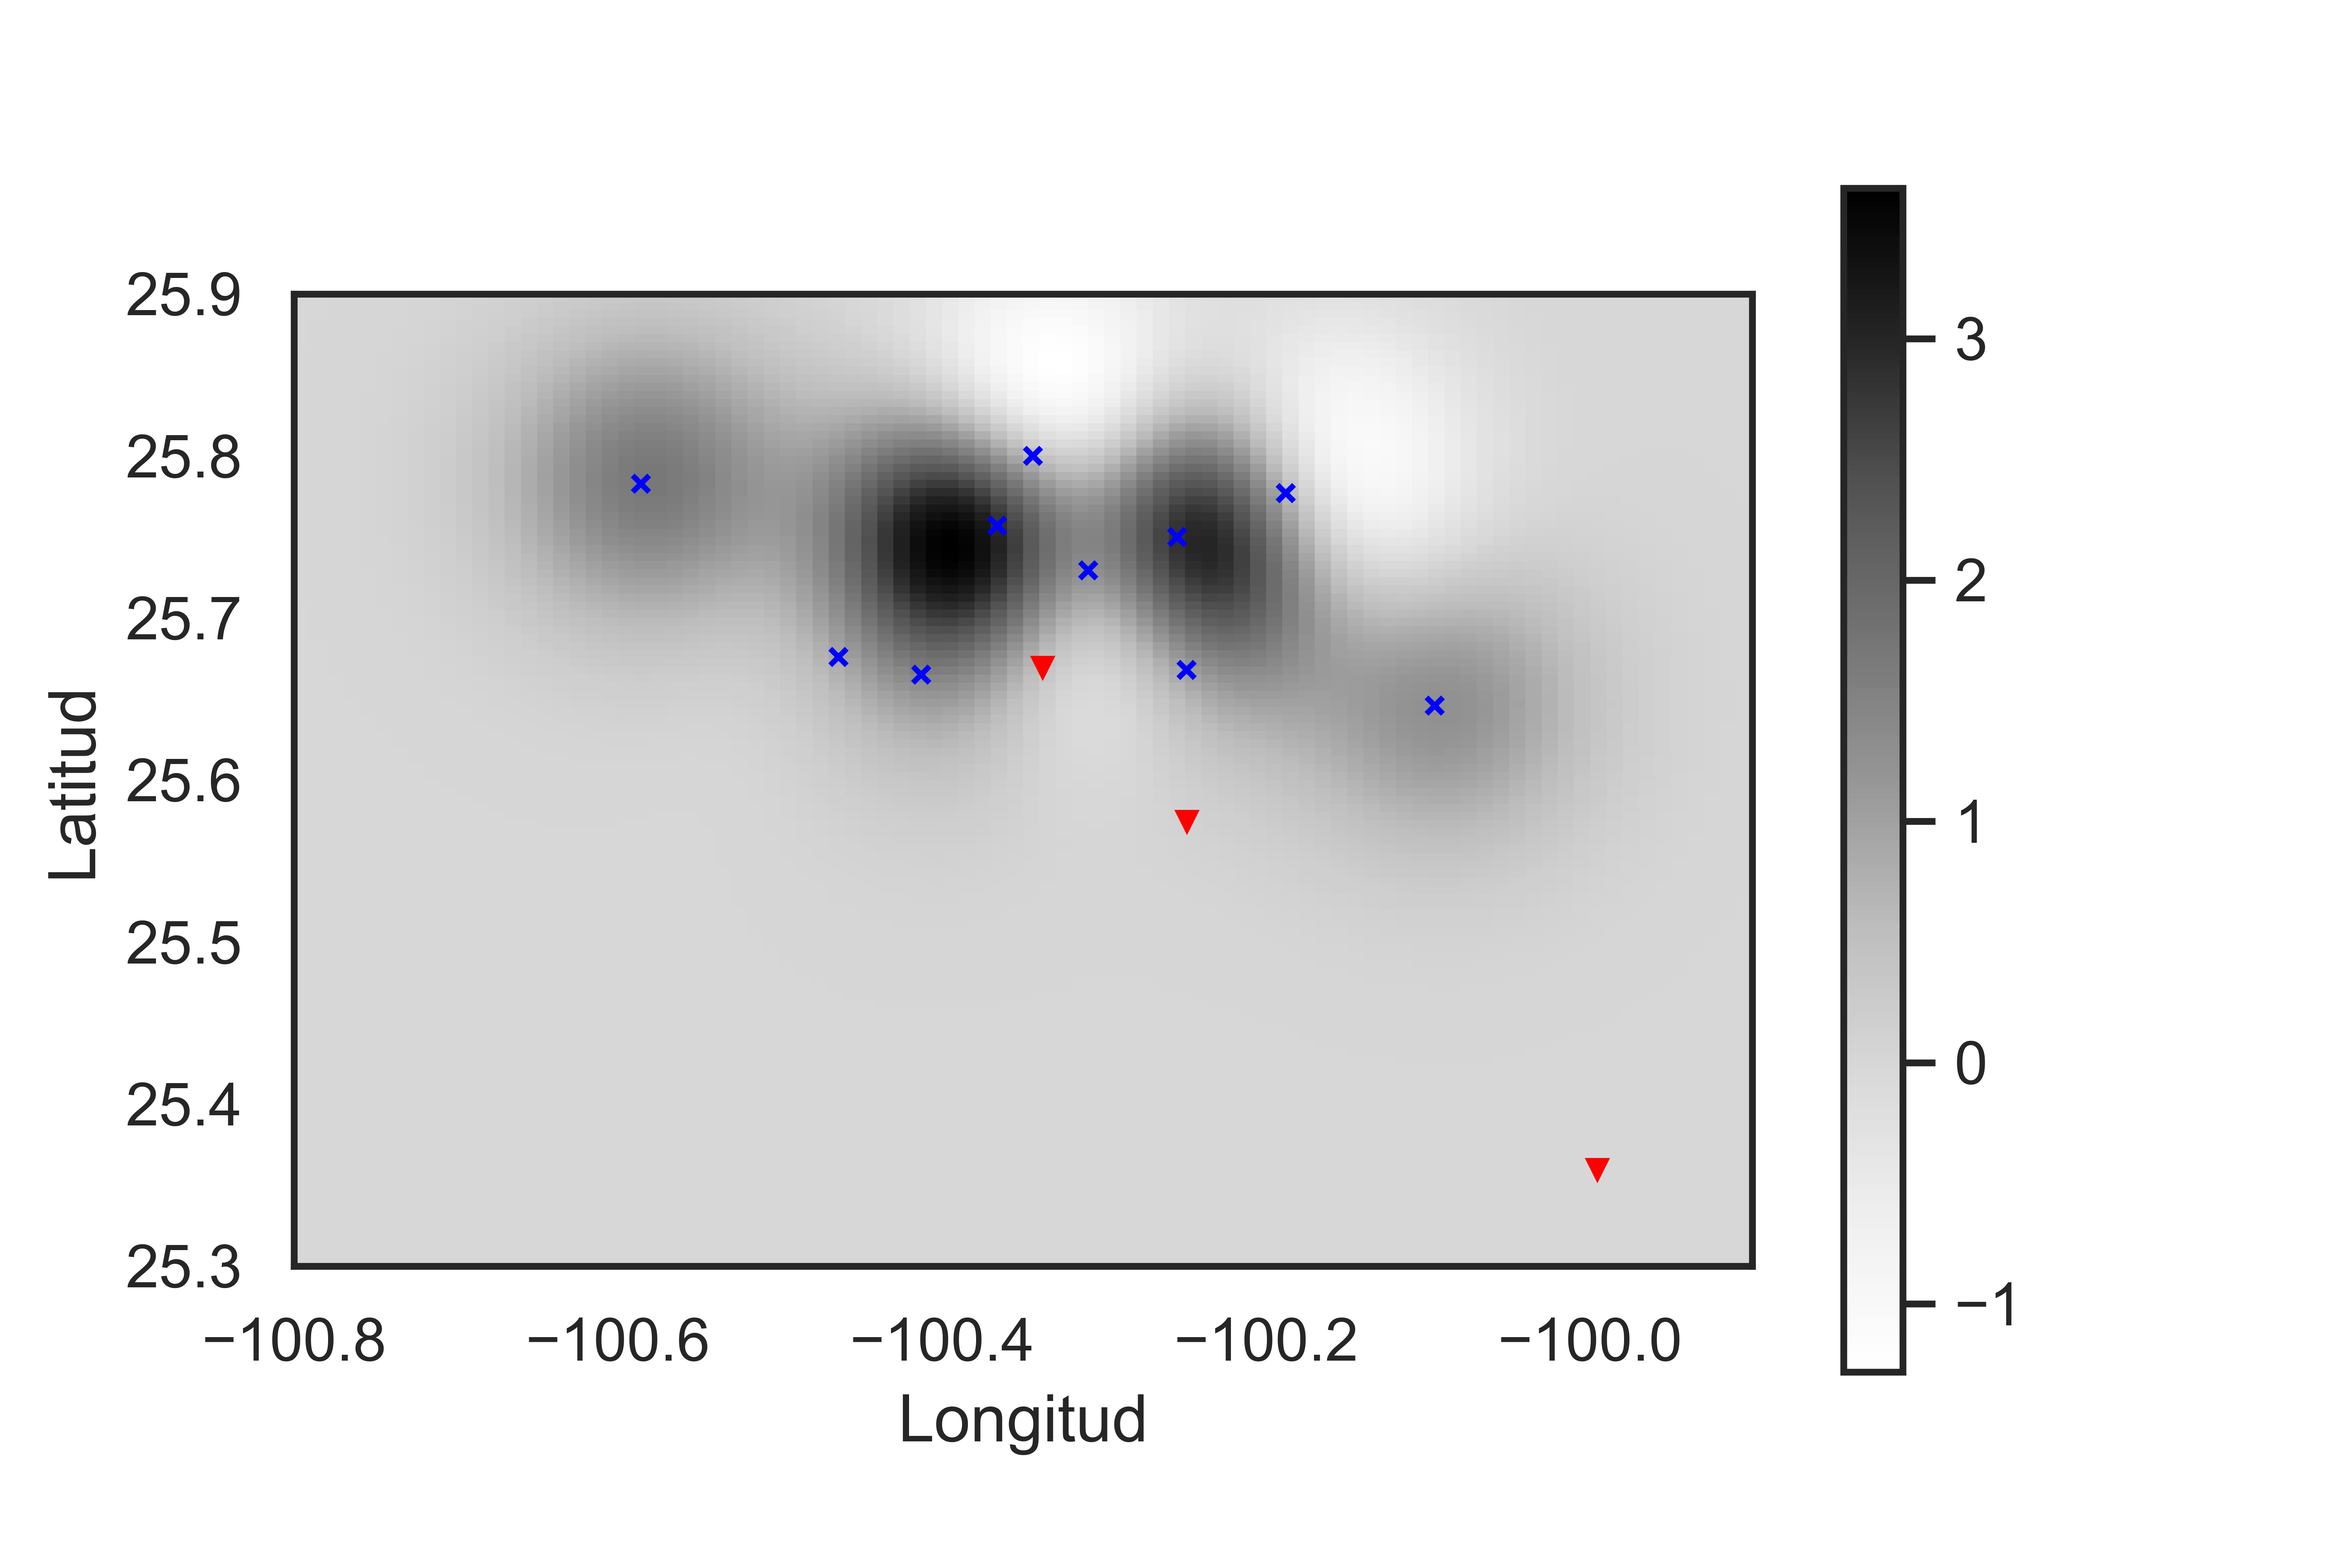
\includegraphics[width=4cm, height=4cm]{./brf_g_10_0_26302}}
\subfigure[FBR L] {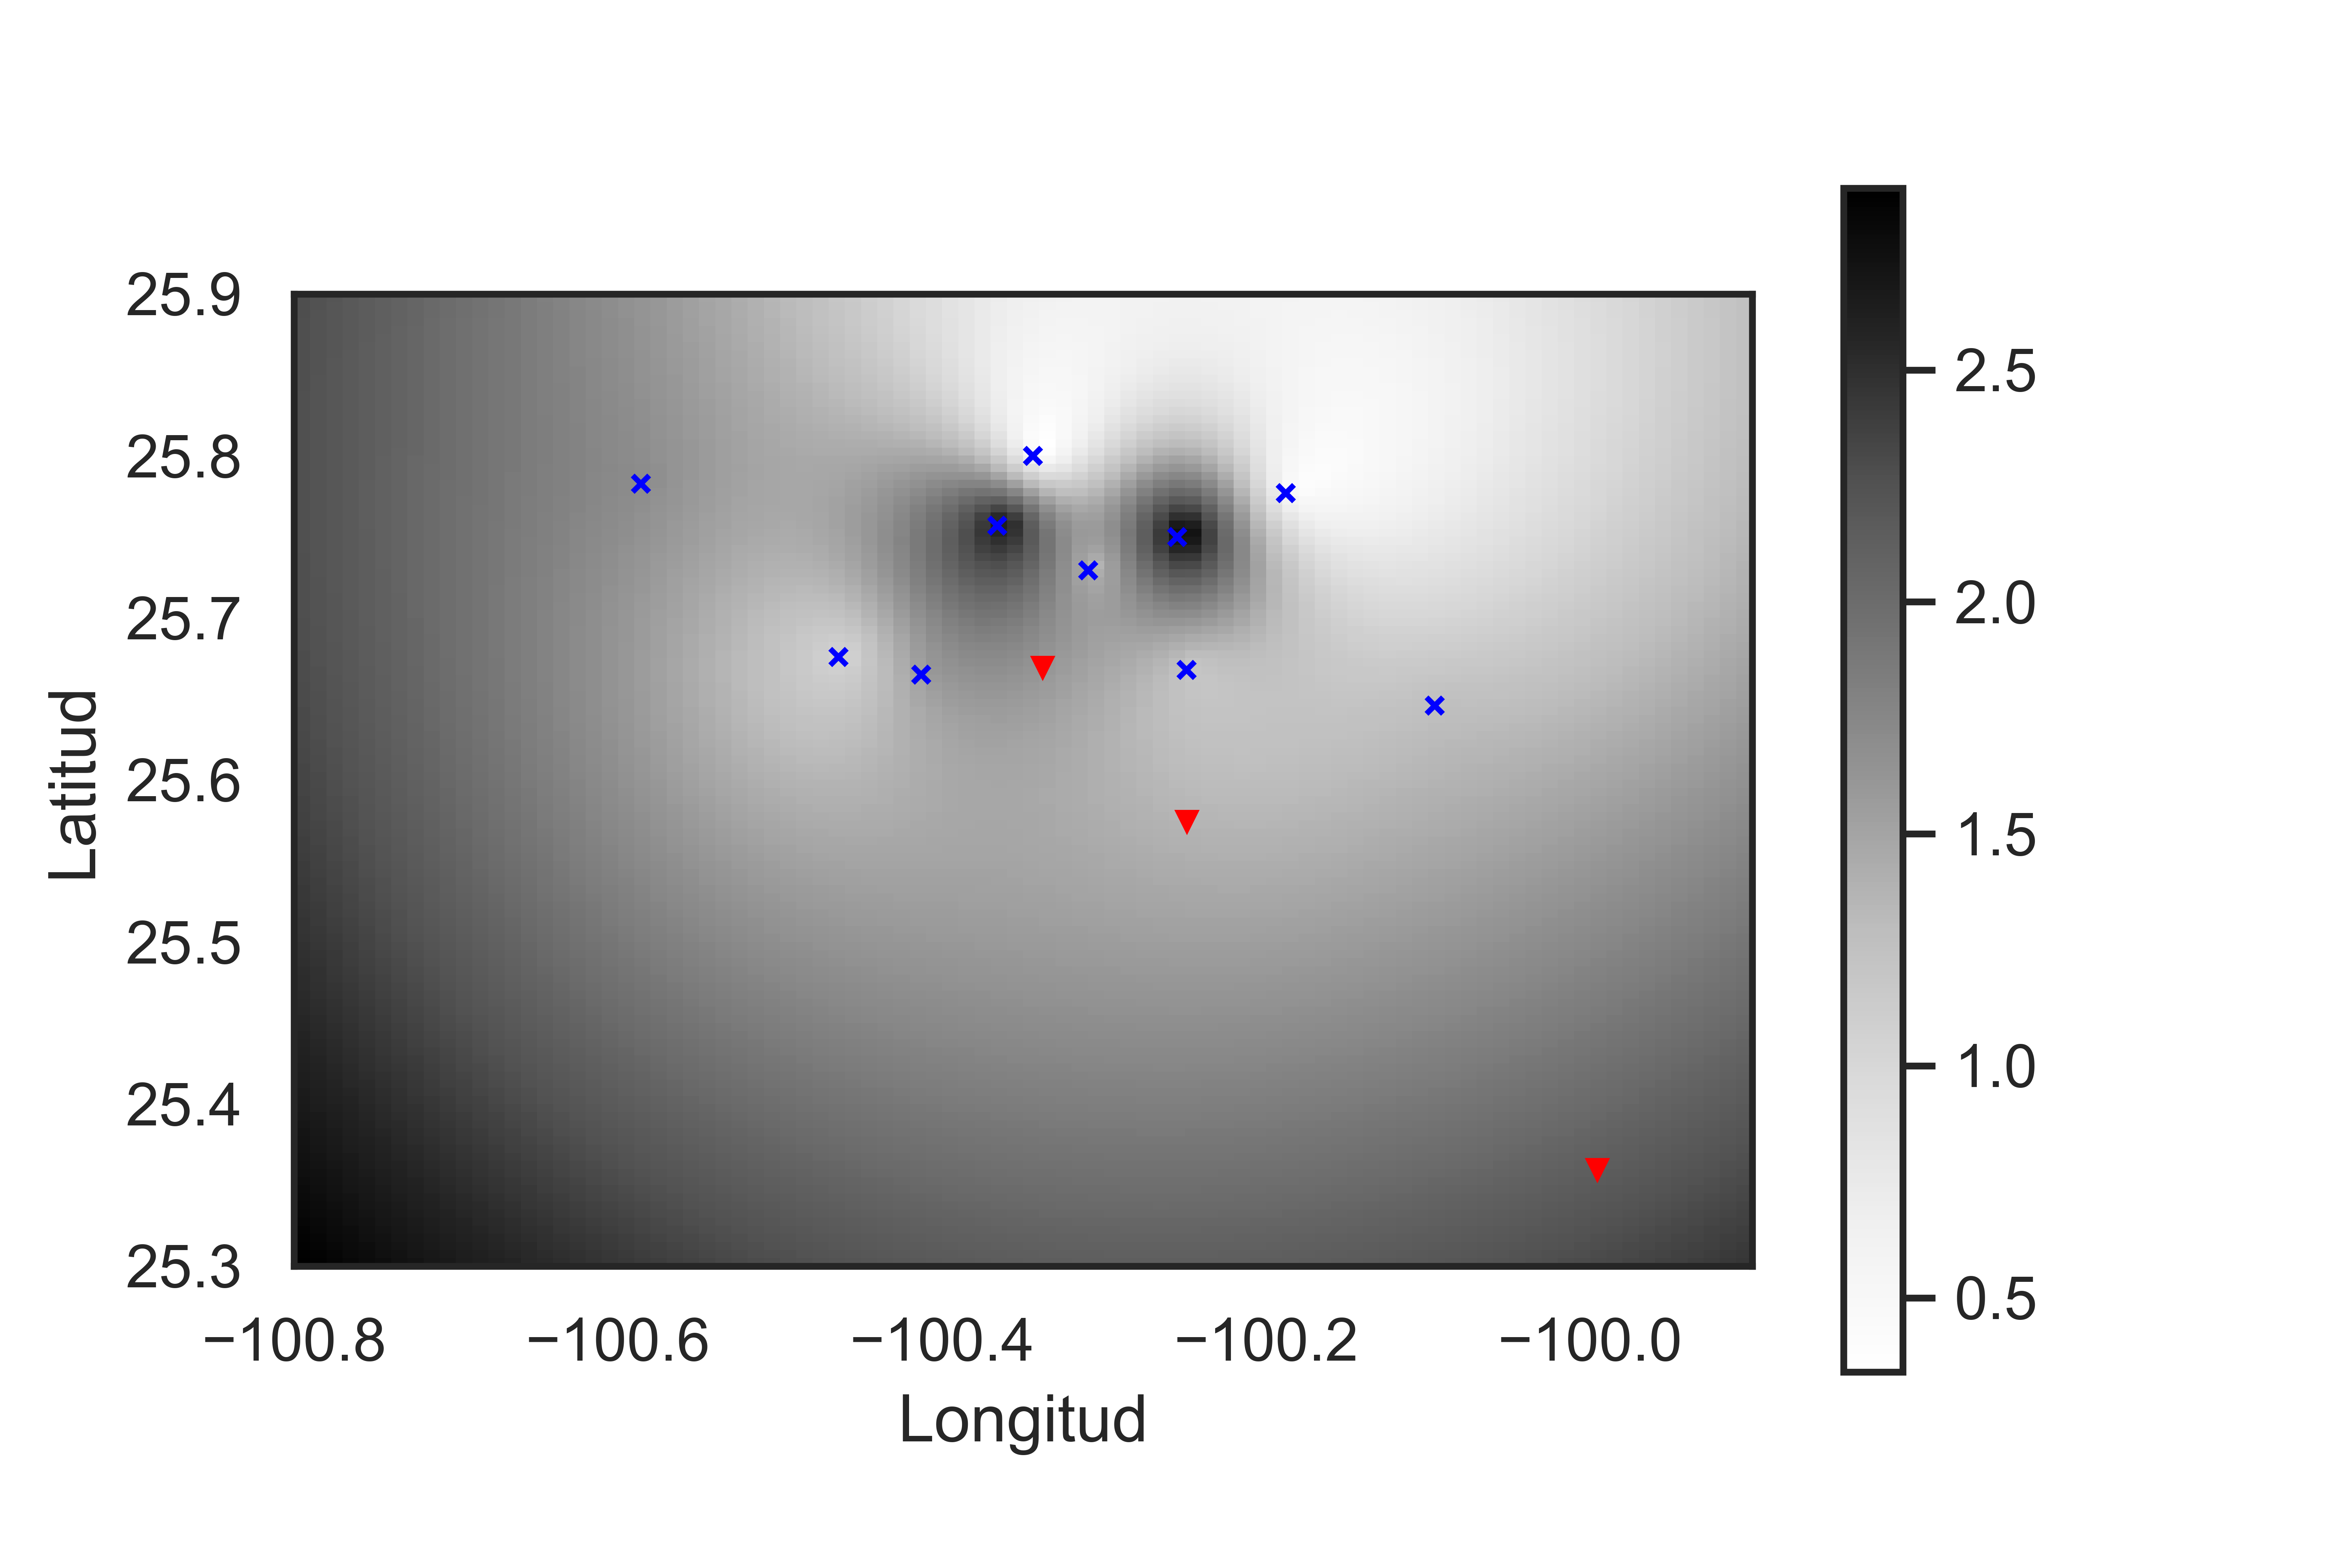
\includegraphics[width=4cm, height=4cm]{./brf_l_10_0_26302}}
\subfigure[FBR C] {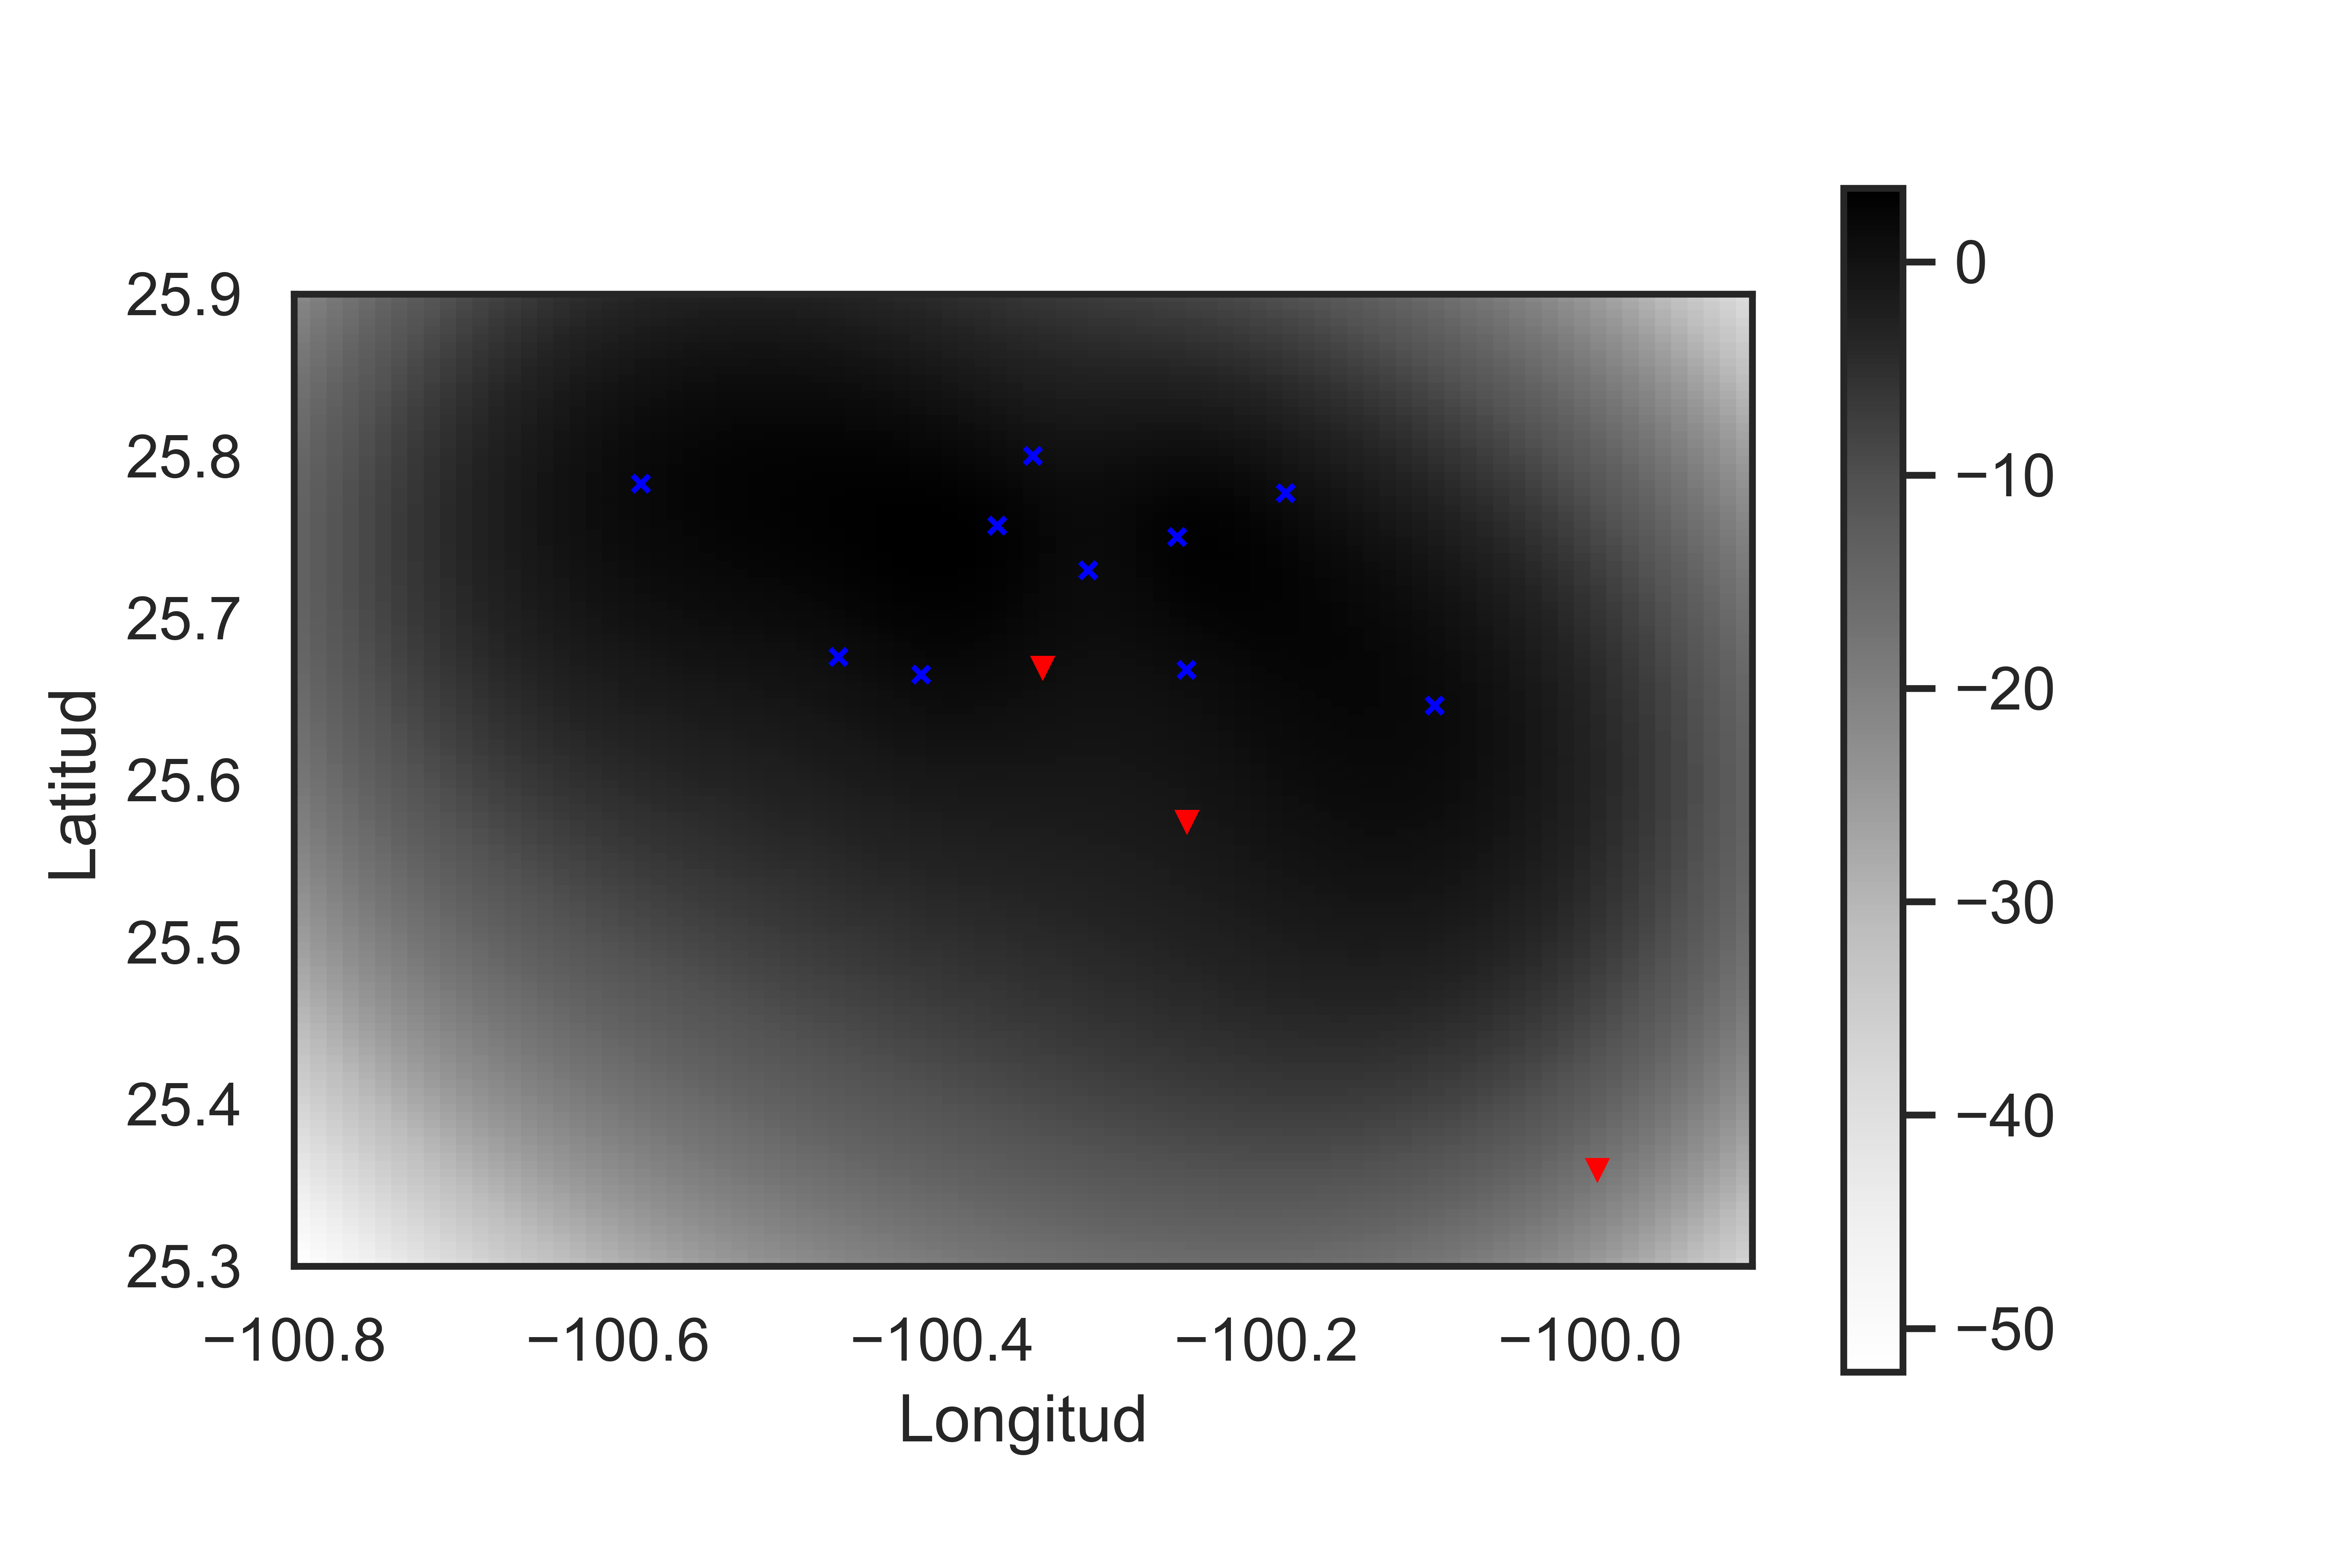
\includegraphics[width=4cm, height=4cm]{./brf_c_10_0_26302}}
\subfigure[FBR Q] {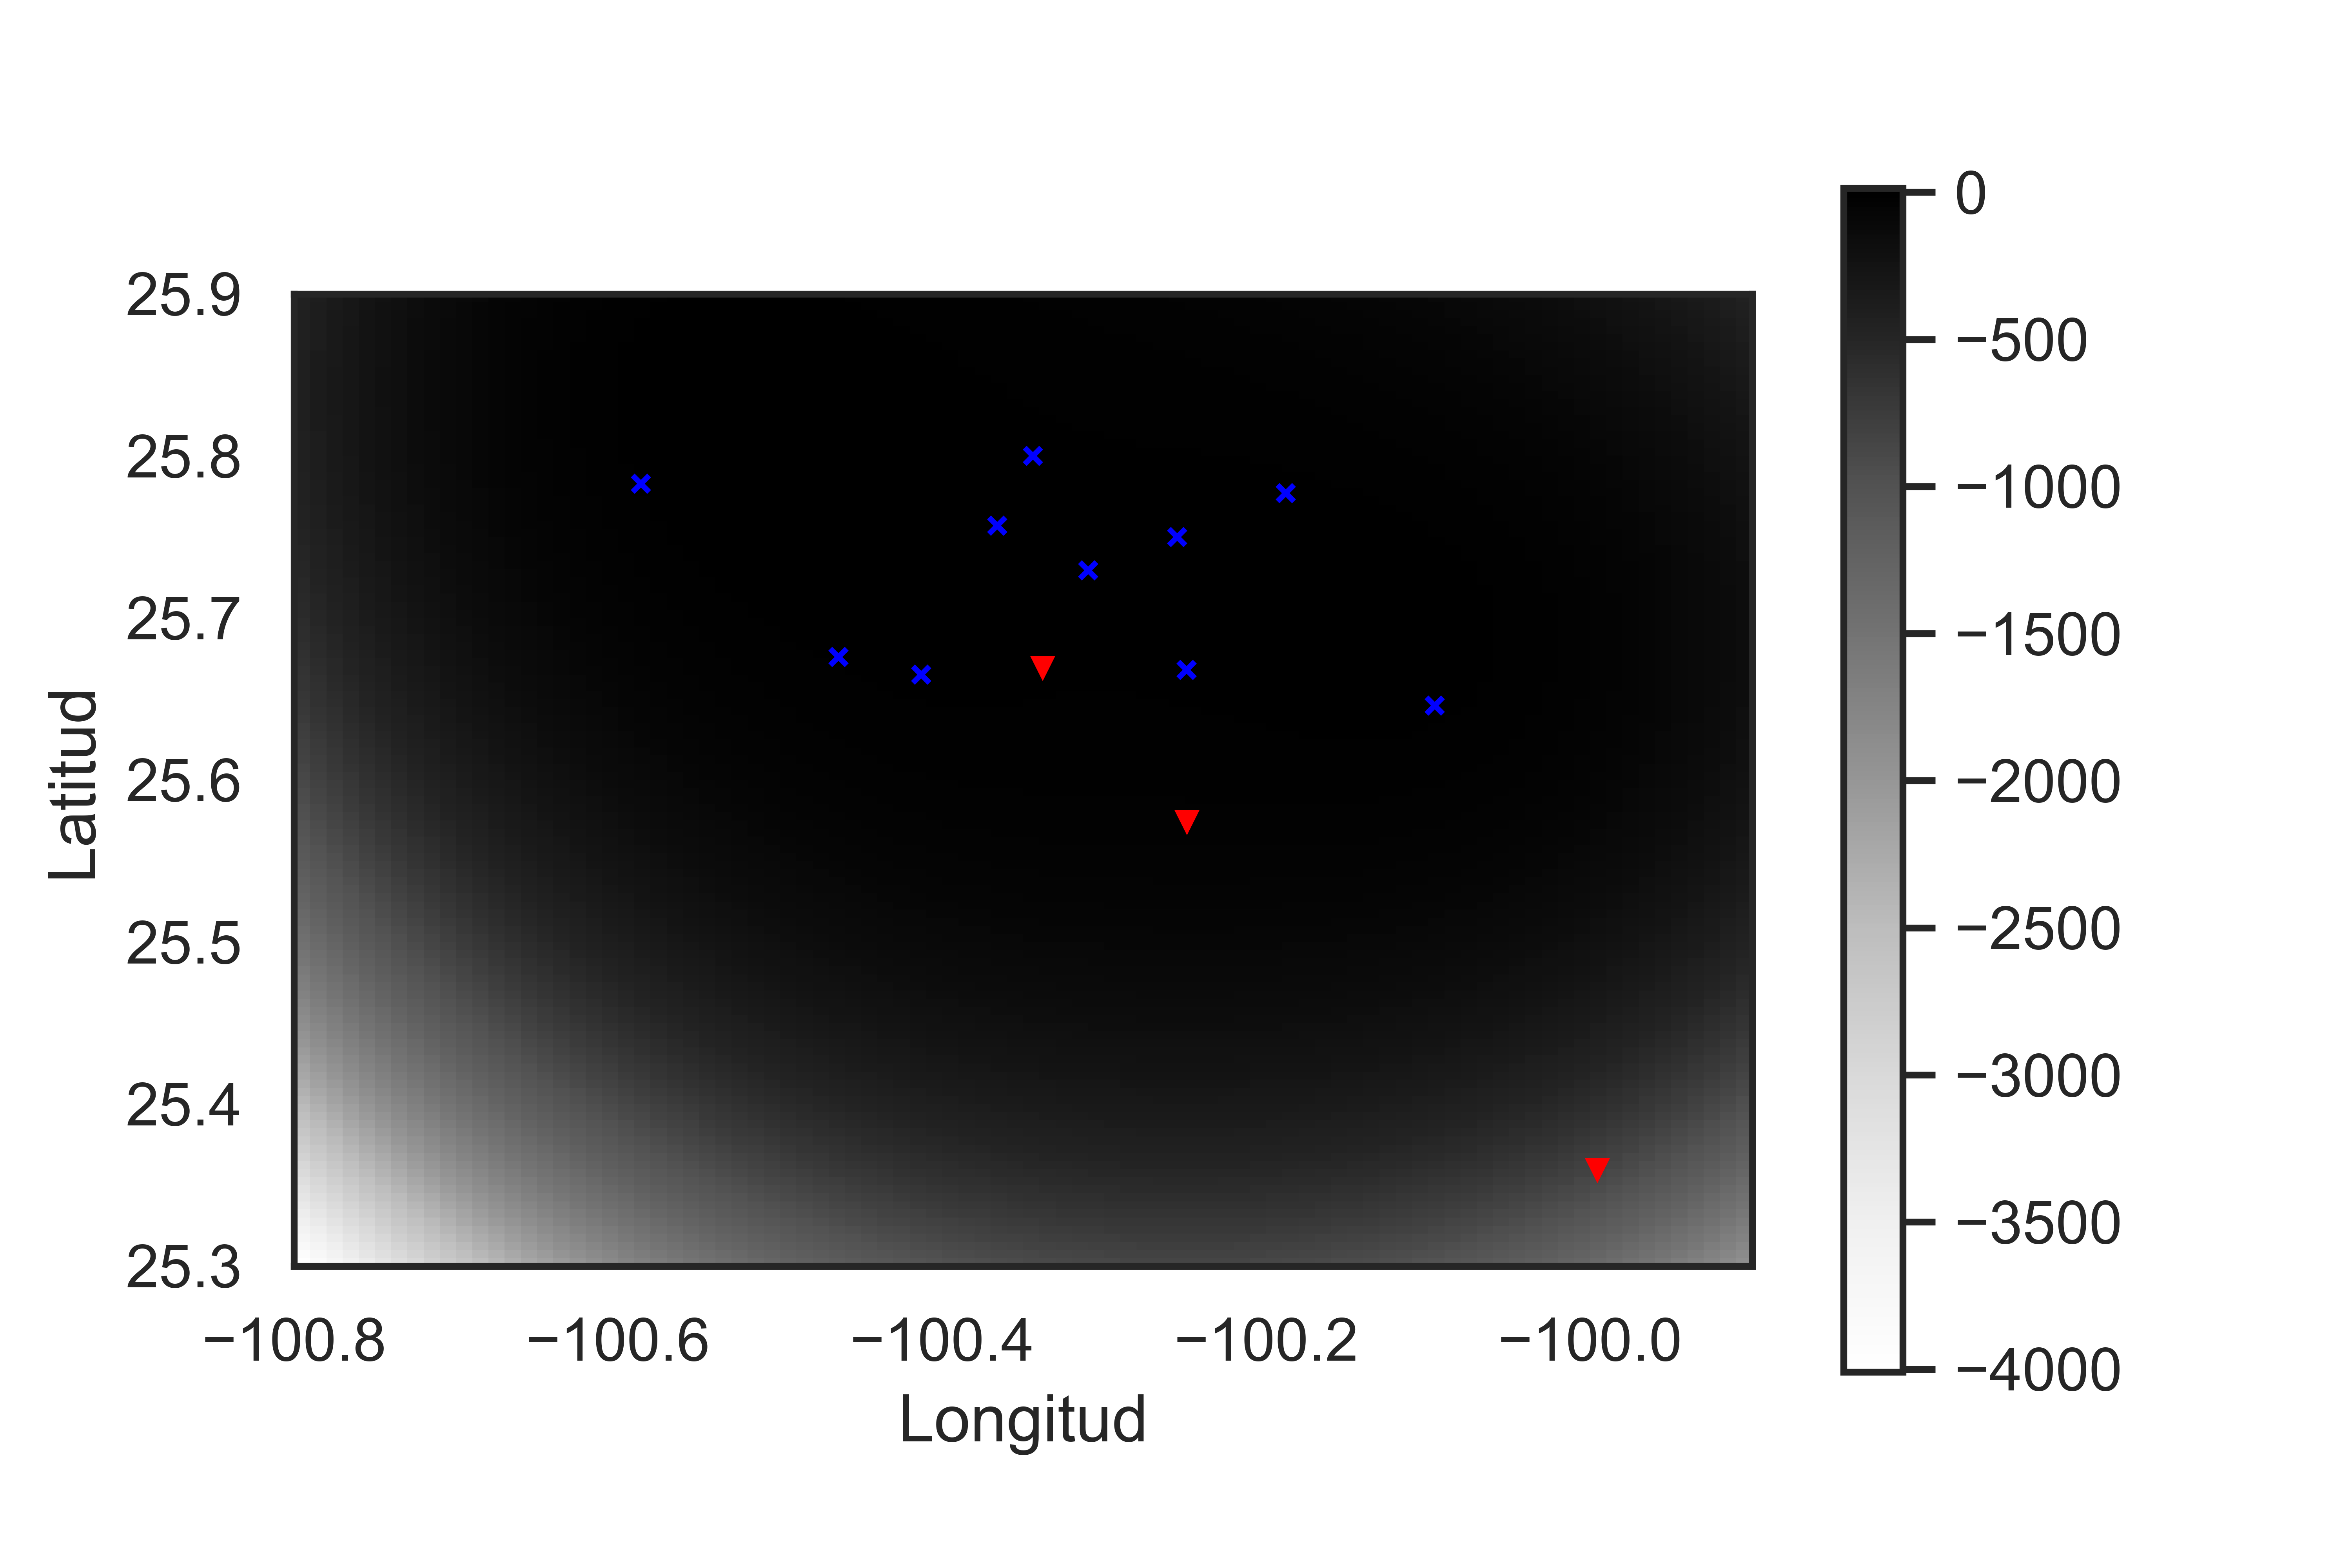
\includegraphics[width=4cm, height=4cm]{./brf_q_10_0_26302}}
\subfigure[FBR TPS] {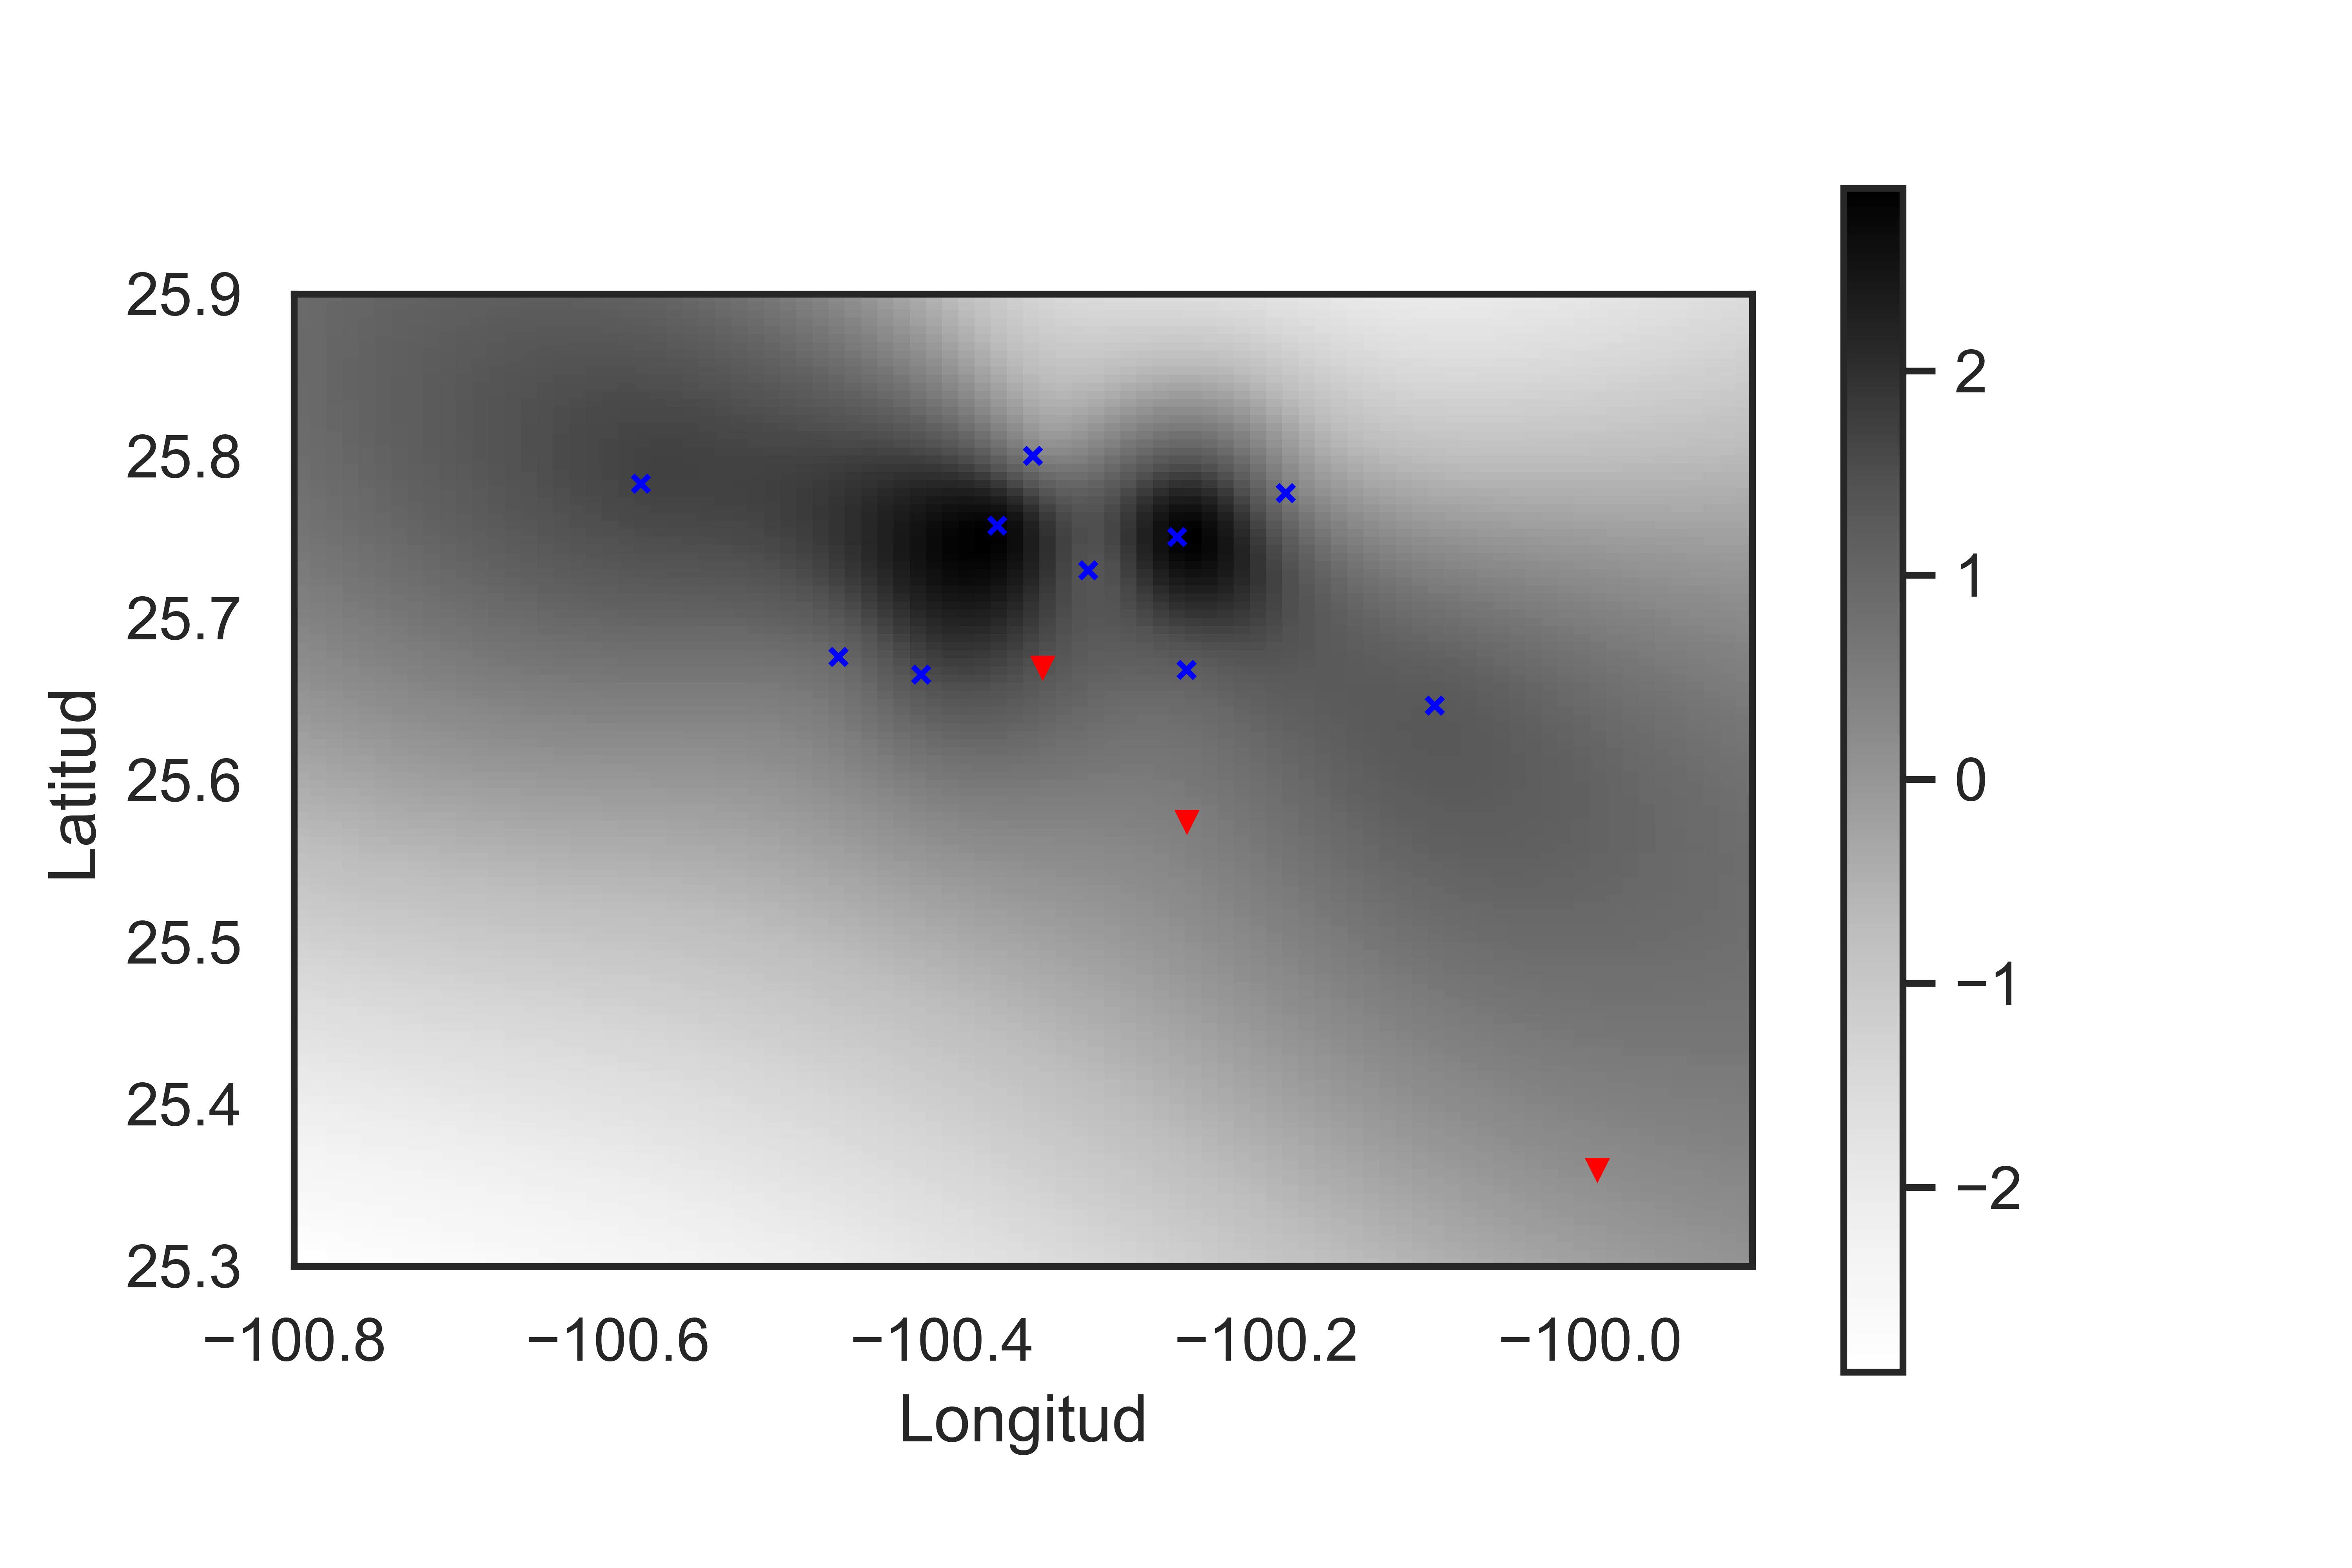
\includegraphics[width=4cm, height=4cm]{./brf_tps_10_0_26302}}
\subfigure[KO] {\includegraphics[width=4cm, height=4cm]{./ok_10_0_26302}}
\subfigure[KU] {\includegraphics[width=4cm, height=4cm]{./uk_10_0_26302}}
\caption{Interpolaciones de CO para 10 estaciones seleccionadas y 3 estaciones interpoladas: Fecha (31-12-2018 23:00:00)}
\label{COfigure2}
\end{figure}


\begin{table}[H]
\centering
\caption{CO: 11 estaciones seleccionadas 2 estaciones interpoladas}
\begin{adjustbox}{max width=0.9\textwidth}
\begin{tabular}{|c|c|c|c|c|c|c|}
\hline
\multicolumn{7}{ |c| }{Métricas de error} \\ \hline
Método &MAPE &MAE &MAEP &RMSE &RMSEP &MSE \\ \hline
TV &1.07 &0.94 &0.70 &1.25 &0.93 &1.56 \\
DIP &0.89 &0.89 &0.67 &1.12 &0.84 &1.25 \\
FBR M &$1.79\times10^{17}$ &$2.51\times10^{17}$ &$1.88\times10^{17}$ &$1.52\times10^{18}$ &$1.14\times10^{18}$ &$2.31\times10^{36}$ \\
FBR IM &1.23 &1.16 &0.87 &1.65 &1.24 &2.72 \\
FBR G &$6.06\times10^{16}$ &$5.25\times10^{15}$ &$3.95\times10^{15}$ &$2.20\times10^{17}$ &$1.65\times10^{17}$ &$4.85\times10^{34}$ \\
FBR L &1.10 &1.01 &0.76 &1.32 &0.99 &1.75 \\
FBR C &$5.92\times10^{17}$ &$5.94\times10^{17}$ &$4.46\times10^{17}$ &$2.34\times10^{18}$ &$1.75\times10^{18}$ &$5.48\times10^{36}$ \\
FBR Q &$2.04\times10^{18}$ &$1.52\times10^{18}$ &$1.14\times10^{18}$ &$3.75\times10^{18}$ &$2.82\times10^{18}$ &$1.41\times10^{37}$ \\
FBR TPS &$3.71\times10^{14}$ &$3.50\times10^{15}$ &$2.63\times10^{14}$ &$5.68\times10^{16}$ &$4.27\times10^{16}$ &$3.23\times10^{33}$ \\
KO &0.87 &0.88 &0.66 &1.11 &0.83 &1.23 \\
KU &1.11 &0.98 &0.74 &1.34 &1.01 &1.82 \\\hline
\end{tabular}
\end{adjustbox}
\label{tabCO_3}
\end{table}


De la tabla \ref{tabCO_3}, en la cual se utilizan once estaciones para interpolar dos más, podemos ver que los métodos que obtiene peores resultados de predicción son los métodos de Funciones de Base Radial, a excepción de los métodos inverso multicuadrático y lineal (FBR I y FBR L). Entre los métodos deterministas, DIP obtuvo el menor MAPE, MAE, MAEP, RMSE, RMSEP y MSE, mientras que de los métodos geoestadísticos el método KO obtuvo el menor MAPE, MAE, MAEP, RMSE, RMSEP y MSE; en general DIP y KO son mejores que el resto de los métodos pero KO es mejor que DIP ya que obtuvo en los errores MAPE, MAE, MAEP, RMSE, RMSEP y MSE mejores resultados que los de DIP. En la figura \ref{COfigure3}, se pueden observar las interpolaciones de cada método, donde las puntos azules son las estaciones seleccionadas y los puntos rojos son las estaciones interpoladas.


\begin{figure}[H]
\centering
\subfigure[TV] {\includegraphics[width=4cm, height=4cm]{./voronoi_11_0_26302}}
\subfigure[DIP] {\includegraphics[width=4cm, height=4cm]{./idw_11_0_26302}}
\subfigure[FBR M] {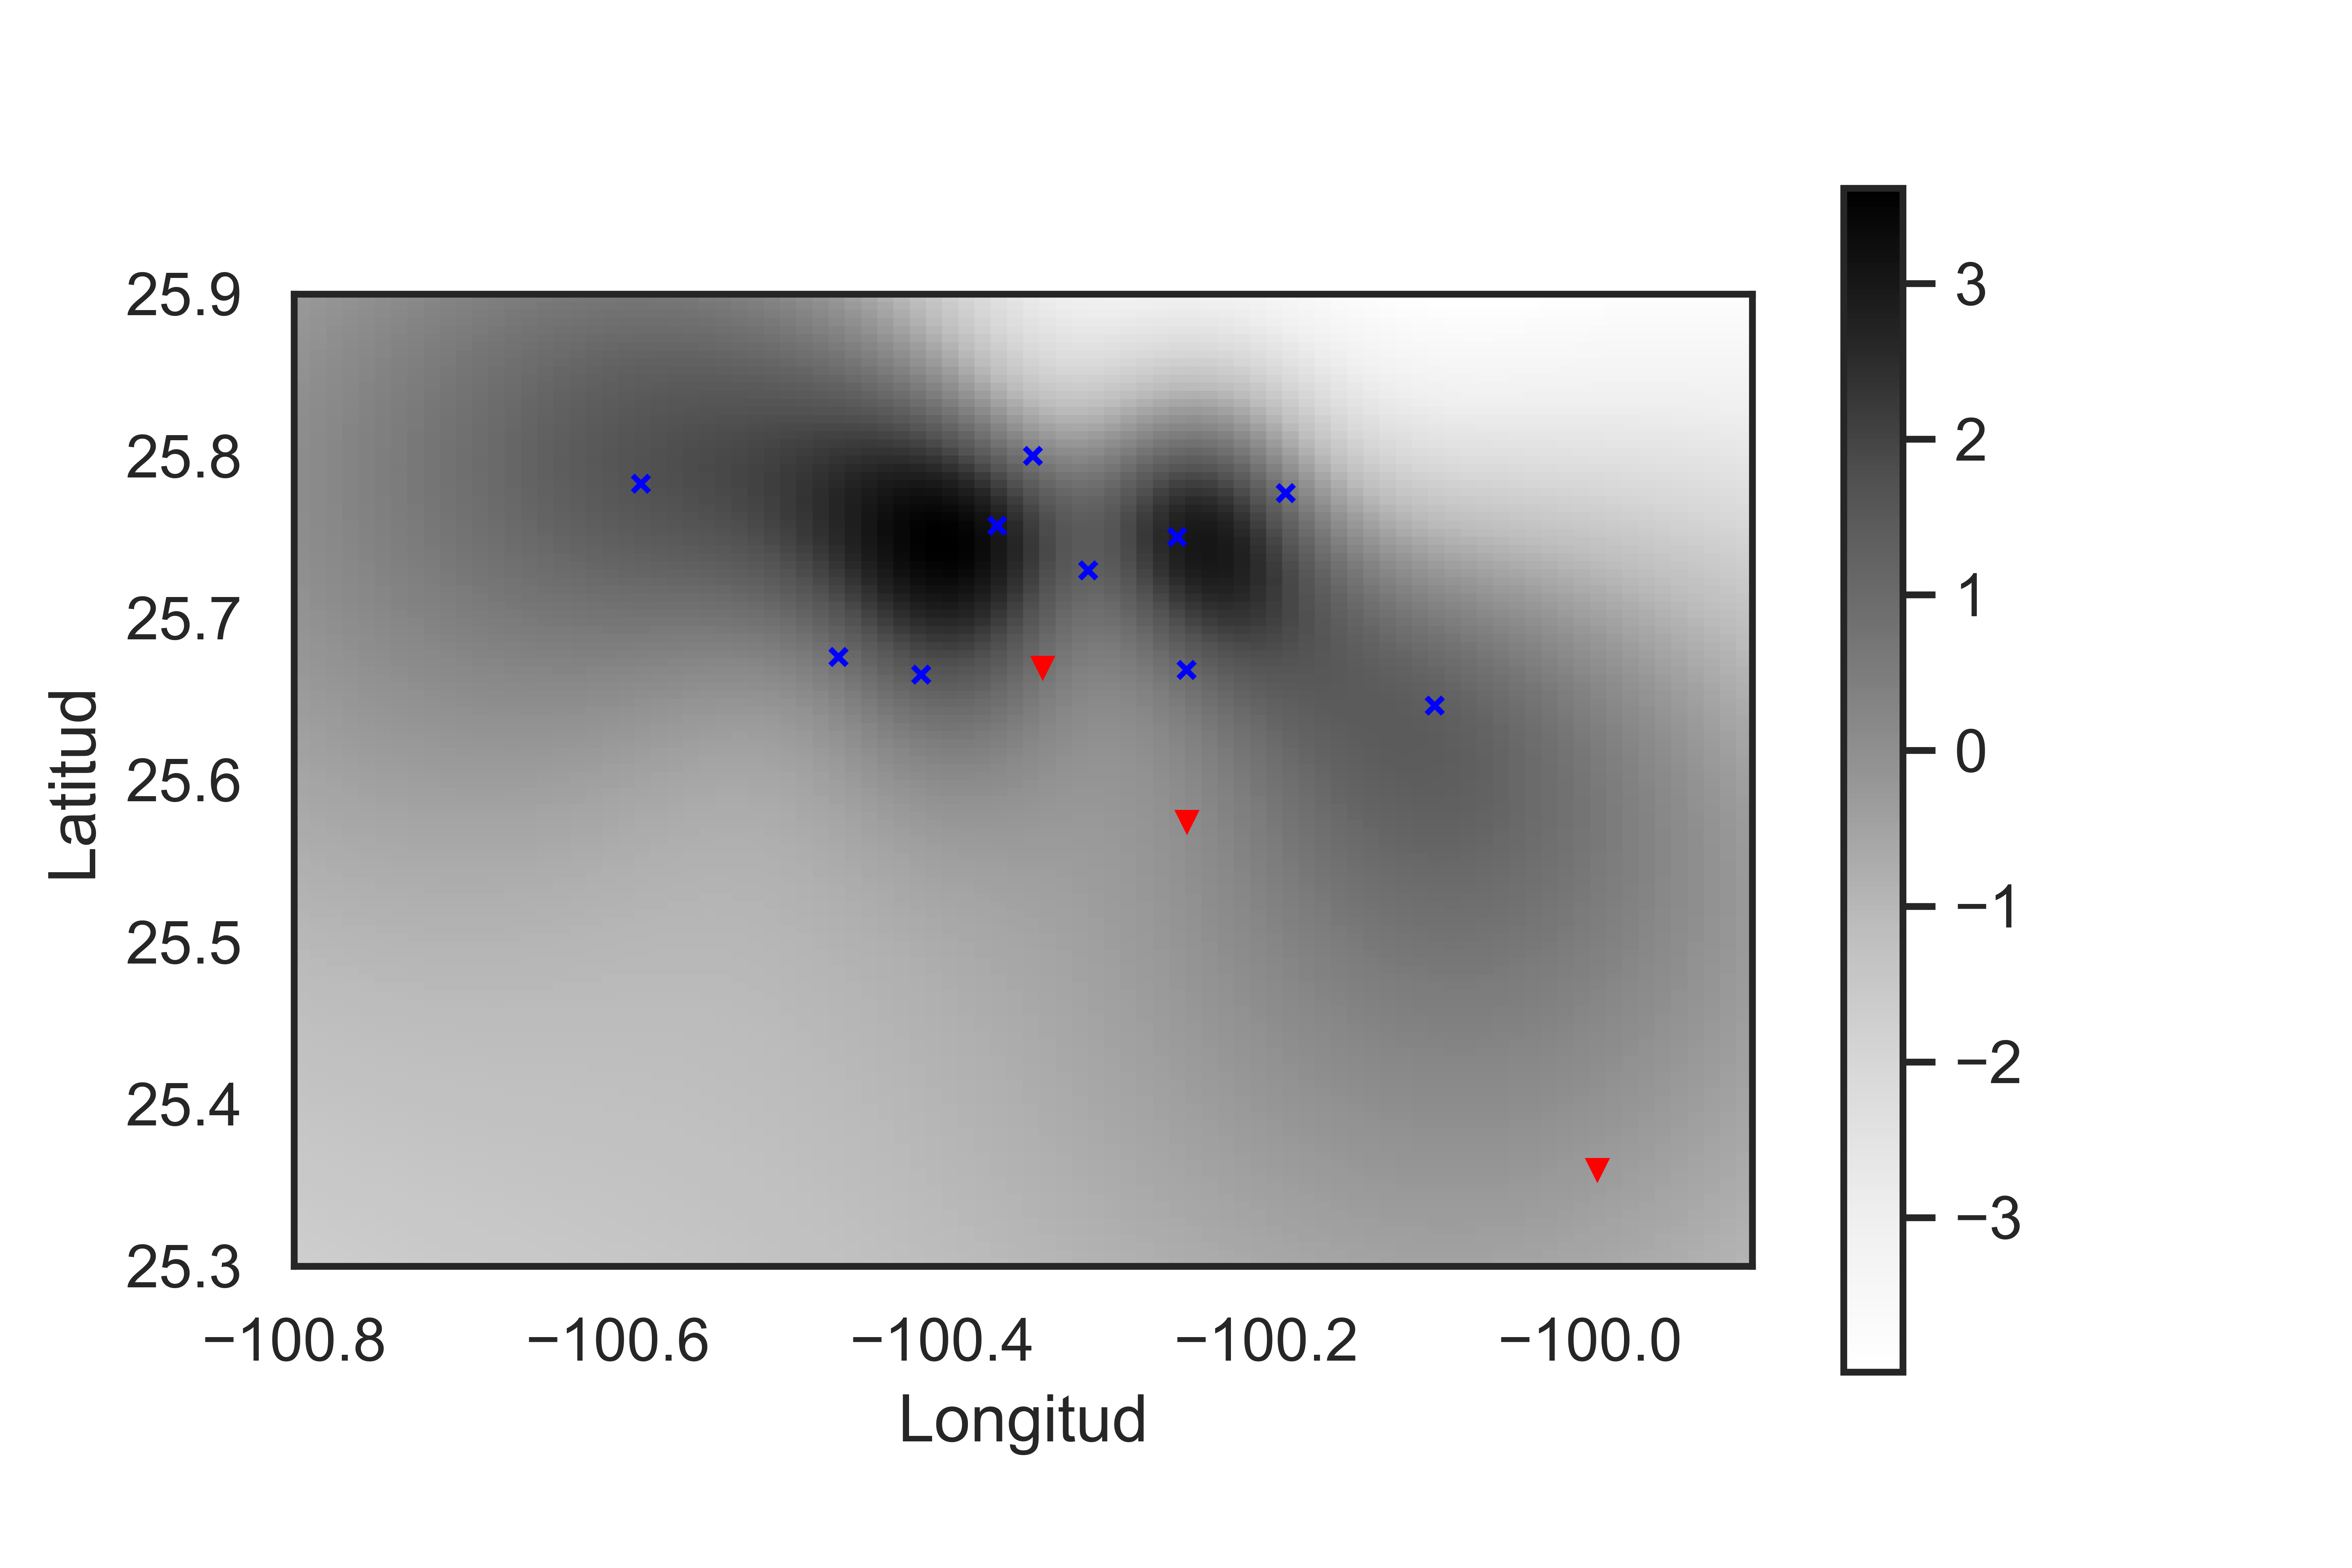
\includegraphics[width=4cm, height=4cm]{./brf_m_11_0_26302}}
\subfigure[FBR I] {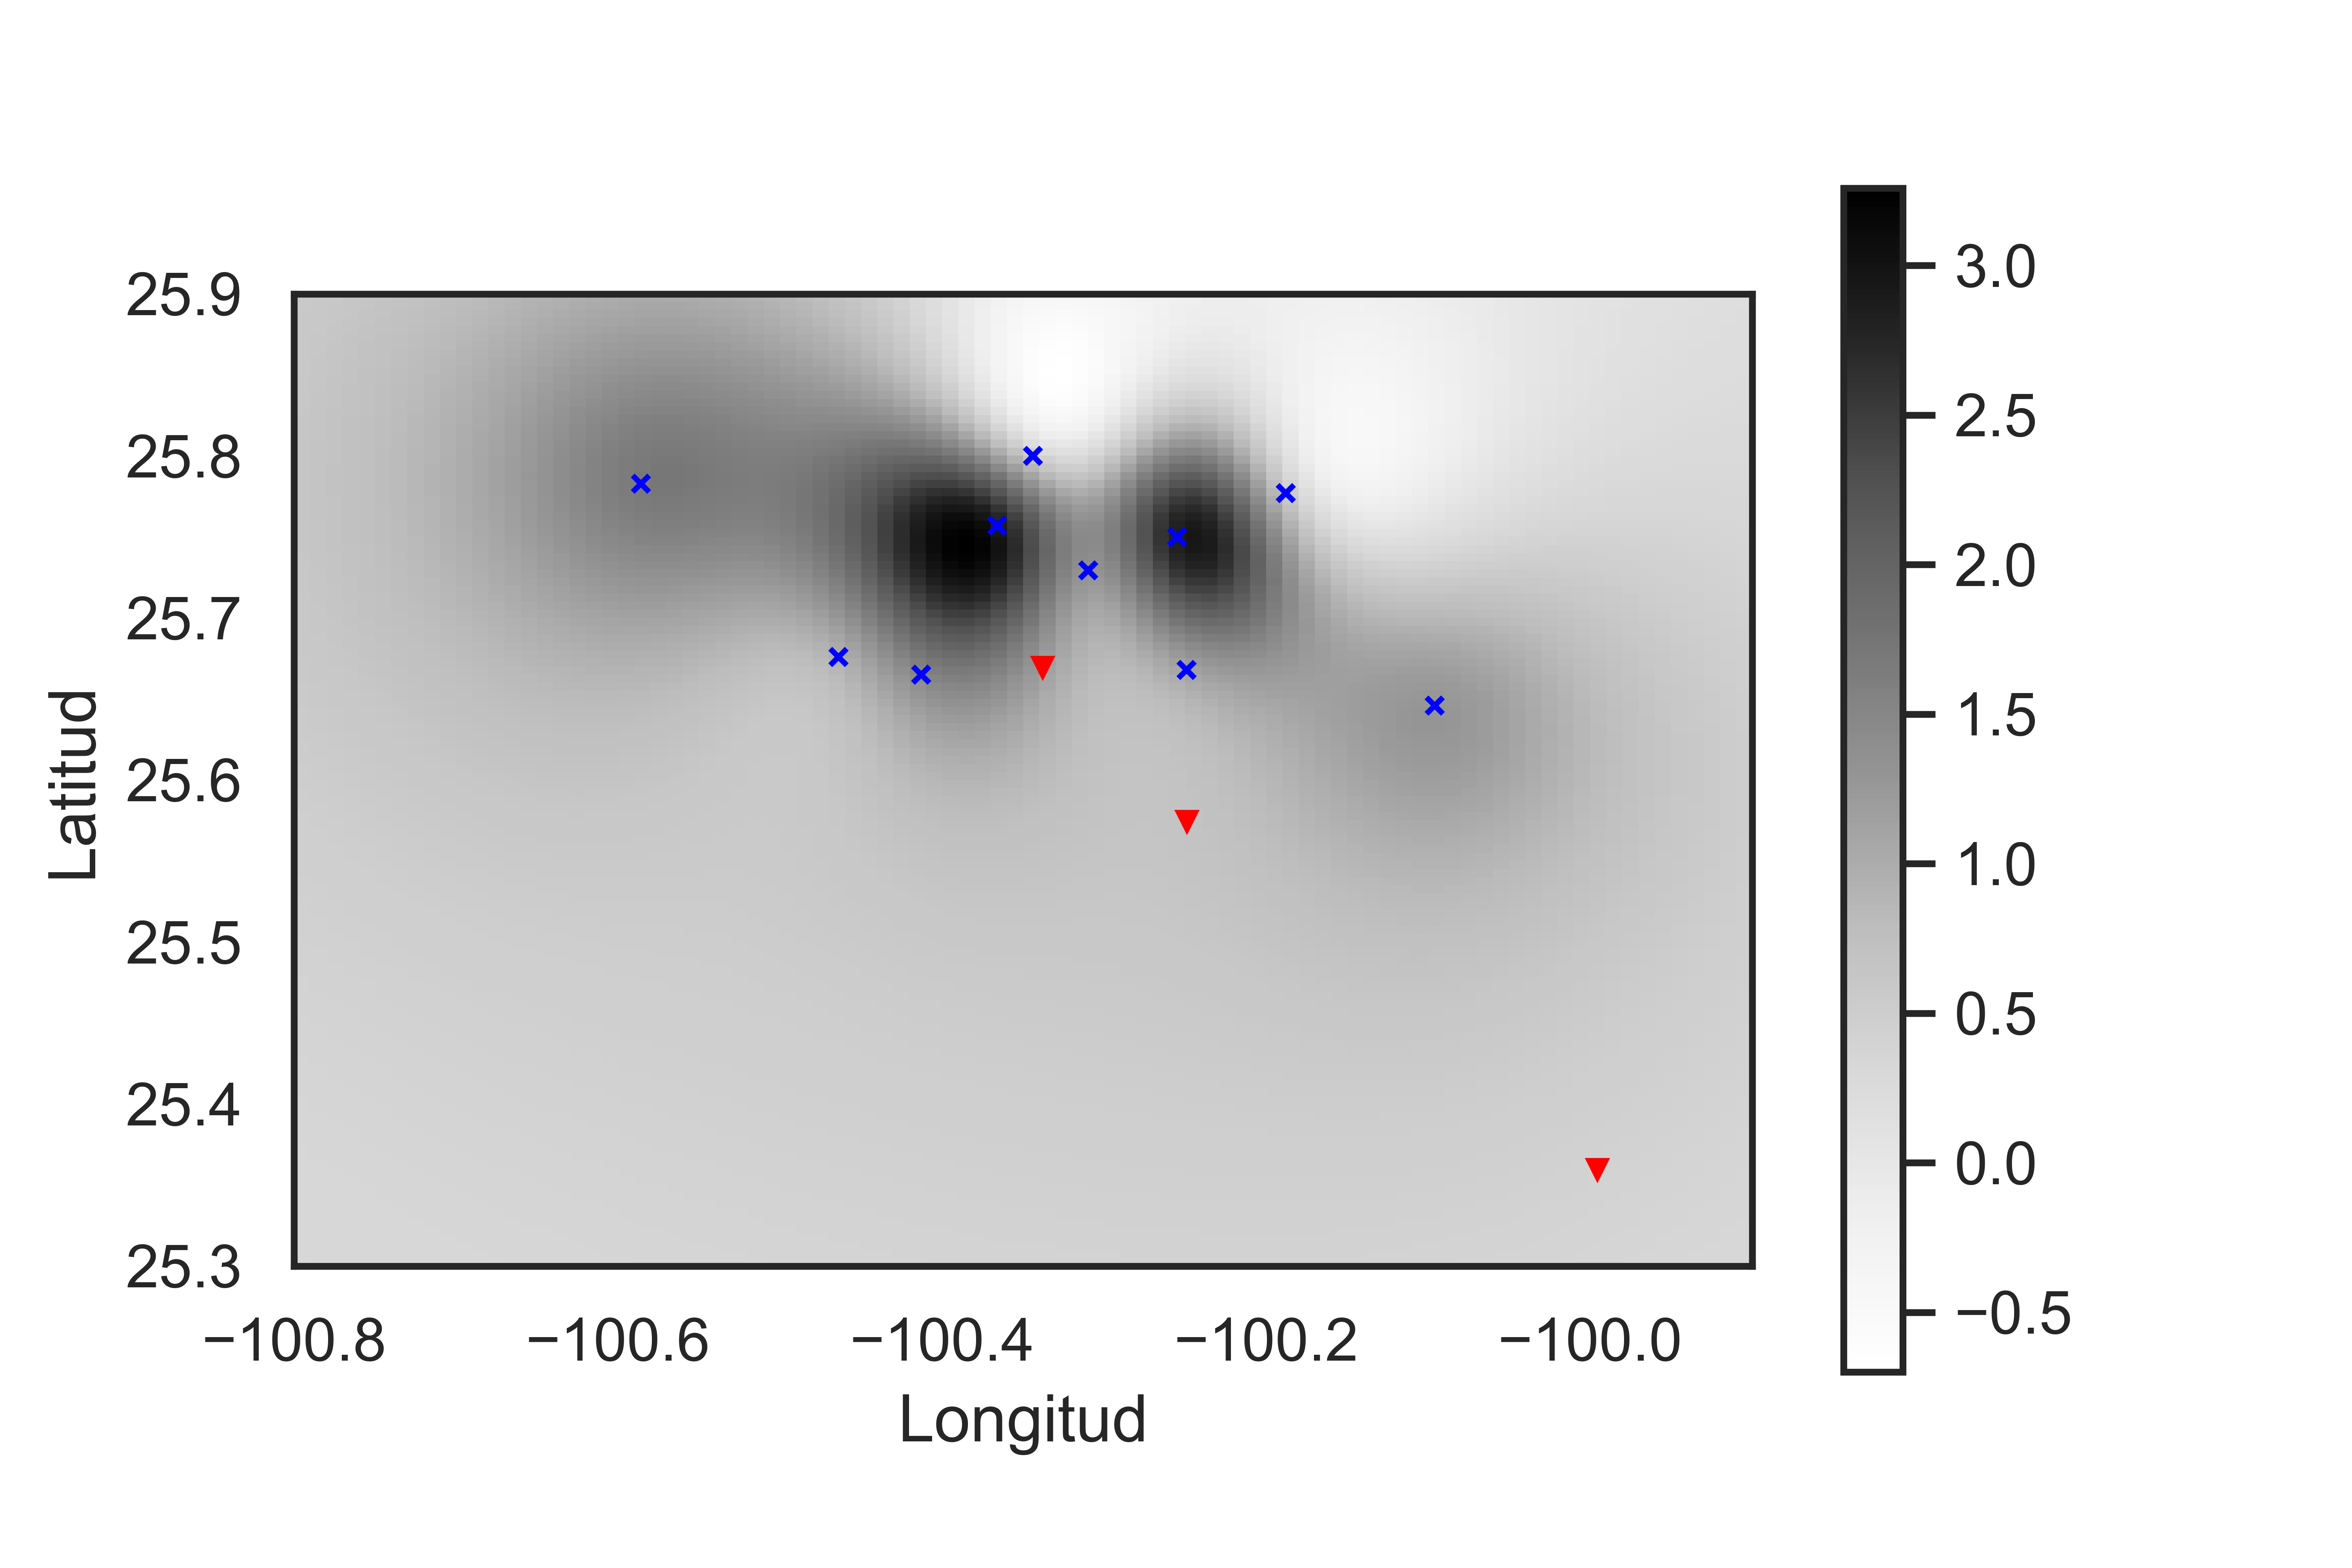
\includegraphics[width=4cm, height=4cm]{./brf_i_11_0_26302}}
\subfigure[FBR G] {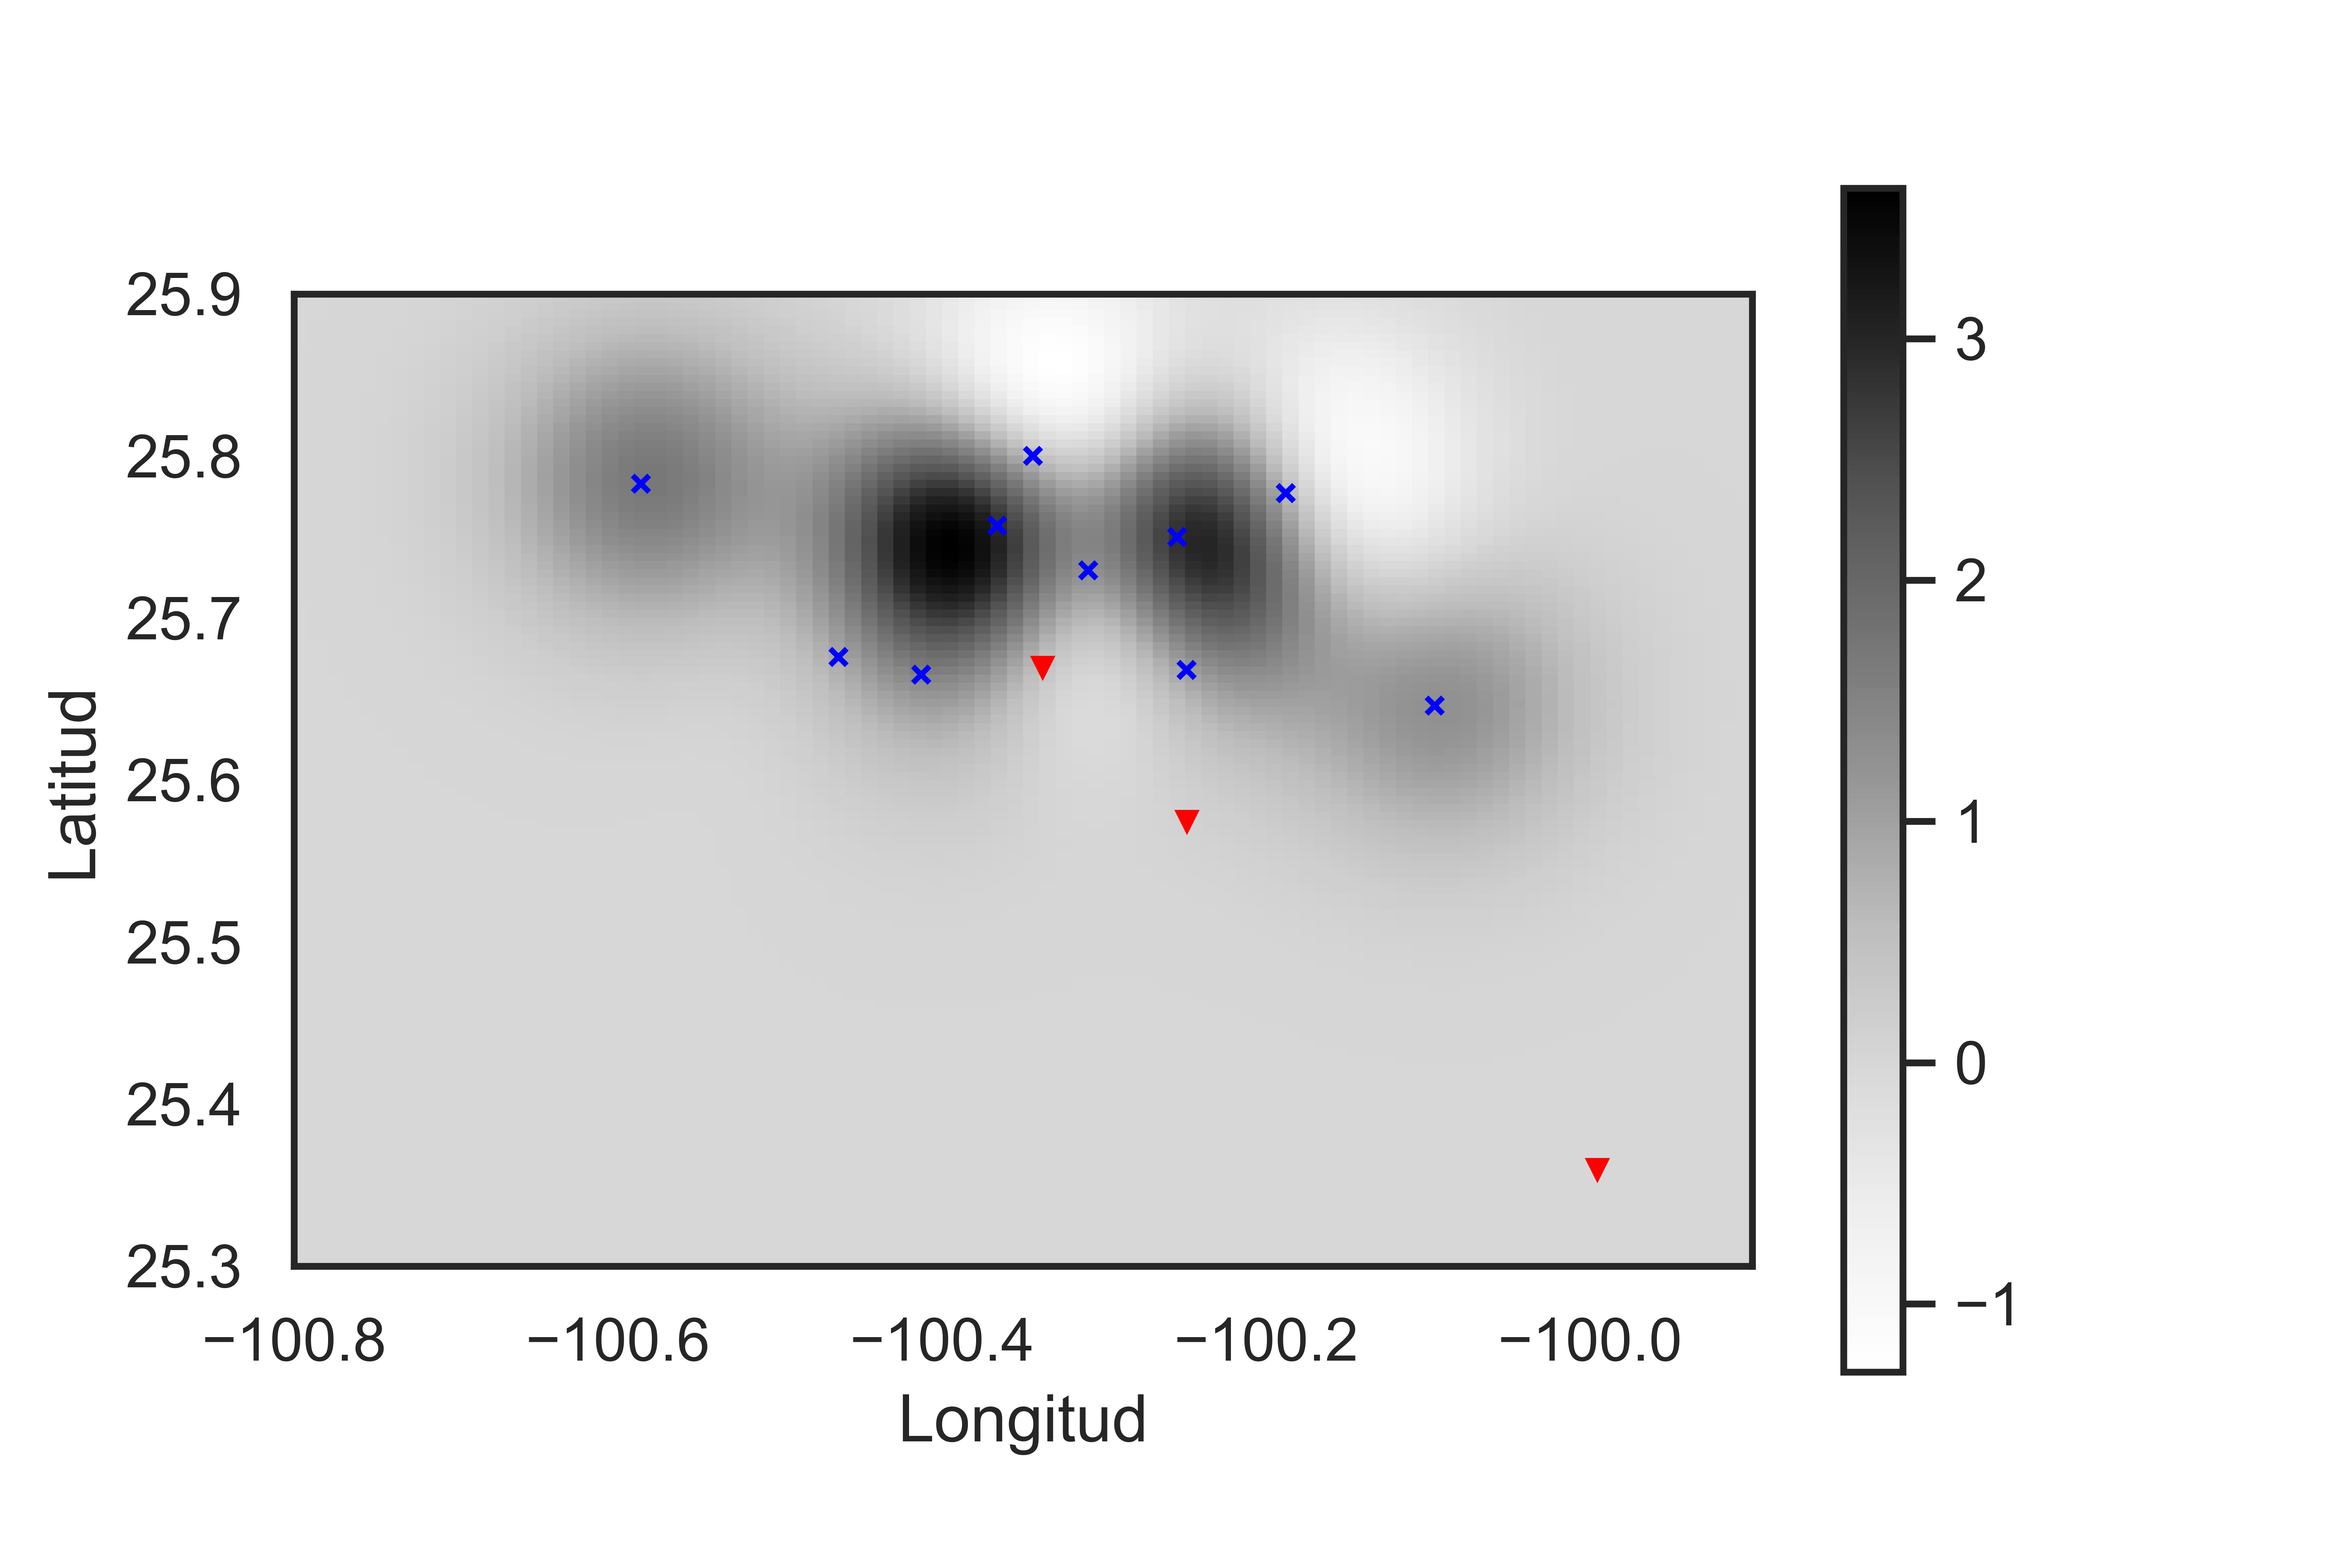
\includegraphics[width=4cm, height=4cm]{./brf_g_11_0_26302}}
\subfigure[FBR L] {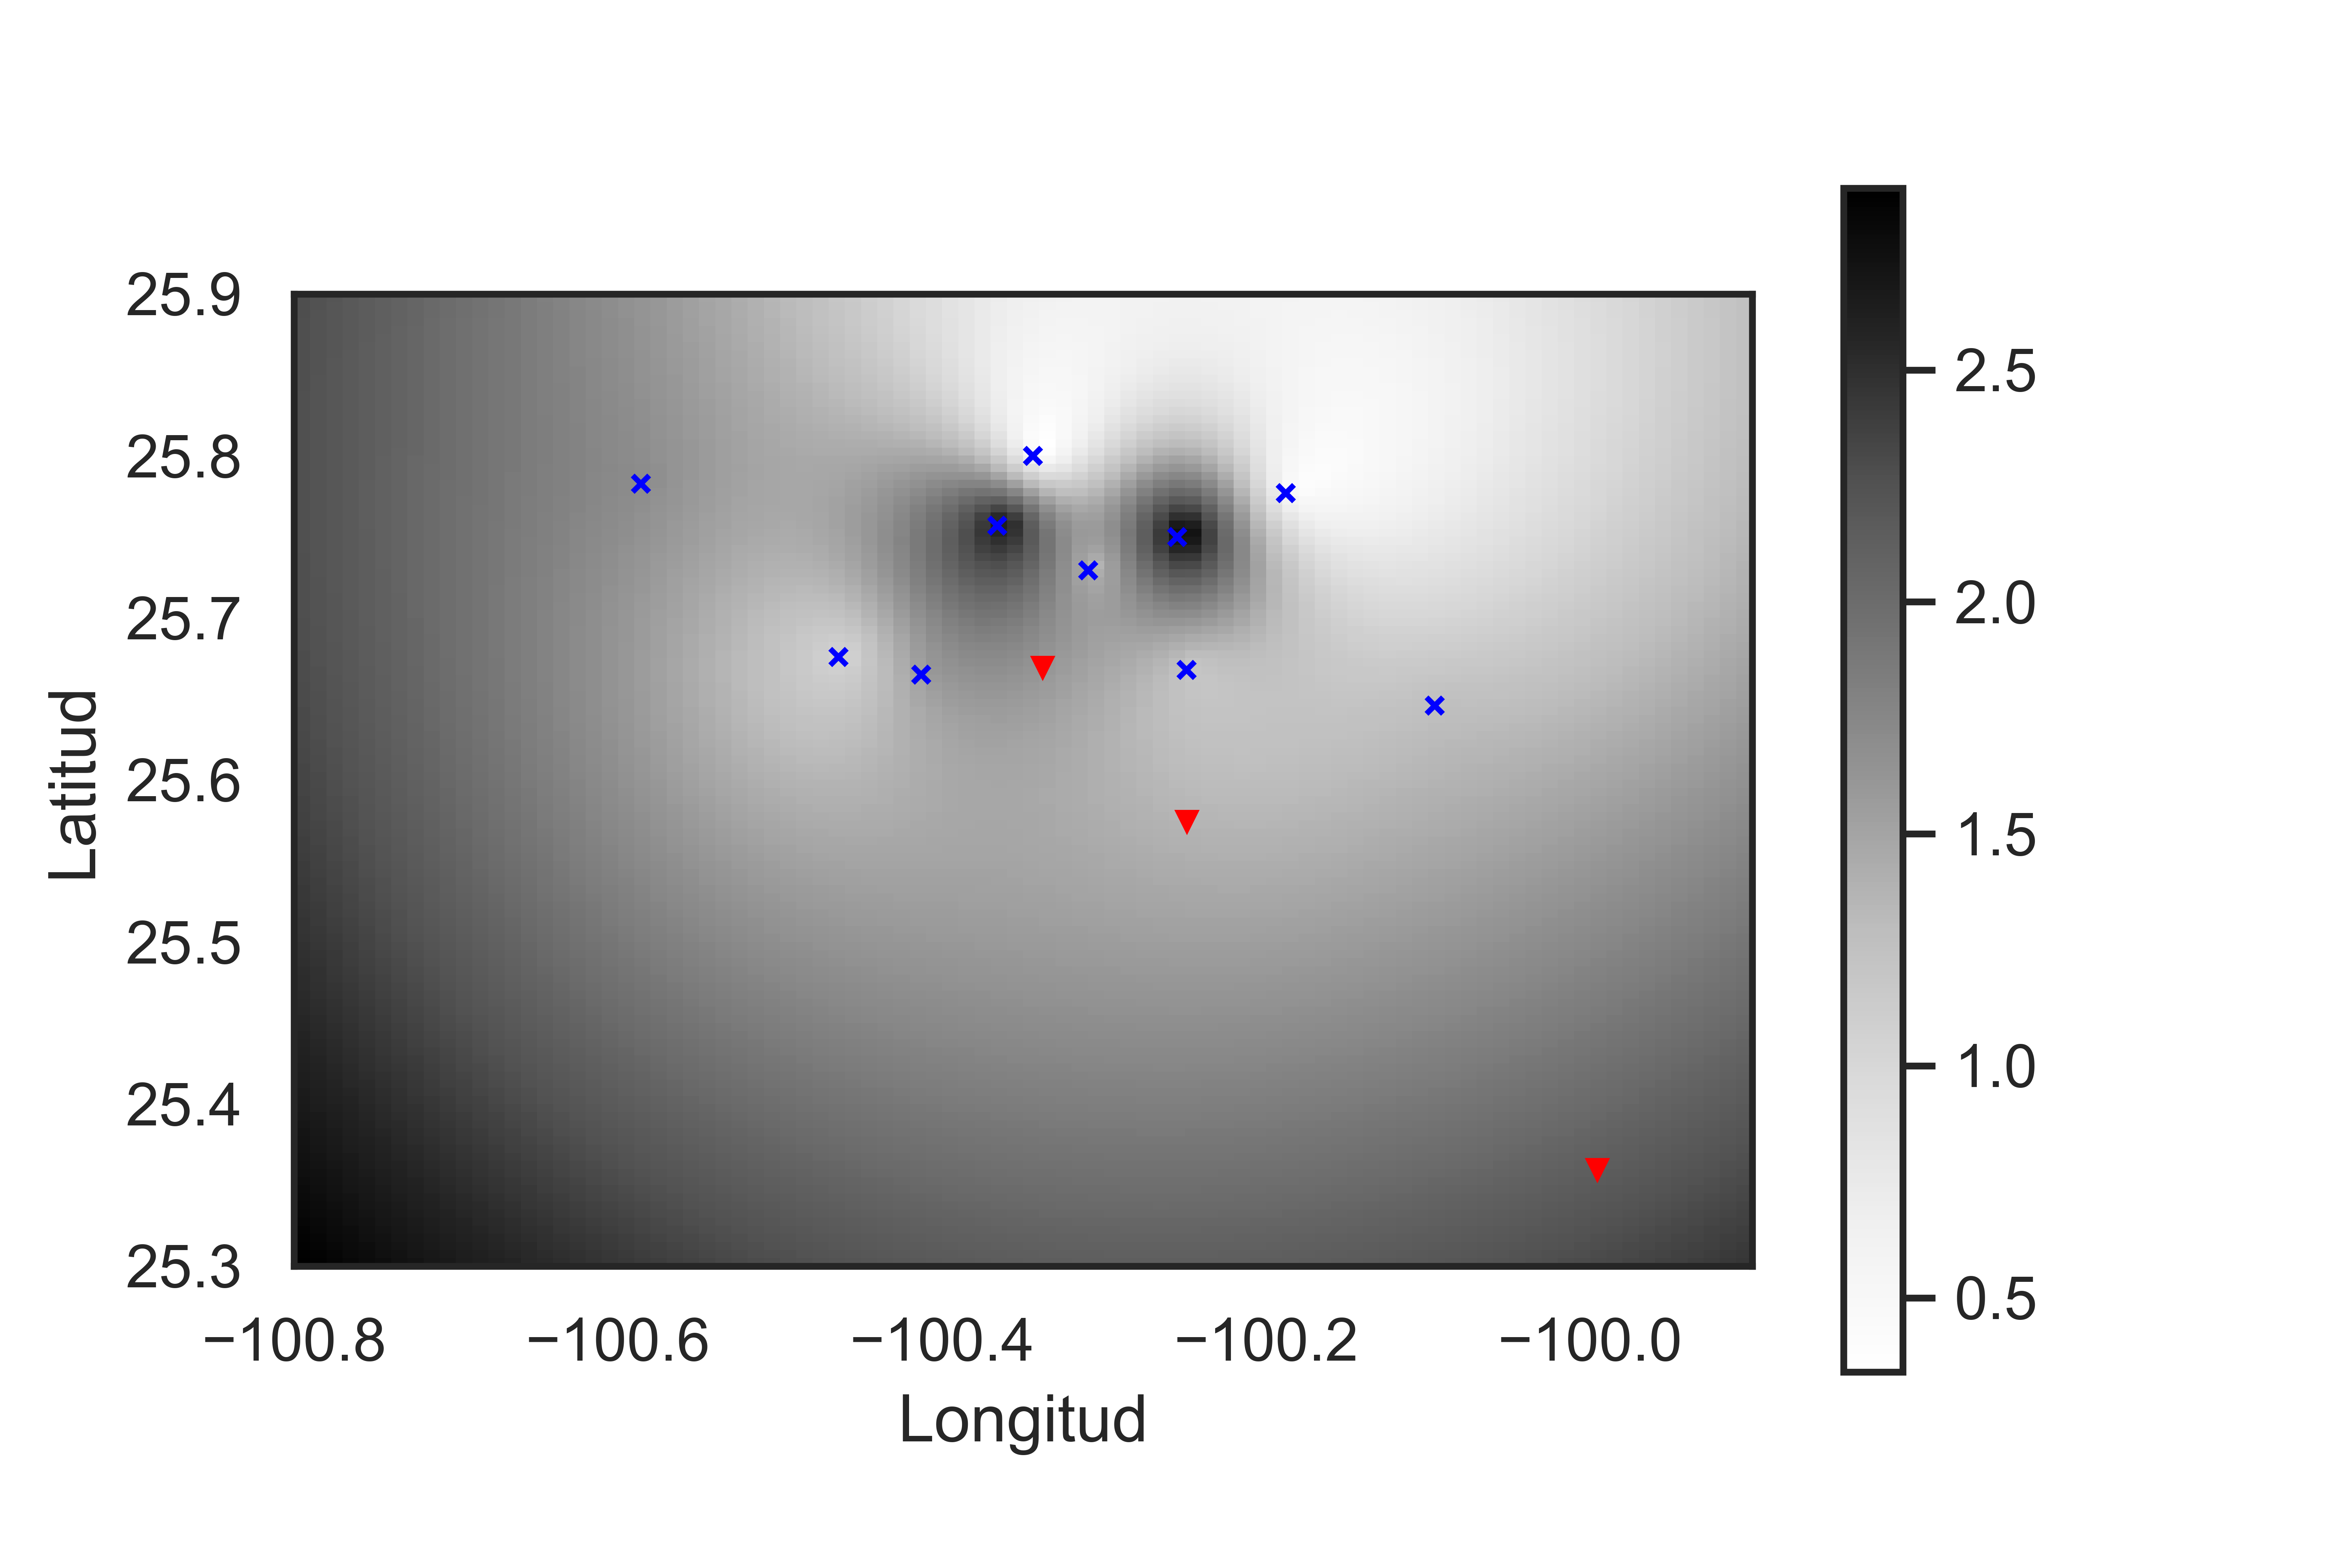
\includegraphics[width=4cm, height=4cm]{./brf_l_11_0_26302}}
\subfigure[FBR C] {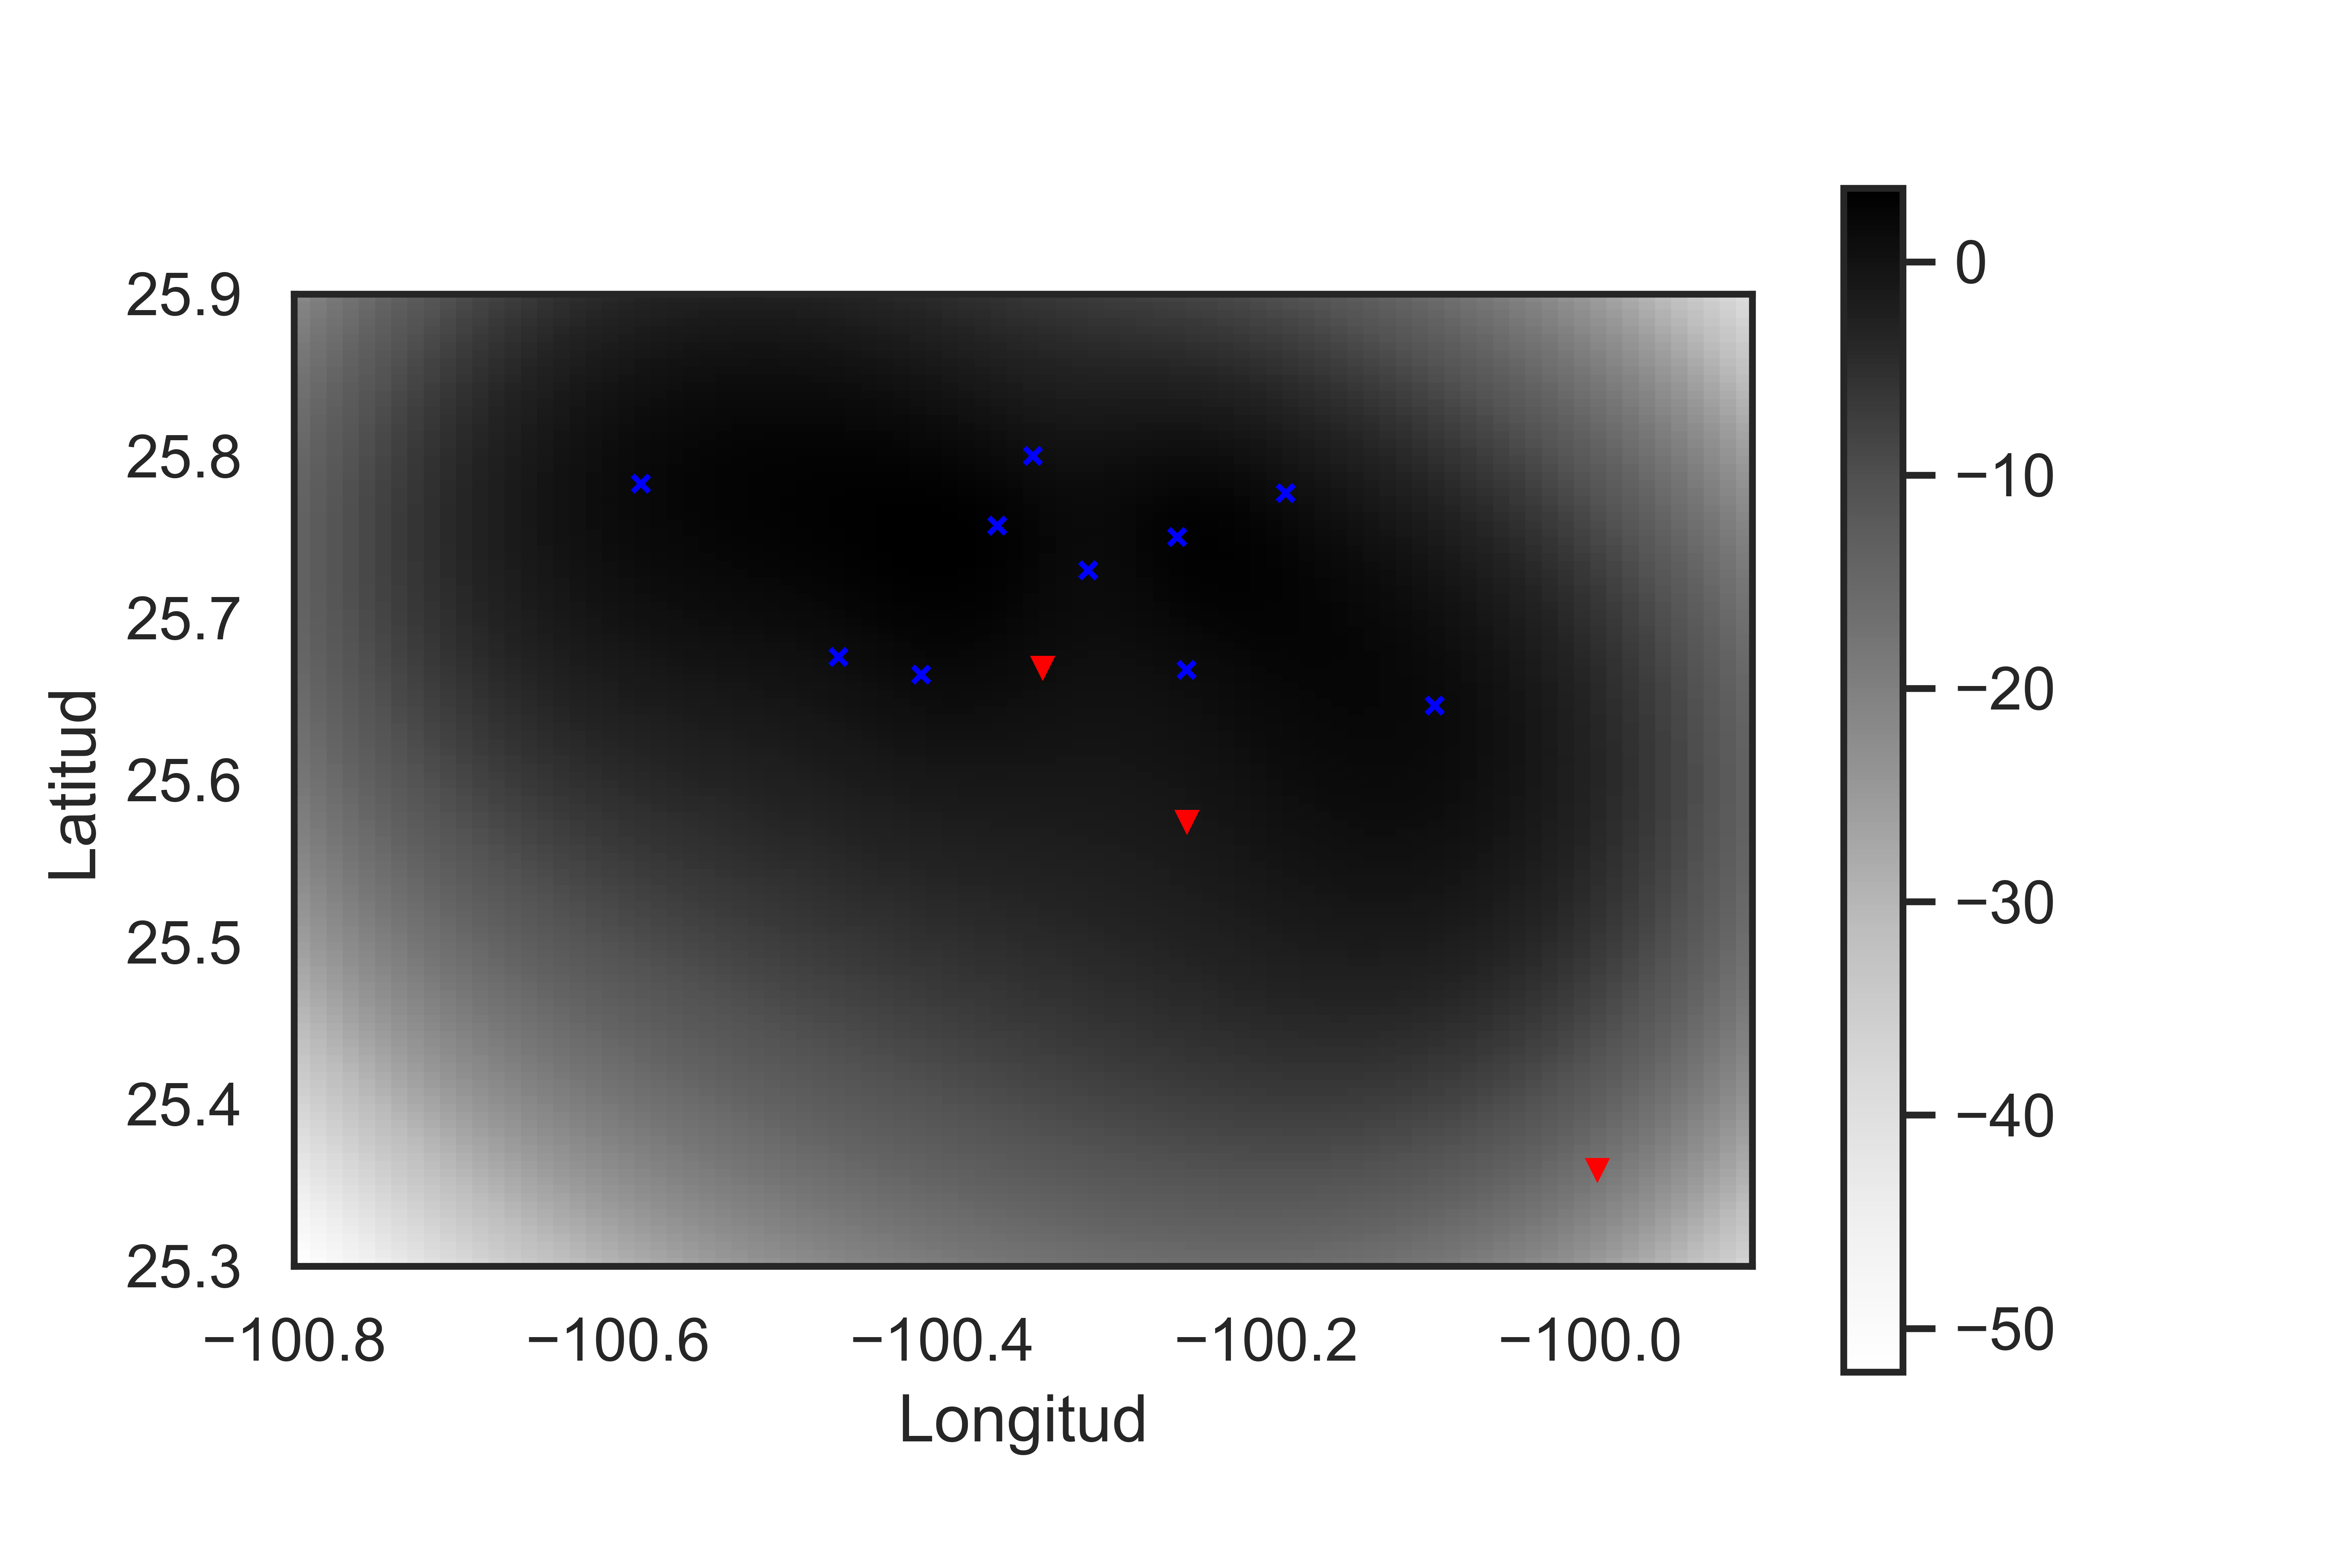
\includegraphics[width=4cm, height=4cm]{./brf_c_11_0_26302}}
\subfigure[FBR Q] {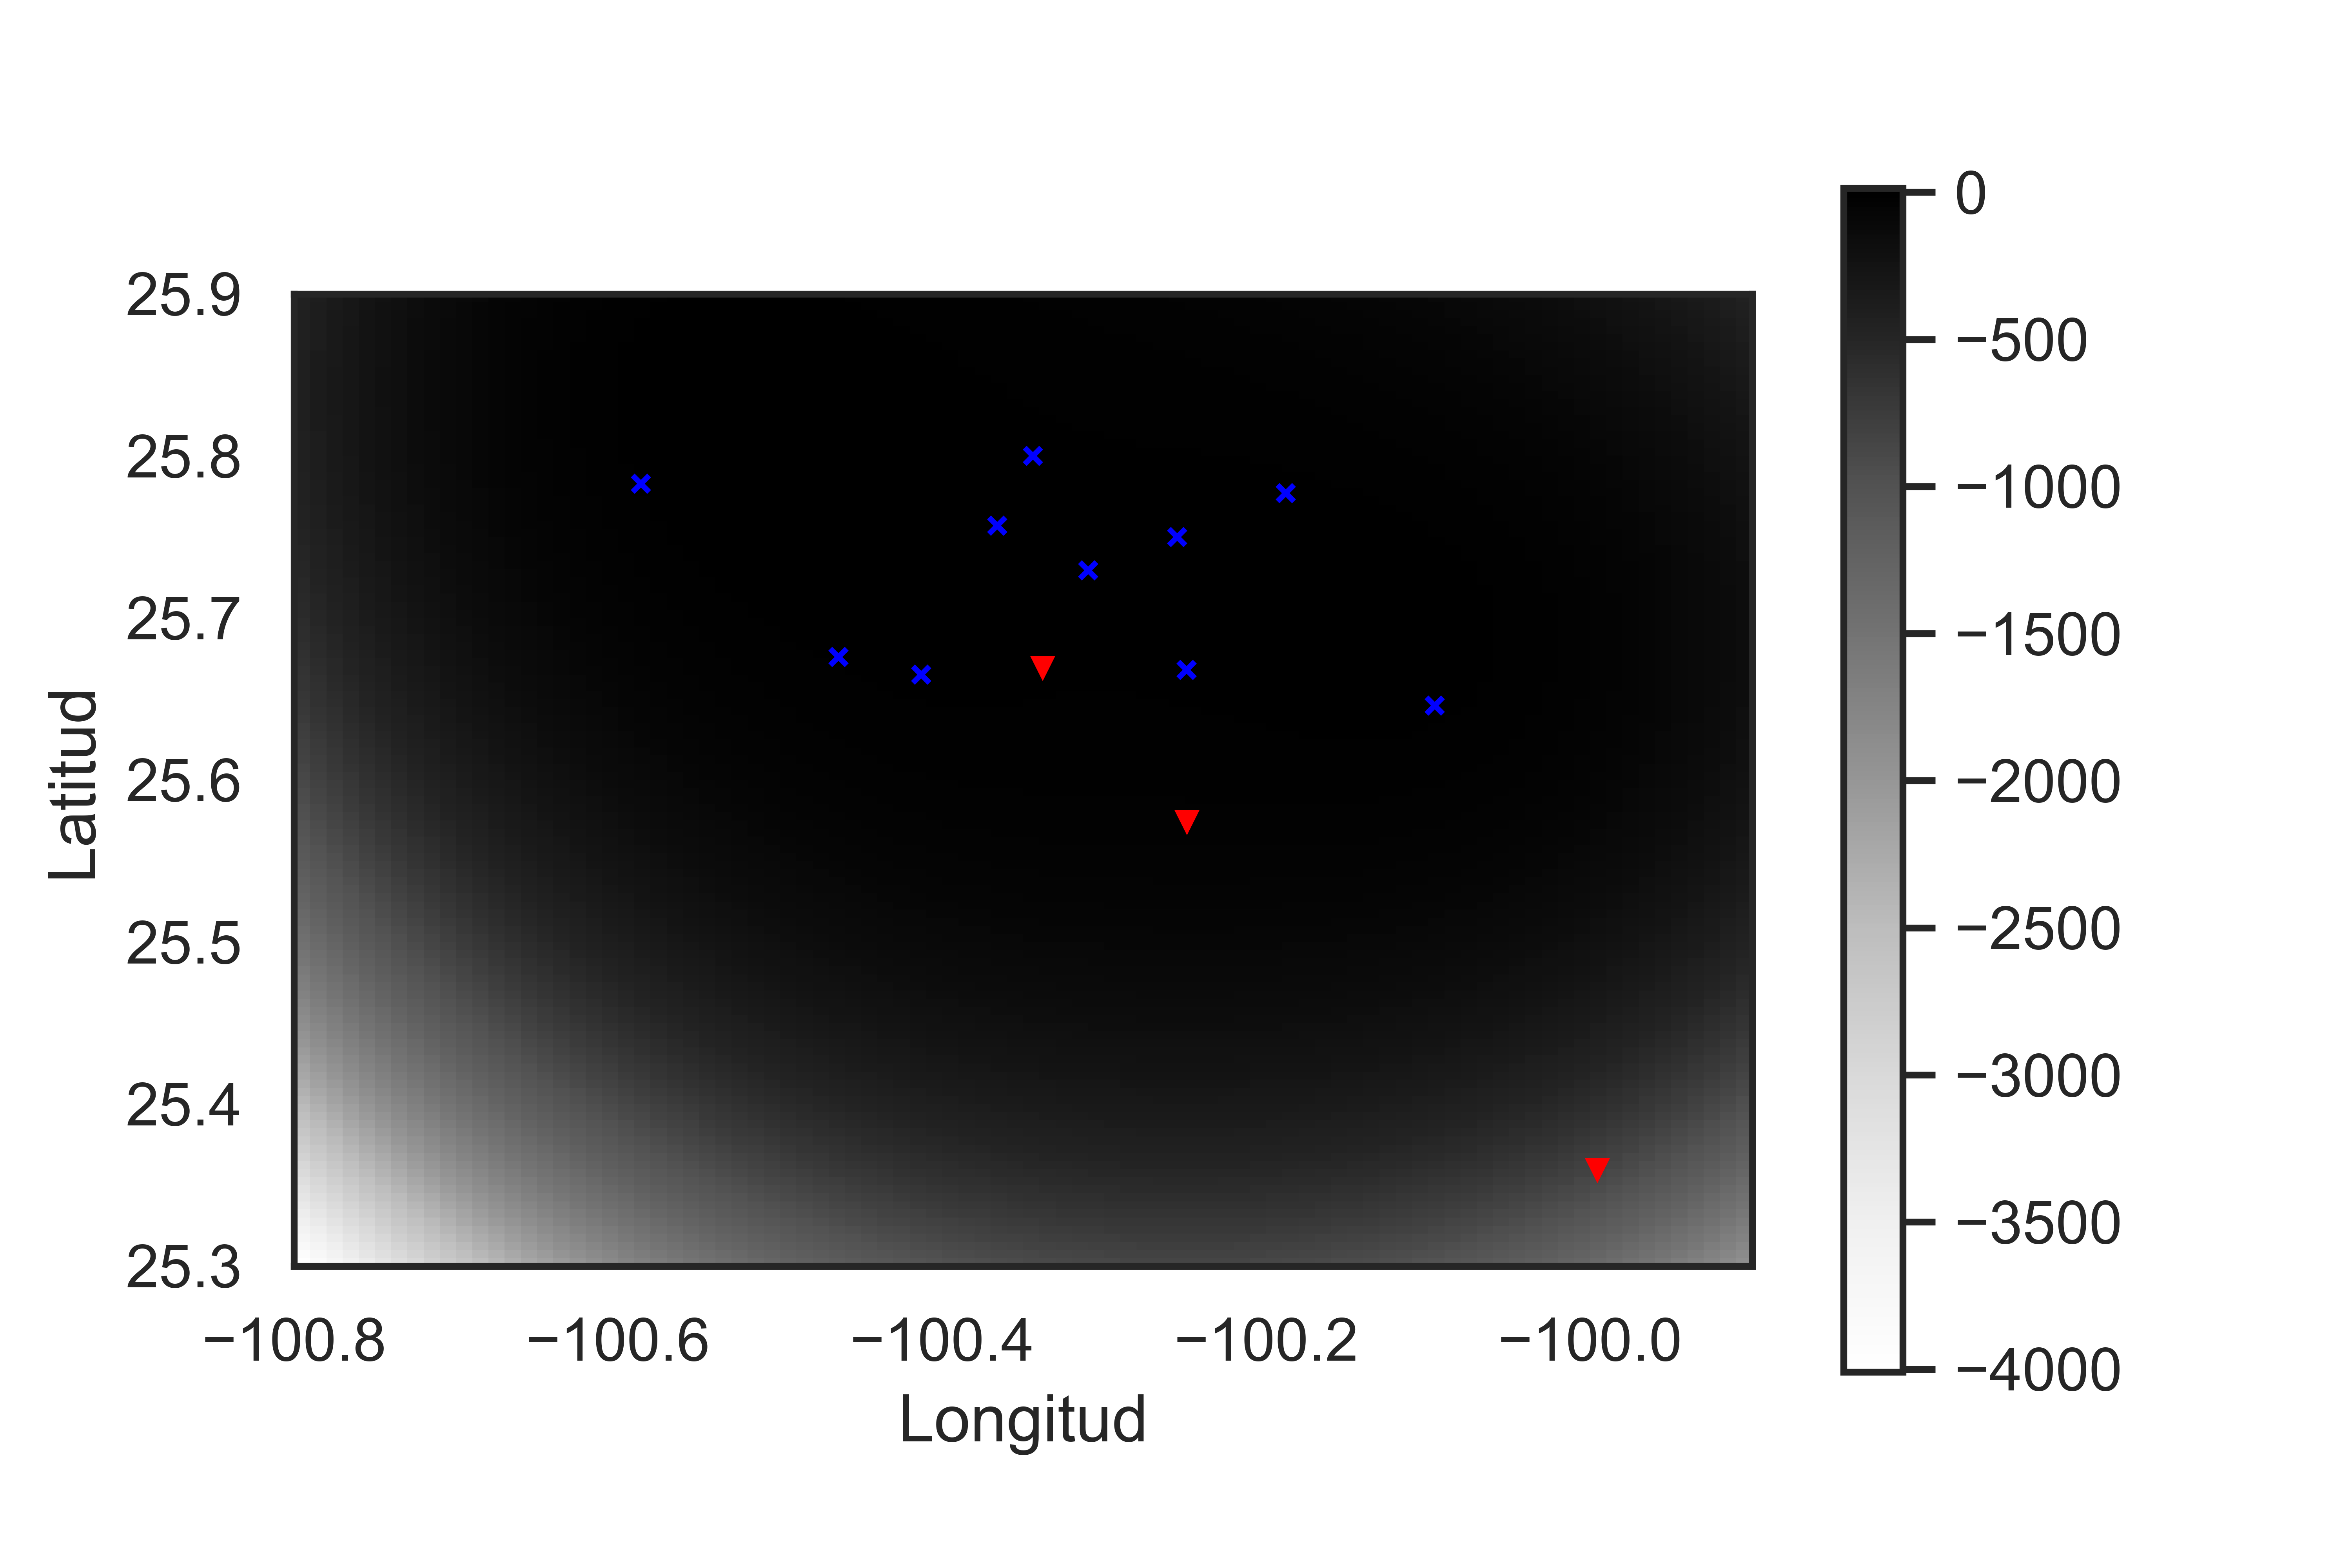
\includegraphics[width=4cm, height=4cm]{./brf_q_11_0_26302}}
\subfigure[FBR TPS] {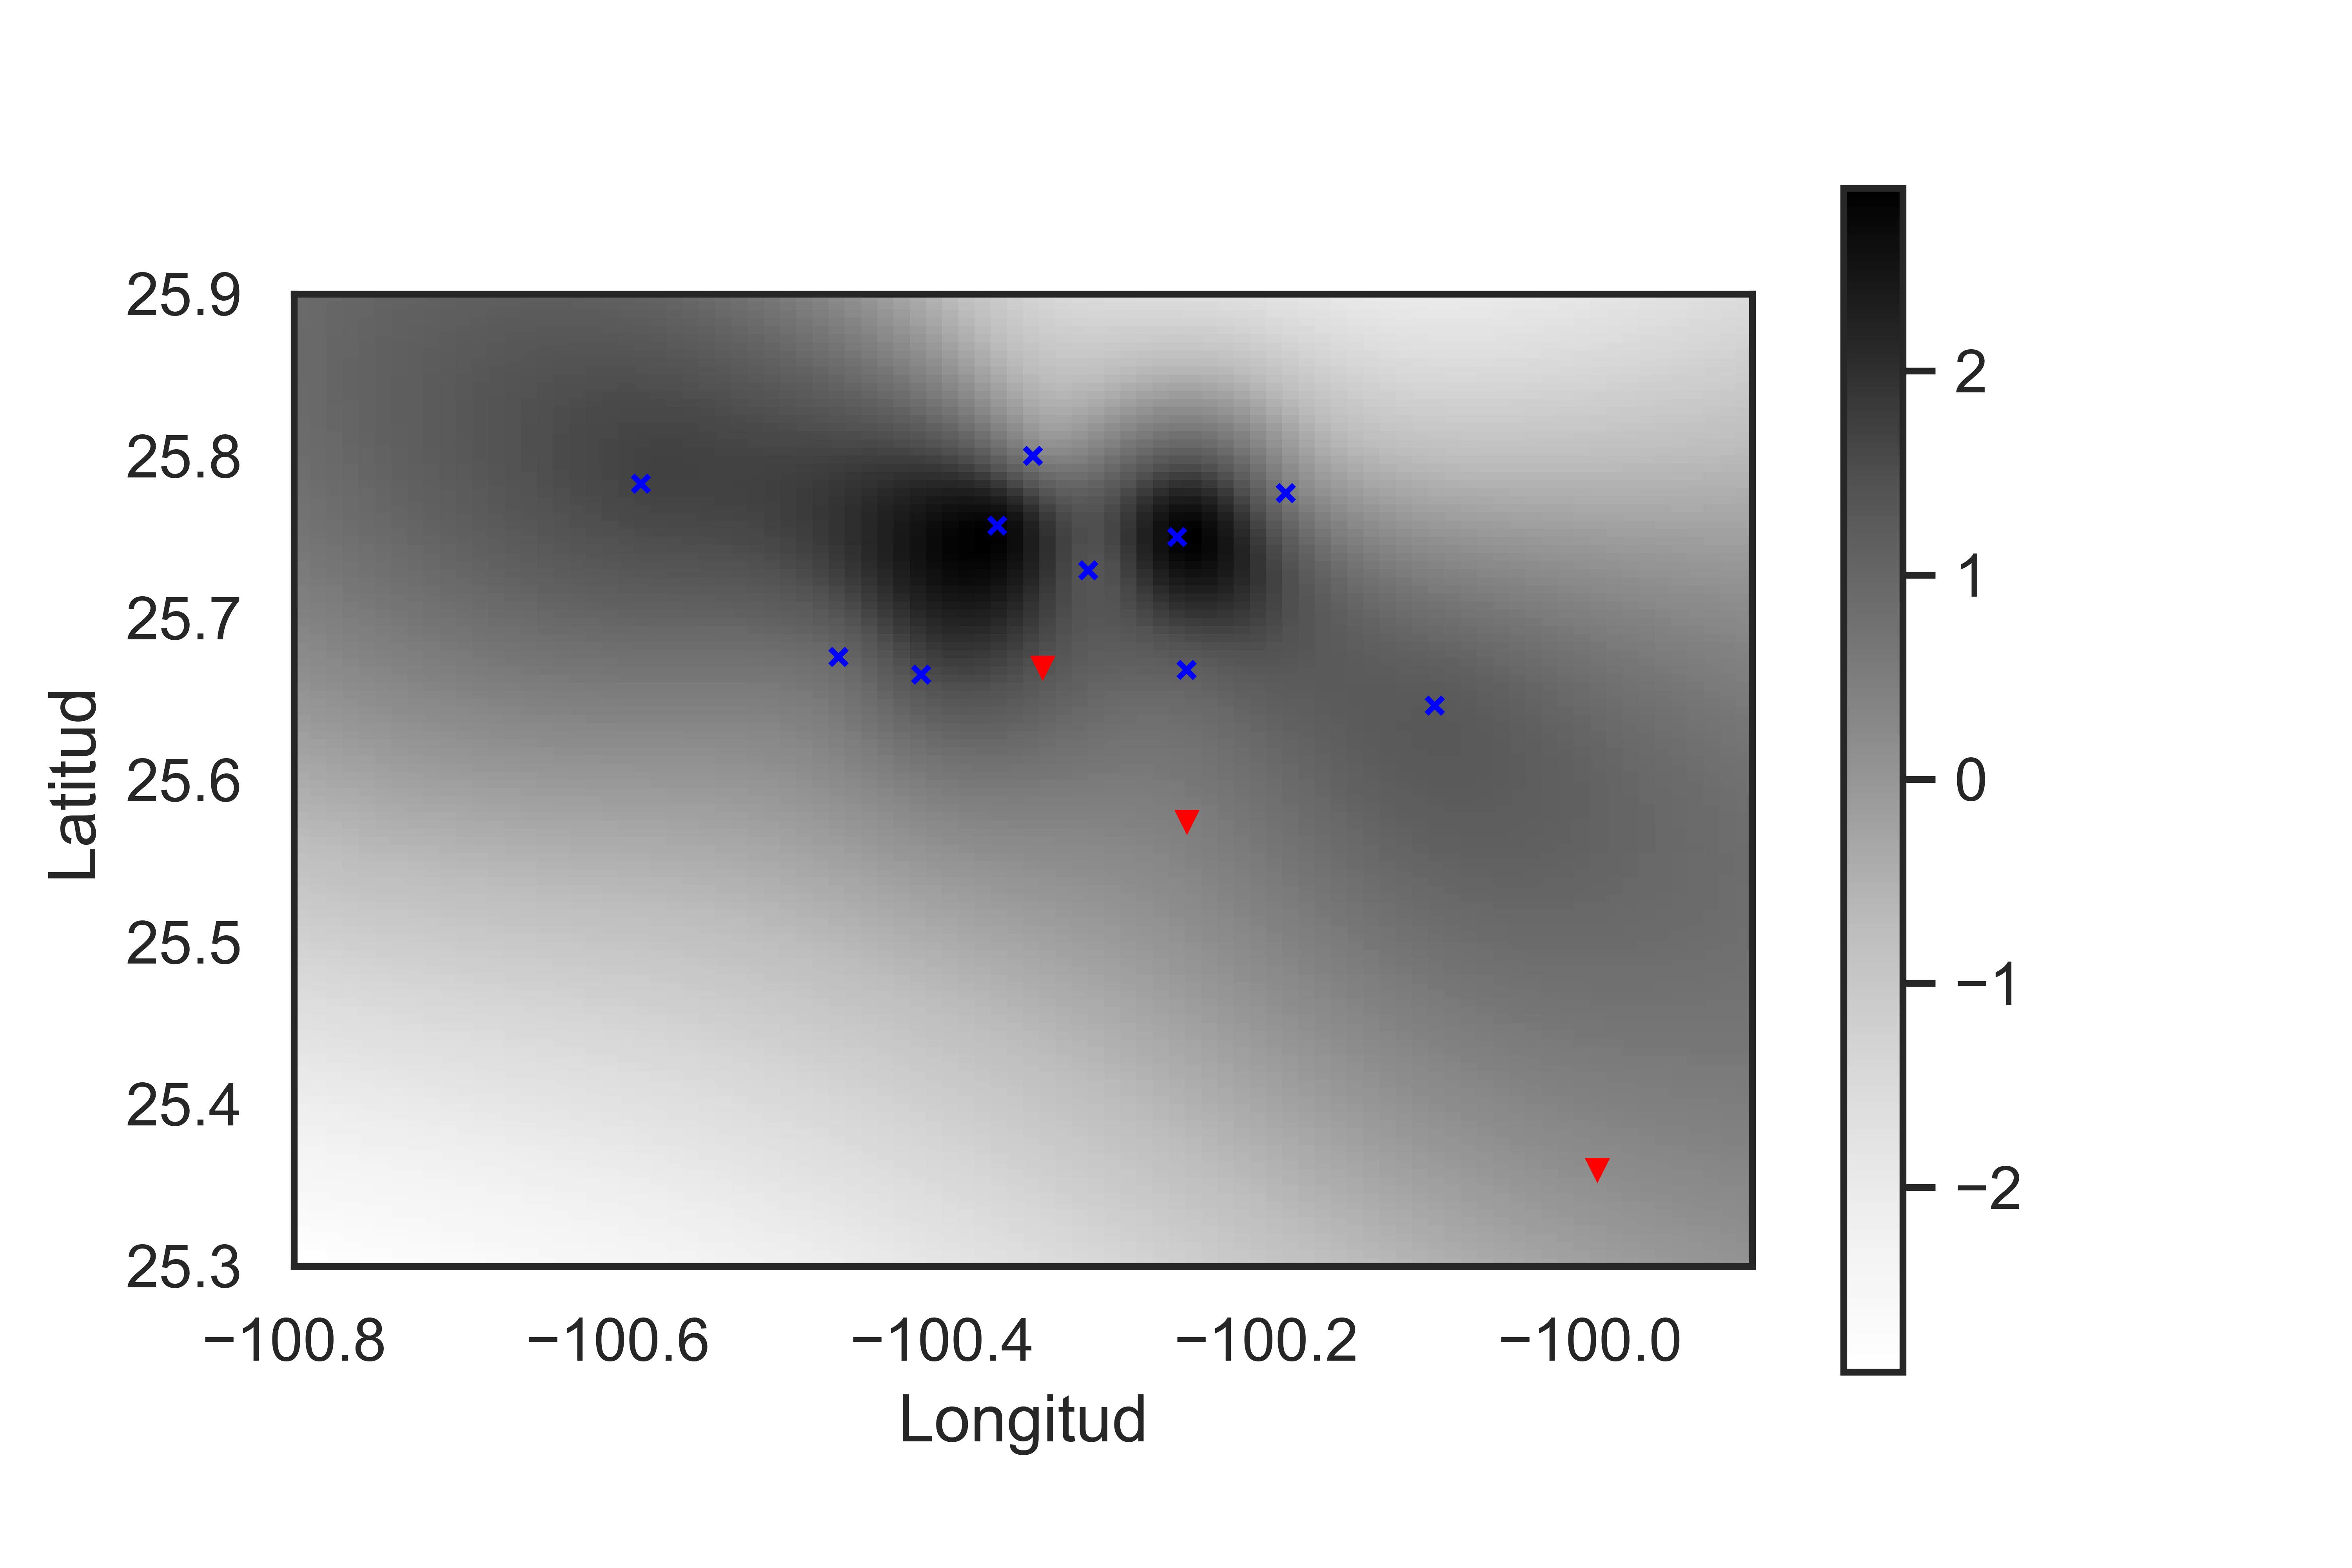
\includegraphics[width=4cm, height=4cm]{./brf_tps_11_0_26302}}
\subfigure[KO] {\includegraphics[width=4cm, height=4cm]{./ok_11_0_26302}}
\subfigure[KU] {\includegraphics[width=4cm, height=4cm]{./uk_11_0_26302}}
\caption{Interpolaciones de CO para 11 estaciones seleccionadas y 2 estaciones interpoladas: Fecha (31-12-2018 23:00:00)}
\label{COfigure3}
\end{figure}


\begin{table}[H]
\centering
\caption{CO: 12 estaciones seleccionadas 1 estación interpolada}
\begin{adjustbox}{max width=0.9\textwidth}
\begin{tabular}{|c|c|c|c|c|c|c|}
\hline
\multicolumn{7}{ |c| }{Métricas de error} \\ \hline
Método &MAPE &MAE &MAEP &RMSE &RMSEP &MSE \\ \hline
TV &1.04 &0.94 &0.70 &1.23 &0.92 &1.53 \\
DIP &0.87 &0.90 &0.67 &1.12 &0.84 &1.27 \\
FBR M &$2.20\times10^{17}$ &$3.29\times10^{17}$ &$2.46\times10^{17}$ &$1.74\times10^{18}$ &$1.30\times10^{18}$ &$3.04\times10^{36}$ \\
FBR IM &1.12 &1.14 &0.85 &1.60 &1.19 &2.56 \\
FBR G &$4.39\times10^{15}$ &$2.10\times10^{15}$ &$1.57\times10^{14}$ &$1.39\times10^{17}$ &$1.04\times10^{17}$ &$1.94\times10^{34}$ \\
FBR L &1.09 &1.03 &0.77 &1.34 &1.00 &1.80 \\
FBR C &$5.26\times10^{17}$ &$5.99\times10^{17}$ &$4.48\times10^{17}$ &$2.35\times10^{18}$ &$1.17\times10^{18}$ &$5.53\times10^{36}$ \\
FBR Q &$1.58\times10^{18}$ &$1.33\times10^{18}$ &$9.97\times10^{17}$ &$3.50\times10^{18}$ &$2.62\times10^{18}$ &$1.23\times10^{37}$ \\
FBR TPS &1.31 &1.22 &0.91 &1.70 &1.27 &2.90 \\
KO &0.84 &0.88 &0.66 &1.11 &0.83 &1.24 \\
KU &1.07 &0.98 &0.73 &1.32 &0.99 &1.76 \\\hline
\end{tabular}
\end{adjustbox}
\label{tabCO_4}
\end{table}


De la tabla \ref{tabCO_4}, en la cual se utilizan doce estaciones para interpolar una estación, podemos ver que los métodos que obtiene peores resultados de predicción son los métodos de Funciones de Base Radial, a excepción de los métodos inverso multicuadrático, lineal y {\em thin plate splines} (FBR I,  FBR L y FBR TPS), entre los métodos deterministas, el método DIP obtuvo el menor MAPE, MAE, MAEP, RMSE, RMSEP y MSE; mientras que de los métodos geoestadísticos el método KO obtuvo el menor MAPE, MAE, MAEP, RMSE, RMSEP y MSE. Los métodos DIP y KO son mejores que el resto de los métodos pero KO es mejor que DIP ya que en todos los errores son menores o igual a los errores de DIP. En la figura \ref{COfigure4}, se pueden observar las interpolaciones de cada método, donde las puntos azules son las estaciones seleccionadas y los puntos rojos son las estaciones interpoladas. En general, mientras se aumenta el número de estaciones para interpolar la variable CO, éstas bajan de forma rápida sus errores en algunos métodos como las Funciones de Base Radial y para el resto de los métodos que ya son buenos para interpolar también mejoran pero los cambios suceden con menor intensidad.


\begin{figure}[H]
\centering
\subfigure[TV] {\includegraphics[width=4cm, height=4cm]{./voronoi_12_0_26302}}
\subfigure[DIP] {\includegraphics[width=4cm, height=4cm]{./idw_12_0_26302}}
\subfigure[FBR M] {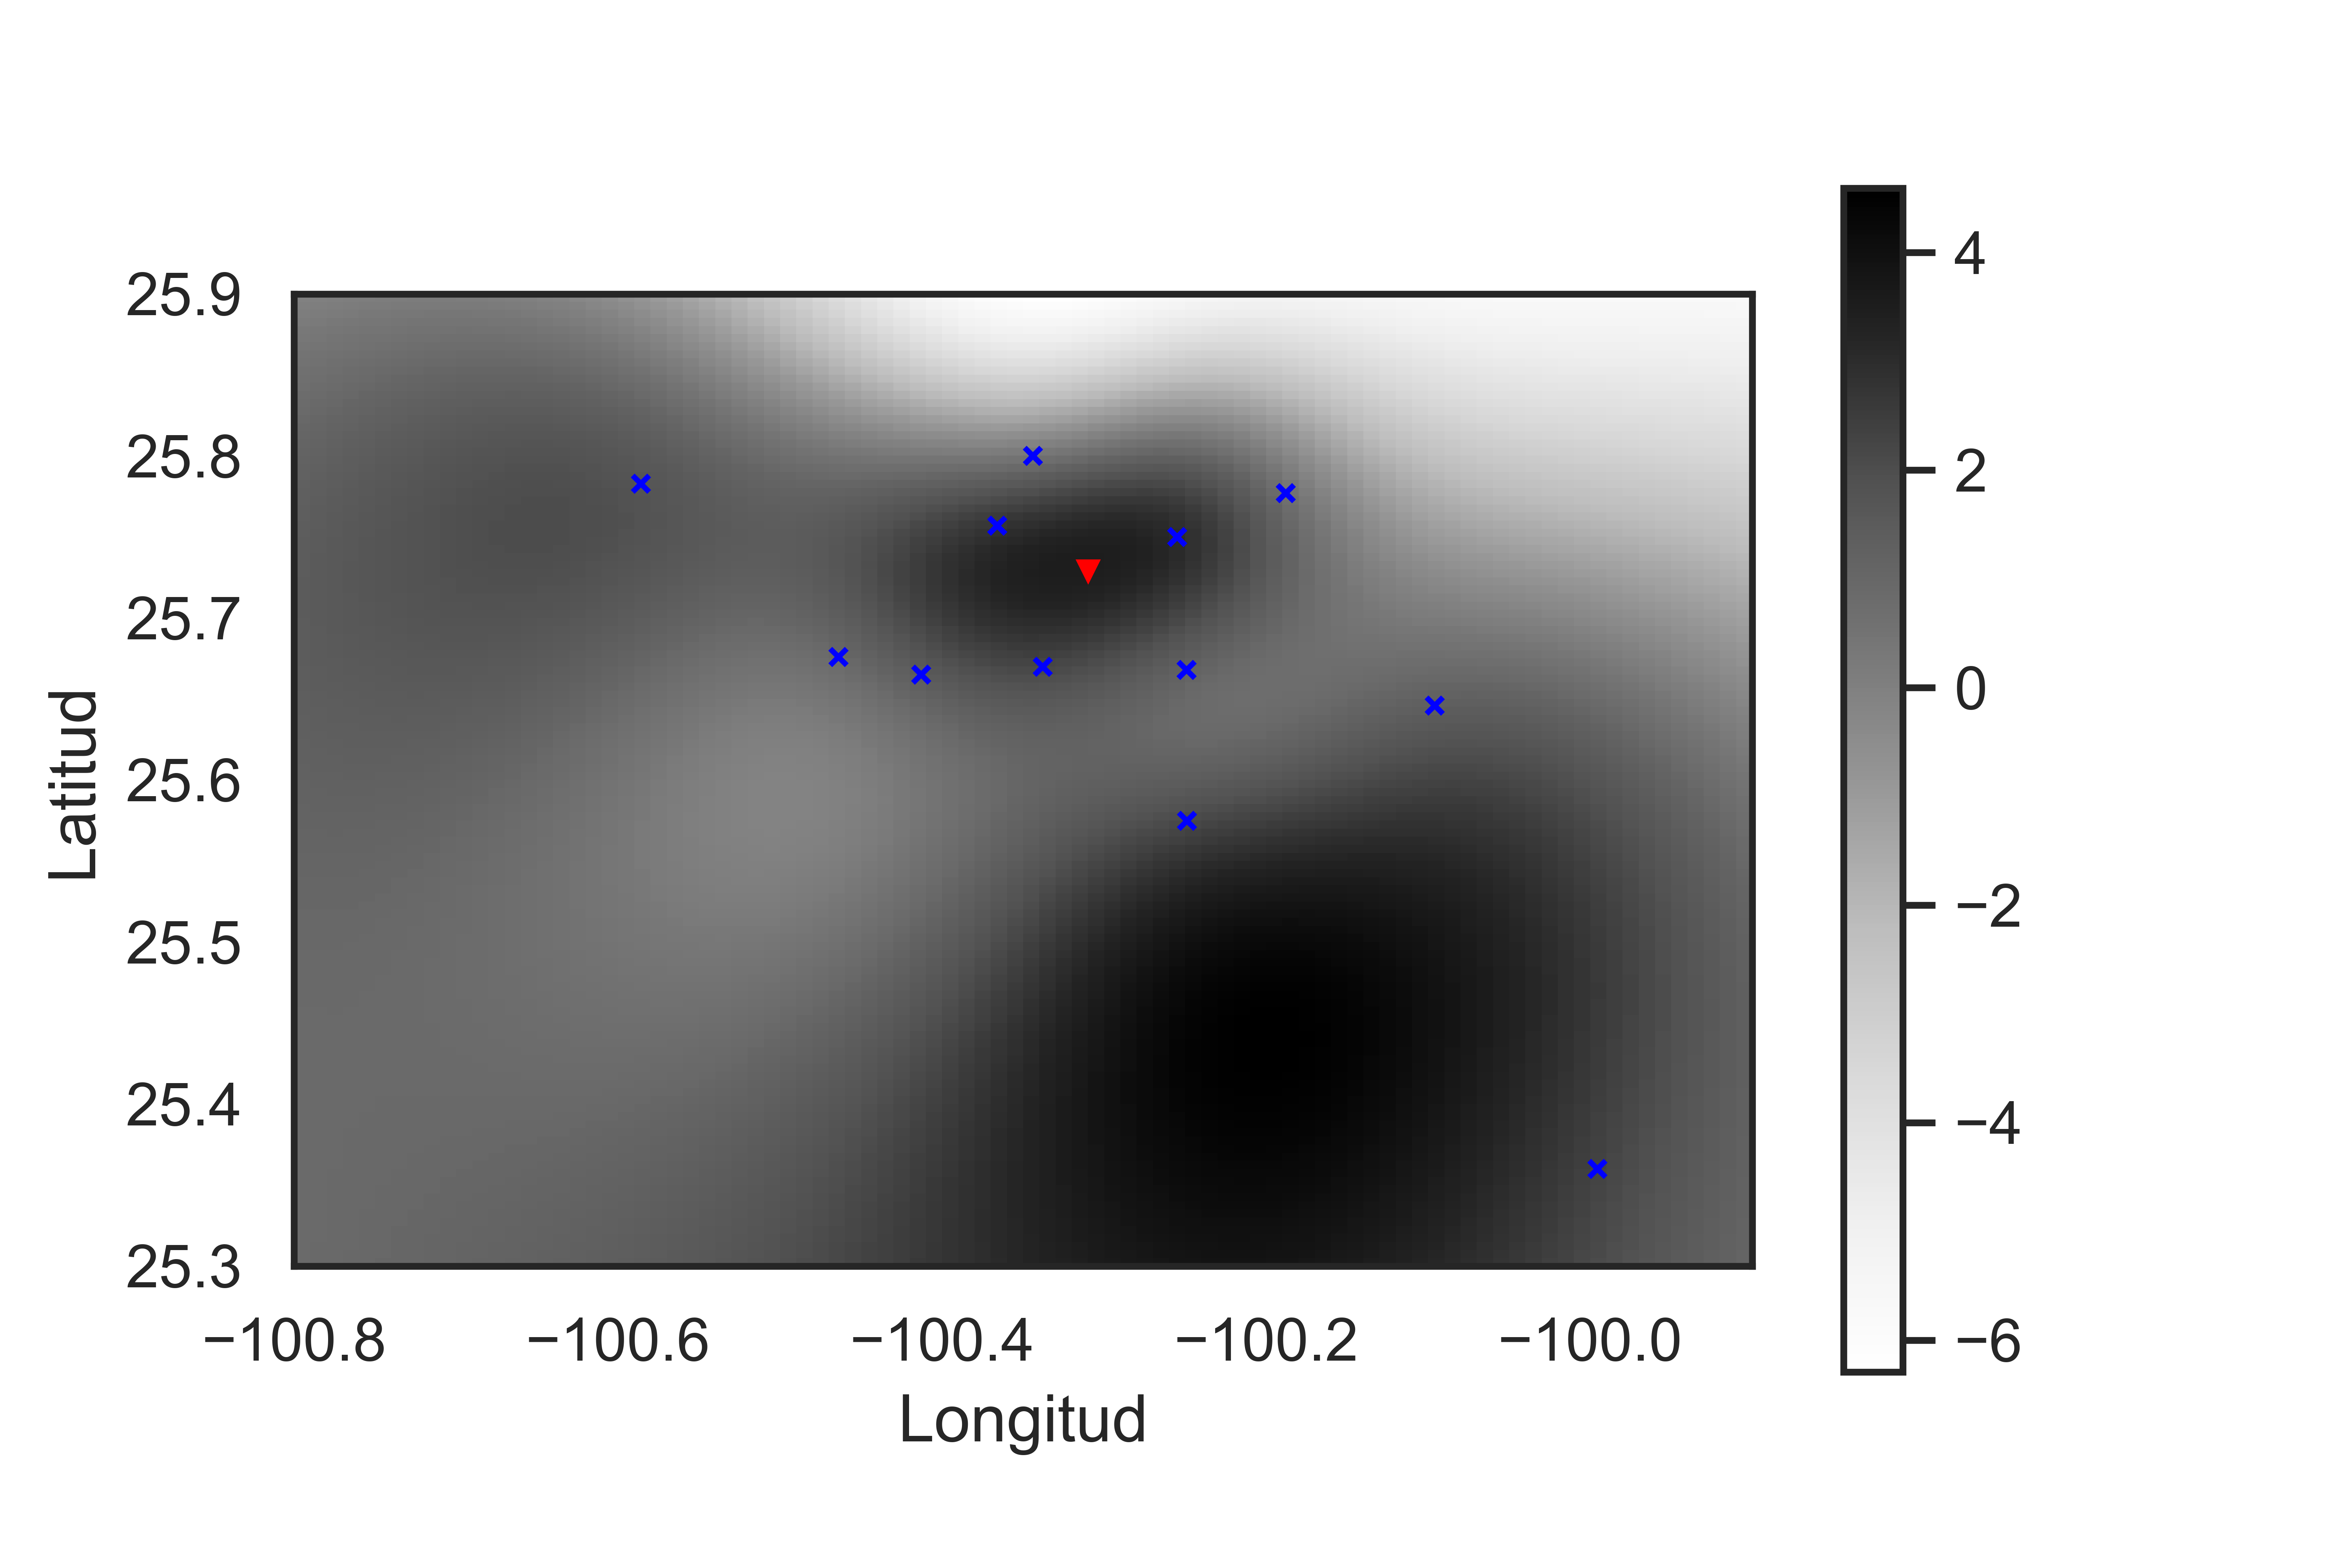
\includegraphics[width=4cm, height=4cm]{./brf_m_12_0_26302}}
\subfigure[FBR I] {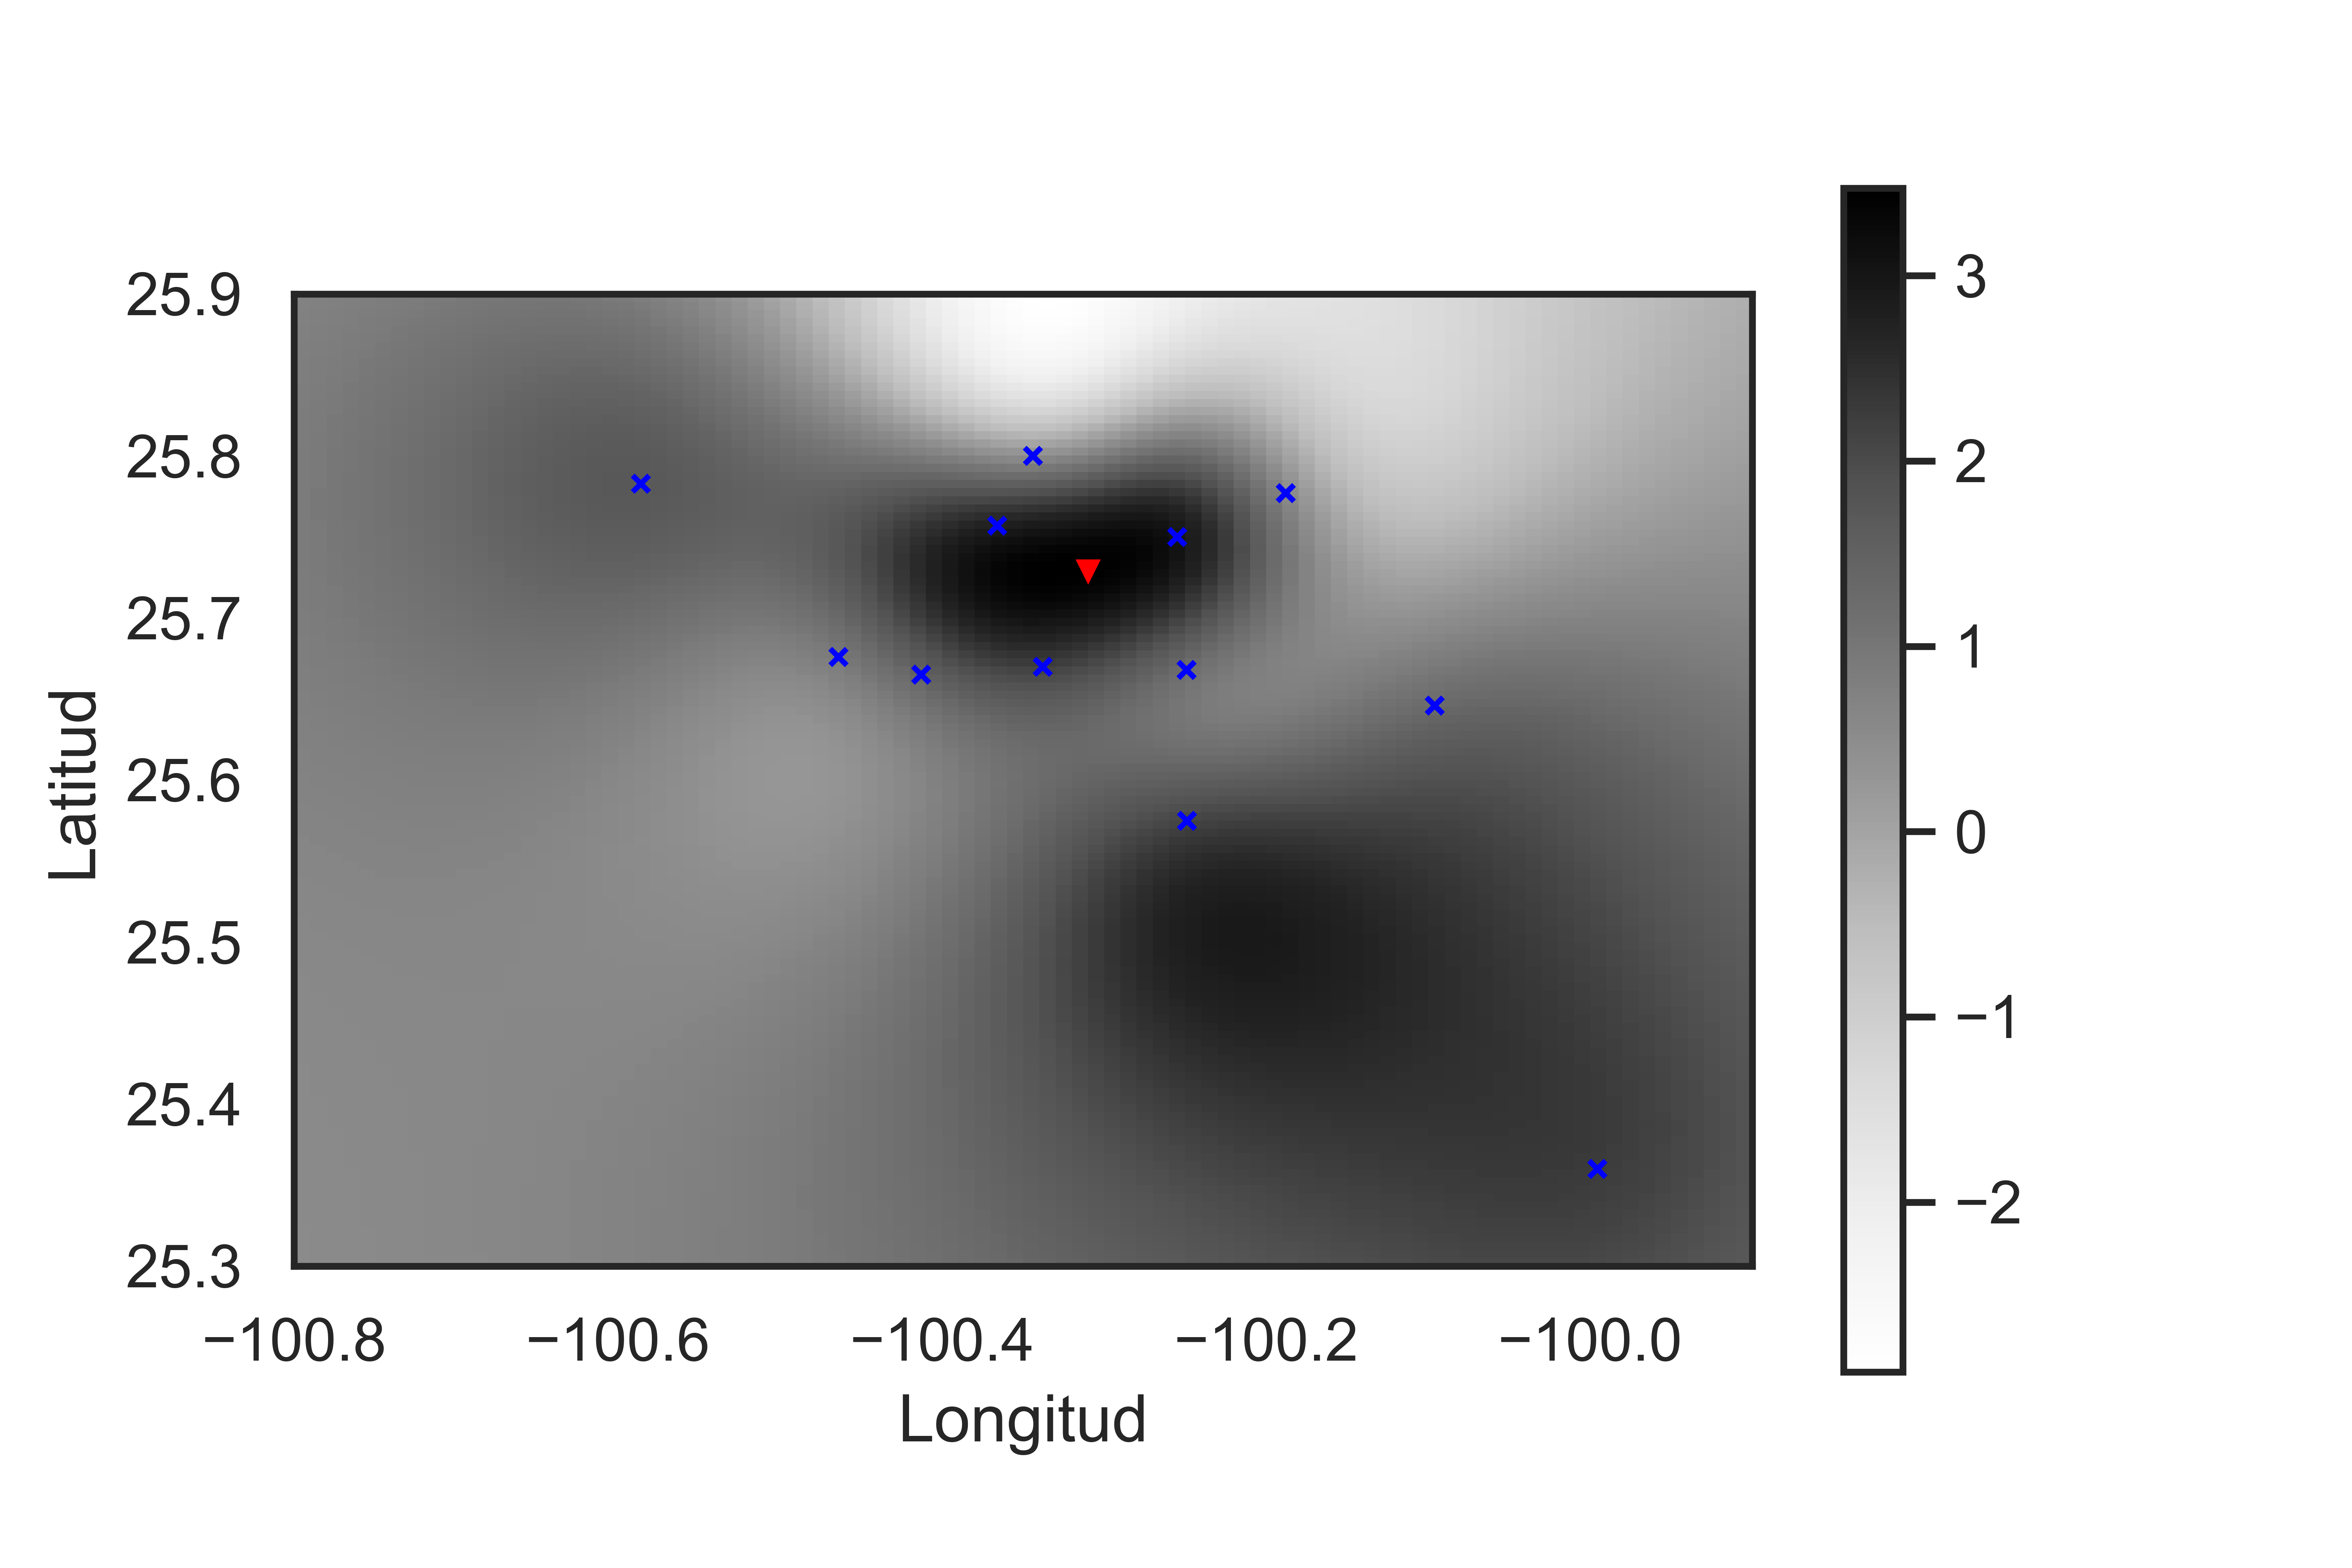
\includegraphics[width=4cm, height=4cm]{./brf_i_12_0_26302}}
\subfigure[FBR G] {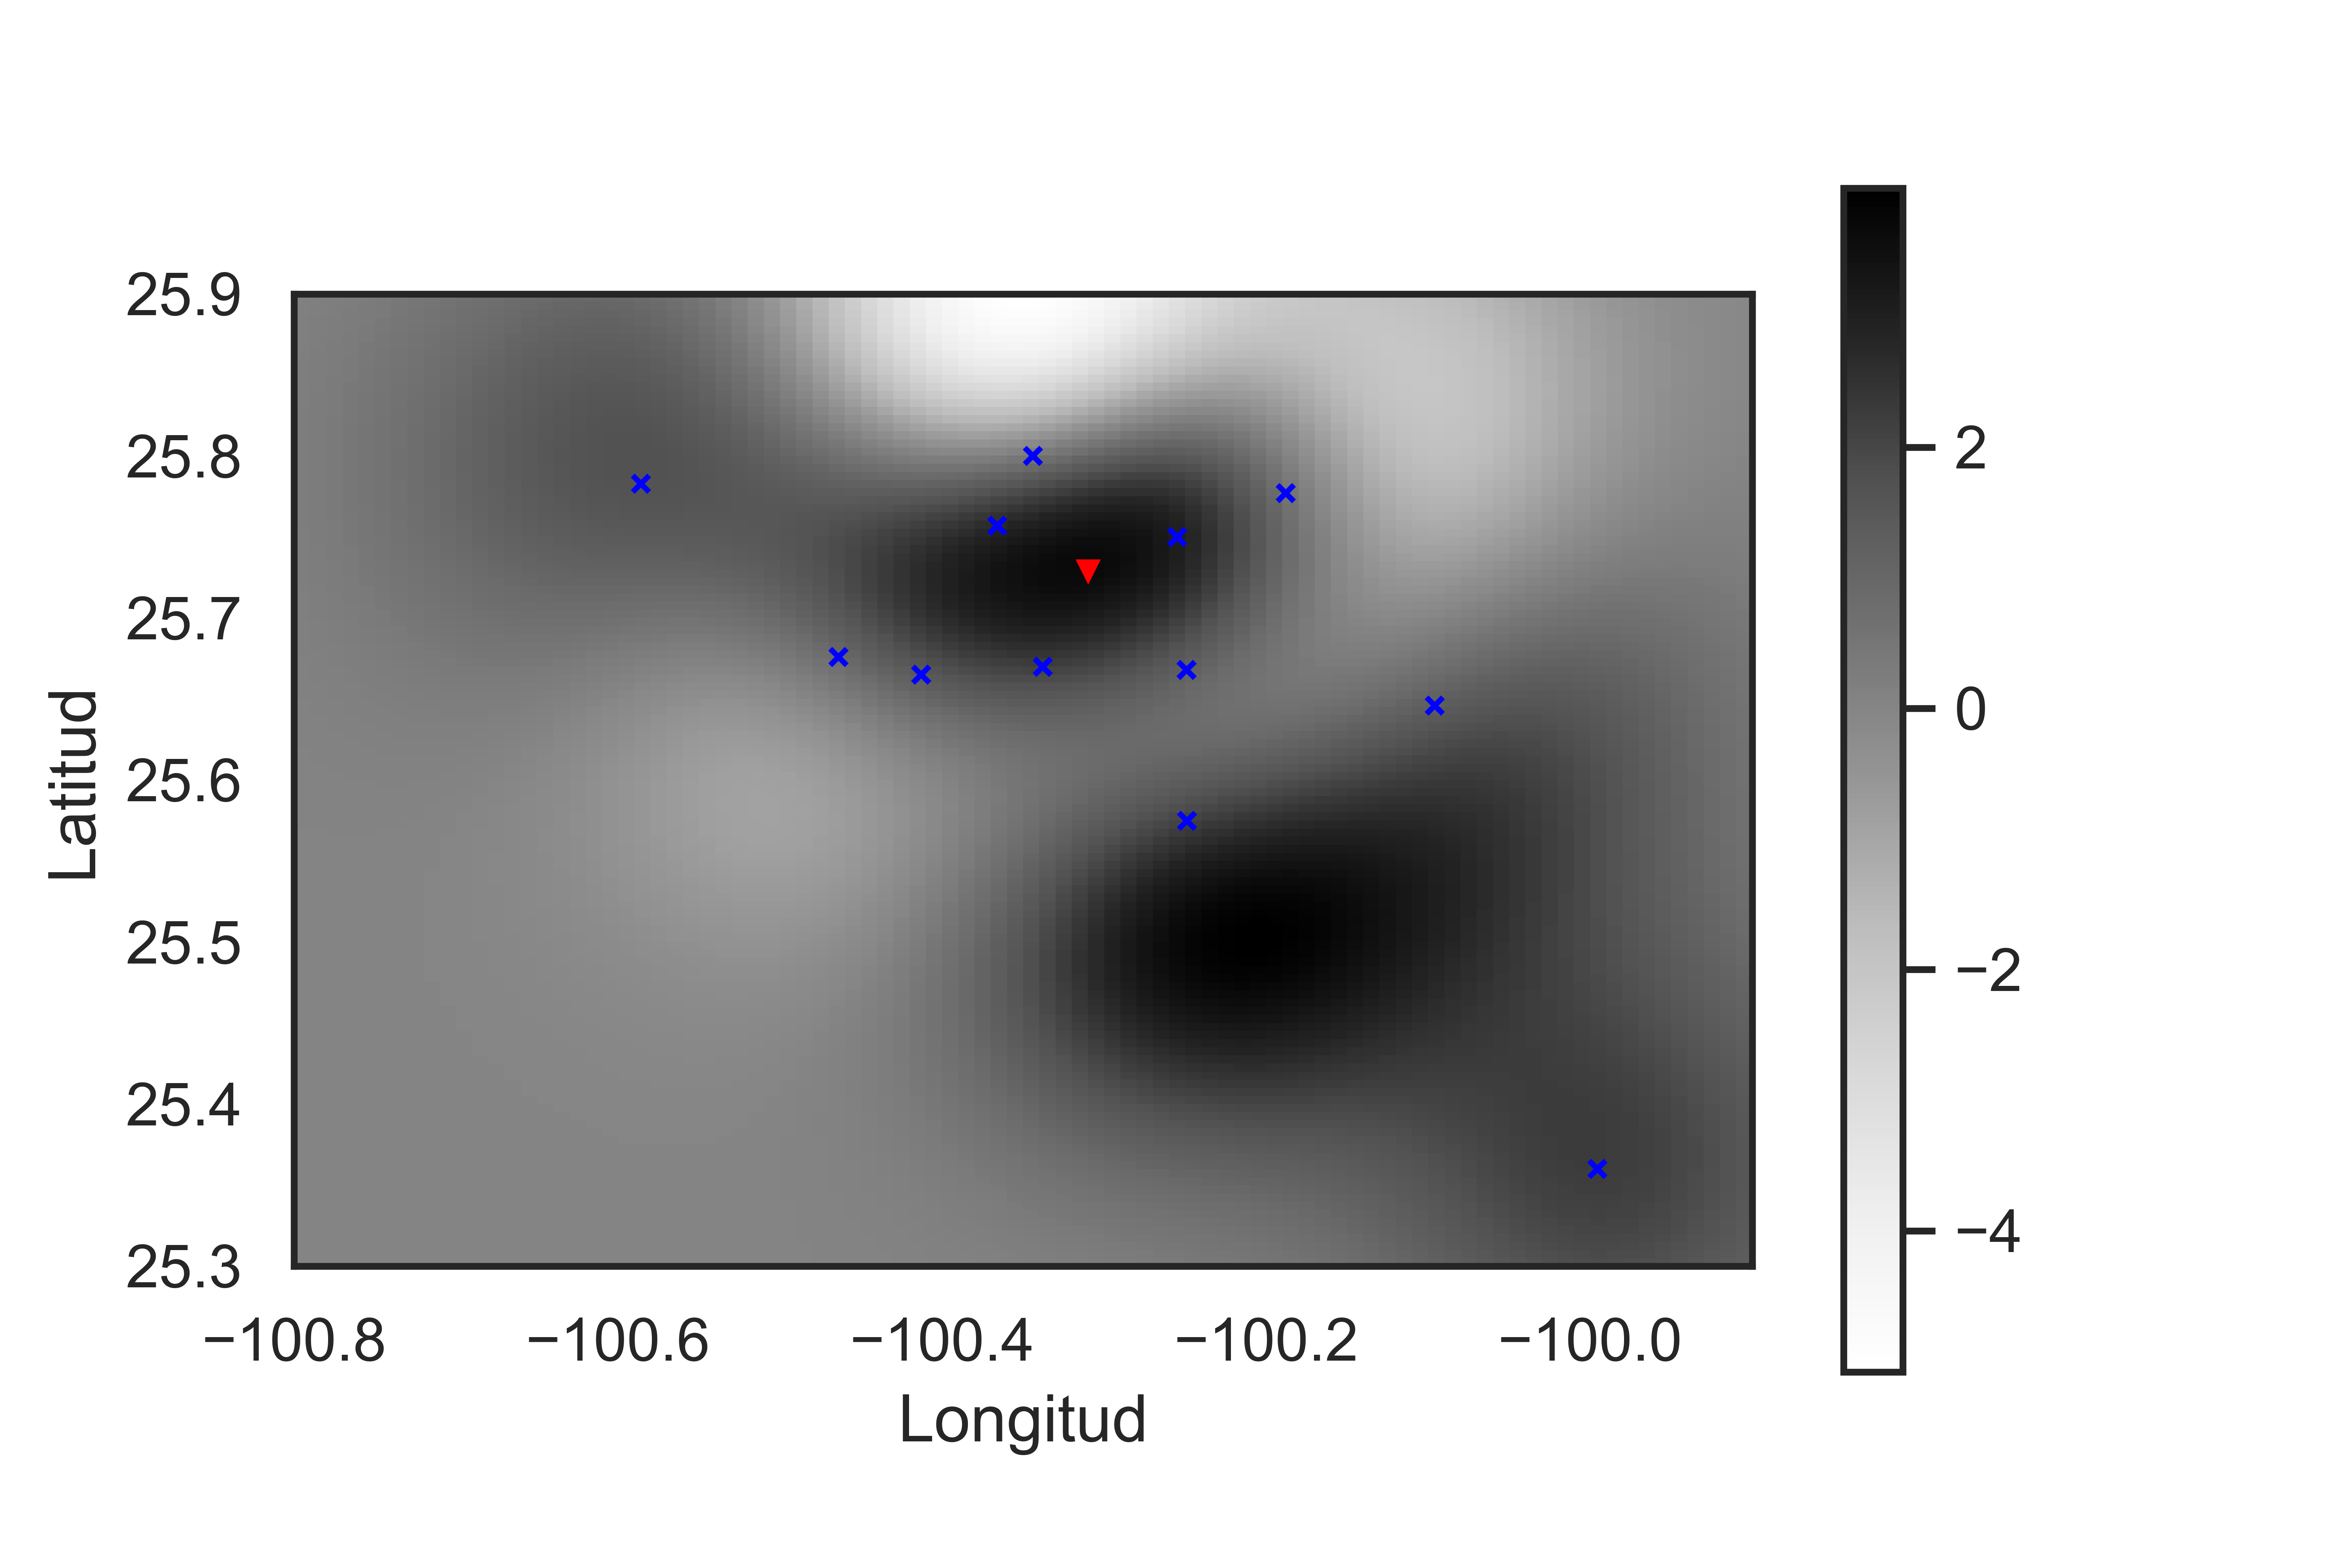
\includegraphics[width=4cm, height=4cm]{./brf_g_12_0_26302}}
\subfigure[FBR L] {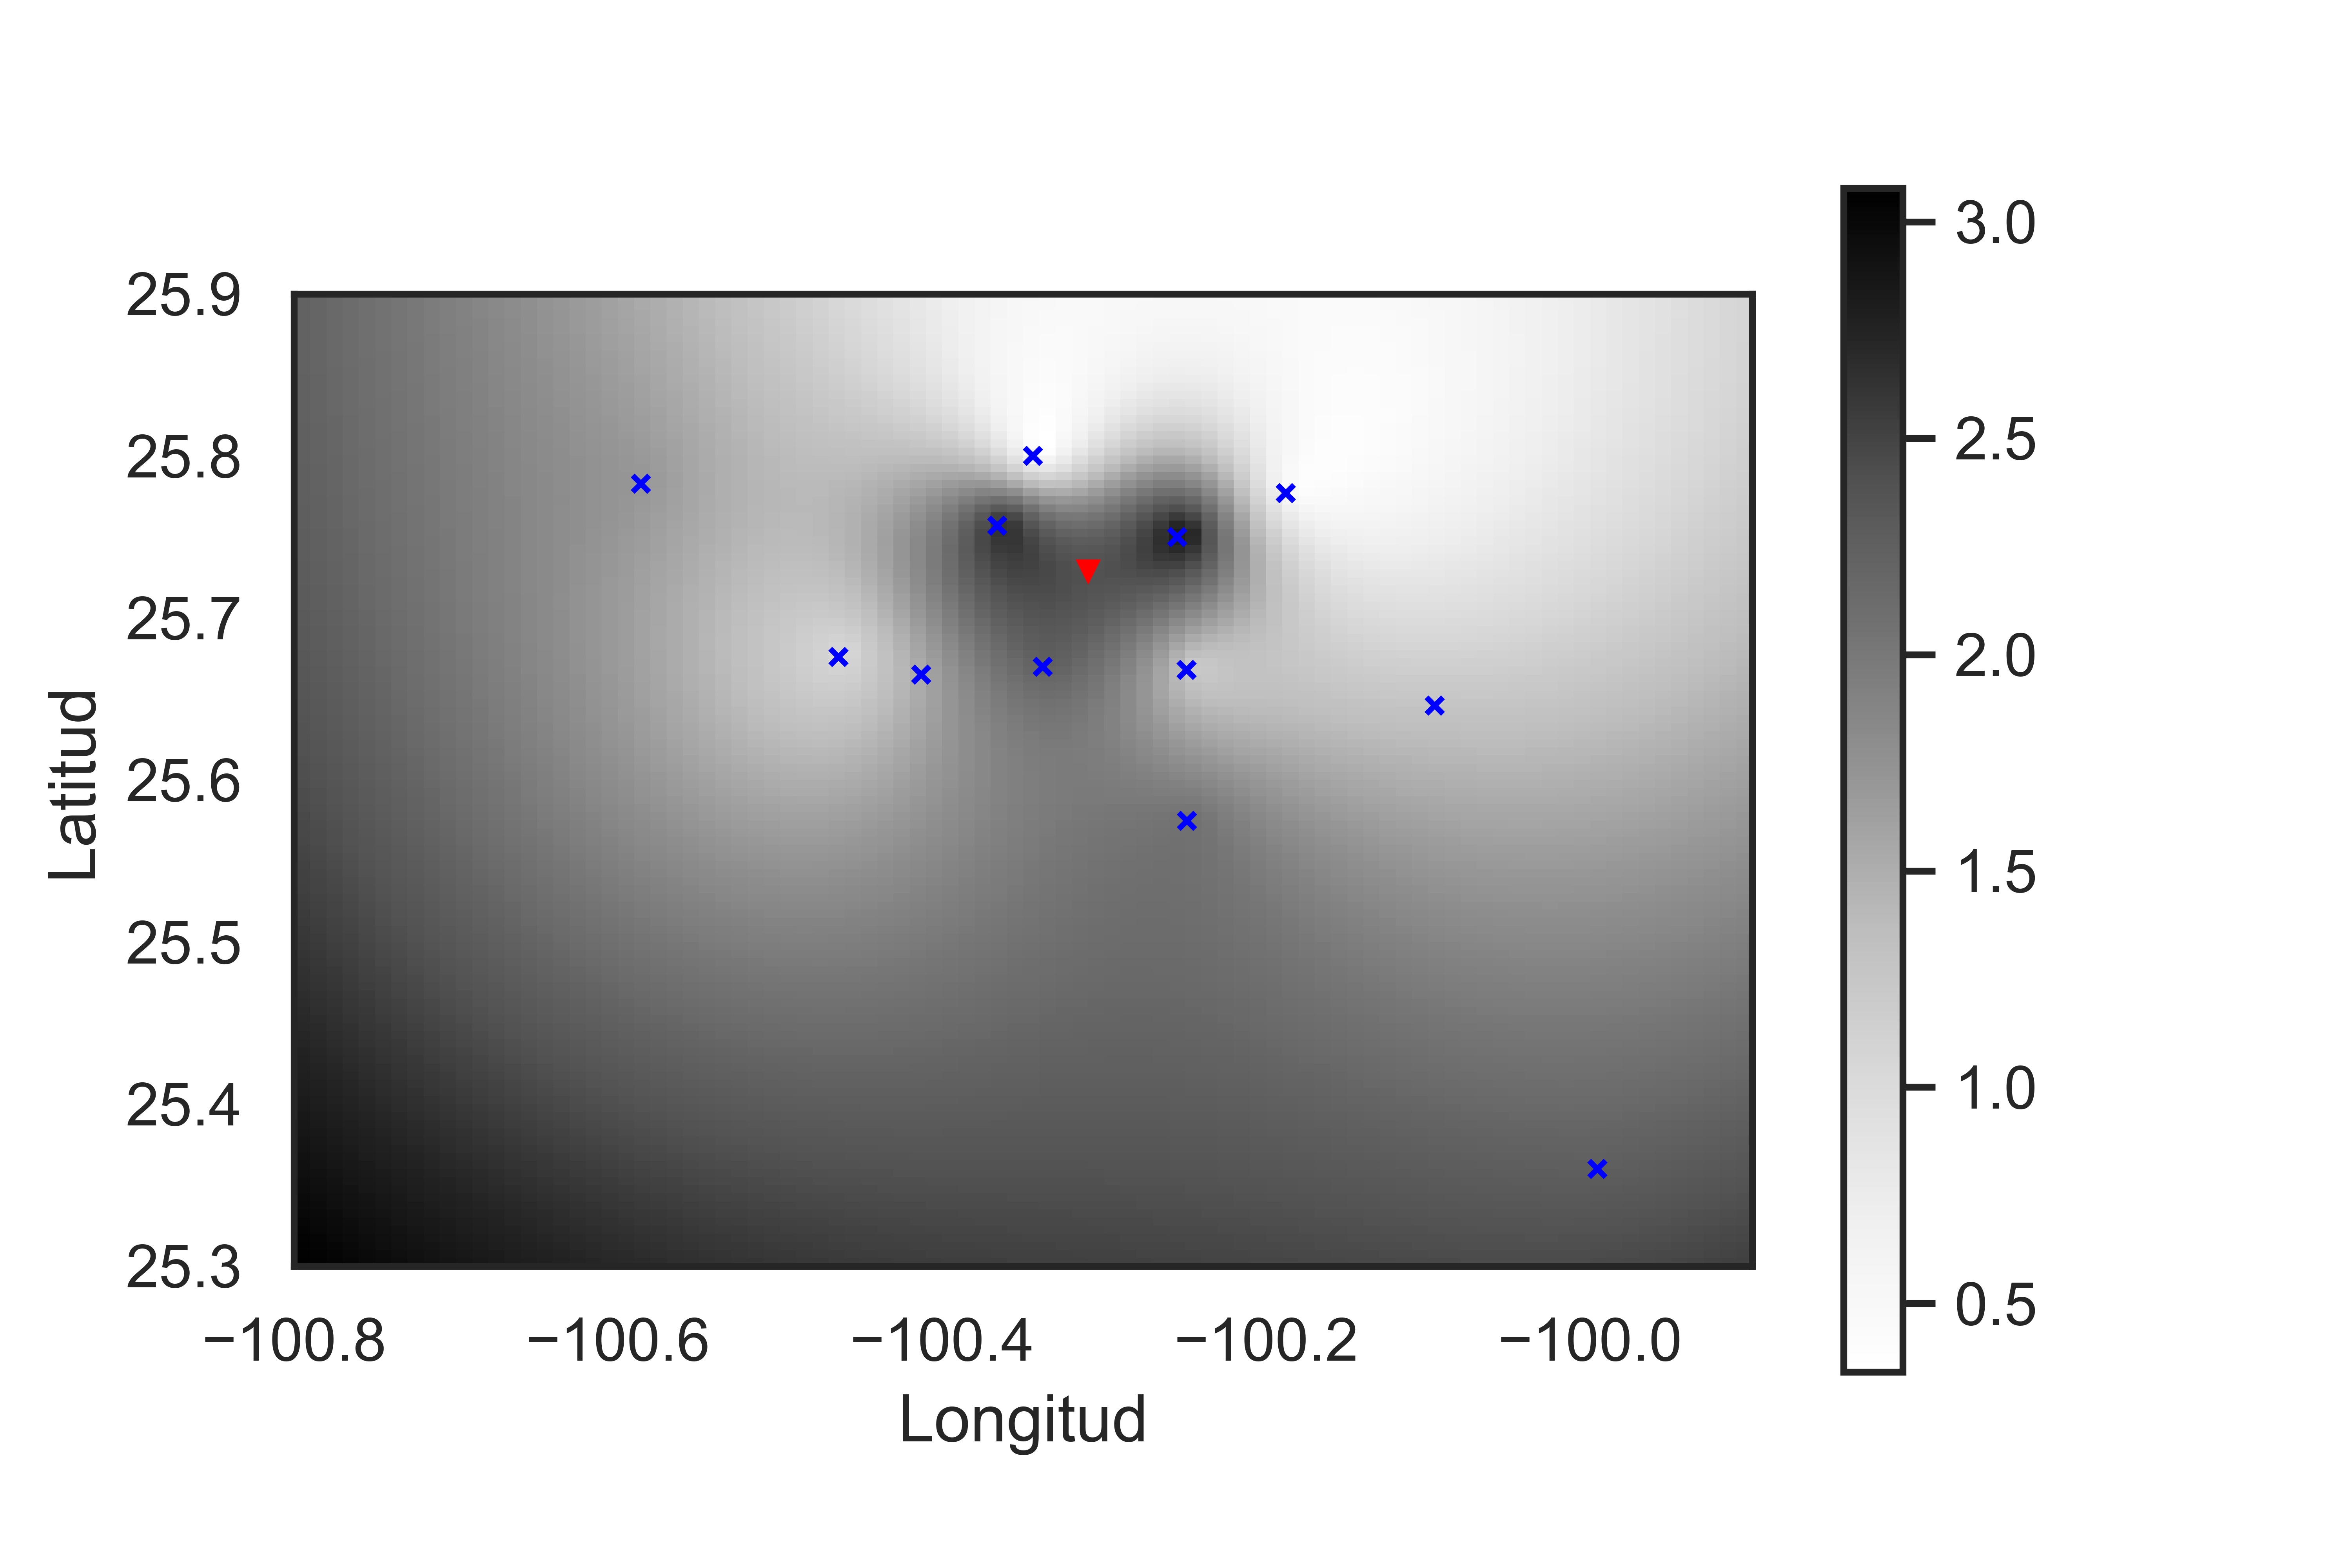
\includegraphics[width=4cm, height=4cm]{./brf_l_12_0_26302}}
\subfigure[FBR C] {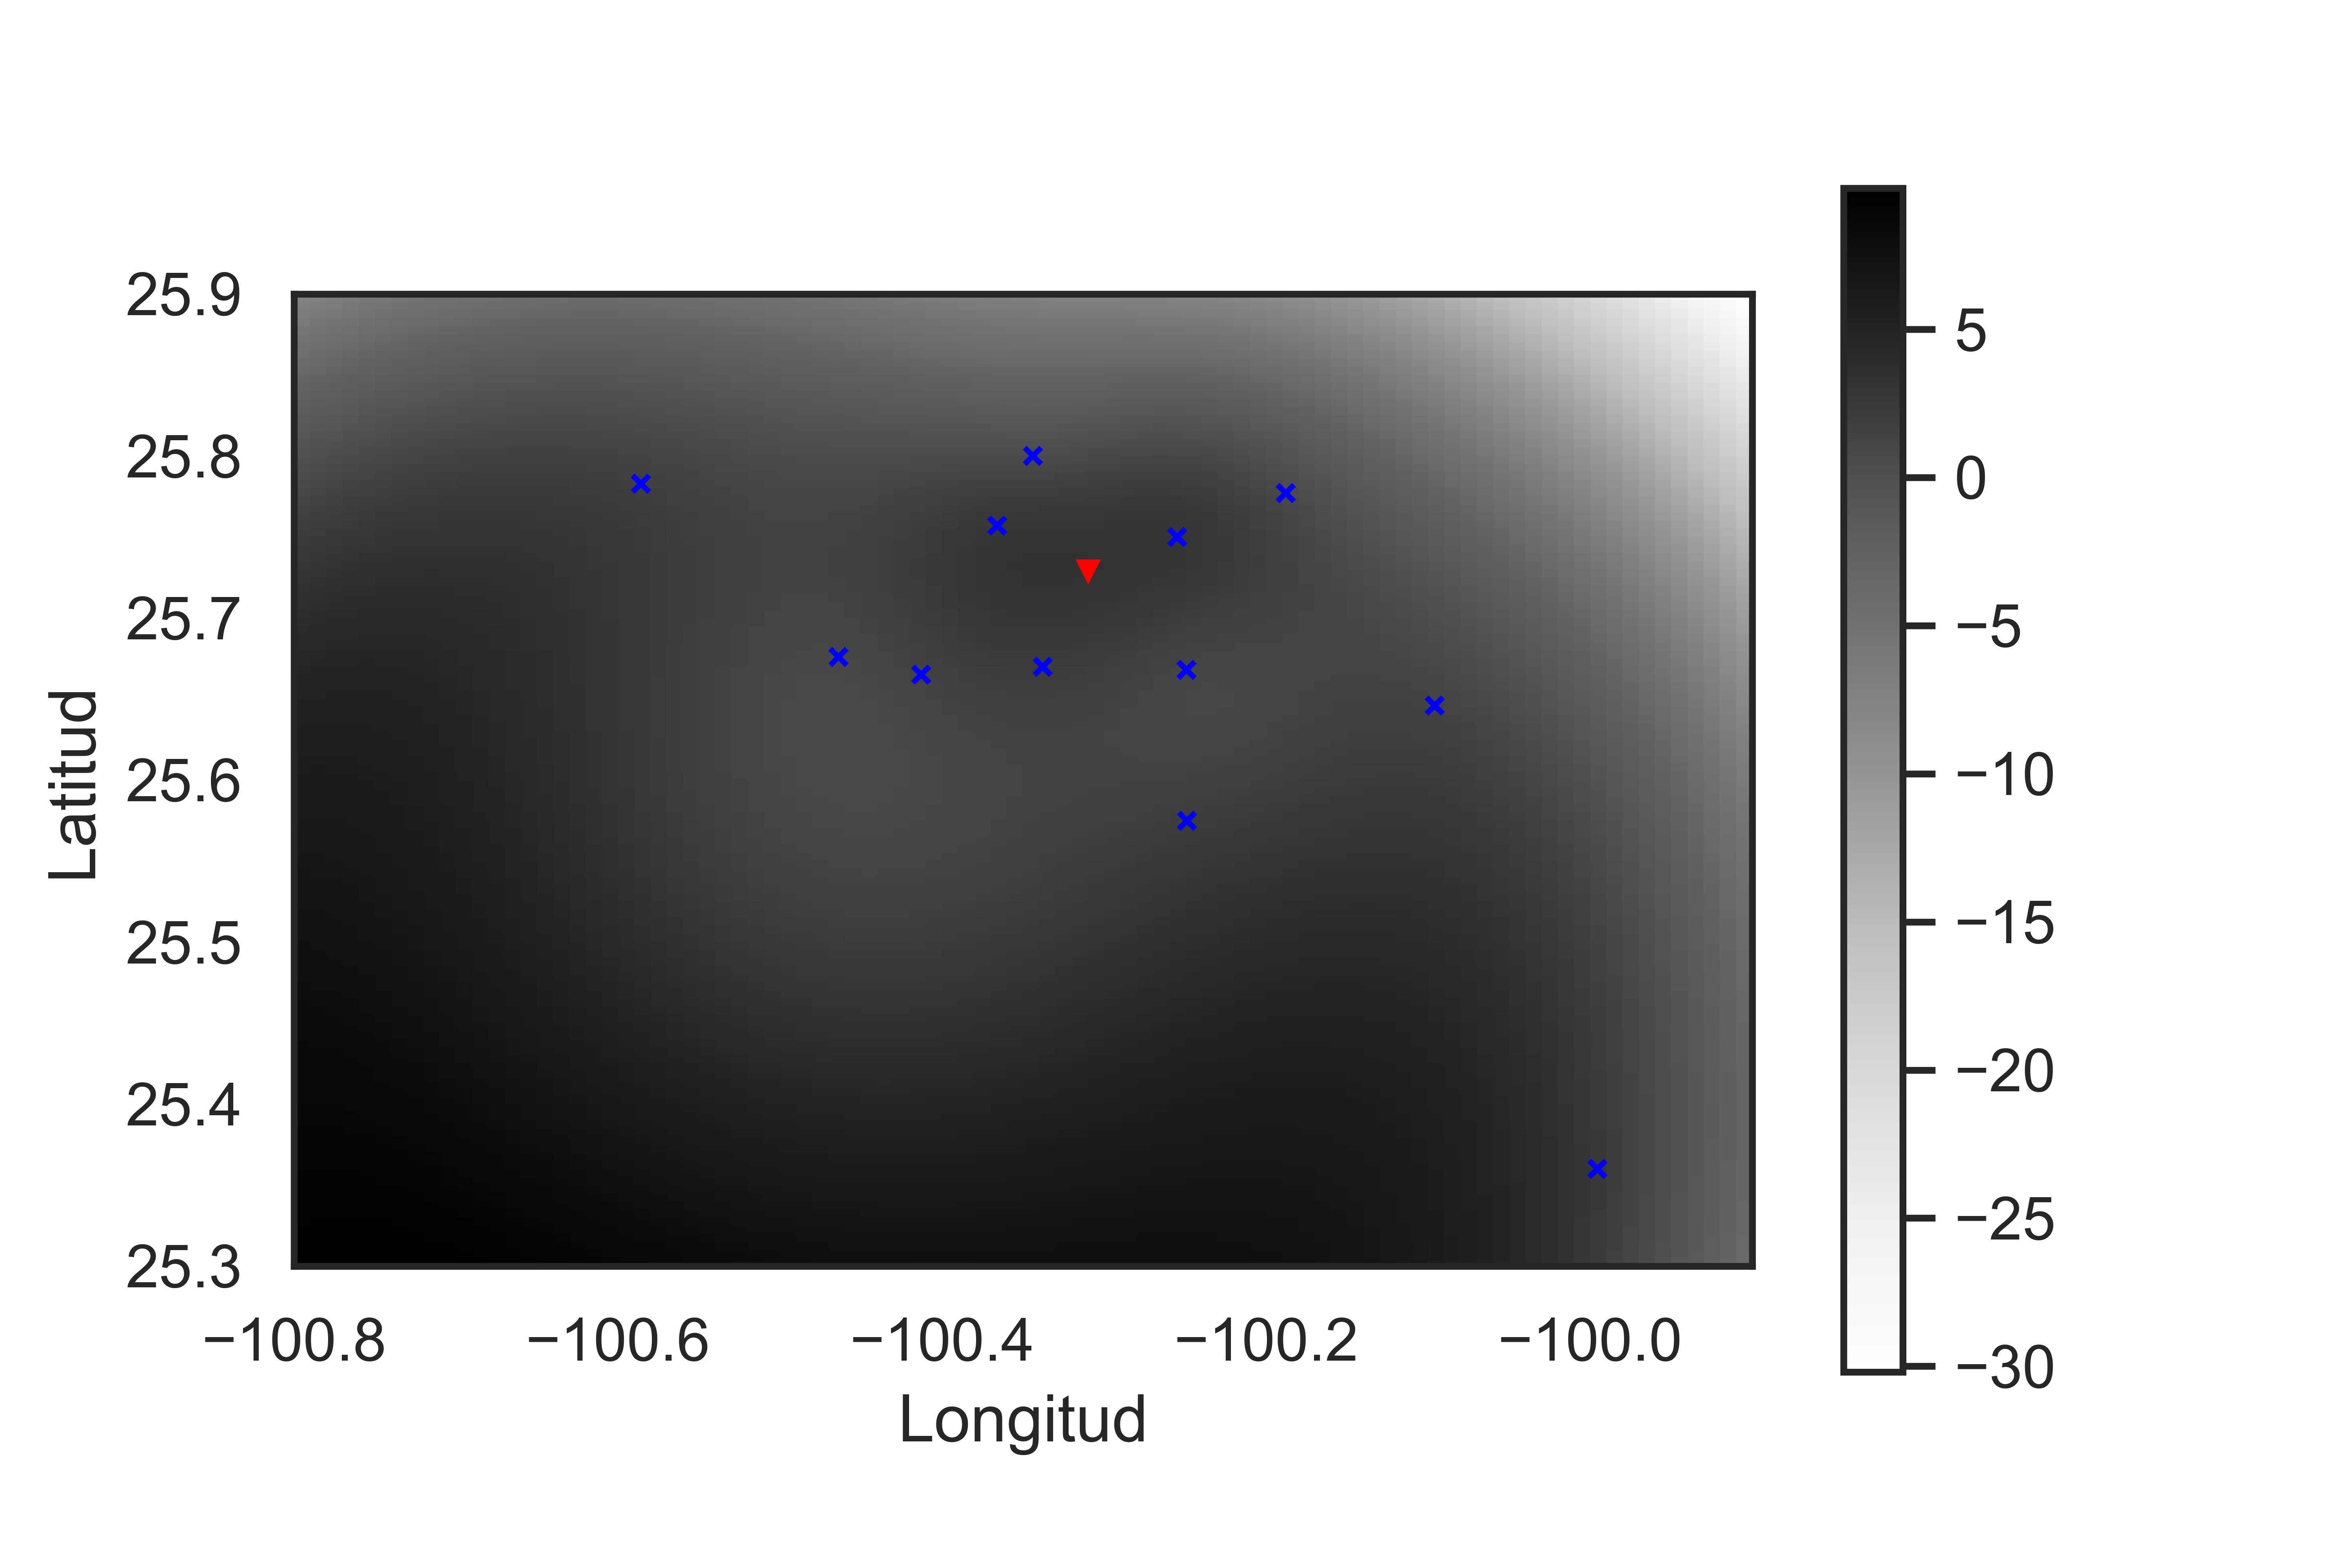
\includegraphics[width=4cm, height=4cm]{./brf_c_12_0_26302}}
\subfigure[FBR Q] {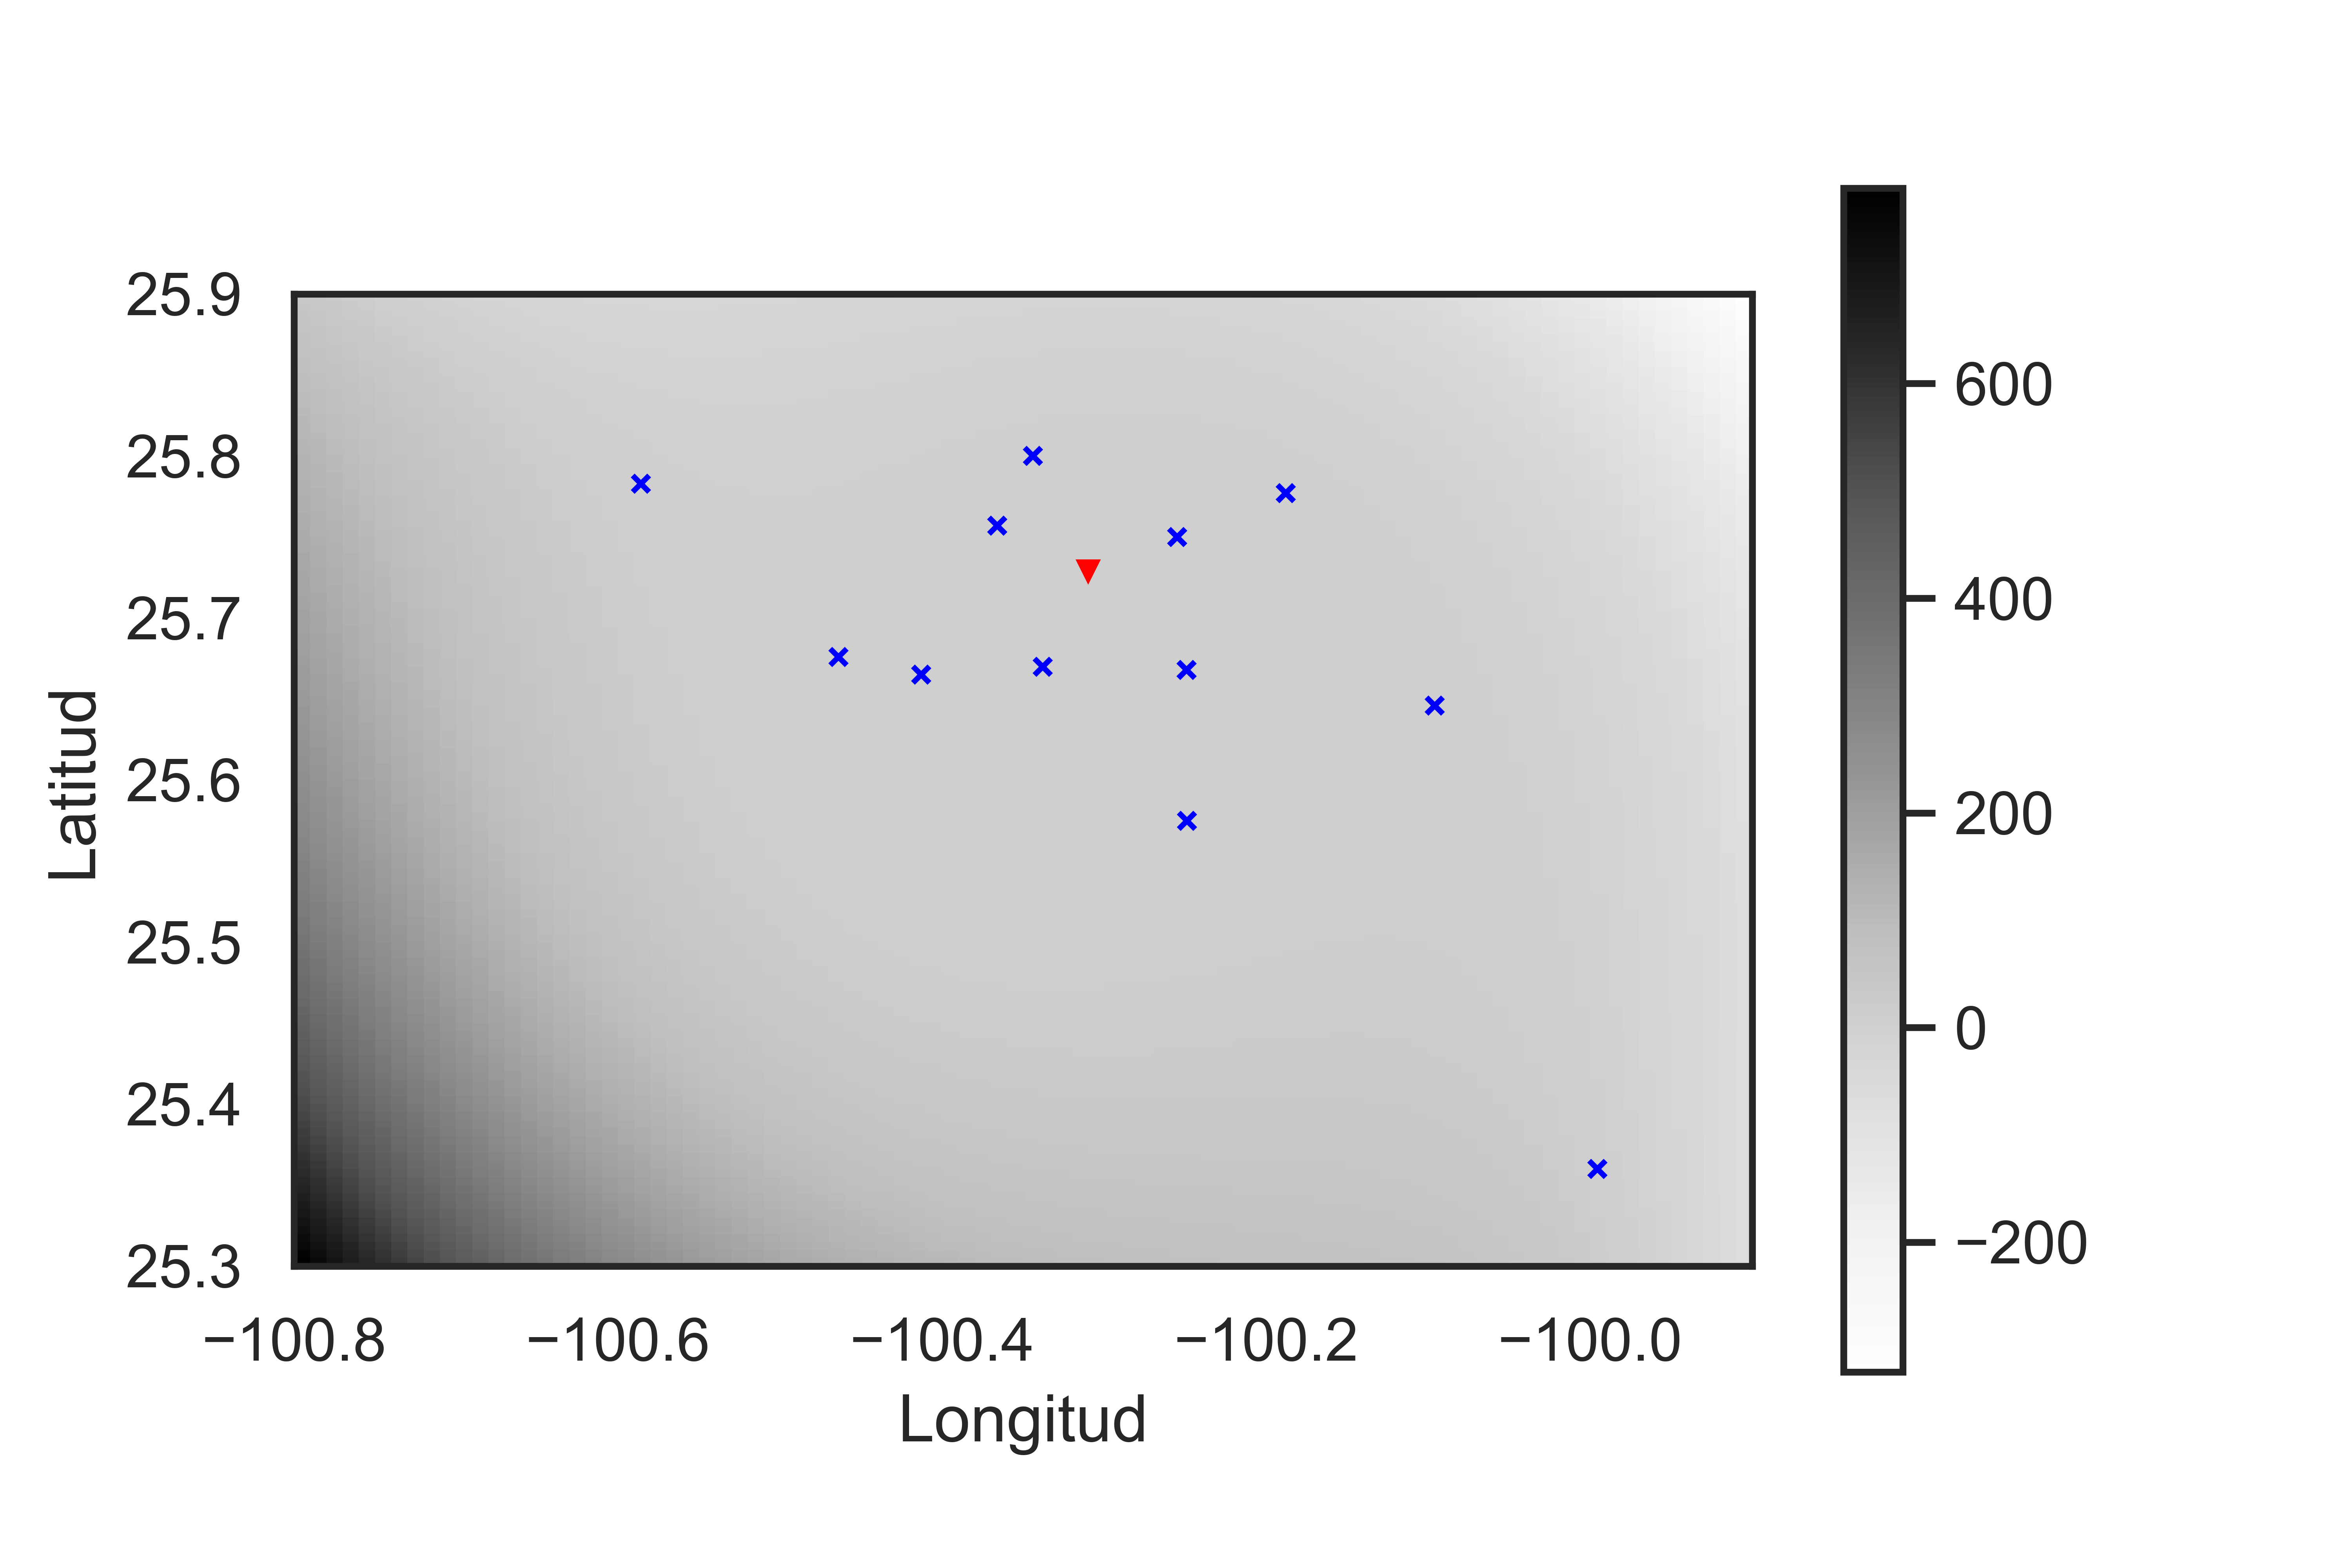
\includegraphics[width=4cm, height=4cm]{./brf_q_12_0_26302}}
\subfigure[FBR TPS] {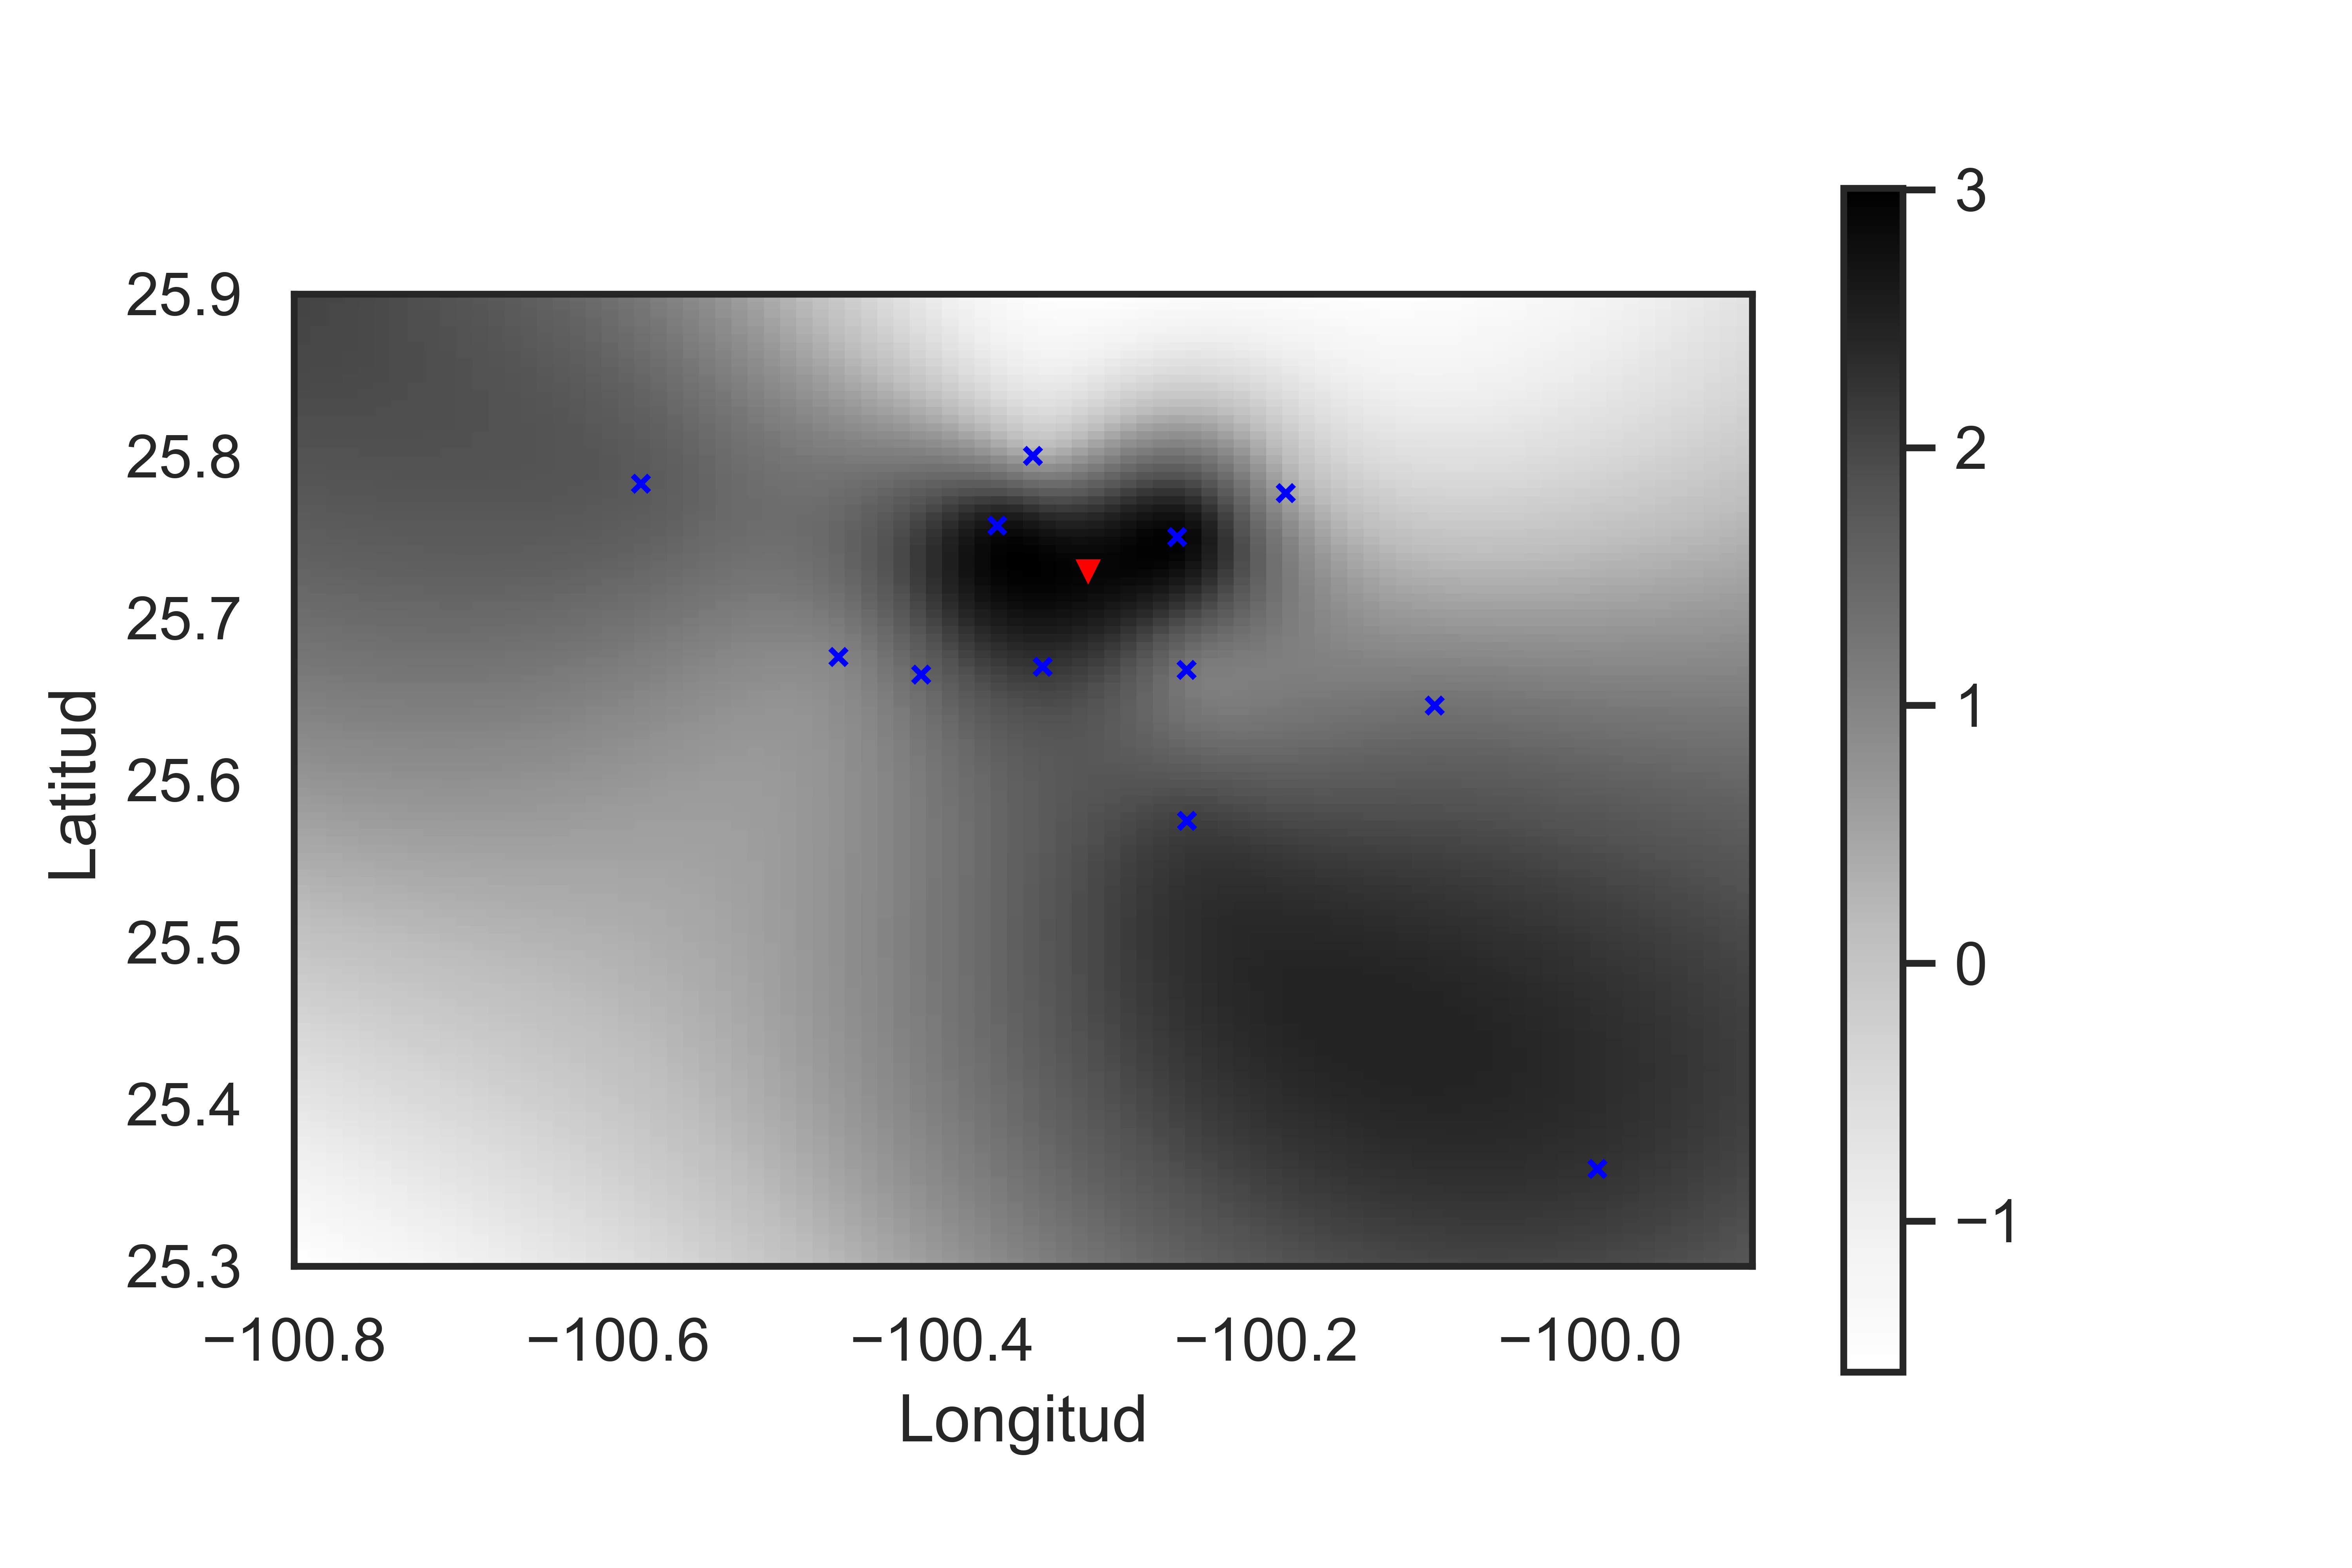
\includegraphics[width=4cm, height=4cm]{./brf_tps_12_0_26302}}
\subfigure[KO] {\includegraphics[width=4cm, height=4cm]{./ok_12_0_26302}}
\subfigure[KU] {\includegraphics[width=4cm, height=4cm]{./uk_12_0_26302}}
\caption{Interpolaciones de CO para 12 estaciones seleccionadas y 1 estación interpolada: Fecha (31-12-2018 23:00:00)}
\label{COfigure4}
\end{figure}






\subsection{Dióxido de Nitrógeno (NO$_{2}$)}

\begin{table}[H]
\centering
\caption{NO$_{2}$: 9 estaciones seleccionadas 4 estaciones interpoladas}
\begin{adjustbox}{max width=0.9\textwidth}
\begin{tabular}{|c|c|c|c|c|c|c|}
\hline
\multicolumn{7}{ |c| }{Métricas de error} \\ \hline
Método &MAPE &MAE &MAEP &RMSE &RMSEP &MSE \\ \hline
TV &0.79 &6.02 &0.57 &9.42 &0.90 &88.84\\
DIP &0.60 &4.49 &0.43 &7.59 &0.72 &57.64 \\
FBR M &$2.46\times10^{14}$ &$2.27\times10^{14}$ &$218\times10^{14}$ &$1.44\times10^{17}$ &$1.39\times10^{16}$ &$2.10\times10^{34}$ \\
FBR IM &0.81 &6.73 &0.64 &10.03 &0.96 &100.72 \\
FBR G &$6.26\times10^{13}$ &$2.62\times10^{14}$ &$2.52\times10^{13}$ &$4.92\times10^{16}$ &$4.72\times10^{15}$ &$2.42\times10^{33}$ \\
FBR L &2.13 &13.29 &1.27 &54.76 &5.25 &2,999.60 \\
FBR C &$1.20\times10^{17}$ &$6.57\times10^{17}$ &$6.31\times10^{16}$ &$2.46\times10^{18}$ &$2.36\times10^{17}$ &$6.06\times10^{36}$ \\
FBR Q &$2.78\times10^{17}$ &$1.64\times10^{18}$ &$1.57\times10^{17}$ &$3.88\times10^{18}$ &$3.72\times10^{17}$ &$1.50\times10^{37}$ \\
FBR TPS &1.95 &12.46 &1.19 &98.09 &9.41 &9,621.95 \\
KO &0.63 &4.66 &0.44 &7.87 &0.75 &61.98 \\
KU &0.83 &6.26 &0.60 &14.13 &1.35 &199.79 \\\hline
\end{tabular}
\end{adjustbox}
\label{tabNO2}
\end{table}

De la tabla \ref{tabNO2}, en la cual se utilizan nueve estaciones para interpolar cuatro más, podemos ver que los métodos que obtiene peores resultados de predicción son los métodos de Funciones de Base Radial, a excepción de los métodos inverso multicuadrático, lineal y {\em thin plate splines} (FBR I,  FBR L y FBR TPS), entre los métodos deterministas, DIP obtuvo el menor MAPE, MAE, MAEP, RMSE, RMSEP y MSE; mientras que de los métodos geoestadísticos el método KO obtuvo el menor MAPE, MAE, MAEP, RMSE, RMSEP y MSE. En general, DIP y KO son mejores que el resto de los métodos pero DIP es mejor que KO ya que en los errores MAPE, MAE, MAEP, RMSE, RMSEP y MSE encontró mejores resultados que los errores de KO. En la figura \ref{NO2figure1}, se pueden observar las interpolaciones de cada método, donde las puntos azules son las estaciones seleccionadas y los puntos rojos son las estaciones interpoladas.


\begin{figure}[H]
\centering
\subfigure[TV] {\includegraphics[width=4cm, height=4cm]{./voronoi_9_2_26302}}
\subfigure[DIP] {\includegraphics[width=4cm, height=4cm]{./idw_9_2_26302}}
\subfigure[FBR M] {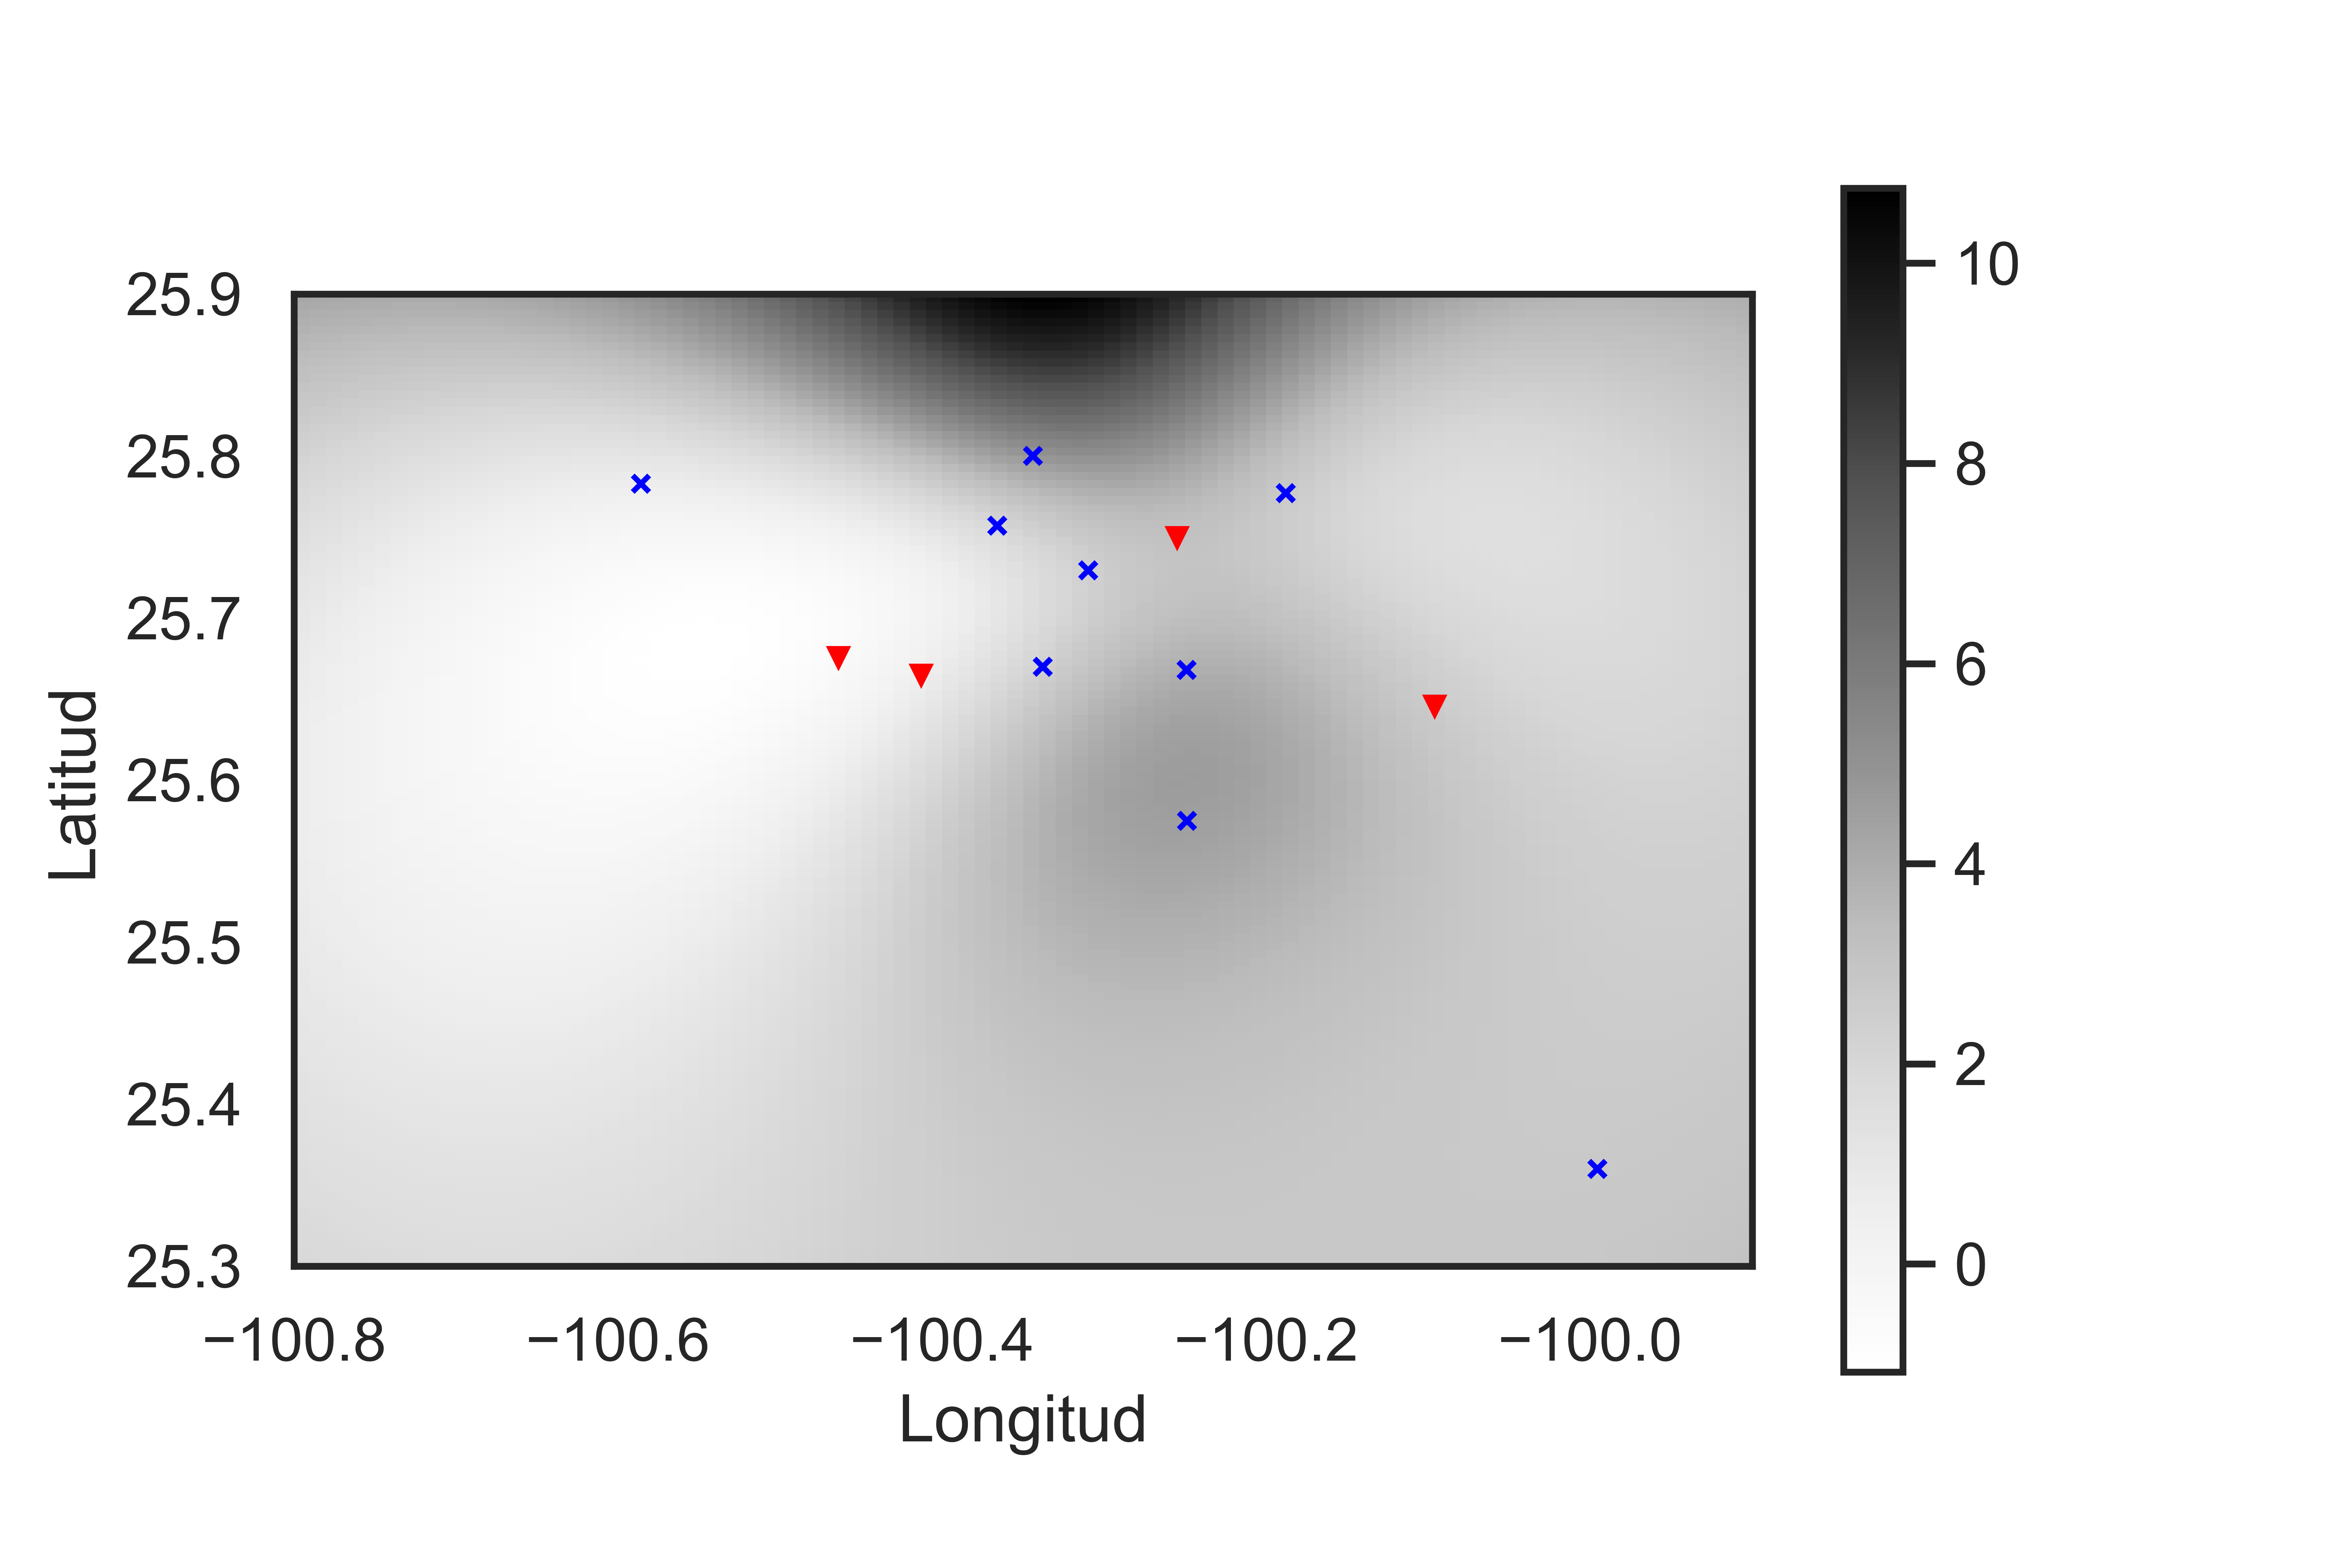
\includegraphics[width=4cm, height=4cm]{./brf_m_9_2_26302}}
\subfigure[FBR I] {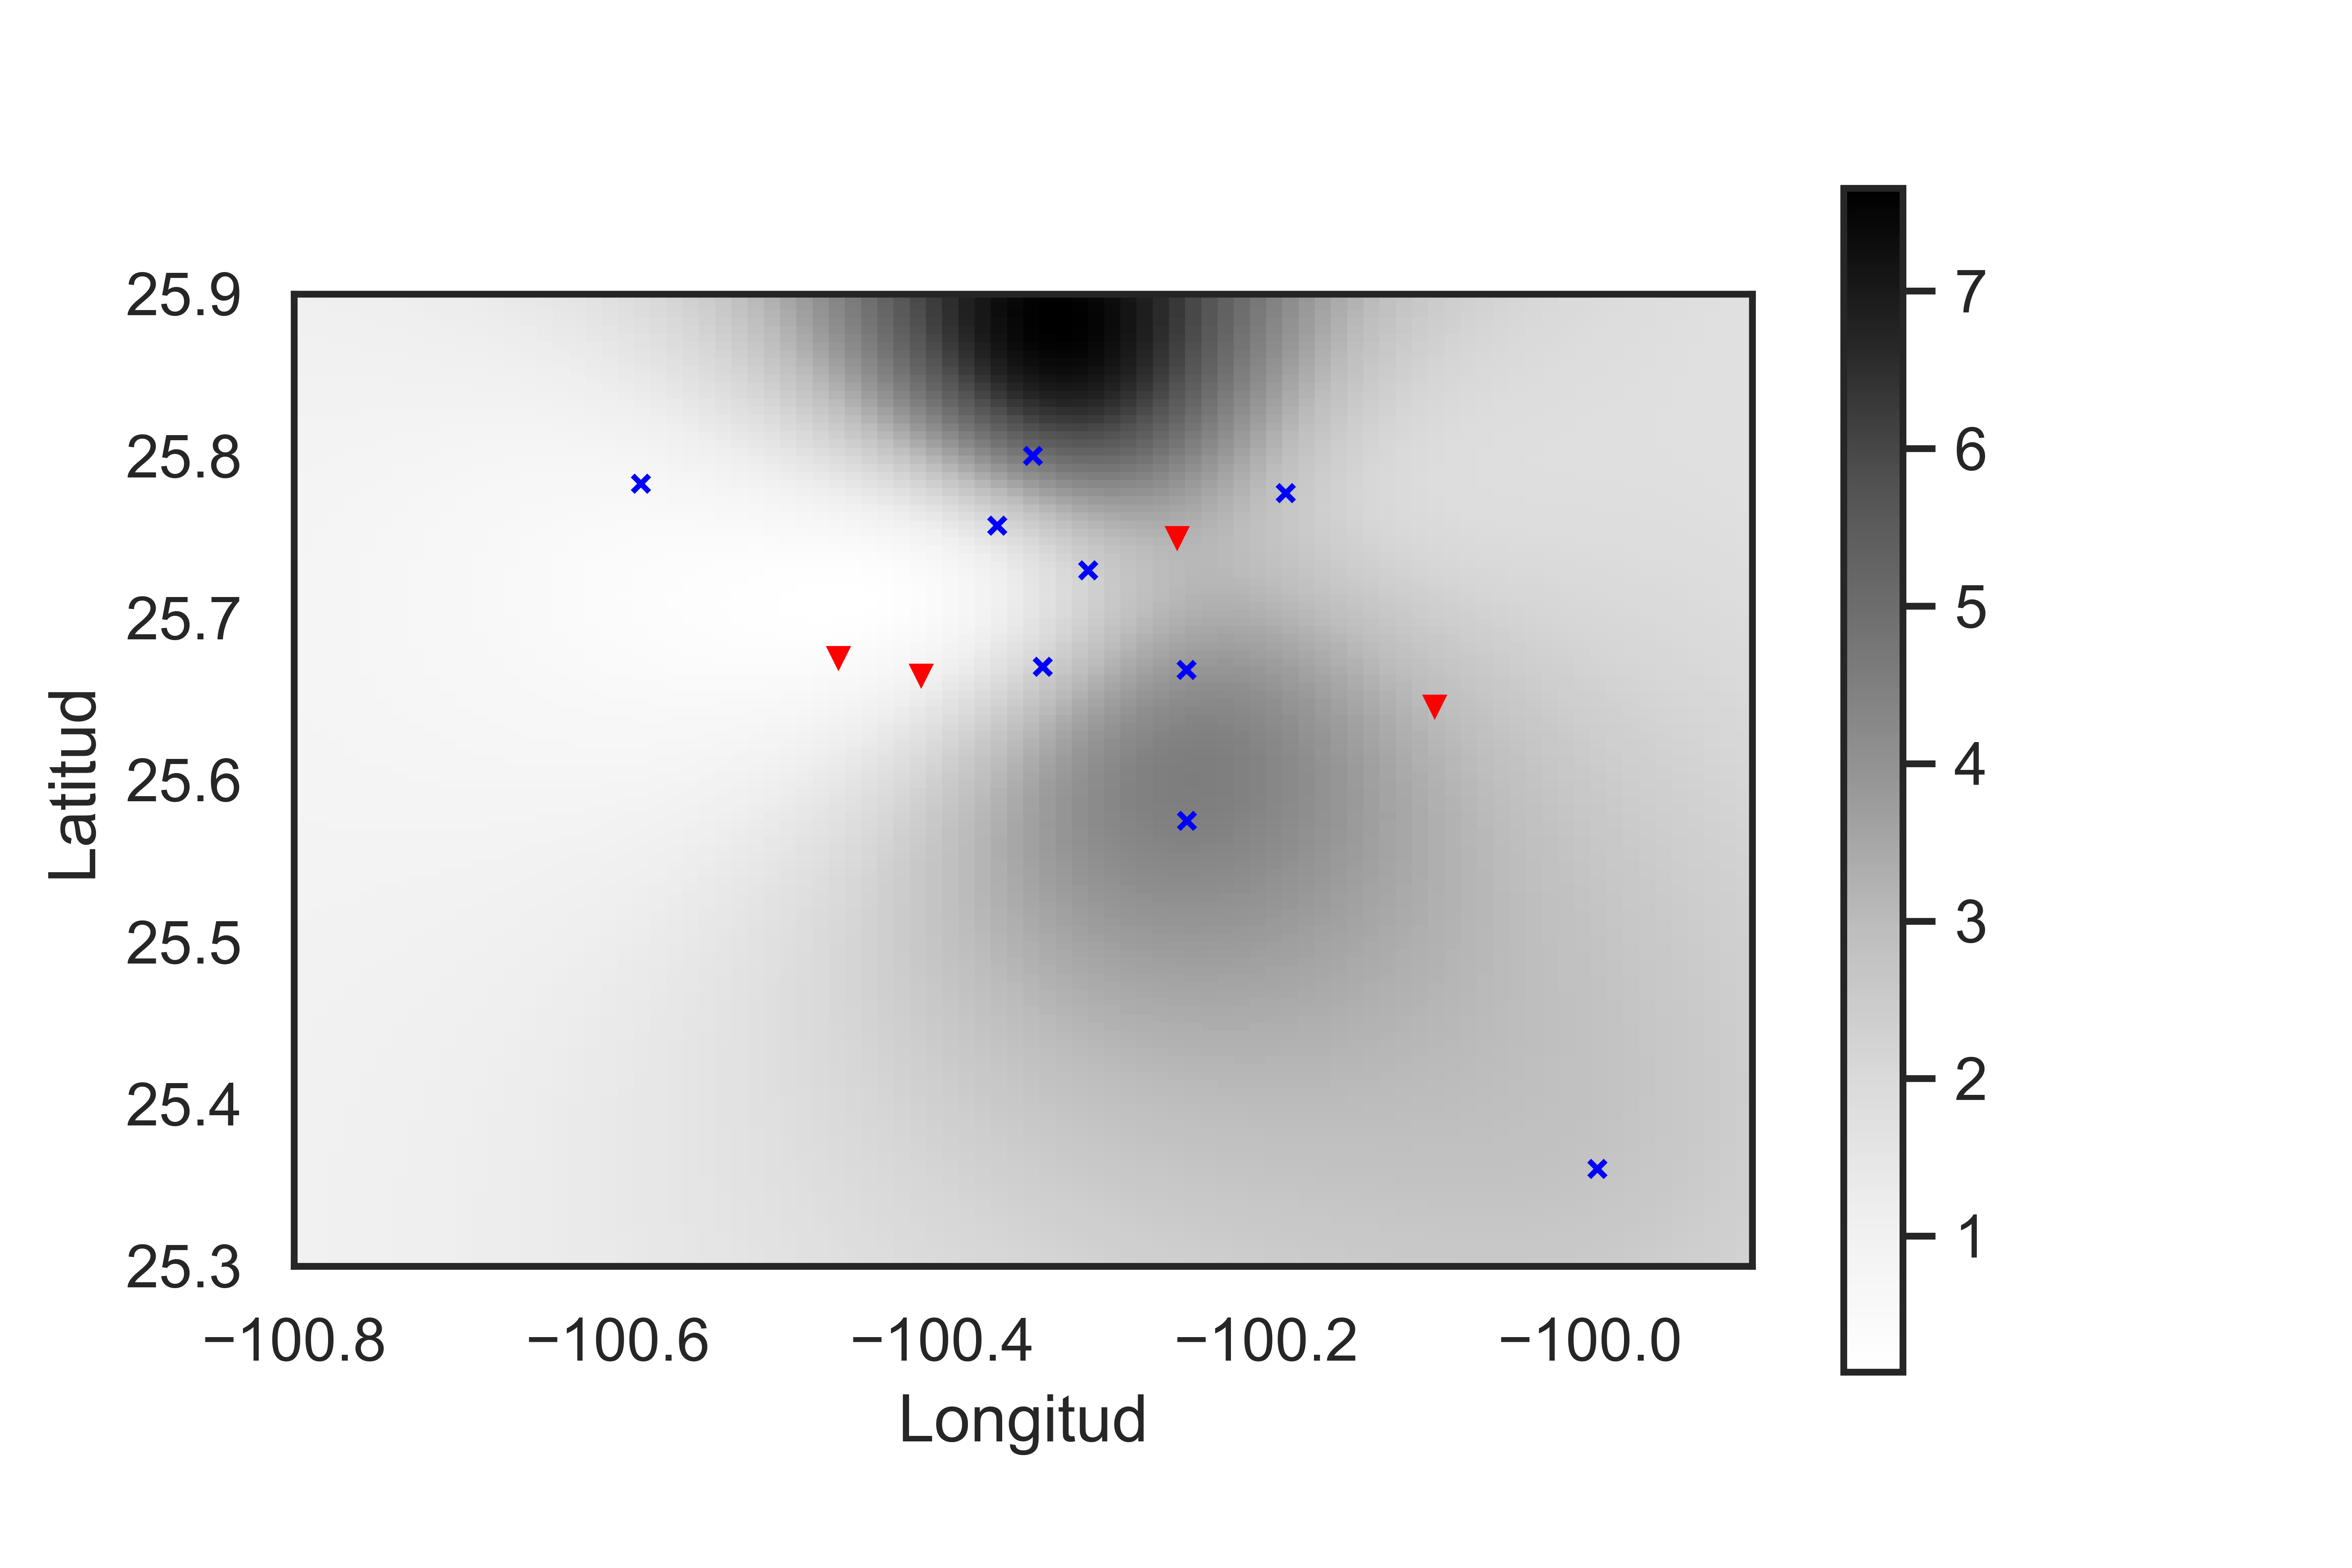
\includegraphics[width=4cm, height=4cm]{./brf_i_9_2_26302}}
\subfigure[FBR G] {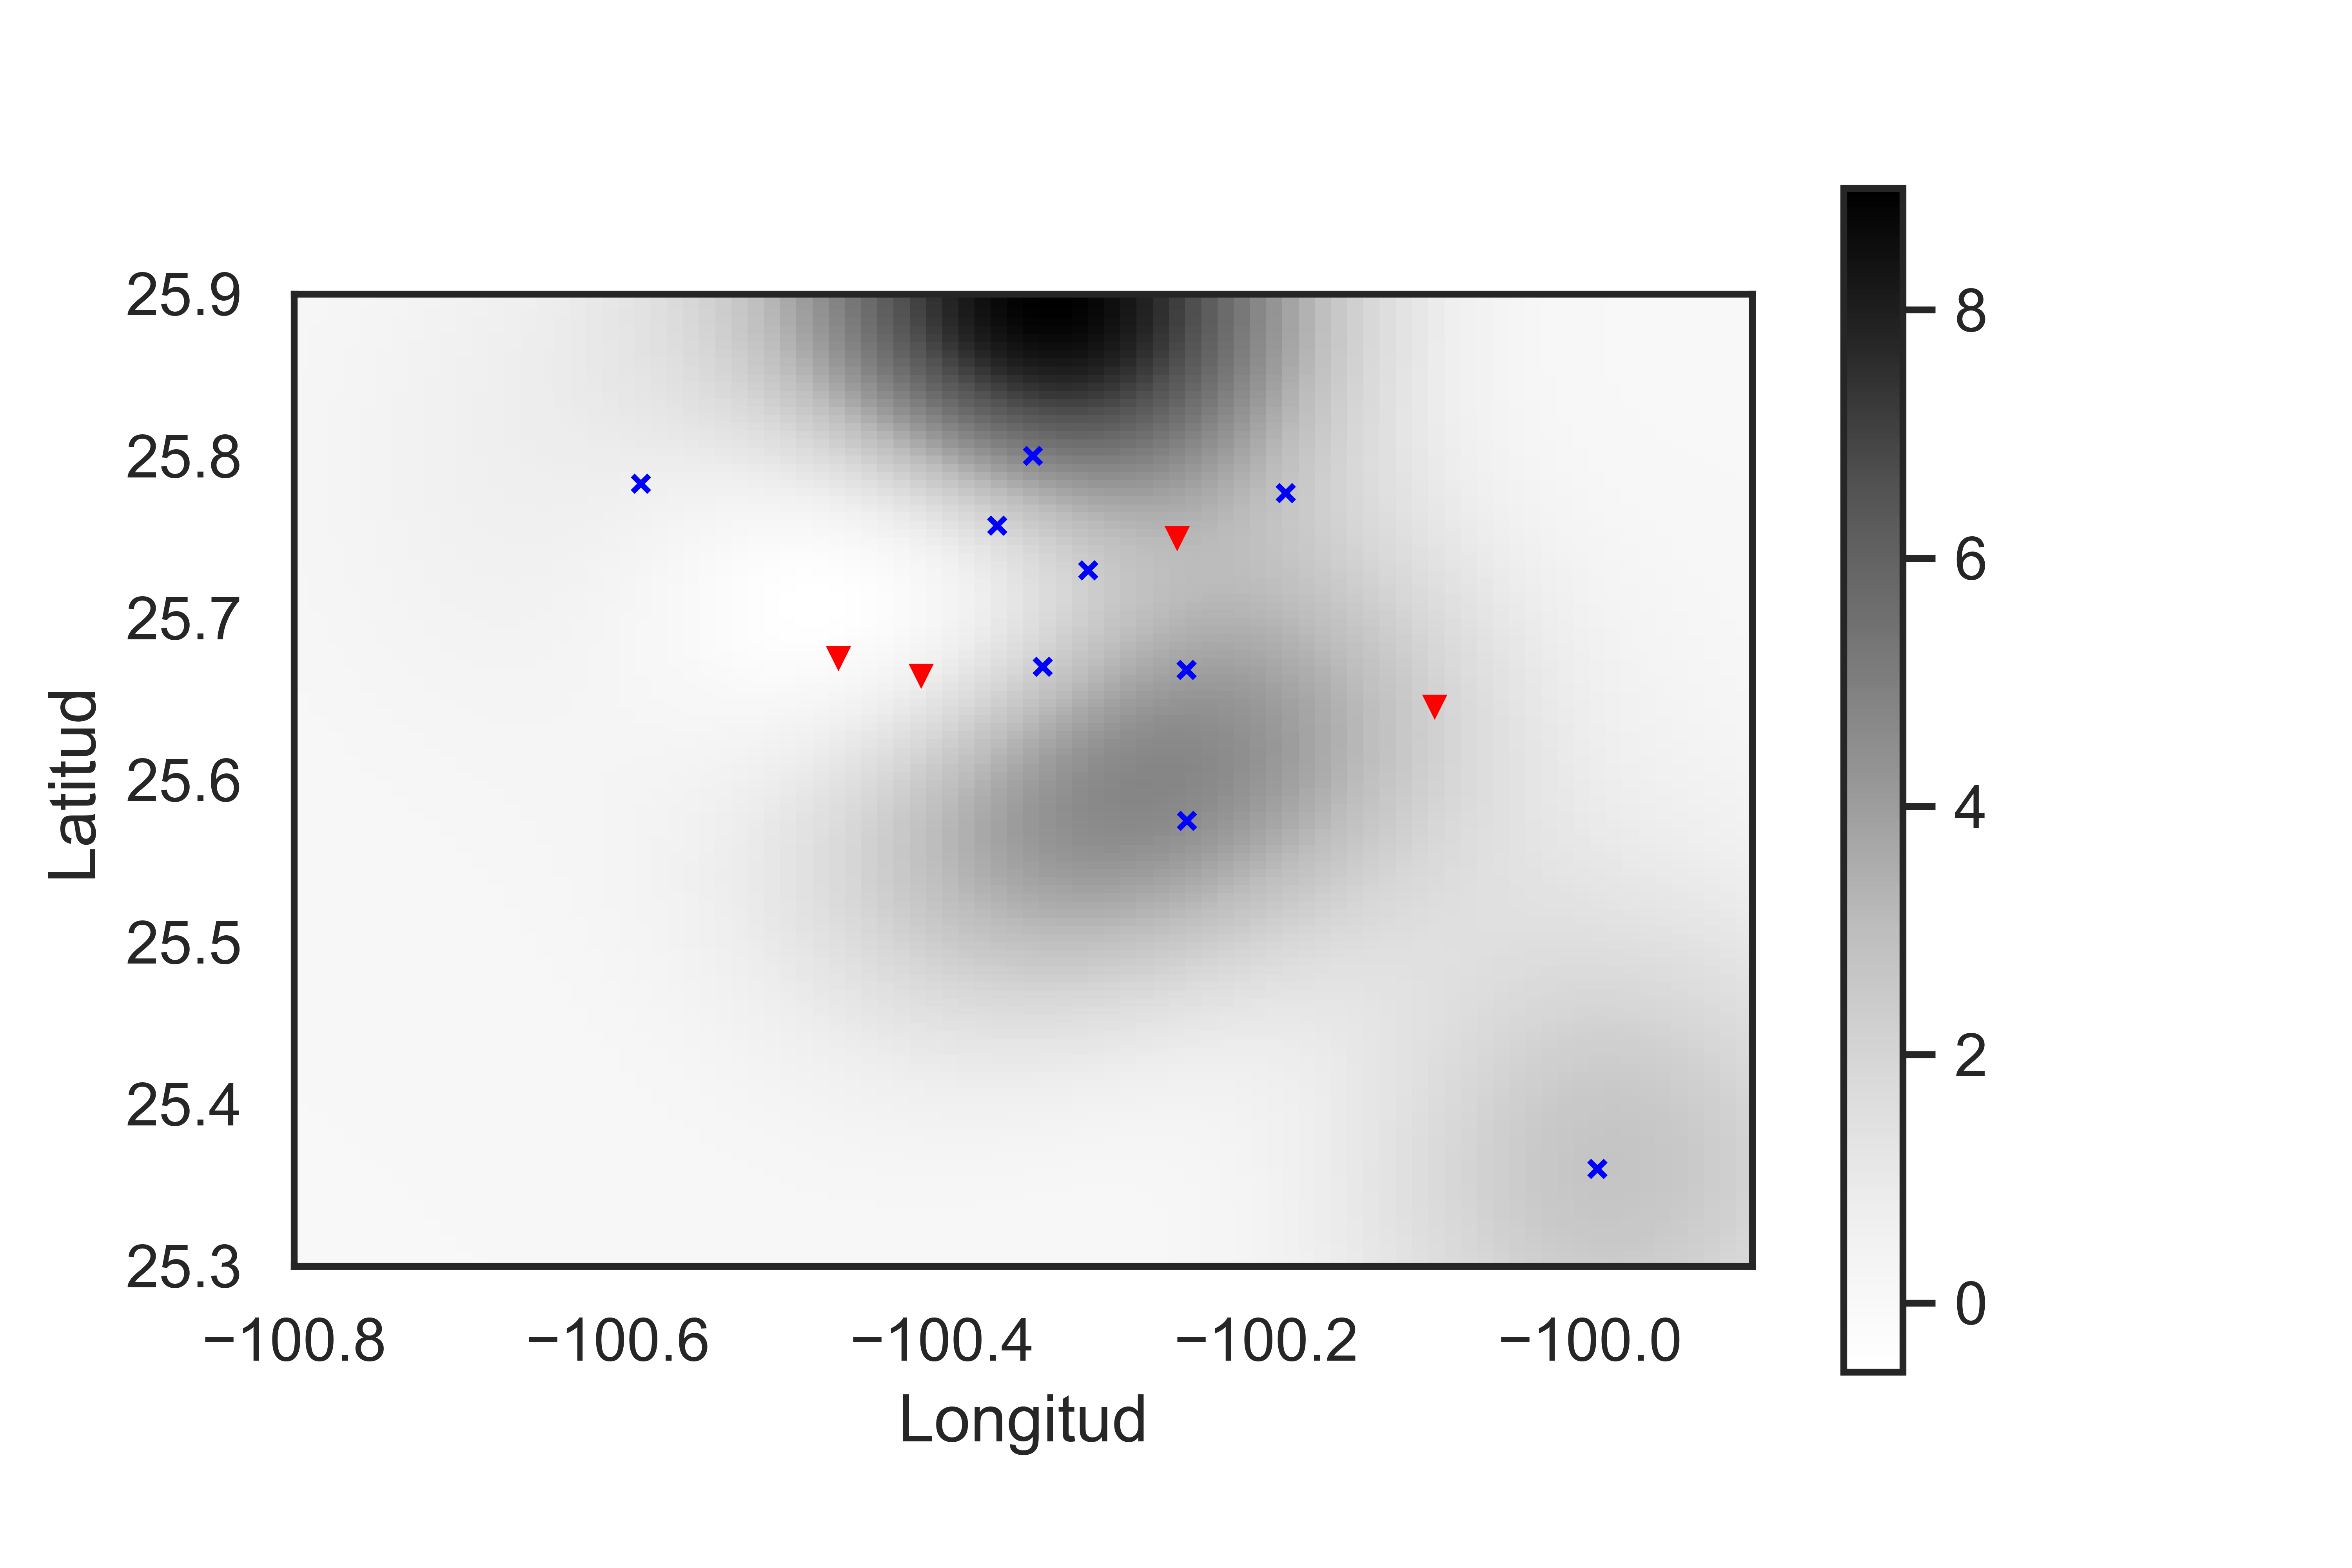
\includegraphics[width=4cm, height=4cm]{./brf_g_9_2_26302}}
\subfigure[FBR L] {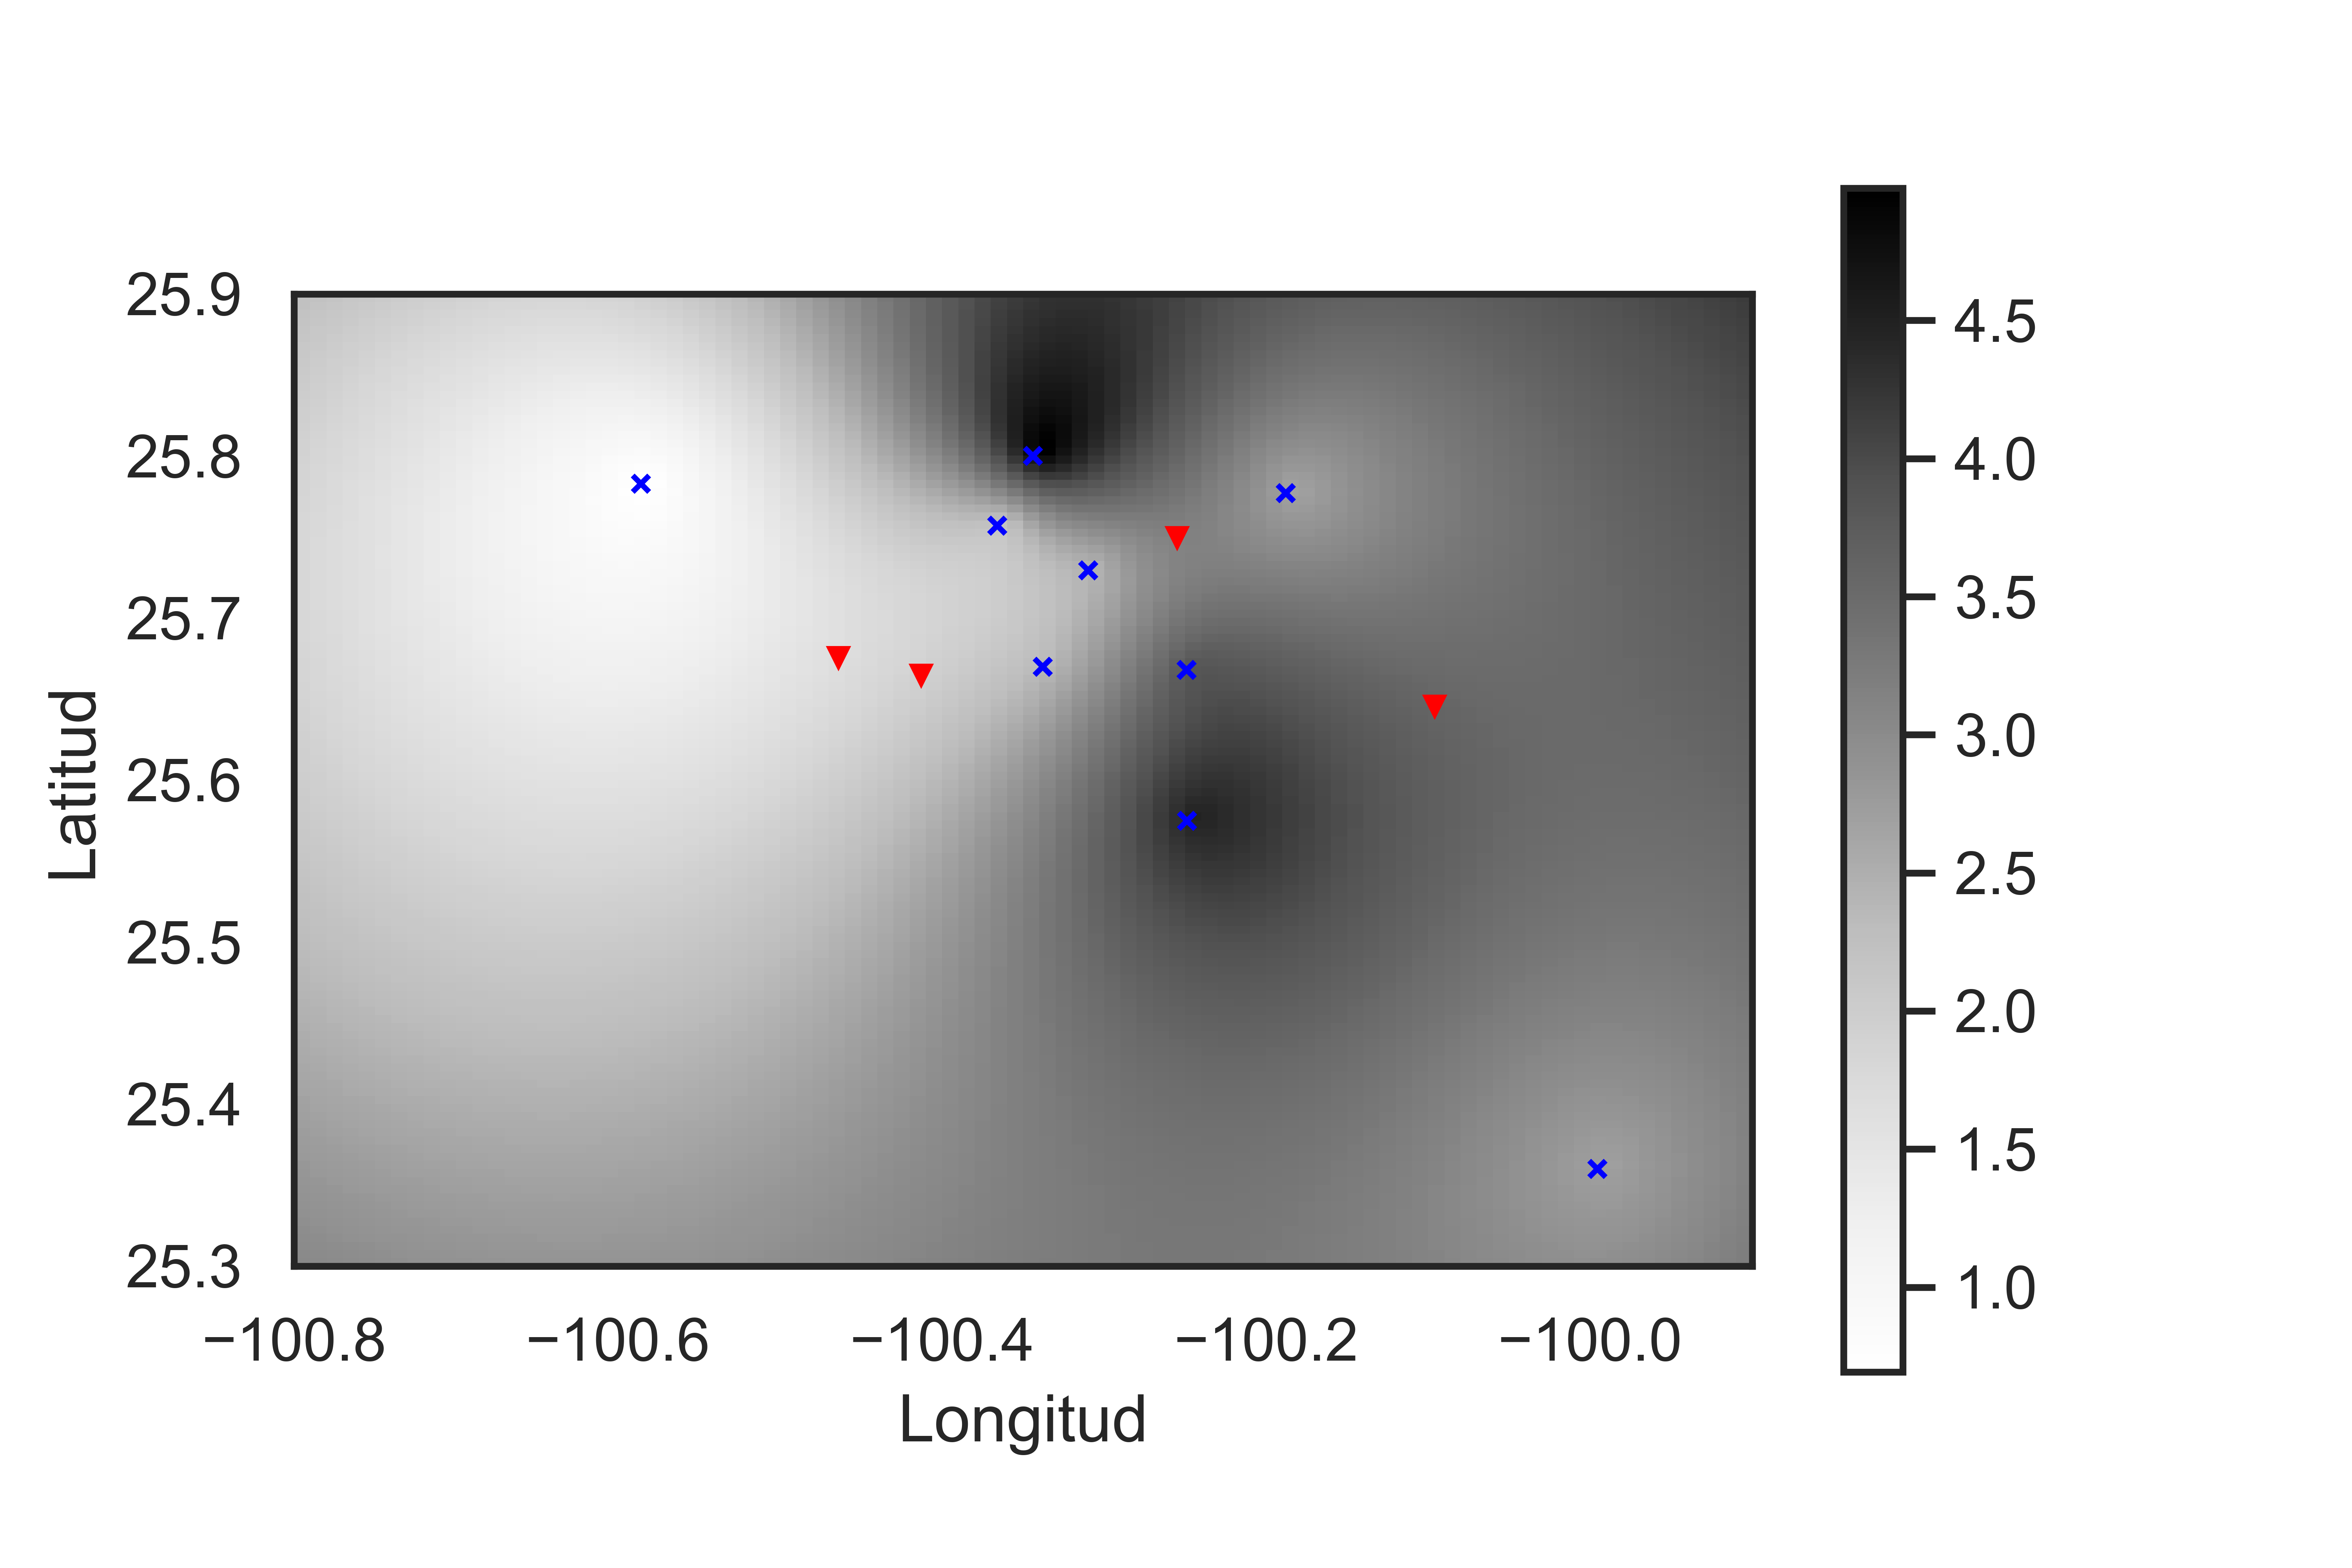
\includegraphics[width=4cm, height=4cm]{./brf_l_9_2_26302}}
\subfigure[FBR C] {\includegraphics[width=4cm, height=4cm]{./brf_c_9_2_26302}}
\subfigure[FBR Q] {\includegraphics[width=4cm, height=4cm]{./brf_q_9_2_26302}}
\subfigure[FBR TPS] {\includegraphics[width=4cm, height=4cm]{./brf_tps_9_2_26302}}
\subfigure[KO] {\includegraphics[width=4cm, height=4cm]{./ok_9_2_26302}}
\subfigure[KU] {\includegraphics[width=4cm, height=4cm]{./uk_9_2_26302}}
\caption{Interpolaciones de NO$_{2}$ para 9 estaciones seleccionadas y 4 estaciones interpoladas: Fecha (31-12-2018 23:00:00)}
\label{NO2figure1}
\end{figure}


\begin{table}[H]
\centering
\caption{NO$_{2}$: 10 estaciones seleccionadas 3 estaciones interpoladas}
\begin{adjustbox}{max width=0.9\textwidth}
\begin{tabular}{|c|c|c|c|c|c|c|}
\hline
\multicolumn{7}{ |c| }{Métricas de error} \\ \hline
Método &MAPE &MAE &MAEP &RMSE &RMSEP &MSE \\ \hline
TV &0.81 &6.05 &0.58 &9.45 &0.90 &89.38 \\
DIP &0.60 &4.46 &0.42 &7.57 &0.72 &57.32 \\
FBR M &$3.01\times10^{14}$ &$2.22\times10^{15}$ &$2.13\times10^{14}$ &$1.43\times10^{17}$ &$1.37\times10^{16}$ &$2.04\times10^{34}$ \\
FBR IM &0.85 &6.88 &0.66 &10.14 &0.97 &102.84 \\
FBR G &$1.32\times10^{14}$ &$4.67\times10^{14}$ &$4.49\times10^{13}$ &$6.56\times10^{16}$ &$6.31\times10^{15}$ &$4.31\times10^{33}$ \\
FBR L &1.87 &11.55 &1.11 &35.55 &3.42 &1,264.48 \\
FBR C &$1.00\times10^{17}$ &$5.51\times10^{17}$ &$5.30\times10^{16}$ &$2.25\times10^{18}$ &$2.16\times10^{17}$ &$5.08\times10^{36}$ \\
FBR Q &$2.50\times10^{17}$ &$1.55\times10^{18}$ &$1.49\times10^{17}$ &$3.77\times10^{18}$ &$3.63\times10^{17}$ &$1.42\times10^{37}$ \\
FBR TPS &1.70 &10.73 &1.03 &50.15 &4.82 &2,515.03 \\
KO &0.63 &4.62 &0.44 &7.84 &0.75 &61.55 \\
KU &0.81 &6.05 &0.58 &13.44 &1.29 &180.77 \\\hline
\end{tabular}
\end{adjustbox}
\label{tabNO2_2}
\end{table}


De la tabla \ref{tabNO2_2} en la cual se utilizan diez estaciones para interpolar otras tres, podemos ver que los métodos que obtiene peores resultados de predicción, son los métodos de Funciones de Base Radial, a excepción de los métodos inverso multicuadrático, lineal y {\em thin plate splines} (FBR I,  FBR L y FBR TPS), entre los métodos deterministas, el método DIP obtuvo el menor MAPE, MAE, MAEP, RMSE, RMSEP y MSE; mientras que de los métodos geoestadísticos el método KO obtuvo el menor MAPE, MAE, MAEP, RMSE, RMSEP y MSE. En general, DIP y KO son mejores que el resto de los métodos pero DIP es mejor que KO ya que en los errores MAPE, MAE, MAEP, RMSE RMSEP y MSE obtuvo mejores resultados que el método KO. En la figura \ref{NO2figure2}, se pueden observar las interpolaciones de cada método, donde las puntos azules son las estaciones seleccionadas y los puntos rojos son las estaciones interpoladas.


\begin{figure}[H]
\centering
\subfigure[TV] {\includegraphics[width=4cm, height=4cm]{./voronoi_10_2_26302}}
\subfigure[DIP] {\includegraphics[width=4cm, height=4cm]{./idw_10_2_26302}}
\subfigure[FBR M] {\includegraphics[width=4cm, height=4cm]{./brf_m_10_2_26302}}
\subfigure[FBR I] {\includegraphics[width=4cm, height=4cm]{./brf_i_10_2_26302}}
\subfigure[FBR G] {\includegraphics[width=4cm, height=4cm]{./brf_g_10_2_26302}}
\subfigure[FBR L] {\includegraphics[width=4cm, height=4cm]{./brf_l_10_2_26302}}
\subfigure[FBR C] {\includegraphics[width=4cm, height=4cm]{./brf_c_10_2_26302}}
\subfigure[FBR Q] {\includegraphics[width=4cm, height=4cm]{./brf_q_10_2_26302}}
\subfigure[FBR TPS] {\includegraphics[width=4cm, height=4cm]{./brf_tps_10_2_26302}}
\subfigure[KO] {\includegraphics[width=4cm, height=4cm]{./ok_10_2_26302}}
\subfigure[KU] {\includegraphics[width=4cm, height=4cm]{./uk_10_2_26302}}
\caption{Interpolaciones de NO$_{2}$ para 10 estaciones seleccionadas y 3 estaciones interpoladas: Fecha (31-12-2018 23:00:00)}
\label{NO2figure2}
\end{figure}


\begin{table}[H]
\centering
\caption{NO$_{2}$: 11 estaciones seleccionadas 2 estaciones interpoladas}
\begin{adjustbox}{max width=0.9\textwidth}
\begin{tabular}{|c|c|c|c|c|c|c|}
\hline
\multicolumn{7}{ |c| }{Métricas de error} \\ \hline
Método &MAPE &MAE &MAEP &RMSE &RMSEP &MSE \\ \hline
TV &0.82 &6.10 &0.58 &9.49 &0.91 &90.14 \\
DIP &0.60 &4.44 &0.42 &7.54 &0.72 &56.97 \\
FBR M &$2.66\times10^{14}$ &$1.92\times10^{15}$ &$1.85\times10^{14}$ &$1.33\times10^{17}$ &$1.28\times10^{16}$ &$1.7\times10^{34}$ \\
FBR IM &0.90 &7.09 &0.68 &10.34 &0.99 &107.03 \\
FBR G &$5.59\times10^{13}$ &$3.50\times10^{14}$ &$3.37\times10^{13}$ &$5.68\times10^{16}$ &$5.47\times10^{15}$ &$3.23\times10^{33}$ \\
FBR L &1.70 &10.38 &0.99 &26.98 &2.59 &728.01 \\
FBR C &$8.81\times10^{16}$ &$4.77\times10^{17}$ &$4.59\times10^{16}$ &$2.09\times10^{18}$ &$2.01\times10^{17}$ &$4.40\times10^{36}$ \\
FBR Q &$1.70\times10^{17}$ &$1.05\times10^{18}$ &$1.01\times10^{17}$ &$3.11\times10^{18}$ &$2.99\times10^{17}$ &$9.68\times10^{36}$ \\
FBR TPS &1.52 &9.56 &0.92 &35.03 &3.37 &1,227.34 \\
KO &0.629 &4.59 &0.44 &7.77 &0.74 &60.50 \\
KU &0.78 &5.78 &0.55 &11.58 &1.11 &134.26 \\\hline
\end{tabular}
\end{adjustbox}
\label{tabNO2_3}
\end{table}


De la tabla \ref{tabNO2_3}, en la cual se utilizan once estaciones para interpolar dos estaciones más, podemos ver que los métodos que obtiene peores resultados de predicción son los métodos de Funciones de Base Radial, a excepción de los métodos inverso multicuadrático, lineal y {\em thin plate splines} (FBR I,  FBR L y FBR TPS); entre los métodos deterministas, DIP obtuvo el menor MAPE, MAE, MAEP, RMSE, RMSEP y MSE, mientras que de los métodos geoestadísticos el método KO obtuvo el menor MAPE, MAE, MAEP, RMSE, RMSEP y MSE. En general, DIP y KO son mejores que el resto de los métodos, pero DIP es mejor que KO ya que en todos los errores son menores a los errores de KO. En la figura \ref{NO2figure3}, se pueden observar las interpolaciones de cada método, donde las puntos azules son las estaciones seleccionadas y los puntos rojos son las estaciones interpoladas.


\begin{figure}[H]
\centering
\subfigure[TV] {\includegraphics[width=4cm, height=4cm]{./voronoi_11_2_26302}}
\subfigure[DIP] {\includegraphics[width=4cm, height=4cm]{./idw_11_2_26302}}
\subfigure[FBR M] {\includegraphics[width=4cm, height=4cm]{./brf_m_11_2_26302}}
\subfigure[FBR I] {\includegraphics[width=4cm, height=4cm]{./brf_i_11_2_26302}}
\subfigure[FBR G] {\includegraphics[width=4cm, height=4cm]{./brf_g_11_2_26302}}
\subfigure[FBR L] {\includegraphics[width=4cm, height=4cm]{./brf_l_11_2_26302}}
\subfigure[FBR C] {\includegraphics[width=4cm, height=4cm]{./brf_c_11_2_26302}}
\subfigure[FBR Q] {\includegraphics[width=4cm, height=4cm]{./brf_q_11_2_26302}}
\subfigure[FBR TPS] {\includegraphics[width=4cm, height=4cm]{./brf_tps_11_2_26302}}
\subfigure[KO] {\includegraphics[width=4cm, height=4cm]{./ok_11_2_26302}}
\subfigure[KU] {\includegraphics[width=4cm, height=4cm]{./uk_11_2_26302}}
\caption{Interpolaciones de NO$_{2}$ para 11 estaciones seleccionadas y 2 estaciones interpoladas: Fecha (31-12-2018 23:00:00)}
\label{NO2figure3}
\end{figure}


\begin{table}[H]
\centering
\caption{NO$_{2}$: 12 estaciones seleccionadas 1 estación interpolada}
\begin{adjustbox}{max width=0.9\textwidth}
\begin{tabular}{|c|c|c|c|c|c|c|}
\hline
\multicolumn{7}{ |c| }{Métricas de error} \\ \hline
Método &MAPE &MAE &MAEP &RMSE &RMSEP &MSE \\ \hline
TV &0.82 &6.11 &0.58 &9.44 &0.90 &89.19 \\
DIP &0.59 &4.42 &0.42 &7.53 &0.72 &56.79 \\
FBR M &$2.52\times10^{14}$ &$2.80\times10^{15}$ &$2.68\times10^{14}$ &$1.60\times10^{17}$ &$1.53\times10^{16}$ &$2.58\times10^{34}$ \\
FBR IM &0.93 &7.30 &0.69 &10.43 &0.99 &108.96 \\
FBR G &1.20 &10.27 &0.98 &19.31 &1.84 &373.16 \\
FBR L &1.54 &9.48 &0.90 &19.73 &1.88 &389.62 \\
FBR C &$7.40\times10^{16}$ &$4.32\times10^{17}$ &$4.14\times10^{16}$ &$1.99\times10^{18}$ &$1.91\times10^{17}$ &$3.99\times10^{36}$ \\
FBR Q &$1.20\times10^{17}$ &$8.15\times10^{17}$ &$7.80\times10^{16}$ &$2.74\times10^{18}$ &$2.62\times10^{17}$ &$7.51\times10^{36}$ \\
FBR TPS &1.30 &8.38 &0.80 &16.85 &1.61 &284.10 \\
KO &0.61 &4.57 &0.43 &7.76 &0.74 &60.24 \\
KU &0.74 &5.65 &0.54 &10.42 &0.99 &108.76 \\\hline
\end{tabular}
\end{adjustbox}
\label{tabNO2_4}
\end{table}

De la tabla \ref{tabNO2_4}, en la cual se utilizan doce estaciones para interpolar una estación, podemos ver que los métodos que obtiene peores resultados de predicción son los métodos de Funciones de Base Radial, a excepción de los métodos inverso multicuadrático, lineal y {\em thin plate splines} (FBR I,  FBR L y FBR TPS); entre los métodos deterministas, DIP obtuvo el menor MAPE, MAE, MAEP, RMSE, RMSEP y MSE, mientras que de los métodos geoestadísticos el método KO obtuvo el menor MAPE, MAE, MAEP, RMSE, RMSEP y MSE. Los métodos DIP y KO son mejores que el resto de los métodos, pero DIP es mejor que KO ya que todos los errores encontrados por DIP son menores a los errores encontrados por KO. En la figura \ref{NO2figure4}, se pueden observar las interpolaciones de cada método, donde las puntos azules son las estaciones seleccionadas y los puntos rojos son las estaciones interpoladas. En general, mientras se aumenta el número de estaciones para interpolar la variable NO$_{2}$, éstas bajan de forma rápida sus errores en algunos métodos como las funciones de base radial y para el resto de los metodos que ya son buenos para interpolar también mejoran pero los cambios ya son con menor intensidad.



\begin{figure}[H]
\centering
\subfigure[TV] {\includegraphics[width=4cm, height=4cm]{./voronoi_12_2_26302}}
\subfigure[DIP] {\includegraphics[width=4cm, height=4cm]{./idw_12_2_26302}}
\subfigure[FBR M] {\includegraphics[width=4cm, height=4cm]{./brf_m_12_2_26302}}
\subfigure[FBR I] {\includegraphics[width=4cm, height=4cm]{./brf_i_12_2_26302}}
\subfigure[FBR G] {\includegraphics[width=4cm, height=4cm]{./brf_g_12_2_26302}}
\subfigure[FBR L] {\includegraphics[width=4cm, height=4cm]{./brf_l_12_2_26302}}
\subfigure[FBR C] {\includegraphics[width=4cm, height=4cm]{./brf_c_12_2_26302}}
\subfigure[FBR Q] {\includegraphics[width=4cm, height=4cm]{./brf_q_12_2_26302}}
\subfigure[FBR TPS] {\includegraphics[width=4cm, height=4cm]{./brf_tps_12_2_26302}}
\subfigure[KO] {\includegraphics[width=4cm, height=4cm]{./ok_12_2_26302}}
\subfigure[KU] {\includegraphics[width=4cm, height=4cm]{./uk_12_2_26302}}
\caption{Interpolaciones de NO$_{2}$ para 12 estaciones seleccionadas y 1 estación interpolada: Fecha (31-12-2018 23:00:00)}
\label{NO2figure4}
\end{figure}





\subsection{Ozono (O$_{3}$)}

\begin{table}[H]
\centering
\caption{O$_{3}$:  9 estaciones seleccionadas 4 estaciones interpoladas}
\begin{adjustbox}{max width=0.9\textwidth}
\begin{tabular}{|c|c|c|c|c|c|c|}
\hline
\multicolumn{7}{ |c| }{Métricas de error} \\ \hline
Método &MAPE &MAE &MAEP &RMSE &RMSEP &MSE \\ \hline
TV &0.69 &11.28 &0.44 &17.26 &0.67 &298.22 \\
DIP &0.49 &7.95 &0.31 &13.01 &0.50 &169.37 \\
FBR M &$5.53\times10^{13}$ &$5.39\times10^{16}$ &$2.11\times10^{15}$ &$7.05\times10^{17}$ &$2.76\times10^{16}$ &$4.97\times10^{35}$ \\
FBR IM &$5.66 \times10^{14}$ &$5.61\times10^{15}$ &$2.19\times10^{14}$ &$2.27\times10^{17}$ &$8.90\times10^{15}$ &$5.17\times10^{34}$ \\
FBR G &$7.32\times10^{15}$ &$6.20\times10^{16}$ &$2.42\times10^{15}$ &$7.56\times10^{17}$ &$2.96\times10^{16}$ &$5.72\times10^{35}$ \\
FBR L &1.21 &23.71 &0.92 &58.65 &2.29 &3,440.80 \\
FBR C &$5.96\times10^{16}$ &$9.94\times10^{17}$ &$3.89\times10^{16}$ &$3.02\times10^{18}$ &$1.18\times10^{17}$ &$9.17\times10^{36}$ \\
FBR Q &$1.50\times10^{17}$ &$1.95\times10^{18}$ &$7.67\times10^{16}$ &$4.25\times10^{18}$ &$1.66\times10^{17}$ &$1.80\times10^{37}$ \\
FBR TPS &$43.01\times10^{12}$ &$5.25\times10^{14}$ &$2.05\times10^{13}$ &$6.96\times10^{16}$ &$2.72\times10^{13}$ &$4.85\times^{33}$ \\
KO &0.51 &8.17 &0.32 &3.37 &0.52 &178.88 \\
KU &$1.18\times10^{13}$ &$1.30\times10^{16}$ &$5.11\times10^{14}$ &$3.47\times10^{17}$ &$1.35\times10^{16}$ &$1.20\times10^{35}$ \\\hline
\end{tabular}
\end{adjustbox}
\label{tabO3}
\end{table}


De la tabla \ref{tabO3}, en la cual se utilizan nueve estaciones para interpolar cuatro más, podemos ver que los métodos que obtiene peores resultados de predicción son los métodos de Funciones de Base Radial, a excepción de los método lineal (FBR L), entre los métodos deterministas el método DIP obtuvo el menor MAPE, MAE, MAEP, RMSE, RMSEP y MSE, mientras que de los métodos geoestadísticos, el método KO obtuvo el menor MAPE, MAE, MAEP, RMSE, RMSEP y MSE. En general, DIP y KO son mejores que el resto de los métodos pero DIP es mejor que KO ya que en todos los errores a excepción de RMSE obtuvo mejores resultados que los errores de KO. En la figura \ref{O3figure1}, se pueden observar las interpolaciones de cada método, donde las puntos azules son las estaciones seleccionadas y los puntos rojos son las estaciones interpoladas.

\begin{figure}[H]
\centering
\subfigure[TV] {\includegraphics[width=4cm, height=4cm]{./voronoi_9_4_26302}}
\subfigure[DIP] {\includegraphics[width=4cm, height=4cm]{./idw_9_4_26302}}
\subfigure[FBR M] {\includegraphics[width=4cm, height=4cm]{./brf_m_9_4_26302}}
\subfigure[FBR I] {\includegraphics[width=4cm, height=4cm]{./brf_i_9_4_26302}}
\subfigure[FBR G] {\includegraphics[width=4cm, height=4cm]{./brf_g_9_4_26302}}
\subfigure[FBR L] {\includegraphics[width=4cm, height=4cm]{./brf_l_9_4_26302}}
\subfigure[FBR C] {\includegraphics[width=4cm, height=4cm]{./brf_c_9_4_26302}}
\subfigure[FBR Q] {\includegraphics[width=4cm, height=4cm]{./brf_q_9_4_26302}}
\subfigure[FBR TPS] {\includegraphics[width=4cm, height=4cm]{./brf_tps_9_4_26302}}
\subfigure[KO] {\includegraphics[width=4cm, height=4cm]{./ok_9_4_26302}}
\subfigure[KU] {\includegraphics[width=4cm, height=4cm]{./uk_9_4_26302}}
\caption{Interpolaciones de O$_{3}$ para 9 estaciones seleccionadas y 4 estaciones interpoladas: Fecha (31-12-2018 23:00:00)}
\label{O3figure1}
\end{figure}


\begin{table}[H]
\centering
\caption{O$_{3}$:  10 estaciones seleccionadas 3 estaciones interpoladas}
\begin{adjustbox}{max width=0.9\textwidth}
\begin{tabular}{|c|c|c|c|c|c|c|}
\hline
\multicolumn{7}{ |c| }{Métricas de error} \\ \hline
Método &MAPE &MAE &MAEP &RMSE &RMSEP &MSE \\ \hline
TV &0.69 &11.43 &0.44 &17.52 &0.68 &307.02 \\
DIP &0.48 &7.91 &0.30 &13.01 &0.50 &169.39 \\
FBR M &$5.85\times10^{15}$ &$5.76\times10^{16}$ &$2.25\times10^{15}$ &$7.29\times10^{17}$ &$2.85\times10^{16}$ &$5.31\times10^{35}$ \\
FBR IM &$3.87\times10^{14}$ &$4.44\times10^{15}$ &$1.73\times10^{14}$ &$2.02\times10^{17}$ &$791\times10^{13}$ &$4.09\times10^{34}$ \\
FBR G &$8.71\times10^{15}$ &$7.67\times10^{16}$ &$3.00\times10^{15}$ &$8.41\times10^{17}$ &$3.29\times10^{16}$ &$7.08\times10^{35}$ \\
FBR L &1.09 &20.95 &0.81 &46.95 &1.83 &2,204.98 \\
FBR C &$5.33\times10^{16}$ &$8.96\times10^{17}$ &$3.50\times10^{16}$ &$2.87\times10^{18}$ &$1.12\times10^{17}$ &$8.26\times10^{36}$ \\
FBR Q &$1.41\times10^{17}$ &$1.71\times10^{18}$ &$6.69\times10^{16}$ &$3.97\times10^{18}$ &$1.55\times10^{17}$ &$1.57\times10^{37}$ \\
FBR TPS &$3.01\times10^{13}$ &$5.84\times10^{13}$ &$2.28\times10^{13}$ &$7.34\times10^{16}$ &$2.87\times10^{15}$ &$5.39\times10^{33}$ \\
KO &0.50 &8.12 &0.31 &13.36 &0.52 &178.62 \\
KU &$1.03\times10^{15}$ &$1.22\times10^{16}$ &$4.79\times10^{14}$ &$3.36\times10^{17}$ &$1.31\times10^{16}$ &$1.13\times10^{35}$ \\\hline
\end{tabular}
\end{adjustbox}
\label{tabO3_2}
\end{table}


De la tabla \ref{tabO3_2}, en la cual se utilizan diez estaciones para interpolar tres estaciones, podemos ver que los métodos que obtiene peores resultados de predicción son los métodos de Funciones de Base Radial, a excepción de los método lineal (FBR L), entre los métodos deterministas el método DIP obtuvo el menor MAPE, MAE, MAEP, RMSE, RMSEP y MSE; mientras que de los métodos geoestadísticos el método KO obtuvo el menor MAPE, MAE, MAEP, RMSE, RMSEP y MSE, en general DIP y KO son mejores que el resto de los métodos pero DIP es mejor que KO, pues en todos los errores encontrados por DIP son menores a los errores de KO. En la figura \ref{O3figure2} se pueden observar las interpolaciones de cada método, donde las puntos azules son las estaciones seleccionadas y los puntos rojos son las estaciones interpoladas.


\begin{figure}[H]
\centering
\subfigure[TV] {\includegraphics[width=4cm, height=4cm]{./voronoi_10_4_26302}}
\subfigure[DIP] {\includegraphics[width=4cm, height=4cm]{./idw_10_4_26302}}
\subfigure[FBR M] {\includegraphics[width=4cm, height=4cm]{./brf_m_10_4_26302}}
\subfigure[FBR I] {\includegraphics[width=4cm, height=4cm]{./brf_i_10_4_26302}}
\subfigure[FBR G] {\includegraphics[width=4cm, height=4cm]{./brf_g_10_4_26302}}
\subfigure[FBR L] {\includegraphics[width=4cm, height=4cm]{./brf_l_10_4_26302}}
\subfigure[FBR C] {\includegraphics[width=4cm, height=4cm]{./brf_c_10_4_26302}}
\subfigure[FBR Q] {\includegraphics[width=4cm, height=4cm]{./brf_q_10_4_26302}}
\subfigure[FBR TPS] {\includegraphics[width=4cm, height=4cm]{./brf_tps_10_4_26302}}
\subfigure[KO] {\includegraphics[width=4cm, height=4cm]{./ok_10_4_26302}}
\subfigure[KU] {\includegraphics[width=4cm, height=4cm]{./uk_10_4_26302}}
\caption{Interpolaciones de O$_{3}$ para 10 estaciones seleccionadas y 3 estaciones interpoladas: Fecha (31-12-2018 23:00:00)}
\label{O3figure2}
\end{figure}


\begin{table}[H]
\centering
\caption{O$_{3}$:  11 estaciones seleccionadas 2 estaciones interpoladas}
\begin{adjustbox}{max width=0.9\textwidth}
\begin{tabular}{|c|c|c|c|c|c|c|}
\hline
\multicolumn{7}{ |c| }{Métricas de error} \\ \hline
Método &MAPE &MAE &MAEP &RMSE &RMSEP &MSE \\ \hline
TV &0.70 &11.48 &0.44 &17.64 &0.69 &311.32 \\
DIP &0.48 &7.86 &0.30 &12.94 &0.50 &167.62 \\
FBR M &$4.30\times10^{15}$ &$5.39\times10^{16}$ &$2.11\times10^{15}$ &$7.05\times10^{17}$ &$2.76\times10^{16}$ &$4.98\times10^{35}$ \\
FBR IM &$3.30\times10^{15}$ &$3.85\times10^{15}$ &$1.50\times10^{14}$ &$1.88\times10^{17}$ &$7.37\times10^{15}$ &$3.55\times10^{34}$ \\
FBR G &$9.63\times10^{15}$ &$9.11\times10^{16}$ &$3.56\times10^{15}$ &$9.16\times10^{17}$ &$3.58\times10^{16}$ &$8.40\times10^{35}$ \\
FBR L &1.034 &19.85 &0.77 &42.77 &1.67 &1,829.37 \\
FBR C &$4.65\times10^{16}$ &$8.23\times10^{17}$ &$3.22\times10^{16}$ &$2.75\times10^{18}$ &$1.07\times10^{17}$ &$7.59\times10^{36}$ \\
FBR Q &$1.00\times10^{17}$ &$1.18\times10^{18}$ &$4.64\times10^{16}$ &$3.31\times10^{18}$ &$1.29\times10^{17}$ &$1.09\times10^{37}$ \\
FBR TPS &$2.55\times10^{13}$ &$3.50\times10^{14}$ &$1.37\times10^{13}$ &$5.68\times10^{16}$ &$2.22\times10^{15}$ &$3.23\times10^{33}$ \\
KO &0.50 &8.061 &0.315 &13.27 &0.519 &176.16 \\
KU &$8.86\times10^{14}$ &$1.06\times10^{16}$ &$4.18\times10^{14}$ &$3.14\times10^{17}$ &$1.22\times10^{16}$ &$9.86\times10^{34}$ \\\hline
\end{tabular}
\end{adjustbox}
\label{tabO3_3}
\end{table}


De la tabla \ref{tabO3_3}, en la cual se utilizan once estaciones para interpolar dos más, podemos ver que los métodos que obtiene peores resultados de predicción son los métodos de Funciones de Base Radial, a excepción de los método lineal (FBR L), entre los métodos deterministas el método DIP obtuvo el menor MAPE, MAE, MAEP, RMSE, RMSEP y MSE; mientras que de los métodos geoestadísticos el método KO obtuvo el menor MAPE, MAE, MAEP, RMSE, RMSEP y MSE, en general DIP y KO son mejores que el resto de los métodos pero DIP es mejor que KO ya que en todos los errores son menores a los errores de KO. En la figura \ref{O3figure3}, se pueden observar las interpolaciones de cada método, donde las puntos azules son las estaciones seleccionadas y los puntos rojos son las estaciones interpoladas.


\begin{figure}[H]
\centering
\subfigure[TV] {\includegraphics[width=4cm, height=4cm]{./voronoi_11_4_26302}}
\subfigure[DIP] {\includegraphics[width=4cm, height=4cm]{./idw_11_4_26302}}
\subfigure[FBR M] {\includegraphics[width=4cm, height=4cm]{./brf_m_11_4_26302}}
\subfigure[FBR I] {\includegraphics[width=4cm, height=4cm]{./brf_i_11_4_26302}}
\subfigure[FBR G] {\includegraphics[width=4cm, height=4cm]{./brf_g_11_4_26302}}
\subfigure[FBR L] {\includegraphics[width=4cm, height=4cm]{./brf_l_11_4_26302}}
\subfigure[FBR C] {\includegraphics[width=4cm, height=4cm]{./brf_c_11_4_26302}}
\subfigure[FBR Q] {\includegraphics[width=4cm, height=4cm]{./brf_q_11_4_26302}}
\subfigure[FBR TPS] {\includegraphics[width=4cm, height=4cm]{./brf_tps_11_4_26302}}
\subfigure[KO] {\includegraphics[width=4cm, height=4cm]{./ok_11_4_26302}}
\subfigure[KU] {\includegraphics[width=4cm, height=4cm]{./uk_11_4_26302}}
\caption{Interpolaciones de O$_{3}$ para 11 estaciones seleccionadas y 2 estaciones interpoladas: Fecha (31-12-2018 23:00:00)}
\label{O3figure3}
\end{figure}



\begin{table}[H]
\centering
\caption{O$_{3}$: 12 estaciones seleccionadas 1 estación interpolada}
\begin{adjustbox}{max width=0.9\textwidth}
\begin{tabular}{|c|c|c|c|c|c|c|}
\hline
\multicolumn{7}{ |c| }{Métricas de error} \\ \hline
Método &MAPE &MAE &MAEP &RMSE &RMSEP &MSE \\ \hline
TV &0.72 &11.71 &0.46 &18.03 &0.70 &325.16 \\
DIP &0.48 &7.80 &0.30 &12.92 &0.50 &167.16 \\
FBR M &$4.13\times10^{15}$ &$5.54\times10^{16}$ &$2.17\times10^{15}$ &$7.14\times10^{17}$ &$2.81\times10^{16}$ &$5.10\times10^{35}$ \\
FBR IM &$7.22\times10^{14}$ &$7.36\times10^{15}$ &$2.89\times10^{14}$ &$2.60\times10^{17}$ &$1.02\times10^{16}$ &$6.79\times10^{34}$ \\
FBR G &$1.31\times10^{16}$ &$1.38\times10^{17}$ &$5.44\times10^{15}$ &$1.13\times10^{18}$ &$4.44\times10^{16}$ &$1.27\times10^{36}$ \\
FBR L &0.99 &18.76 &0.73 &38.54 &1.51 &1,485.79 \\
FBR C &$4.38\times10^{16}$ &$7.94\times10^{17}$ &$3.12\times10^{16}$ &$2.70\times10^{18}$ &$1.06\times10^{17}$ &$7.32\times10^{36}$ \\
FBR Q &$6.95\times10^{16}$ &$8.07\times10^{17}$ &$3.17\times10^{16}$ &$2.72\times10^{18}$ &$1.07\times10^{17}$ &$7.44\times10^{36}$ \\
FBR TPS &0.91 &15.56 &0.61 &29.04 &1.14 &843.58 \\
KO &0.50 &7.97 &0.31 &13.18 &0.51 &173.73 \\
KU &$9.14\times10^{14}$ &$1.05\times10^{16}$ &$4.13\times10^{14}$ &$3.11\times10^{17}$ &$1.22\times10^{16}$ &$9.70\times10^{34}$ \\\hline
\end{tabular}
\end{adjustbox}
\label{tabO3_4}
\end{table}

De la tabla \ref{tabO3_4}, en la cual se utilizan doce estaciones para interpolar una estación más, podemos ver que los métodos que obtiene peores resultados de predicción son los métodos de Funciones de Base Radial, a excepción de los métodos lineal y thin plate splines (FBR L y FBR TPS); entre los métodos deterministas, DIP obtuvo el menor MAPE, MAE, MAEP, RMSE, RMSEP y MSE, mientras que de los métodos geoestadísticos el método KO obtuvo el menor MAPE, MAE, MAEP, RMSE, RMSEP y MSE. Los métodos DIP y KO son mejores que el resto de los métodos pero DIP es mejor que KO ya que en todos los errores obtenidos por DIP son menores que los errores de KO. En la figura \ref{O3figure4}, se pueden observar las interpolaciones de cada método, donde las puntos azules son las estaciones seleccionadas y los puntos rojos son las estaciones interpoladas. En general, mientras se aumenta el número de estaciones para interpolar la variable O$_{3}$, éstas bajan de forma rápida sus errores en algunos métodos como las funciones de base radial y para el resto de los métodos que ya son buenos para interpolar también mejoran pero los cambios ya son con menor intensidad.


\begin{figure}[H]
\centering
\subfigure[TV] {\includegraphics[width=4cm, height=4cm]{./voronoi_12_4_26302}}
\subfigure[DIP] {\includegraphics[width=4cm, height=4cm]{./idw_12_4_26302}}
\subfigure[FBR M] {\includegraphics[width=4cm, height=4cm]{./brf_m_12_4_26302}}
\subfigure[FBR I] {\includegraphics[width=4cm, height=4cm]{./brf_i_12_4_26302}}
\subfigure[FBR G] {\includegraphics[width=4cm, height=4cm]{./brf_g_12_4_26302}}
\subfigure[FBR L] {\includegraphics[width=4cm, height=4cm]{./brf_l_12_4_26302}}
\subfigure[FBR C] {\includegraphics[width=4cm, height=4cm]{./brf_c_12_4_26302}}
\subfigure[FBR Q] {\includegraphics[width=4cm, height=4cm]{./brf_q_12_4_26302}}
\subfigure[FBR TPS] {\includegraphics[width=4cm, height=4cm]{./brf_tps_12_4_26302}}
\subfigure[KO] {\includegraphics[width=4cm, height=4cm]{./ok_12_4_26302}}
\subfigure[KU] {\includegraphics[width=4cm, height=4cm]{./uk_12_4_26302}}
\caption{Interpolaciones de O$_{3}$ para 12 estaciones seleccionadas y 1 estación interpolada: Fecha (31-12-2018 23:00:00)}
\label{O3figure4}
\end{figure}





\subsection{Partículas Menores a 10 Micras (PM$_{10}$)}

\begin{table}[H]
\centering
\caption{PM$_{10}$: 9 estaciones seleccionadas 4 estaciones interpoladas}
\begin{adjustbox}{max width=0.9\textwidth}
\begin{tabular}{|c|c|c|c|c|c|c|}
\hline
\multicolumn{7}{ |c| }{Métricas de error} \\ \hline
Método &MAPE &MAE &MAEP &RMSE &RMSEP &MSE \\ \hline
TV &0.53 &26.72 &0.44 &44.30 &0.73 &1,963.15 \\
DIP &0.39 &19.11 &0.31 &32.78 &0.54 &1,074.85 \\
FBR M &$1.70\times10^{12}$ &$3.94\times10^{13}$ &$6,50\times10^{11}$ &$1.90\times10^{17}$ &$3.14\times10^{13}$ &$3.63\times10^{34}$ \\
FBR IM &0.66 &33.85 &0.55 &58.90 &0.97 &3,470.28 \\
FBR G &$1.83\times10^{12}$ &$4.82\times10^{13}$ &$7.95\times10^{11}$ &$2.10\times10^{17}$ &$3.47\times10^{13}$ &$4.44\times10^{34}$ \\
FBR L &2.28 &118.00 &1.94 &527.01 &8.69 &277,744.08 \\
FBR C &$2.68\times10^{16}$ &$9.91\times10^{17}$ &$1.63\times10^{16}$ &$3.02\times10^{18}$ &$4.98\times10^{16}$ &$9.14\times10^{36}$ \\
FBR Q &$4.76\times10^{16}$ &$1.72\times10^{18}$ &$2.85\times10^{16}$ &$3.98\times10^{18}$ &$6.57\times10^{16}$ &$1.58\times10^{37}$ \\
FBR TPS &1.30 &63.84 &1.05 &366.53 &6.04 &134,350.51 \\
KO &0.38 &19.44 &0.32 &33.35 &0.55 &1,112.30 \\
KU &0.48 &24.23 &0.39 &42.66 &0.70 &1,820.70 \\\hline
\end{tabular}
\end{adjustbox}
\label{tabPM10}
\end{table}

De la tabla \ref{tabPM10}, en la cual se utilizan nueve estaciones para interpolar otras cuatro, podemos ver que los métodos que obtiene peores resultados de predicción son los métodos de Funciones de Base Radial, a excepción de los métodos inverso multicuadrático lineal, {\em thin plate splines} (FBR IM, FBR L y FBR TPS); entre los métodos deterministas el método DIP obtuvo el menor MAPE, MAE, MAEP, RMSE, RMSEP y MSE, mientras que de los métodos geoestadísticos el método KO obtuvo el menor MAPE, MAE, MAEP, RMSE, RMSEP y MSE, en general DIP y KO son mejores que el resto de los métodos pero DIP es mejor que KO ya que en todos los errores son menores a los errores de KO a excepción del RMSE donde KO es menor a DIP. En la figura \ref{PM10figure1}, se pueden observar las interpolaciones de cada método, donde las puntos azules son las estaciones seleccionadas y los puntos rojos son las estaciones interpoladas.

\begin{figure}[H]
\centering
\subfigure[TV] {\includegraphics[width=4cm, height=4cm]{./voronoi_9_5_26302}}
\subfigure[DIP] {\includegraphics[width=4cm, height=4cm]{./idw_9_5_26302}}
\subfigure[FBR M] {\includegraphics[width=4cm, height=4cm]{./brf_m_9_5_26302}}
\subfigure[FBR I] {\includegraphics[width=4cm, height=4cm]{./brf_i_9_5_26302}}
\subfigure[FBR G] {\includegraphics[width=4cm, height=4cm]{./brf_g_9_5_26302}}
\subfigure[FBR L] {\includegraphics[width=4cm, height=4cm]{./brf_l_9_5_26302}}
\subfigure[FBR C] {\includegraphics[width=4cm, height=4cm]{./brf_c_9_5_26302}}
\subfigure[FBR Q] {\includegraphics[width=4cm, height=4cm]{./brf_q_9_5_26302}}
\subfigure[FBR TPS] {\includegraphics[width=4cm, height=4cm]{./brf_tps_9_5_26302}}
\subfigure[KO] {\includegraphics[width=4cm, height=4cm]{./ok_9_5_26302}}
\subfigure[KU] {\includegraphics[width=4cm, height=4cm]{./uk_9_5_26302}}
\caption{Interpolaciones de PM$_{10}$ para 9 estaciones seleccionadas y 4 estaciones interpoladas: Fecha (31-12-2018 23:00:00)}
\label{PM10figure1}
\end{figure}



\begin{table}[H]
\centering
\caption{PM$_{10}$: 10 estaciones seleccionadas 3 estaciones interpoladas}
\begin{adjustbox}{max width=0.9\textwidth}
\begin{tabular}{|c|c|c|c|c|c|c|}
\hline
\multicolumn{7}{ |c| }{Métricas de error} \\ \hline
Método &MAPE &MAE &MAEP &RMSE &RMSEP &MSE \\ \hline
TV &0.52 &26.64 &0.43 &44.14 &0.72 &1,949.08 \\
DIP &0.39 &18.92 &0.31 &32.66 &0.53 &1,067.22 \\
FBR M &$2.71\times10^{14}$ &$5.96\times10^{15}$ &$9.82\times10^{13}$ &$2.34\times10^{17}$ &$3.86\times10^{15}$ &$5.49\times10^{34}$ \\
FBR IM &0.68 &34.40 &0.56 &59.96 &0.98 &3,595.99 \\
FBR G &$1.44\times10^{14}$ &$4.55\times10^{15}$ &$7.51\times10^{13}$ &$2.05\times10^{17}$ &$3.37\times10^{15}$ &$4.20\times10^{34}$ \\
FBR L &1.8 &96.12 &1.58 &389.29 &6.41 &151546.85 \\
FBR C &$2.27\times10^{16}$ &$8.73\times10^{17}$ &$1.43\times10^{16}$ &$2.83\times10^{18}$ &$4.67\times10^{16}$ &$8.05\times10^{36}$ \\
FBR Q &$4.15\times10^{16}$ &$1.47\times10^{18}$ &$42.42\times10^{16}$ &$3.67\times10^{18}$ &$6.06\times10^{16}$ &$1.35\times10^{37}$ \\
FBR TPS &1.1 &53.83 &0.88 &300.63 &4.95 &90,383.85 \\
KO &0.38 &19.20 &0.31 &33.06 &0.54 &1,092.97 \\
KU &0.47 &23.43 &0.38 &41.41 &0.68 &1,715.16 \\\hline
\end{tabular}
\end{adjustbox}
\label{tabPM10_2}
\end{table}

De la tabla \ref{tabPM10_2}, en la cual se utilizan diez estaciones para interpolar tres más, podemos ver que los métodos que obtiene peores resultados de predicción son los métodos de Funciones de Base Radial, a excepción de los métodos inverso multicuadrático lineal, {\em thin plate splines} (FBR IM, FBR L y FBR TPS); entre los métodos deterministas el método DIP obtuvo el menor MAPE, MAE, MAEP, RMSE, RMSEP y MSE, mientras que de los métodos geoestadísticos el método KO obtuvo el menor MAPE, MAE, MAEP, RMSE, RMSEP y MSE. En general, DIP y KO son mejores que el resto de los métodos pero DIP es mejor que KO, pues en los errores MAE RMSEP y MSE obtuvo mejores resultados que KO. En la figura \ref{PM10figure2}, se pueden observar las interpolaciones de cada método, donde las puntos azules son las estaciones seleccionadas y los puntos rojos son las estaciones interpoladas.

 
\begin{figure}[H]
\centering
\subfigure[TV] {\includegraphics[width=4cm, height=4cm]{./voronoi_10_5_26302}}
\subfigure[DIP] {\includegraphics[width=4cm, height=4cm]{./idw_10_5_26302}}
\subfigure[FBR M] {\includegraphics[width=4cm, height=4cm]{./brf_m_10_5_26302}}
\subfigure[FBR I] {\includegraphics[width=4cm, height=4cm]{./brf_i_10_5_26302}}
\subfigure[FBR G] {\includegraphics[width=4cm, height=4cm]{./brf_g_10_5_26302}}
\subfigure[FBR L] {\includegraphics[width=4cm, height=4cm]{./brf_l_10_5_26302}}
\subfigure[FBR C] {\includegraphics[width=4cm, height=4cm]{./brf_c_10_5_26302}}
\subfigure[FBR Q] {\includegraphics[width=4cm, height=4cm]{./brf_q_10_5_26302}}
\subfigure[FBR TPS] {\includegraphics[width=4cm, height=4cm]{./brf_tps_10_5_26302}}
\subfigure[KO] {\includegraphics[width=4cm, height=4cm]{./ok_10_5_26302}}
\subfigure[KU] {\includegraphics[width=4cm, height=4cm]{./uk_10_5_26302}}
\caption{Interpolaciones de PM$_{10}$ para 10 estaciones seleccionadas y 3 estaciones interpoladas: Fecha (31-12-2018 23:00:00)}
\label{PM10figure2}
\end{figure}


\begin{table}[H]
\centering
\caption{PM$_{10}$: 11 estaciones seleccionadas 2 estaciones interpoladas}
\begin{adjustbox}{max width=0.9\textwidth}
\begin{tabular}{|c|c|c|c|c|c|c|}
\hline
\multicolumn{7}{ |c| }{Métricas de error} \\ \hline
Método &MAPE &MAE &MAEP &RMSE &RMSEP &MSE \\ \hline
TV &0.52 &26.77 &0.44 &44.63 &0.73 &1,992.57 \\
DIP &0.39 &18.85 &0.31 &32.34 &0.53 &1,046.16 \\
FBR M &$4.50\times10^{14}$ &$8.06\times10^{15}$ &$1.32\times10^{14}$ &$2.72\times10^{17}$ &$4.48\times10^{14}$ &$7.43\times10^{34}$ \\
FBR IM &0.70 &35.27 &0.58 &62.89 &1.03 &3,955.48 \\
FBR G &$2.61\times10^{14}$ &$7.36\times10^{15}$ &$1.21\times10^{14}$ &$2.60\times10^{17}$ &$4.28\times10^{15}$ &$6.79\times10^{34}$ \\
FBR L &1.61 &81.48 &1.34 &249.97 &4.11 &62489.07 \\
FBR C &$2.14\times10^{16}$ &$8.05\times10^{17}$ &$1.32\times10^{16}$ &$2.72\times10^{18}$ &$4.48\times10^{16}$ &$7.43\times10^{36}$ \\
FBR Q &$2.95\times10^{16}$ &$1.00\times10^{18}$ &$1.65\times10^{16}$ &$3.04\times10^{18}$ &$5.01\times10^{16}$ &$9.28\times10^{36}$ \\
FBR TPS &0.97 &46.76 &0.76 &143.21 &2.35 &20,510.59 \\
KO &0.38 &19.10 &0.31 &32.76 &0.53 &1,073.31 \\
KU &0.47 &22.96 &0.37 &39.44 &0.64 &1,555.53 \\\hline
\end{tabular}
\end{adjustbox}
\label{tabPM10_3}
\end{table}


De la tabla \ref{tabPM10_3}, en la cual se utilizan once estaciones para interpolar dos más, podemos ver que los métodos que obtiene peores resultados de predicción son los métodos de Funciones de Base Radial, a excepción de los métodos inverso multicuadrático lineal, {\em thin plate splines} (FBR IM, FBR L y FBR TPS); entre los métodos deterministas, DIP obtuvo el menor MAPE, MAE, MAEP, RMSE, RMSEP y MSE, mientras que de los métodos geoestadísticos el método KO obtuvo el menor MAPE, MAE, MAEP, RMSE, RMSEP y MSE. En general DIP y KO son mejores que el resto de los métodos pero DIP es mejor que KO ya que en todos los errores son menores a los errores de KO a excepción del RMSE donde KO es menor a DIP. En la figura \ref{PM10figure3}, se pueden observar las interpolaciones de cada método, donde las puntos azules son las estaciones seleccionadas y los puntos rojos son las estaciones interpoladas.


\begin{figure}[H]
\centering
\subfigure[TV] {\includegraphics[width=4cm, height=4cm]{./voronoi_11_5_26302}}
\subfigure[DIP] {\includegraphics[width=4cm, height=4cm]{./idw_11_5_26302}}
\subfigure[FBR M] {\includegraphics[width=4cm, height=4cm]{./brf_m_11_5_26302}}
\subfigure[FBR I] {\includegraphics[width=4cm, height=4cm]{./brf_i_11_5_26302}}
\subfigure[FBR G] {\includegraphics[width=4cm, height=4cm]{./brf_g_11_5_26302}}
\subfigure[FBR L] {\includegraphics[width=4cm, height=4cm]{./brf_l_11_5_26302}}
\subfigure[FBR C] {\includegraphics[width=4cm, height=4cm]{./brf_c_11_5_26302}}
\subfigure[FBR Q] {\includegraphics[width=4cm, height=4cm]{./brf_q_11_5_26302}}
\subfigure[FBR TPS] {\includegraphics[width=4cm, height=4cm]{./brf_tps_11_5_26302}}
\subfigure[KO] {\includegraphics[width=4cm, height=4cm]{./ok_11_5_26302}}
\subfigure[KU] {\includegraphics[width=4cm, height=4cm]{./uk_11_5_26302}}
\caption{Interpolaciones de PM$_{10}$ para 11 estaciones seleccionadas y 2 estaciones interpoladas: Fecha (31-12-2018 23:00:00)}
\label{PM10figure3}
\end{figure}


\begin{table}[H]
\centering
\caption{PM$_{10}$: 12 estaciones seleccionadas 1 estación interpolada}
\begin{adjustbox}{max width=0.9\textwidth}
\begin{tabular}{|c|c|c|c|c|c|c|}
\hline
\multicolumn{7}{ |c| }{Métricas de error} \\ \hline
Método &MAPE &MAE &MAEP &RMSE &RMSEP &MSE \\ \hline
TV &0.51 &26.60 &0.43 &44.89 &0.73 &2,015.75 \\
DIP &0.38 &18.78 &0.30 &33.13 &0.54 &1,098.17 \\
FBR M &$6.47\times10^{14}$ &$9.11\times10^{15}$ &$1.49\times10^{14}$ &$2.89\times10^{17}$ &$4.76\times10^{15}$ &$8.40\times10^{34}$ \\
FBR IM &0.71 &35.72 &0.58 &60.68 &0.99 &3,682.12 \\
FBR G &$5.15\times10^{14}$ &$1.22\times10^{16}$ &$2.01\times10^{14}$ &$3.36\times10^{17}$ &$5.53\times10^{15}$ &$1.13\times10^{35}$ \\
FBR L &1.42 &71.04 &1.16 &201.42 &3.31 &40570.18 \\
FBR C &$1.98\times10^{16}$ &$7.58\times10^{17}$ &$1.24\times10^{16}$ &$2.64\times10^{18}$ &$4.34\times10^{16}$ &$6.99\times10^{36}$ \\
FBR Q &$2.36\times10^{16}$ &$7.61\times10^{17}$ &$1.25\times10^{16}$ &$2.65\times10^{18}$ &$4.35\times10^{16}$ &$7.02\times10^{36}$ \\
FBR TPS &0.84 &40.77 &0.67 &88.49 &1.45 &7,831.72 \\
KO &0.37 &19.03 &0.31 &33.51 &0.55 &1,123.50 \\
KU &0.45 &22.44 &0.36 &38.84 &0.63 &1,508.66 \\\hline
\end{tabular}
\end{adjustbox}
\label{tabPM10_4}
\end{table}

De la tabla \ref{tabPM10_4}, en la cual se utilizan doce estaciones para interpolar una estación, podemos ver que los métodos que obtiene peores resultados de predicción son los métodos de Funciones de Base Radial, a excepción de los métodos inverso multicuadrático lineal, {\em thin plate splines} (FBR IM, FBR L y FBR TPS); entre los métodos deterministas, DIP obtuvo el menor MAPE, MAE, MAEP, RMSE, RMSEP y MSE, mientras que de los métodos geoestadísticos el método KO obtuvo el menor MAPE, MAE, MAEP, RMSE, RMSEP y MSE. Los métodos DIP y KO son mejores que el resto de los métodos, pero DIP es mejor que KO. En la figura \ref{PM10figure4}, se pueden observar las interpolaciones de cada método, donde las puntos azules son las estaciones seleccionadas y los puntos rojos son las estaciones interpoladas. En general mientras se aumenta el número de estaciones para interpolar la variable PM$_{10}$, éstas bajan de forma rápida sus errores en algunos métodos como las funciones de base radial y para el resto de los métodos que ya son buenos para interpolar también mejoran pero los cambios ya son con menor intensidad.

\begin{figure}[H]
\centering
\subfigure[TV] {\includegraphics[width=4cm, height=4cm]{./voronoi_12_5_26302}}
\subfigure[DIP] {\includegraphics[width=4cm, height=4cm]{./idw_12_5_26302}}
\subfigure[FBR M] {\includegraphics[width=4cm, height=4cm]{./brf_m_12_5_26302}}
\subfigure[FBR I] {\includegraphics[width=4cm, height=4cm]{./brf_i_12_5_26302}}
\subfigure[FBR G] {\includegraphics[width=4cm, height=4cm]{./brf_g_12_5_26302}}
\subfigure[FBR L] {\includegraphics[width=4cm, height=4cm]{./brf_l_12_5_26302}}
\subfigure[FBR C] {\includegraphics[width=4cm, height=4cm]{./brf_c_12_5_26302}}
\subfigure[FBR Q] {\includegraphics[width=4cm, height=4cm]{./brf_q_12_5_26302}}
\subfigure[FBR TPS] {\includegraphics[width=4cm, height=4cm]{./brf_tps_12_5_26302}}
\subfigure[KO] {\includegraphics[width=4cm, height=4cm]{./ok_12_5_26302}}
\subfigure[KU] {\includegraphics[width=4cm, height=4cm]{./uk_12_5_26302}}
\caption{Interpolaciones de PM$_{10}$ para 12 estaciones seleccionadas y 1 estación interpolada: Fecha (31-12-2018 23:00:00)}
\label{PM10figure4}
\end{figure}





\subsection{Partículas Menores a 2.5 Micras (PM$_{2.5}$)}


\begin{table}[H]
\centering
\caption{PM$_{2.5}$: 9 estaciones seleccionadas 4 estaciones interpoladas}
\begin{adjustbox}{max width=0.9\textwidth}
\begin{tabular}{|c|c|c|c|c|c|c|}
\hline
\multicolumn{7}{ |c| }{Métricas de error} \\ \hline
Método &MAPE &MAE &MAEP &RMSE &RMSEP &MSE \\ \hline
TV &0.51 &8.98 &0.41 &14.58 &0.67 &212.84 \\
DIP &0.39 &6.66 &0.30 &11.20 &0.51 &125.50 \\
FBR M &$3.01\times10^{14}$ &$4.38\times10^{15}$ &$2.01\times10^{14}$ &$2.01\times10^{17}$ &$9.25\times10^{15}$ &$4.04\times10^{34}$ \\
FBR IM &0.62 &11.80 &0.54 &18.91 &0.87 &357.84 \\
FBR G &$3.79\times10^{14}$ &$5.61\times10^{15}$ &$2.58\times10^{14}$ &$2.27\times10^{17}$ &$1.04\times10^{16}$ &$5.17\times10^{34}$ \\
FBR L &1.47 &24.36 &1.12 &71.36 &3.28 &5,092.49 \\
FBR C &$6.92\times10^{16}$ &$9.24\times10^{17}$ &$4.25\times10^{16}$ &$2.92\times10^{18}$ &$1.34\times10^{17}$ &$8.53\times10^{36}$ \\
FBR Q &$1.24\times10^{17}$ &$1.84\times10^{18}$ &$8.48\times10^{16}$ &$4.11\times10^{18}$ &$1.89\times10^{17}$ &$1.69\times^{37}$ \\
FBR TPS &0.76 &1.00 &2.13 &16.69 &46.33 &2,146.72 \\
KO &0.40 &6.72 &0.30 &11.25 &0.51 &126.60 \\
KU &0.50 &8.53 &0.39 &14.27 &0.65 &203.82 \\\hline
\end{tabular}
\end{adjustbox}
\label{tabPM2_5}
\end{table}


De la tabla \ref{tabPM2_5} en la cual se utilizan nueve estaciones para interpolar otras cuatro, podemos ver que los métodos que obtiene peores resultados de predicción son los métodos de Funciones de Base Radial, a excepción de los métodos inverso multicuadrático lineal, {\em thin plate splines} (FBR IM, FBR L y FBR TPS); entre los métodos deterministas el método DIP obtuvo el menor MAPE, MAE, MAEP, RMSE, RMSEP y MSE; mientras que de los métodos geoestadísticos el método KO obtuvo el menor MAPE, MAE, MAEP, RMSE, RMSEP y MSE. En general DIP y KO son mejores que el resto de los métodos pero DIP es mejor que KO ya que en todos los errores son menores a los errores encontrados por KO. En la figura \ref{PM25figure1}, se pueden observar las interpolaciones de cada método, donde las puntos azules son las estaciones seleccionadas y los puntos rojos son las estaciones interpoladas.



\begin{figure}[H]
\centering
\subfigure[TV] {\includegraphics[width=4cm, height=4cm]{./voronoi_9_6_26302}}
\subfigure[DIP] {\includegraphics[width=4cm, height=4cm]{./idw_9_6_26302}}
\subfigure[FBR M] {\includegraphics[width=4cm, height=4cm]{./brf_m_9_6_26302}}
\subfigure[FBR I] {\includegraphics[width=4cm, height=4cm]{./brf_i_9_6_26302}}
\subfigure[FBR G] {\includegraphics[width=4cm, height=4cm]{./brf_g_9_6_26302}}
\subfigure[FBR L] {\includegraphics[width=4cm, height=4cm]{./brf_l_9_6_26302}}
\subfigure[FBR C] {\includegraphics[width=4cm, height=4cm]{./brf_c_9_6_26302}}
\subfigure[FBR Q] {\includegraphics[width=4cm, height=4cm]{./brf_q_9_6_26302}}
\subfigure[FBR TPS] {\includegraphics[width=4cm, height=4cm]{./brf_tps_9_6_26302}}
\subfigure[KO] {\includegraphics[width=4cm, height=4cm]{./ok_9_6_26302}}
\subfigure[KU] {\includegraphics[width=4cm, height=4cm]{./uk_9_6_26302}}
\caption{Interpolaciones de PM$_{2.5}$ para 9 estaciones seleccionadas y 4 estaciones interpoladas: Fecha (31-12-2018 23:00:00)}
\label{PM25figure1}
\end{figure}


\begin{table}[H]
\centering
\caption{PM$_{2.5}$: 10 estaciones seleccionadas 3 estaciones interpoladas}
\begin{adjustbox}{max width=0.9\textwidth}
\begin{tabular}{|c|c|c|c|c|c|c|}
\hline
\multicolumn{7}{ |c| }{Métricas de error} \\ \hline
Método &MAPE &MAE &MAEP &RMSE &RMSEP &MSE \\ \hline
TV &0.50 &8.87 &0.40 &14.73 &0.67 &217.14 \\
DIP &0.39 &6.65 &0.30 &11.91 &0.54 &141.91 \\
FBR M &$5.53\times10^{14}$ &$6.66\times10^{15}$ &$3.05\times10^{14}$ &$2.47\times10^{17}$ &$1.13\times10^{16}$ &$6.14\times10^{34}$ \\
FBR IM &0.63 &11.74 &0.53 &18.13 &0.83 &328.73 \\
FBR G &$6.50\times10^{14}$ &$1.13\times10^{16}$ &$5.20\times10^{14}$ &$3.23\times10^{17}$ &$1.48\times10^{16}$ &$1.04\times10^{35}$ \\
FBR L &1.23 &20.37 &0.93 &53.65 &2.46 &2,878.46 \\
FBR C &$5.92\times10^{16}$ &$7.75\times10^{17}$ &$3.56\times10^{16}$ &$2.67\times10^{18}$ &$1.22\times10^{17}$ &$7.15\times10^{36}$ \\
FBR Q &$1.10\times10^{17}$ &$1.62\times10^{18}$ &$7.47\times10^{16}$ &$3.87\times10^{18}$ &$1.77\times10^{17}$ &$1.49\times10^{37}$ \\
FBR TPS &0.86 &14.38 &0.66 &33.17 &1.52 &1,100.33 \\
KO &0.39 &6.73 &0.30 &11.98 &0.55 &143.55 \\
KU &0.48 &8.27 &0.37 &14.01 &0.64 &196.53 \\\hline
\end{tabular}
\end{adjustbox}
\label{tabPM2_5_2}
\end{table}


De la tabla \ref{tabPM2_5_2}, en la cual se utilizan diez estaciones para interpolar tres estaciones, podemos ver que los métodos que obtiene peores resultados de predicción son los métodos de Funciones de Base Radial, a excepción de los métodos inverso multicuadrático lineal, {\em thin plate splines} (FBR IM, FBR L y FBR TPS); entre los métodos deterministas el método DIP obtuvo el menor MAPE, MAE, MAEP, RMSE, RMSEP y MSE; mientras que de los métodos geoestadísticos el método KO obtuvo el menor MAPE, MAE, MAEP, RMSE, RMSEP y MSE. En general DIP y KO son mejores que el resto de los métodos pero DIP es mejor que KO. En la figura \ref{PM25figure2}, se pueden observar las interpolaciones de cada método, donde las puntos azules son las estaciones seleccionadas y los puntos rojos son las estaciones interpoladas.


\begin{figure}[H]
\centering
\subfigure[TV] {\includegraphics[width=4cm, height=4cm]{./voronoi_10_6_26302}}
\subfigure[DIP] {\includegraphics[width=4cm, height=4cm]{./idw_10_6_26302}}
\subfigure[FBR M] {\includegraphics[width=4cm, height=4cm]{./brf_m_10_6_26302}}
\subfigure[FBR I] {\includegraphics[width=4cm, height=4cm]{./brf_i_10_6_26302}}
\subfigure[FBR G] {\includegraphics[width=4cm, height=4cm]{./brf_g_10_6_26302}}
\subfigure[FBR L] {\includegraphics[width=4cm, height=4cm]{./brf_l_10_6_26302}}
\subfigure[FBR C] {\includegraphics[width=4cm, height=4cm]{./brf_c_10_6_26302}}
\subfigure[FBR Q] {\includegraphics[width=4cm, height=4cm]{./brf_q_10_6_26302}}
\subfigure[FBR TPS] {\includegraphics[width=4cm, height=4cm]{./brf_tps_10_6_26302}}
\subfigure[KO] {\includegraphics[width=4cm, height=4cm]{./ok_10_6_26302}}
\subfigure[KU] {\includegraphics[width=4cm, height=4cm]{./uk_10_6_26302}}
\caption{Interpolaciones de PM$_{2.5}$ para 10 estaciones seleccionadas y 3 estaciones interpoladas: Fecha (31-12-2018 23:00:00)}
\label{PM25figure2}
\end{figure}


\begin{table}[H]
\centering
\caption{PM$_{2.5}$: 11 estaciones seleccionadas 2 estaciones interpoladas}
\begin{adjustbox}{max width=0.9\textwidth}
\begin{tabular}{|c|c|c|c|c|c|c|}
\hline
\multicolumn{7}{ |c| }{Métricas de error} \\ \hline
Método &MAPE &MAE &MAEP &RMSE &RMSEP &MSE \\ \hline
TV &0.49 &8.63 &0.39 &13.75 &0.63 &189.25 \\
DIP &0.39 &6.55 &0.30 &10.97 &0.50 &120.38 \\
FBR M &$3.85\times10^{14}$ &$4.20\times10^{15}$ &$1.94\times10^{14}$ &$1.97\times10^{17}$ &$9.08\times10^{15}$ &$3.88\times10^{34}$ \\
FBR IM &0.65 &11.68 &0.53 &19.36 &0.89 &374.93 \\
FBR G &$5.00\times10^{14}$ &$7.36\times10^{15}$ &$3.39\times10^{14}$ &$2.60\times10^{17}$ &$1.20\times10^{16}$ &$6.79\times10^{34}$ \\
FBR L &1.15 &18.80 &0.86 &48.14 &2.22 &2,317.68 \\
FBR C &$5.17\times10^{16}$ &$6.52\times10^{17}$ &$3.00\times10^{16}$ &$2.45\times10^{18}$ &$1.13\times10^{17}$ &$6.01\times10^{36}$ \\
FBR Q &$8.39\times10^{16}$ &$1.13\times10^{18}$ &$5.25\times10^{16}$ &$3.24\times10^{18}$ &$1.49\times10^{17}$ &$1.05\times10^{37}$ \\
FBR TPS &0.81 &13.08 &0.60 &26.51 &1.22 &703.24 \\
KO &0.40 &6.65 &0.30 &11.03 &0.50 &121.88 \\
KU &0.48 &7.97 &0.36 &12.87 &0.59 &165.69 \\\hline
\end{tabular}
\end{adjustbox}
\label{tabPM2_5_3}
\end{table}


De la tabla \ref{tabPM2_5_3}, en la cual se utilizan once estaciones para interpolar dos estaciones, podemos ver que los métodos que obtiene peores resultados de predicción son los métodos de Funciones de Base Radial, a excepción de los métodos inverso multicuadrático lineal, {\em thin plate splines} (FBR IM, FBR L y FBR TPS); entre los métodos deterministas el método DIP obtuvo el menor MAPE, MAE, MAEP, RMSE, RMSEP y MSE, mientras que de los métodos geoestadísticos el método KO obtuvo el menor MAPE, MAE, MAEP, RMSE, RMSEP y MSE,. En general DIP y KO son mejores que el resto de los métodos, pero DIP es mejor que KO, pues en los errores MAPE, MAE, RMSE y MSE obtuvo mejores resultados que los obtenidos por KO. En la figura \ref{PM25figure3}, se pueden observar las interpolaciones de cada método, donde las puntos azules son las estaciones seleccionadas y los puntos rojos son las estaciones interpoladas.

\begin{figure}[H]
\centering
\subfigure[TV] {\includegraphics[width=4cm, height=4cm]{./voronoi_11_6_26302}}
\subfigure[DIP] {\includegraphics[width=4cm, height=4cm]{./idw_11_6_26302}}
\subfigure[FBR M] {\includegraphics[width=4cm, height=4cm]{./brf_m_11_6_26302}}
\subfigure[FBR I] {\includegraphics[width=4cm, height=4cm]{./brf_i_11_6_26302}}
\subfigure[FBR G] {\includegraphics[width=4cm, height=4cm]{./brf_g_11_6_26302}}
\subfigure[FBR L] {\includegraphics[width=4cm, height=4cm]{./brf_l_11_6_26302}}
\subfigure[FBR C] {\includegraphics[width=4cm, height=4cm]{./brf_c_11_6_26302}}
\subfigure[FBR Q] {\includegraphics[width=4cm, height=4cm]{./brf_q_11_6_26302}}
\subfigure[FBR TPS] {\includegraphics[width=4cm, height=4cm]{./brf_tps_11_6_26302}}
\subfigure[KO] {\includegraphics[width=4cm, height=4cm]{./ok_11_6_26302}}
\subfigure[KU] {\includegraphics[width=4cm, height=4cm]{./uk_11_6_26302}}
\caption{Interpolaciones de PM$_{2.5}$ para 11 estaciones seleccionadas y 2 estaciones interpoladas: Fecha (31-12-2018 23:00:00)}
\label{PM25figure3}
\end{figure}


\begin{table}[H]
\centering
\caption{PM$_{2.5}$: 12 estaciones seleccionadas 1 estación interpolada}
\begin{adjustbox}{max width=0.9\textwidth}
\begin{tabular}{|c|c|c|c|c|c|c|}
\hline
\multicolumn{7}{ |c| }{Métricas de error} \\ \hline
Método &MAPE &MAE &MAEP &RMSE &RMSEP &MSE \\ \hline
TV &0.48 &8.50 &0.39 &14.51 &0.66 &210.61 \\
DIP &0.38 &6.50 &0.29 &11.90 &0.54 &141.82 \\
FBR M &$5.47\times10^{12}$ &$6.31\times10^{15}$ &$2.90\times10^{14}$ &$2.41\times10^{17}$ &$1.11\times10^{16}$ &$5.82\times10^{34}$ \\
FBR IM &0.63 &11.65 &0.53 &19.55 &0.90 &382.21 \\
FBR G &$1.09\times10^{15}$ &$1.22\times10^{16}$ &$5.65\times10^{14}$ &$3.36\times10^{17}$ &$1.55\times10^{16}$ &$1.13\times10^{35}$ \\
FBR L &1.03 &17.37 &0.80 &42.50 &1.95 &1,807.09 \\
FBR C &$4.55\times10^{16}$ &$5.92\times10^{17}$ &$2.72\times10^{16}$ &$2.33\times10^{18}$ &$1.07\times10^{17}$ &$5.46\times10^{36}$ \\
FBR Q &$6.80\times10^{16}$ &$8.67\times10 ^{17}$ &$4.00\times10^{16}$ &$2.82\times10^{18}$ &$1.30\times10^{17}$ &$8.00\times10^{36}$ \\
FBR TPS &0.73 &12.08 &0.55 &22.84 &1.05 &521.87 \\
KO &0.39 &6.61 &0.30 &11.98 &0.55 &143.61 \\
KU &0.46 &7.79 &0.35 &13.28 &0.61 &176.57 \\\hline
\end{tabular}
\end{adjustbox}
\label{tabPM2_5_4}
\end{table}


De la tabla \ref{tabPM2_5_4}, en la cual se utilizan doce estaciones para interpolar una estación más, podemos ver que los métodos que obtiene peores resultados de predicción son los métodos de Funciones de Base Radial, a excepción de los métodos inverso multicuadrático lineal, {\em thin plate splines} (FBR IM, FBR L y FBR TPS); entre los métodos deterministas, DIP obtuvo el menor MAPE, MAE, MAEP, RMSE, RMSEP y MSE, mientras que de los métodos geoestadísticos el método KO obtuvo el menor MAPE, MAE, MAEP, RMSE, RMSEP y MSE. Los métodos DIP y KO son mejores que el resto de los métodos pero DIP es mejor que KO, ya que en todos los errores son menores a los errores encontrados por el método KO. En la figura \ref{PM25figure4}, se pueden observar las interpolaciones de cada método, donde las puntos azules son las estaciones seleccionadas y los puntos rojos son las estaciones interpoladas. En general mientras se aumenta el número de estaciones para interpolar la variable PM$_{2.5}$, éstas bajan de forma rápida sus errores en algunos métodos como las funciones de base radial y para el resto de los métodos que ya son buenos para interpolar también mejoran pero los cambios ya son con menor intensidad.


\begin{figure}[H]
\centering
\subfigure[TV] {\includegraphics[width=4cm, height=4cm]{./voronoi_12_6_26302}}
\subfigure[DIP] {\includegraphics[width=4cm, height=4cm]{./idw_12_6_26302}}
\subfigure[FBR M] {\includegraphics[width=4cm, height=4cm]{./brf_m_12_6_26302}}
\subfigure[FBR I] {\includegraphics[width=4cm, height=4cm]{./brf_i_12_6_26302}}
\subfigure[FBR G] {\includegraphics[width=4cm, height=4cm]{./brf_g_12_6_26302}}
\subfigure[FBR L] {\includegraphics[width=4cm, height=4cm]{./brf_l_12_6_26302}}
\subfigure[FBR C] {\includegraphics[width=4cm, height=4cm]{./brf_c_12_6_26302}}
\subfigure[FBR Q] {\includegraphics[width=4cm, height=4cm]{./brf_q_12_6_26302}}
\subfigure[FBR TPS] {\includegraphics[width=4cm, height=4cm]{./brf_tps_12_6_26302}}
\subfigure[KO] {\includegraphics[width=4cm, height=4cm]{./ok_12_6_26302}}
\subfigure[KU] {\includegraphics[width=4cm, height=4cm]{./uk_12_6_26302}}
\caption{Interpolaciones de PM$_{2.5}$ para 12 estaciones seleccionadas y 1 estación interpolada: Fecha (31-12-2018 23:00:00)}
\label{PM25figure4}
\end{figure}





\subsection{Bióxido de Azufre (SO$_{2}$)}

\begin{table}[H]
\centering
\caption{SO$_{2}$: 9 estaciones seleccionadas 4 estaciones interpoladas}
\begin{adjustbox}{max width=0.9\textwidth}
\begin{tabular}{|c|c|c|c|c|c|c|}
\hline
\multicolumn{7}{ |c| }{Métricas de error} \\ \hline
Método &MAPE &MAE &MAEP &RMSE &RMSEP &MSE \\ \hline
TV &0.71 &4.81 &0.61 &6.73 &0.86 &45.42 \\
DIP &0.45 &3.17 &0.40 &5.07 &0.64 &25.71 \\
FBR M &4.80 &31.64 &4.05 &1,156.98 &148.15 &1,338,608.74 \\
FBR IM &0.88 &6.03 &0.77 &11.80 &1.51 &139.43 \\
FBR G &1.74 &11.60 &1.48 &165.06 &21.13 &27,246.64 \\
FBR L &2.36 &13.37 &1.71 &65.28 &8.35 &4,261.71 \\
FBR C &$1.41\times10^{14}$ &$6.25\times10^{14}$ &$8.01\times10^{13}$ &$7.52\times10^{16}$ &$9.63\times10^{14}$ &$5.66\times10^{33}$ \\
FBR Q &$1.72\times10^{17}$ &$9.58\times10^{17}$ &$1.22\times10^{17}$ &$2.96\times10^{18}$ &$3.80\times10^{17}$ &$8.81\times10^{36}$ \\
FBR TPS &1.42 &8.69 &1.11 &43.64 &5.58 &1,904.94 \\
KO &0.46 &3.21 &0.41 &5.11 &0.65 &26.18 \\
KU &0.59 &3.91 &0.50 &7.54 &0.96 &56.92 \\\hline
\end{tabular}
\end{adjustbox}
\label{tabSO2}
\end{table}


De la tabla \ref{tabSO2} en la cual se utilizan nueve estaciones para interpolar otras cuatro, podemos ver que los métodos que obtiene peores resultados de predicción son los métodos de Funciones de Base Radial (FBR C y FBR Q) de los cuales el mejor prediciendo es el método inverso multicuadrático (FBR IM); entre los métodos deterministas el método DIP obtuvo el menor MAPE, MAE, MAEP, RMSE, RMSEP y MSE, mientras que de los métodos geoestadísticos el método KO obtuvo el menor MAPE, MAE, MAEP, RMSE, RMSEP y MSE. En general DIP y KO son mejores que el resto de los métodos pero DIP es mejor que KO, ya que en todos los errores son menores a los errores de KO. En la figura \ref{SO2figure1}, se pueden observar las interpolaciones de cada método, donde las puntos azules son las estaciones seleccionadas y los puntos rojos son las estaciones interpoladas.

\begin{figure}[H]
\centering
\subfigure[TV] {\includegraphics[width=4cm, height=4cm]{./voronoi_9_7_26302}}
\subfigure[DIP] {\includegraphics[width=4cm, height=4cm]{./idw_9_7_26302}}
\subfigure[FBR M] {\includegraphics[width=4cm, height=4cm]{./brf_m_9_7_26302}}
\subfigure[FBR I] {\includegraphics[width=4cm, height=4cm]{./brf_i_9_7_26302}}
\subfigure[FBR G] {\includegraphics[width=4cm, height=4cm]{./brf_g_9_7_26302}}
\subfigure[FBR L] {\includegraphics[width=4cm, height=4cm]{./brf_l_9_7_26302}}
\subfigure[FBR C] {\includegraphics[width=4cm, height=4cm]{./brf_c_9_7_26302}}
\subfigure[FBR Q] {\includegraphics[width=4cm, height=4cm]{./brf_q_9_7_26302}}
\subfigure[FBR TPS] {\includegraphics[width=4cm, height=4cm]{./brf_tps_9_7_26302}}
\subfigure[KO] {\includegraphics[width=4cm, height=4cm]{./ok_9_7_26302}}
\subfigure[KU] {\includegraphics[width=4cm, height=4cm]{./uk_9_7_26302}}
\caption{Interpolaciones de SO$_{2}$ para 9 estaciones seleccionadas y 4 estaciones interpoladas: Fecha (31-12-2018 23:00:00)}
\label{SO2figure1}
\end{figure}


\begin{table}[H]
\centering
\caption{SO$_{2}$: 10 estaciones seleccionadas 3 estaciones interpoladas}
\begin{adjustbox}{max width=0.9\textwidth}
\begin{tabular}{|c|c|c|c|c|c|c|}
\hline
\multicolumn{7}{ |c| }{Métricas de error} \\ \hline
Método &MAPE &MAE &MAEP &RMSE &RMSEP &MSE \\ \hline
TV &0.72 &4.86 &0.62 &6.78 &0.87 &45.96 \\
DIP &0.45 &3.13 &0.40 &5.03 &0.64 &25.37 \\
FBR M &4.36 &45.72 &5.86 &4,732.12 &607.40 &22,392,980.83 \\
FBR IM &0.94 &6.45 &0.82 &23.81 &3.05 &567.29 \\
FBR G &28.40 &496.80 &63.76 &133,062.47 &1,7079.47 &$1.77\times10^{10}$ \\
FBR L &1.87 &10.70 &1.37 &36.29 &4.65 &1,317.66 \\
FBR C &$1.98\times10^{13}$ &$7.12\times10^{13}$ &$9.14\times10^{13}$ &$1.57\times10^{16}$ &$2.02\times10^{15}$ &$2.48\times10^{32}$ \\
FBR Q &$2.08\times10^{17}$ &$1.16\times10^{18}$ &$1.50\times10^{17}$ &$3.27\times10^{18}$ &$4.20\times10^{17}$ &$1.07\times10^{37}$ \\
FBR TPS &1.20 &7.42 &0.95 &24.57 &3.15 &603.75 \\
KO &0.46 &3.18 &0.40 &5.08 &0.65 &25.84 \\
KU &0.55 &3.72 &0.47 &6.53 &0.83 &42.65 \\\hline
\end{tabular}
\end{adjustbox}
\label{tabSO2_2}
\end{table}


De la tabla \ref{tabSO2_2}, en la cual se utilizan diez estaciones para interpolar tres estaciones, podemos ver que los métodos que obtiene peores resultados de predicción son los métodos de Funciones de Base Radial (FBR C y FBR Q) de los cuales el mejor prediciendo es el método inverso multicuadrático (FBR IM); entre los métodos deterministas el método DIP obtuvo el menor MAPE, MAE, MAEP, RMSE, RMSEP y MSE, mientras que de los métodos geoestadísticos el método KO obtuvo el menor MAPE, MAE, MAEP, RMSE, RMSEP y MSE, en general DIP y KO son mejores que el resto de los métodos pero DIP es mejor que KO, ya que en todos los errores son menores a los errores de KO. En la figura \ref{SO2figure2}, se pueden observar las interpolaciones de cada método, donde las puntos azules son las estaciones seleccionadas y los puntos rojos son las estaciones interpoladas.


\begin{figure}[H]
\centering
\subfigure[TV] {\includegraphics[width=4cm, height=4cm]{./voronoi_10_7_26302}}
\subfigure[DIP] {\includegraphics[width=4cm, height=4cm]{./idw_10_7_26302}}
\subfigure[FBR M] {\includegraphics[width=4cm, height=4cm]{./brf_m_10_7_26302}}
\subfigure[FBR I] {\includegraphics[width=4cm, height=4cm]{./brf_i_10_7_26302}}
\subfigure[FBR G] {\includegraphics[width=4cm, height=4cm]{./brf_g_10_7_26302}}
\subfigure[FBR L] {\includegraphics[width=4cm, height=4cm]{./brf_l_10_7_26302}}
\subfigure[FBR C] {\includegraphics[width=4cm, height=4cm]{./brf_c_10_7_26302}}
\subfigure[FBR Q] {\includegraphics[width=4cm, height=4cm]{./brf_q_10_7_26302}}
\subfigure[FBR TPS] {\includegraphics[width=4cm, height=4cm]{./brf_tps_10_7_26302}}
\subfigure[KO] {\includegraphics[width=4cm, height=4cm]{./ok_10_7_26302}}
\subfigure[KU] {\includegraphics[width=4cm, height=4cm]{./uk_10_7_26302}}
\caption{Interpolaciones de SO$_{2}$ para 10 estaciones seleccionadas y 3 estaciones interpoladas: Fecha (31-12-2018 23:00:00)}
\label{SO2figure2}
\end{figure}


\begin{table}[H]
\centering
\caption{SO$_{2}$: 11 estaciones seleccionadas 2 estaciones interpoladas}
\begin{adjustbox}{max width=0.9\textwidth}
\begin{tabular}{|c|c|c|c|c|c|c|}
\hline
\multicolumn{7}{ |c| }{Métricas de error} \\ \hline
Método &MAPE &MAE &MAEP &RMSE &RMSEP &MSE \\ \hline
TV &0.73 &4.91 &0.63 &6.76 &0.86 &45.82 \\
DIP &0.44 &3.09 &0.39 &4.92 &0.63 &24.24 \\
FBR M &3.54 &24.07 &3.09 &411.24 &52.83 &169,121.94 \\
FBR IM &1.01 &6.76 &0.86 &18.68 &2.40 &349.06 \\
FBR G &2.71 &18.94 &2.43 &357.19 &45.88 &127,587.26 \\
FBR L &1.60 &9.35 &1.20 &34.90 &4.48 &1,218.50 \\
FBR C &$3.03\times10^{11}$ &$7.06\times10^{12}$ &$9.07\times10^{11}$ &$1.61\times10^{13}$ &$2.07\times10^{14}$ &$2.61\times10^{30}$ \\
FBR Q &$1.66\times10^{17}$ &$8.92\times10^{17}$ &$1.14\times10^{17}$ &$2.86\times10^{18}$ &$3.68\times10^{17}$ &$8.20\times10^{36}$ \\
FBR TPS &1.07 &6.79 &0.87 &19.80 &2.54 &392.42 \\
KO &0.46 &3.16 &0.40 &4.98 &0.64 &24.83 \\
KU &0.53 &3.56 &0.45 &5.86 &0.75 &34.42 \\\hline
\end{tabular}
\end{adjustbox}
\label{tabSO2_3}
\end{table}



De la tabla \ref{tabSO2_3}, en la cual se utilizan once estaciones para interpolar dos más, podemos ver que los métodos que obtiene peores resultados de predicción son los métodos de Funciones de Base Radial (FBR C y FBR Q) de los cuales el mejor prediciendo es el método inverso multicuadrático (FBR IM); entre los métodos deterministas el método DIP obtuvo el menor MAPE, MAE, MAEP, RMSE, RMSEP y MSE, mientras que de los métodos geoestadísticos el método KO obtuvo el menor MAPE, MAE, MAEP, RMSE, RMSEP y MSE. En general DIP y KO son mejores que el resto de los métodos pero DIP es mejor que KO, ya que en todos los errores menores a los errores encontrados por KO. En la figura \ref{SO2figure3}, se pueden observar las interpolaciones de cada método, donde las puntos azules son las estaciones seleccionadas y los puntos rojos son las estaciones interpoladas.


\begin{figure}[H]
\centering
\subfigure[TV] {\includegraphics[width=4cm, height=4cm]{./voronoi_11_7_26302}}
\subfigure[DIP] {\includegraphics[width=4cm, height=4cm]{./idw_11_7_26302}}
\subfigure[FBR M] {\includegraphics[width=4cm, height=4cm]{./brf_m_11_7_26302}}
\subfigure[FBR I] {\includegraphics[width=4cm, height=4cm]{./brf_i_11_7_26302}}
\subfigure[FBR G] {\includegraphics[width=4cm, height=4cm]{./brf_g_11_7_26302}}
\subfigure[FBR L] {\includegraphics[width=4cm, height=4cm]{./brf_l_11_7_26302}}
\subfigure[FBR C] {\includegraphics[width=4cm, height=4cm]{./brf_c_11_7_26302}}
\subfigure[FBR Q] {\includegraphics[width=4cm, height=4cm]{./brf_q_11_7_26302}}
\subfigure[FBR TPS] {\includegraphics[width=4cm, height=4cm]{./brf_tps_11_7_26302}}
\subfigure[KO] {\includegraphics[width=4cm, height=4cm]{./ok_11_7_26302}}
\subfigure[KU] {\includegraphics[width=4cm, height=4cm]{./uk_11_7_26302}}
\caption{Interpolaciones de SO$_{2}$ para 11 estaciones seleccionadas y 2 estaciones interpoladas: Fecha (31-12-2018 23:00:00)}
\label{SO2figure3}
\end{figure}


\begin{table}[H]
\centering
\caption{SO$_{2}$: 12 estaciones seleccionadas 1 estación interpolada}
\begin{adjustbox}{max width=0.9\textwidth}
\begin{tabular}{|c|c|c|c|c|c|c|}
\hline
\multicolumn{7}{ |c| }{Métricas de error} \\ \hline
Método &MAPE &MAE &MAEP &RMSE &RMSEP &MSE \\ \hline
TV &0.73 &4.92 &0.62 &6.80 &0.86 &46.24 \\
DIP &0.44 &3.09 &0.39 &5.03 &0.64 &25.33 \\
FBR M &3.14 &19.32 &2.46 &140.57 &17.95 &19,760.88 \\
FBR IM &1.01 &6.59 &0.84 &12.55 &1.60 &157.53 \\
FBR G &2.44 &14.27 &1.82 &80.71 &10.31 &6,514.82 \\
FBR L &1.41 &8.28 &1.05 &21.093 &2.69 &444.93 \\
FBR C &$7.95\times10^{8}$ &$1.06\time10^{10}$ &$1.36\times10^{9}$ &$1.72\times10^{12}$ &$2.20\times10^{11}$ &$2.98\times10^{24}$ \\
FBR Q &$1.55\times10^{17}$ &$8.04\times10^{17}$ &$1.02\times10^{17}$ &$2.71\times10^{18}$ &$3.47\times10^{17}$ &$7.39\times10^{36}$ \\
FBR TPS &1.01 &6.41 &0.81 &11.36 &1.45 &129.26 \\
KO &0.45 &3.16 &0.40 &5.08 &0.64 &25.81 \\
KU &0.50 &3.48 &0.44 &5.48 &0.70 &30.03 \\\hline
\end{tabular}
\end{adjustbox}
\label{tabSO2_4}
\end{table}



De la tabla \ref{tabSO2_4}, en la cual se utilizan doce estaciones para interpolar una estación, podemos ver que los métodos que obtiene peores resultados de predicción son los métodos de Funciones de Base Radial (FBR C y FBR Q) de los cuales el mejor prediciendo es el método inverso multicuadrático (FBR IM), entre los métodos deterministas el método DIP obtuvo el menor MAPE, MAE, MAEP, RMSE, RMSEP y MSE, mientras que de los métodos geoestadísticos, KO obtuvo el menor MAPE, MAE, MAEP, RMSE, RMSEP y MSE. Los métodos DIP y KO son mejores que el resto de los métodos pero DIP es mejor que KO ya que en todos los errores son menores que los errores de KO. En la figura \ref{SO2figure4}, se pueden observar las interpolaciones de cada método, donde las puntos azules son las estaciones seleccionadas y los puntos rojos son las estaciones interpoladas. En general mientras se aumenta el número de estaciones para interpolar la variable SO$_{2}$, éstas bajan de forma rápida sus errores en algunos métodos como las funciones de base radial y para el resto de los métodos que ya son buenos para interpolar también mejoran pero los cambios ya son con menor intensidad.


\begin{figure}[H]
\centering
\subfigure[TV] {\includegraphics[width=4cm, height=4cm]{./voronoi_12_7_26302}}
\subfigure[DIP] {\includegraphics[width=4cm, height=4cm]{./idw_12_7_26302}}
\subfigure[FBR M] {\includegraphics[width=4cm, height=4cm]{./brf_m_12_7_26302}}
\subfigure[FBR I] {\includegraphics[width=4cm, height=4cm]{./brf_i_12_7_26302}}
\subfigure[FBR G] {\includegraphics[width=4cm, height=4cm]{./brf_g_12_7_26302}}
\subfigure[FBR L] {\includegraphics[width=4cm, height=4cm]{./brf_l_12_7_26302}}
\subfigure[FBR C] {\includegraphics[width=4cm, height=4cm]{./brf_c_12_7_26302}}
\subfigure[FBR Q] {\includegraphics[width=4cm, height=4cm]{./brf_q_12_7_26302}}
\subfigure[FBR TPS] {\includegraphics[width=4cm, height=4cm]{./brf_tps_12_7_26302}}
\subfigure[KO] {\includegraphics[width=4cm, height=4cm]{./ok_12_7_26302}}
\subfigure[KU] {\includegraphics[width=4cm, height=4cm]{./uk_12_7_26302}}
\caption{Interpolaciones de SO$_{2}$ para 12 estaciones seleccionadas y 1 estación interpolada: Fecha (31-12-2018 23:00:00)}
\label{SO2figure4}
\end{figure}






\section{Resto de Variables} 

Ahora se presentan los resultados obtenidos de las variables restantes, que nos con consideradas en el {\em Índice de AIRE y SALUD}, como son:  NO,  NO$_{X}$,  {\em velocidad del viento} y  {\em dirección del viento}.

\subsection{Óxido Nítrico (NO)}


\begin{table}[H]
\centering
\caption{NO: 9 estaciones seleccionadas 4 estaciones interpoladas}
\begin{adjustbox}{max width=0.9\textwidth}
\begin{tabular}{|c|c|c|c|c|c|c|}
\hline
\multicolumn{7}{ |c| }{Métricas de error} \\ \hline
Método &MAPE &MAE &MAEP &RMSE &RMSEP &MSE \\ \hline
TV &2.35 &23.65 &1.08 &54.51 &2.49 &2,971.71\\
DIP &1.37 &17.77 &0.81 &47.49 &2.17 &2,255.77 \\
FBR M &$2.55\times10^{15}$ &$7.29\times10^{16}$ &$3.34\times10^{15}$ &$8.19\times10^{17}$ &$3.75\times10^{16}$ &$6.71\times10^{35}$ \\
FBR IM &1,940.58 &144,806.62 &6,635.57 &46,942,420.03 &2,151,073.61 &$2.20\times10^{15}$ \\
FBR G &$3.56\times10^{13}$ &$9.64\times10^{14}$ &$4.41\times10^{13}$ &$9.43\times10^{16}$ &$4.32\times10^{15}$ &$8.89\times10^{33}$ \\
FBR L &$3.65\times10^{14}$ &$1.30\times10^{16}$ &$5.99\times10^{14}$ &$3.44\times10^{17}$ &$1.58\times10^{16}$ &$1.18\times10^{35}$ \\
FBR C &$3.62\times10^{16}$ &$3.29\times10^{17}$ &$1.51\times10^{16}$ &$1.74\times10^{18}$ &$7.98\times10^{16}$ &$3.04\times10^{36}$ \\
FBR Q &$2.66\times10^{17}$ &$1.74\times10^{18}$ &$7.99\times10^{16}$ &$4.01\times10^{18}$ &$1.83\times10^{17}$ &$1.60\times10^{37}$ \\
FBR TPS &$1.02\times10^{15}$ &$3.51\times10^{16}$ &$161\times10^{15}$ &$5.68\times10^{17}$ &$2.60\times10^{16}$ &$3.23\times10^{35}$ \\
KO &1.46 &17.75 &0.81 &47.33 &2.16 &2240.84 \\
KU &23,060.77 &1,309,957.63 &60,027.05 &421,816,508.68 &19,329,177.36 &$1.77\times10^{17}$ \\\hline
\end{tabular}
\end{adjustbox}
\label{tabNO}
\end{table}


De la tabla \ref{tabNO}, en la cual se utilizan nueve estaciones para interpolar cuatro estaciones, podemos ver que los métodos que obtiene peores resultados de predicción son los métodos de Funciones de Base Radial, a excepción del método inverso multicuadrático (FBR IM); entre los métodos deterministas el método DIP obtuvo el menor MAPE, MAE, MAEP, RMSE, RMSEP y MSE, mientras que de los métodos geoestadísticos el método KO obtuvo el menor MAPE, MAE, MAEP, RMSE, RMSEP y MSE. En general DIP y KO son mejores que el resto de los métodos pero DIP es mejor que KO, pues obtuvo mejores resultados a excepción del método MSE. En la figura \ref{NOfigure1}, se pueden observar las interpolaciones de cada método.


\begin{figure}[H]
\centering
\subfigure[TV] {\includegraphics[width=4cm, height=4cm]{./voronoi_9_1_26302}}
\subfigure[DIP] {\includegraphics[width=4cm, height=4cm]{./idw_9_1_26302}}
\subfigure[FBR M] {\includegraphics[width=4cm, height=4cm]{./brf_m_9_1_26302}}
\subfigure[FBR I] {\includegraphics[width=4cm, height=4cm]{./brf_i_9_1_26302}}
\subfigure[FBR G] {\includegraphics[width=4cm, height=4cm]{./brf_g_9_1_26302}}
\subfigure[FBR L] {\includegraphics[width=4cm, height=4cm]{./brf_l_9_1_26302}}
\subfigure[FBR C] {\includegraphics[width=4cm, height=4cm]{./brf_c_9_1_26302}}
\subfigure[FBR Q] {\includegraphics[width=4cm, height=4cm]{./brf_q_9_1_26302}}
\subfigure[FBR TPS] {\includegraphics[width=4cm, height=4cm]{./brf_tps_9_1_26302}}
\subfigure[KO] {\includegraphics[width=4cm, height=4cm]{./ok_9_1_26302}}
\subfigure[KU] {\includegraphics[width=4cm, height=4cm]{./uk_9_1_26302}}
\caption{Interpolaciones de  NO para 9 estaciones seleccionadas y 4 estaciones interpoladas: Fecha (31-12-2018 23:00:00)}
\label{NOfigure1}
\end{figure}


\begin{table}[H]
\centering
\caption{ NO: 10 estaciones seleccionadas 3 estaciones interpoladas}
\begin{adjustbox}{max width=0.9\textwidth}
\begin{tabular}{|c|c|c|c|c|c|c|}
\hline
\multicolumn{7}{ |c| }{Métricas de error} \\ \hline
Método &MAPE &MAE &MAEP &RMSE &RMSEP &MSE \\ \hline
TV &2.40 &23.69 &1.08 &54.3 &2.48 &2,954.14 \\
DIP &1.36 &17.83 &0.81 &47.86 &2.18 &2,291.14 \\
FBR M &$2.92\times10^{15}$ &$8.61\times10^{16}$ &$3.94\times10^{15}$ &$8.89\times10^{17}$ &$4.06\times10^{16}$ &$7.91\times10^{35}$ \\
FBR IM &54.25 &2,126.17 &97.25 &524,486.19 &23,990.76 &$2.75\times10^{11}$ \\
FBR G &$1.13\times10^{14}$ &$3.81\times10^{15}$ &$1.74\times10^{14}$ &$1.86\times10^{17}$ &$8.53\times10^{15}$ &$3.47\times10^{34}$ \\
FBR L &$1.69\times10^{14}$ &$8.84\times10^{15}$ &$4.04\times10^{14}$ &$2.83\times10^{17}$ &$1.29\times10^{16}$ &$8.03\times10^{34}$ \\
FBR C &$4.11\times10^{16}$ &$3.64\times10^{17}$ &$1.66\times10^{16}$ &$1.83\times10^{18}$ &$8.38\times10^{16}$ &$3.36\times10^{36}$ \\
FBR Q &$2.93\times10^{17}$ &$1.97\times10^{18}$ &$9.02\times10^{16}$ &$4.26\times10^{18}$ &$1.95\times10^{17}$ &$1.81\times10^{37}$ \\
FBR TPS &$7.06\times10^{14}$ &$3.09\times10^{16}$ &$1.41\times10^{15}$ &$5.32\times10^{17}$ &$2.43\times10^{16}$ &$2.83\times10^{35}$ \\
KO &1.43 &17.74 &0.81 &47.61 &2.17 &2,267.56 \\
KU &7.40 &90.72 &4.14 &4,855.33 &222.09 &$2.35\times10^{7}$ \\\hline
\end{tabular}
\end{adjustbox}
\label{tabNO_2}
\end{table}

De la tabla \ref{tabNO_2}, en la cual se utilizan diez estaciones para interpolar tres más, podemos ver que los métodos que obtiene peores resultados de predicción son los métodos de Funciones de Base Radial, a excepción del método inverso multicuadrático (FBR IM), entre los métodos deterministas el método DIP obtuvo el menor MAPE, MAE, MAEP, RMSE, RMSEP y MSE; mientras que de los métodos geoestadísticos el método KO obtuvo el menor MAPE, MAE, MAEP, RMSE, RMSEP y MSE. En general DIP y KO son mejores que el resto de los métodos pero DIP es mejor que KO ya que en la mayoria de los errores son mejores que los resultados de KO a excepción del método MSE, donde KO obtuvo un mejor reultado que DIP. En la figura \ref{NOfigure2}, se pueden observar las interpolaciones de cada método, donde las puntos azules son las estaciones seleccionadas y los puntos rojos son las estaciones interpoladas.


\begin{figure}[H]
\centering
\subfigure[TV] {\includegraphics[width=4cm, height=4cm]{./voronoi_10_1_26302}}
\subfigure[DIP] {\includegraphics[width=4cm, height=4cm]{./idw_10_1_26302}}
\subfigure[FBR M] {\includegraphics[width=4cm, height=4cm]{./brf_m_10_1_26302}}
\subfigure[FBR I] {\includegraphics[width=4cm, height=4cm]{./brf_i_10_1_26302}}
\subfigure[FBR G] {\includegraphics[width=4cm, height=4cm]{./brf_g_10_1_26302}}
\subfigure[FBR L] {\includegraphics[width=4cm, height=4cm]{./brf_l_10_1_26302}}
\subfigure[FBR C] {\includegraphics[width=4cm, height=4cm]{./brf_c_10_1_26302}}
\subfigure[FBR Q] {\includegraphics[width=4cm, height=4cm]{./brf_q_10_1_26302}}
\subfigure[FBR TPS] {\includegraphics[width=4cm, height=4cm]{./brf_tps_10_1_26302}}
\subfigure[KO] {\includegraphics[width=4cm, height=4cm]{./ok_10_1_26302}}
\subfigure[KU] {\includegraphics[width=4cm, height=4cm]{./uk_10_1_26302}}
\caption{Interpolaciones de NO para 10 estaciones seleccionadas y 3 estaciones interpoladas: Fecha (31-12-2018 23:00:00)}
\label{NOfigure2}
\end{figure}



\begin{table}[H]
\centering
\caption{ NO: 11 estaciones seleccionadas 2 estaciones interpoladas}
\begin{adjustbox}{max width=0.9\textwidth}
\begin{tabular}{|c|c|c|c|c|c|c|}
\hline
\multicolumn{7}{ |c| }{Métricas de error} \\ \hline
Método &MAPE &MAE &MAEP &RMSE &RMSEP &MSE \\ \hline
TV &2.38 &23.91 &1.08 &54.36 &2.45 &2,955.92 \\
DIP &1.33 &18.04 &0.81 &48.49 &2.19 &2,351.50 \\
FBR M &$3.31\times10^{15}$ &$1.04\times10^{17}$ &$4.72\times10^{15}$ &$9.80\times10^{17}$ &$4.43\times10^{16}$ &$9.61\times10^{35}$ \\
FBR IM &7.90 &85.75 &3.87 &1,800.30 &81.371 &3,241,097.69 \\
FBR G &$3.59\times10^{14}$ &$9.75\times10^{15}$ &$4.40\times10^{14}$ &$2.98\times10^{17}$ &$1.34\times10^{16}$ &$8.90\times10^{34}$ \\
FBR L &$7.86\times10^{14}$ &$4.21\times10^{15}$ &$1.90\times10^{14}$ &$1.97\times10^{17}$ &$8.90\times10^{15}$ &$3.88\times10^{34}$ \\
FBR C &$3.86\times10^{16}$ &$3.57\times10^{17}$ &$1.61\times10^{16}$ &$1.81\times10^{18}$ &$8.20\times10^{16}$ &$3.29\times10^{36}$ \\
FBR Q &$2.37\times10^{17}$ &$1.67\times10^{18}$ &$7.58\times10^{16}$ &$3.93\times10^{18}$ &$1.77\times10^{17}$ &$1.54\times10^{37}$ \\
FBR TPS &$7.54\times10^{14}$ &$3.70\times10^{16}$ &$1.67\times10^{15}$ &$5.82\times10^{17}$ &$2.63\times10^{16}$ &$3.39\times10^{35}$ \\
KO &1.40 &17.93 &0.81 &48.23 &2.18 &2,326.83 \\
KU &3.12 &40.44 &1.82 &1,148.871 &51.92 &1,319,905.49 \\\hline
\end{tabular}
\end{adjustbox}
\label{tabNO_3}
\end{table}


De la tabla \ref{tabNO_3}, en la cual se utilizan once estaciones para interpolar dos más, podemos ver que los métodos que obtiene peores resultados de predicción son los métodos de Funciones de Base Radial, a excepción del método inverso multicuadrático (FBR IM), entre los métodos deterministas el método DIP obtuvo el menor MAPE, MAE, MAEP, RMSE, RMSEP y MSE; mientras que de los métodos geoestadísticos el método KO obtuvo el menor MAPE, MAE, MAEP, RMSE, RMSEP y MSE, en general DIP y KO son mejores que el resto de los métodos pero DIP es mejor que KO ya que en la mayoria de los errores son menores o iguales a los errores de KO, a excepción del método MSE. En la figura \ref{NOfigure3}, se pueden observar las interpolaciones de cada método, donde las puntos azules son las estaciones seleccionadas y los puntos rojos son las estaciones interpoladas.


\begin{figure}[H]
\centering
\subfigure[TV] {\includegraphics[width=4cm, height=4cm]{./voronoi_11_1_26302}}
\subfigure[DIP] {\includegraphics[width=4cm, height=4cm]{./idw_11_1_26302}}
\subfigure[FBR M] {\includegraphics[width=4cm, height=4cm]{./brf_m_11_1_26302}}
\subfigure[FBR I] {\includegraphics[width=4cm, height=4cm]{./brf_i_11_1_26302}}
\subfigure[FBR G] {\includegraphics[width=4cm, height=4cm]{./brf_g_11_1_26302}}
\subfigure[FBR L] {\includegraphics[width=4cm, height=4cm]{./brf_l_11_1_26302}}
\subfigure[FBR C] {\includegraphics[width=4cm, height=4cm]{./brf_c_11_1_26302}}
\subfigure[FBR Q] {\includegraphics[width=4cm, height=4cm]{./brf_q_11_1_26302}}
\subfigure[FBR TPS] {\includegraphics[width=4cm, height=4cm]{./brf_tps_11_1_26302}}
\subfigure[KO] {\includegraphics[width=4cm, height=4cm]{./ok_11_1_26302}}
\subfigure[KU] {\includegraphics[width=4cm, height=4cm]{./uk_11_1_26302}}
\caption{Interpolaciones de  NO para 11 estaciones seleccionadas y 2 estaciones interpoladas: Fecha (31-12-2018 23:00:00)}
\label{NOfigure3}
\end{figure}



\begin{table}[H]
\centering
\caption{ NO: 12 estaciones seleccionadas 1 estación interpolada}
\begin{adjustbox}{max width=0.9\textwidth}
\begin{tabular}{|c|c|c|c|c|c|c|}
\hline
\multicolumn{7}{ |c| }{Métricas de error} \\ \hline
Método &MAPE &MAE &MAEP &RMSE &RMSEP &MSE \\ \hline
TV &2.40 &23.44 &1.08 &52.81 &2.44 &2,789.82 \\
DIP &1.35 &17.51 &0.81 &47.40 &2.19 &2,247.21 \\
FBR M &$3.14\times10^{15}$ &$1.22\times10^{17}$ &$5.69\times10^{15}$ &$1.06\times10^{18}$ &$4.92\times10^{16}$ &$1.12\times10^{36}$ \\
FBR IM &9.11 &110.26 &5.11 &1,690.80 &78.40 &2,858,836.55 \\
FBR G &$5.79\times10^{15}$ &$2.00\times10^{16}$ &$9.30\times10^{14}$ &$4.29\times10^{17}$ &$1.99\times10^{16}$ &$1.84\times10^{35}$ \\
FBR L &8,271.3 &436,546.93 &20,242.38 &7,043,358.60 &326,595.78 &$4.96\times10^{13}$ \\
FBR C &$3.34\times10^{16}$ &$3.19\times10^{17}$ &$1.48\times10^{16}$ &$1.71\times10^{18}$ &$7.95\times10^{16}$ &$2.94\times10^{36}$ \\
FBR Q &$1.50\times10^{17}$ &$1.18\times10^{18}$ &$5.48\times10^{16}$ &$3.30\times10^{18}$ &$1.53\times10^{17}$ &$1.09\times10^{37}$ \\
FBR TPS &$1.24\times10^{16}$ &$6.06\times10^{16}$ &$2.81\times10^{15}$ &$7.45\times10^{17}$ &$3.45\times10^{16}$ &$5.55\times10^{35}$ \\
KO &1.42 &17.39 &0.80 &47.11 &2.18 &2,219.88 \\
KU &2.44 &25.74 &1.19 &100.10 &4.64 &10,021.27 \\\hline
\end{tabular}
\end{adjustbox}
\label{tabNO_4}
\end{table}


De la tabla \ref{tabNO_4}, en la cual se utilizan doce estaciones para interpolar una estación, podemos ver que los métodos que obtiene peores resultados de predicción son los métodos de Funciones de Base Radial, a excepción de los métodos lineal e inverso multicuadrático (FBR L y FBR IM); entre los métodos deterministas el método DIP obtuvo el menor MAPE, MAE, MAEP, RMSE, RMSEP y MSE, mientras que de los métodos geoestadísticos el método KO obtuvo el menor MAPE, MAE, MAEP, RMSE, RMSEP y MSE. Los métodos DIP y KO son mejores que el resto de los métodos pero DIP es mejor que KO ya que en la mayoria de los errores son mejores que los errores de KO, a excepción del método MSE. En la figura \ref{NOfigure4} se pueden observar las interpolaciones de cada método, donde las puntos azules son las estaciones seleccionadas y los puntos rojos son las estaciones interpoladas. En general aumenta el número de estaciones para interpolar la variable NO, estas bajan de forma rápida sus errores en algunos métodos como las funciones de base radial y para el resto de los métodos que ya son buenos para interpolar también mejoran pero los cambios ya son con menor intensidad.


\begin{figure}[H]
\centering
\subfigure[TV] {\includegraphics[width=4cm, height=4cm]{./voronoi_12_1_26302}}
\subfigure[DIP] {\includegraphics[width=4cm, height=4cm]{./idw_12_1_26302}}
\subfigure[FBR M] {\includegraphics[width=4cm, height=4cm]{./brf_m_12_1_26302}}
\subfigure[FBR I] {\includegraphics[width=4cm, height=4cm]{./brf_i_12_1_26302}}
\subfigure[FBR G] {\includegraphics[width=4cm, height=4cm]{./brf_g_12_1_26302}}
\subfigure[FBR L] {\includegraphics[width=4cm, height=4cm]{./brf_l_12_1_26302}}
\subfigure[FBR C] {\includegraphics[width=4cm, height=4cm]{./brf_c_12_1_26302}}
\subfigure[FBR Q] {\includegraphics[width=4cm, height=4cm]{./brf_q_12_1_26302}}
\subfigure[FBR TPS] {\includegraphics[width=4cm, height=4cm]{./brf_tps_12_1_26302}}
\subfigure[KO] {\includegraphics[width=4cm, height=4cm]{./ok_12_1_26302}}
\subfigure[KU] {\includegraphics[width=4cm, height=4cm]{./uk_12_1_26302}}
\caption{Interpolaciones de NO para 12 estaciones seleccionadas y 1 estación interpolada: Fecha (31-12-2018 23:00:00)}
\label{NOfigure4}
\end{figure}







\subsection{Óxidos de Nitrógeno (NO$_{X}$)}

\begin{table}[H]
\centering
\caption{ NO$_{X}$: 9 estaciones seleccionadas 4 estaciones interpoladas}
\begin{adjustbox}{max width=0.9\textwidth}
\begin{tabular}{|c|c|c|c|c|c|c|}
\hline
\multicolumn{7}{ |c| }{Métricas de error} \\ \hline
Método &MAPE &MAE &MAEP &RMSE &RMSEP &MSE \\ \hline
TV &1.69 &40.01 &1.01 &72.86 &1.85 &5,308.96 \\
DIP &0.79 &25.97 &0.66 &54.97 &1.40 &3,022.32 \\
FBR M &$2.39\times10^{16}$ &$4.92\times10^{17}$ &$1.25\times10^{16}$ &$2.13\times10^{18}$ &$5.43\times10^{16}$ &$4.54\times10^{36}$ \\
FBR IM &$1.36\times10^{13}$ &$5.25\times10^{14}$ &$1.34\times10^{13}$ &$6.96\times10^{16}$ &$1.77\times10^{15}$ &$4.85\times10^{33}$ \\
FBR G &$4.47\times10^{14}$ &$7.71\times10^{15}$ &$1.96\times10^{14}$ &$2.66\times10^{17}$ &$6.79\times10^{15}$ &$7.11\times10^{34}$ \\
FBR L &$3.97\times10^{16}$ &$6.55\times10^{17}$ &$1.66\times10^{16}$ &$2.45\times10^{18}$ &$6.26\times10^{16}$ &$6.04\times10^{36}$ \\
FBR C &$8.69\times10^{15}$ &$2.19\times10^{17}$ &$5.59\times10^{15}$ &$1.42\times10^{18}$ &$3.62\times10^{16}$ &$2.02\times10^{36}$ \\
FBR Q &$1.33\times10^{17}$ &$2.32\times10^{18}$ &$5.91\times10^{16}$ &$4.62\times10^{18}$ &$1.17\times10^{17}$ &$2.14\times10^{37}$ \\
FBR TPS &$1.38\times10^{16}$ &$3.18\times10^{17}$ &$8.11\times10^{15}$ &$1.71\times10^{18}$ &$4.36\times10^{16}$ &$2.93\times10^{36}$ \\
KO &0.85 &26.46 &0.67 &55.40 &1.41 &3,070.18 \\
KU &$3.00\times10^{13}$ &$1.13\times10^{15}$ &$2.90\times10^{13}$ &$1.02\times10^{17}$ &$2.61\times10^{15}$ &$1.05\times10^{34}$ \\\hline
\end{tabular}
\end{adjustbox}
\label{tabNOX}
\end{table}


De la tabla \ref{tabNOX}, en la cual se utilizan nueve estaciones para interpolar cuatro estaciones, podemos ver que los métodos que obtiene peores resultados de predicción son los métodos de Funciones de Base Radial, entre los métodos deterministas el método DIP obtuvo el menor MAPE, MAE, MAEP, RMSE, RMSEP y MSE, mientras que de los métodos geoestadísticos el método KO obtuvo el menor MAPE, MAE, MAEP, RMSE, RMSEP y MSE, en general DIP y KO son mejores que el resto de los métodos pero DIP es mejor que KO ya que en la mayoria de los errores son más pequeños los errores de KO. En la figura \ref{NOXfigure1}, se pueden observar las interpolaciones de cada método, donde las puntos azules son las estaciones seleccionadas y los puntos rojos son las estaciones interpoladas.


\begin{figure}[H]
\centering
\subfigure[TV] {\includegraphics[width=4cm, height=4cm]{./voronoi_9_3_26302}}
\subfigure[DIP] {\includegraphics[width=4cm, height=4cm]{./idw_9_3_26302}}
\subfigure[FBR M] {\includegraphics[width=4cm, height=4cm]{./brf_m_9_3_26302}}
\subfigure[FBR I] {\includegraphics[width=4cm, height=4cm]{./brf_i_9_3_26302}}
\subfigure[FBR G] {\includegraphics[width=4cm, height=4cm]{./brf_g_9_3_26302}}
\subfigure[FBR L] {\includegraphics[width=4cm, height=4cm]{./brf_l_9_3_26302}}
\subfigure[FBR C] {\includegraphics[width=4cm, height=4cm]{./brf_c_9_3_26302}}
\subfigure[FBR Q] {\includegraphics[width=4cm, height=4cm]{./brf_q_9_3_26302}}
\subfigure[FBR TPS] {\includegraphics[width=4cm, height=4cm]{./brf_tps_9_3_26302}}
\subfigure[KO] {\includegraphics[width=4cm, height=4cm]{./ok_9_3_26302}}
\subfigure[KU] {\includegraphics[width=4cm, height=4cm]{./uk_9_3_26302}}
\caption{Interpolaciones de  NO$_{X}$ para 9 estaciones seleccionadas y 4 estaciones interpoladas: Fecha (31-12-2018 23:00:00)}
\label{NOXfigure1}
\end{figure}


\begin{table}[H]
\centering
\caption{ NO$_{X}$: 10 estaciones seleccionadas 3 estaciones interpoladas}
\begin{adjustbox}{max width=0.9\textwidth}
\begin{tabular}{|c|c|c|c|c|c|c|}
\hline
\multicolumn{7}{ |c| }{Métricas de error} \\ \hline
Método &MAPE &MAE &MAEP &RMSE &RMSEP &MSE \\ \hline
TV &1.78 &40.85 &1.04 &73.67 &1.88 &5,427.87 \\
DIP &0.78 &25.89 &0.66 &55.15 &1.41 &3,041.99 \\
FBR M &$2.23\times10^{16}$ &$4.73\times10^{17}$ &$1.21\times10^{16}$ &$2.09\times10^{18}$ &$5.34\times10^{16}$ &$4.37\times10^{36}$ \\
FBR IM &$1.08\times10^{14}$ &$2.33\times10^{14}$ &$5.97\times10^{12}$ &$4.64\times10^{16}$ &$1.18\times10^{15}$ &$2.15\times10^{33}$ \\
FBR G &$4.79\times10^{14}$ &$8.36\times10^{15}$ &$2.13\times10^{14}$ &$2.77\times10^{17}$ &$7.09\times10^{15}$ &$7.68\times10^{34}$ \\
FBR L &$3.35\times10^{16}$ &$5.80\times10^{17}$ &$1.48\times10^{16}$ &$2.31\times10^{18}$ &$5.91\times10^{16}$ &$5.35\times10^{36}$ \\
FBR C &$8.60\times10^{15}$ &$2.08\times10^{17}$ &$5.34\times10^{12}$ &$1.38\times10^{18}$ &$3.55\times10^{16}$ &$1.92\times10^{36}$ \\
FBR Q &$1.48\times10^{17}$ &$2.51\times10^{18}$ &$6.42\times10^{16}$ &$4.81\times10^{18}$ &$1.23\times10^{17}$ &$2.31\times10^{37}$ \\
FBR TPS &$1.00\times10^{16}$ &$2.55\times10^{17}$ &$6.52\times10^{15}$ &$1.53\times10^{18}$ &$3.92\times10^{16}$ &$2.35\times10^{36}$ \\
KO &0.84 &26.28 &0.67 &55.19 &1.41 &3,045.95 \\
KU &$1.66\times10^{13}$ &$4.67\times10^{14}$ &$1.19\times10^{13}$ &$6.56\times10^{16}$ &$1.67\times10^{15}$ &$4.31\times10^{33}$ \\\hline
\end{tabular}
\end{adjustbox}
\label{tabNOX_2}
\end{table}


De la tabla \ref{tabNOX_2}, en la cual se utilizan diez estaciones para interpolar tres estaciones, podemos ver que los métodos que obtiene peores resultados de predicción son los métodos de Funciones de Base Radial, entre los métodos deterministas el método DIP obtuvo el menor MAPE, MAE, MAEP, RMSE, RMSEP y MSE, mientras que de los métodos geoestadísticos el método KO obtuvo el menor MAPE, MAE, MAEP, RMSE, RMSEP y MSE, en general DIP y KO son mejores que el resto de los métodos pero DIP es mejor que KO ya que en la mayoria de los errores, éstos suelen ser menores a los errores de KO. En la figura \ref{NOXfigure2}, se pueden observar las interpolaciones de cada método, donde las puntos azules son las estaciones seleccionadas y los puntos rojos son las estaciones interpoladas. 


\begin{figure}[H]
\centering
\subfigure[TV] {\includegraphics[width=4cm, height=4cm]{./voronoi_10_3_26302}}
\subfigure[DIP] {\includegraphics[width=4cm, height=4cm]{./idw_10_3_26302}}
\subfigure[FBR M] {\includegraphics[width=4cm, height=4cm]{./brf_m_10_3_26302}}
\subfigure[FBR I] {\includegraphics[width=4cm, height=4cm]{./brf_i_10_3_26302}}
\subfigure[FBR G] {\includegraphics[width=4cm, height=4cm]{./brf_g_10_3_26302}}
\subfigure[FBR L] {\includegraphics[width=4cm, height=4cm]{./brf_l_10_3_26302}}
\subfigure[FBR C] {\includegraphics[width=4cm, height=4cm]{./brf_c_10_3_26302}}
\subfigure[FBR Q] {\includegraphics[width=4cm, height=4cm]{./brf_q_10_3_26302}}
\subfigure[FBR TPS] {\includegraphics[width=4cm, height=4cm]{./brf_tps_10_3_26302}}
\subfigure[KO] {\includegraphics[width=4cm, height=4cm]{./ok_10_3_26302}}
\subfigure[KU] {\includegraphics[width=4cm, height=4cm]{./uk_10_3_26302}}
\caption{Interpolaciones de  NO$_{X}$ para 10 estaciones seleccionadas y 3 estaciones interpoladas: Fecha (31-12-2018 23:00:00)}
\label{NOXfigure2}
\end{figure}



\begin{table}[H]
\centering
\caption{ NO$_{X}$: 11 estaciones seleccionadas 2 estaciones interpoladas}
\begin{adjustbox}{max width=0.9\textwidth}
\begin{tabular}{|c|c|c|c|c|c|c|}
\hline
\multicolumn{7}{ |c| }{Métricas de error} \\ \hline
Método &MAPE &MAE &MAEP &RMSE &RMSEP &MSE \\ \hline
TV &1.87 &41.94 &1.06 &74.88 &1.90 &5,607.14 \\
DIP &0.78 &25.99 &0.66 &55.52 &1.41 &3,082.71 \\
FBR M &$2.22\times10^{16}$ &$4.78\times10^{17}$ &$1.21\times10^{16}$ &$2.09\times10^{18}$ &$5.34\times10^{16}$ &$4.40\times10^{36}$ \\
FBR IM &$7.87\times10^{12}$ &$5.25\times10^{14}$ &$1.33\times10^{13}$ &$6.96\times10^{16}$ &$1.77\times10^{15}$ &$4.85\times10^{33}$ \\
FBR G &$8.14\times10^{14}$ &$1.85\times10^{16}$ &$4.72\times10^{14}$ &$4.14\times10^{17}$ &$1.05\times10^{16}$ &$1.71\times10^{35}$ \\
FBR L &$2.81\times10^{16}$ &$5.18\times10^{17}$ &$1.31\times10^{16}$ &$2.18\times10^{18}$ &$5.56\times10^{16}$ &$4.78 'times10^{36}$ \\
FBR C &$9.70\times10^{15}$ &$2.39\times10^{17}$ &$6.08\times10^{15}$ &$1.48\times10^{18}$ &$3.77\times10^{16}$ &$2.20\times10^{36}$ \\
FBR Q &$1.17\times10^{17}$ &$1.96\times10^{18}$ &$5.00\times10^{16}$ &$4.26\times10^{18}$ &$1.08\times10^{17}$ &$1.81\times10^{37}$ \\
FBR TPS &$7.42\times10^{15}$ &$2.26\times10^{17}$ &$5.76\times10^{16}$ &$1.44\times10^{18}$ &$3.67\times10^{16}$ &$2.08\times10^{36}$ \\
KO &0.82 &26.24 &0.66 &55.30 &1.40 &3,059.11 \\
KU &$9.11\times10^{12}$ &$3.50\times10^{14}$ &$8.92\times10^{12}$ &$5.68\times10^{16}$ &$1.44\times10^{15}$ &$3.23\times10^{33}$\\\hline
\end{tabular}
\end{adjustbox}
\label{tabNOX_3}
\end{table}

De la tabla \ref{tabNOX_3}, en la cual se utilizan once estaciones para interpolar dos estaciones, podemos ver que los métodos que obtiene peores resultados de predicción son los métodos de Funciones de Base Radial, entre los métodos deterministas el método DIP obtuvo el menor MAPE, MAE, MAEP, RMSE, RMSEP y MSE, mientras que de los métodos geoestadísticos el método KO obtuvo el menor MAPE, MAE, MAEP, RMSE, RMSEP y MSE, en general DIP y KO son mejores que el resto de los métodos pero DIP es mejor que KO ya que en la mayoria de los errores son menores que los errores de KO, a excepción del método MSE. En la figura \ref{NOXfigure3}, se pueden observar las interpolaciones de cada método, donde las puntos azules son las estaciones seleccionadas y los puntos rojos son las estaciones interpoladas.


\begin{figure}[H]
\centering
\subfigure[TV] {\includegraphics[width=4cm, height=4cm]{./voronoi_11_3_26302}}
\subfigure[DIP] {\includegraphics[width=4cm, height=4cm]{./idw_11_3_26302}}
\subfigure[FBR M] {\includegraphics[width=4cm, height=4cm]{./brf_m_11_3_26302}}
\subfigure[FBR I] {\includegraphics[width=4cm, height=4cm]{./brf_i_11_3_26302}}
\subfigure[FBR G] {\includegraphics[width=4cm, height=4cm]{./brf_g_11_3_26302}}
\subfigure[FBR L] {\includegraphics[width=4cm, height=4cm]{./brf_l_11_3_26302}}
\subfigure[FBR C] {\includegraphics[width=4cm, height=4cm]{./brf_c_11_3_26302}}
\subfigure[FBR Q] {\includegraphics[width=4cm, height=4cm]{./brf_q_11_3_26302}}
\subfigure[FBR TPS] {\includegraphics[width=4cm, height=4cm]{./brf_tps_11_3_26302}}
\subfigure[KO] {\includegraphics[width=4cm, height=4cm]{./ok_11_3_26302}}
\subfigure[KU] {\includegraphics[width=4cm, height=4cm]{./uk_11_3_26302}}
\caption{Interpolaciones de  NO$_{X}$ para 11 estaciones seleccionadas y 2 estaciones interpoladas: Fecha (31-12-2018 23:00:00)}
\label{NOXfigure3}
\end{figure}



\begin{table}[H]
\centering
\caption{ NO$_{X}$: 12 estaciones seleccionadas 1 estación interpolada}
\begin{adjustbox}{max width=0.9\textwidth}
\begin{tabular}{|c|c|c|c|c|c|c|}
\hline
\multicolumn{7}{ |c| }{Métricas de error} \\ \hline
Método &MAPE &MAE &MAEP &RMSE &RMSEP &MSE \\ \hline
TV &1.90 &42.12 &1.07 &74.58 &1.90 &5,562.30 \\
DIP &0.77 &25.71 &0.65 &54.91 &1.40 &3,015.47 \\
FBR M &$2.43\times10^{16}$ &$4.96\times10^{17}$ &$1.27\times10^{16}$ &$2.14\times10^{18}$ &$5.47\times10^{16}$ &$4.58\times10^{36}$ \\
FBR IM &34.52 &475.91 &12.16 &58,490.29 &1,495.41 &3,421,114,460.30 \\
FBR G &$8.44\times10^{14}$ &$2.62\times10^{16}$ &$6.72\times10^{14}$ &$4.92\times10^{17}$ &$1.25\times10^{16}$ &$2.42\times10^{35}$ \\
FBR L &$2.61\times10^{16}$ &$5.00\time10^{17}$ &$1.27\times10^{16}$ &$2.14\times10^{18}$ &$5.49\times10^{16}$ &$4.61\times10^{36}$ \\
FBR C &$1.06\times10^{16}$ &$2.35\times10^{17}$ &$6.01\times10^{15}$ &$1.47\times10^{18}$ &$3.76\times10^{16}$ &$2.17\times10^{36}$ \\
FBR Q &$8.22\times10^{16}$ &$1.40\times10^{18}$ &$3.60\times10^{16}$ &$3.60\times10^{18}$ &$9.21\times10^{16}$ &$1.30\times10^{37}$ \\
FBR TPS &$4.56\times10^{15}$ &$1.87\times10^{17}$ &$4.80\times10^{15}$ &$1.31\times10^{18}$ &$3.36\times10^{16}$ &$1.73\times10^{36}$ \\
KO &0.81 &25.90 &0.66 &54.61 &1.39 &2,982.28 \\
KU &1.24 &35.30 &0.90 &119.61 &3.05 &14,308.07 \\\hline
\end{tabular}
\end{adjustbox}
\label{tabNOX_4}
\end{table}


De la tabla \ref{tabNOX_4}, en la cual se utilizan doce estaciones para interpolar una estación, podemos ver que los métodos que obtiene peores resultados de predicción son los métodos de Funciones de Base Radial, entre los métodos deterministas el método DIP obtuvo el menor MAPE, MAE, MAEP, RMSE, RMSEP y MSE, mientras que de los métodos geoestadísticos el método KO obtuvo el menor MAPE, MAE, MAEP, RMSE, RMSEP y MSE. Los métodos DIP y KO son mejores que el resto de los métodos pero DIP es mejor que KO ya que en la mayoria de los errores son menores a los errores de KO, a excepción del método MSE. En la figura \ref{NOXfigure4}, se pueden observar las interpolaciones de cada método, donde las puntos azules son las estaciones seleccionadas y los puntos rojos son las estaciones interpoladas. En general mientras se aumenta el número de estaciones para interpolar la variable NO$_{X}$, éstas bajan de forma rápida sus errores en algunos métodos como las funciones de base radial y para el resto de los métodos que ya son buenos para interpolar también mejoran pero los cambios ya son con menor intensidad.


\begin{figure}[H]
\centering
\subfigure[TV] {\includegraphics[width=4cm, height=4cm]{./voronoi_12_3_26302}}
\subfigure[DIP] {\includegraphics[width=4cm, height=4cm]{./idw_12_3_26302}}
\subfigure[FBR M] {\includegraphics[width=4cm, height=4cm]{./brf_m_12_3_26302}}
\subfigure[FBR I] {\includegraphics[width=4cm, height=4cm]{./brf_i_12_3_26302}}
\subfigure[FBR G] {\includegraphics[width=4cm, height=4cm]{./brf_g_12_3_26302}}
\subfigure[FBR L] {\includegraphics[width=4cm, height=4cm]{./brf_l_12_3_26302}}
\subfigure[FBR C] {\includegraphics[width=4cm, height=4cm]{./brf_c_12_3_26302}}
\subfigure[FBR Q] {\includegraphics[width=4cm, height=4cm]{./brf_q_12_3_26302}}
\subfigure[FBR TPS] {\includegraphics[width=4cm, height=4cm]{./brf_tps_12_3_26302}}
\subfigure[KO] {\includegraphics[width=4cm, height=4cm]{./ok_12_3_26302}}
\subfigure[KU] {\includegraphics[width=4cm, height=4cm]{./uk_12_3_26302}}
\caption{Interpolaciones de  NO$_{X}$ para 12 estaciones seleccionadas y 1 estación interpolada: Fecha (31-12-2018 23:00:00)}
\label{NOXfigure4}
\end{figure}






\subsection{Velocidad del Viento}


\begin{table}[H]
\centering
\caption{{\em Velocidad del viento}: 9 estaciones seleccionadas 4 estaciones interpoladas}
\begin{adjustbox}{max width=0.9\textwidth}
\begin{tabular}{|c|c|c|c|c|c|c|}
\hline
\multicolumn{7}{ |c| }{Métricas de error} \\ \hline
Método &MAPE &MAE &MAEP &RMSE &RMSEP &MSE \\ \hline
TV &0.76 &3.76 &0.49 &5.084 &0.66 &25.85 \\
DIP &0.53 &2.68 &0.35 &3.79 &0.49 &14.42 \\
FBR M &$1.63\times10^{16}$ &$5.67\times10^{16}$ &$7.43\times10^{15}$ &$7.23\times10^{17}$ &$9.47\times10^{16}$ &$5.23\times10^{35}$ \\
FBR IM &$8.81\times10^{14}$ &$3.06\times10^{13}$ &$4.02\times10^{14}$ &$1.68\times10^{17}$ &$2.20\times10^{16}$ &$2.82\times10^{34}$ \\
FBR G &$1.47\times10^{16}$ &$5.61\times10^{16}$ &$7.35\times10^{15}$ &$7.19\times10^{17}$ &$9.42\times10^{16}$ &$5.17\times10^{35}$ \\
FBR L &1.31 &6.50 &0.85 &14.66 &1.92 &214.98 \\
FBR C &$1.99\times10^{17}$ &$7.89\times10^{17}$ &$1.03\times10^{17}$ &$2.69\times10^{18}$ &$3.53\times10^{17}$ &$7.27\times10^{36}$ \\
FBR Q &$4.51\times10^{17}$ &$1.93\times10^{18}$ &$2.53\times10^{17}$ &$4.22\times10^{18}$ &$5.53\times10^{17}$ &$1.78\times10^{37}$ \\
FBR TPS &$1.48\times10^{13}$ &$8.76\times10^{13}$ &$1.14\times10^{12}$ &$2.84\times10^{16}$ &$3.72\times10^{15}$ &$8.08\times10^{32}$ \\
KO &0.56 &2.77 &0.36 &3.96 &0.51 &15.72 \\
KU &$2.12\times10^{14}$ &$4.38\times10^{14}$ &$5.74\times10^{13}$ &$6.35\times10^{16}$ &$8.33\times10^{15}$ &$4.04\times10^{33}$ \\\hline
\end{tabular}
\end{adjustbox}
\label{tabvelocity}
\end{table}


De la tabla \ref{tabvelocity}, en la cual se utilizan nueve estaciones para interpolar otras cuatro, podemos ver que los métodos que obtiene peores resultados de predicción son los métodos de funciones de base radial, entre los métodos deterministas el método DIP obtuvo el menor MAPE, MAE, MAEP, RMSE, RMSEP y MSE, mientras que de los métodos geoestadísticos el método KO obtuvo el menor MAPE, MAE, MAEP, RMSE, RMSEP y MSE, en general DIP y KO son mejores que el resto de los métodos pero DIP es mejor que KO ya que en el resto de los errores con menores que los errores encontrados por KO. En la figura \ref{velocityfigure1}, se pueden observar las interpolaciones de cada método, donde las puntos azules son las estaciones seleccionadas y los puntos rojos son las estaciones interpoladas.



\begin{figure}[H]
\centering
\subfigure[TV] {\includegraphics[width=4cm, height=4cm]{./voronoi_9_8_26302}}
\subfigure[DIP] {\includegraphics[width=4cm, height=4cm]{./idw_9_8_26302}}
\subfigure[FBR M] {\includegraphics[width=4cm, height=4cm]{./brf_m_9_8_26302}}
\subfigure[FBR I] {\includegraphics[width=4cm, height=4cm]{./brf_i_9_8_26302}}
\subfigure[FBR G] {\includegraphics[width=4cm, height=4cm]{./brf_g_9_8_26302}}
\subfigure[FBR L] {\includegraphics[width=4cm, height=4cm]{./brf_l_9_8_26302}}
\subfigure[FBR C] {\includegraphics[width=4cm, height=4cm]{./brf_c_9_8_26302}}
\subfigure[FBR Q] {\includegraphics[width=4cm, height=4cm]{./brf_q_9_8_26302}}
\subfigure[FBR TPS] {\includegraphics[width=4cm, height=4cm]{./brf_tps_9_8_26302}}
\subfigure[KO] {\includegraphics[width=4cm, height=4cm]{./ok_9_8_26302}}
\subfigure[KU] {\includegraphics[width=4cm, height=4cm]{./uk_9_8_26302}}
\caption{Interpolaciones de  {\em velocidad del viento} para 9 estaciones seleccionadas y 4 estaciones interpoladas: Fecha (31-12-2018 23:00:00)}
\label{velocityfigure1}
\end{figure}


\begin{table}[H]
\centering
\caption{ {\em Velocidad del viento}: 10 estaciones seleccionadas 3 estaciones interpoladas}
\begin{adjustbox}{max width=0.9\textwidth}
\begin{tabular}{|c|c|c|c|c|c|c|}
\hline
\multicolumn{7}{ |c| }{Métricas de error} \\ \hline
Método &MAPE &MAE &MAEP &RMSE &RMSEP &MSE \\ \hline
TV &0.77 &3.79 &0.49 &5.10 &0.67 &26.09 \\
DIP &0.53 &2.66 &0.35 &3.73 &0.49 &13.93 \\
FBR M &$1.77\times10^{16}$ &$7.05\times10^{16}$ &$9.29\times10^{15}$ &$8.06\times10^{17}$ &$1.06\times10^{15}$ &$6.51\times10^{35}$ \\
FBR IM &$9.03\times10^{14}$ &$3.62\times10^{15}$ &$4.77\times10^{14}$ &$1.82\times10^{17}$ &$2.40\times10^{16}$ &$3.34\times10^{34}$ \\
FBR G &$1.64\times10^{16}$ &$7.51\times10^{16}$ &$9.89\times10^{16}$ &$8.32\times10^{17}$ &$1.09\times10^{17}$ &$6.93\times10^{35}$ \\
FBR L &1.27 &6.19 &0.81 &13.42 &1.76 &180.30 \\
FBR C &$1.81\times10^{17}$ &$7.01\times10^{17}$ &$9.23\times10^{16}$ &$2.54\times10^{18}$ &$3.34\times10^{17}$ &$6.46\times10^{36}$ \\
FBR Q &$4.33\times10^{17}$ &$1.80\times10^{18}$ &$2.38\times10^{17}$ &$4.08\times10^{18}$ &$5.37\times10^{17}$ &$1.66\times10^{37}$ \\
FBR TPS &1.16 &5.61 &0.73 &10.84 &1.42 &117.62 \\
KO &0.56 &2.76 &0.36 &3.92 &0.51 &15.43 \\
KU &0.77 &3.57 &0.47 &5.62 &0.73 &31.58 \\\hline
\end{tabular}
\end{adjustbox}
\label{tabvelocity_2}
\end{table}


De la tabla \ref{tabvelocity_2}, en la cual se utilizan diez estaciones para interpolar tres estaciones, podemos ver que los métodos que obtiene peores resultados de predicción son los métodos de Funciones de Base Radial, entre los métodos deterministas el método DIP obtuvo el menor MAPE, MAE, MAEP, RMSE, RMSEP y MSE, mientras que de los métodos geoestadísticos el método KO obtuvo el menor MAPE, MAE, MAEP, RMSE, RMSEP y MSE, en general DIP y KO son mejores que el resto de los métodos pero DIP es mejor que KO ya que en el resto de los errores son más pequeños que los errores de KO. En la figura \ref{velocityfigure2}, se pueden observar las interpolaciones de cada método, donde las puntos azules son las estaciones seleccionadas y los puntos rojos son las estaciones interpoladas.


\begin{figure}[H]
\centering
\subfigure[TV] {\includegraphics[width=4cm, height=4cm]{./voronoi_10_8_26302}}
\subfigure[DIP] {\includegraphics[width=4cm, height=4cm]{./idw_10_8_26302}}
\subfigure[FBR M] {\includegraphics[width=4cm, height=4cm]{./brf_m_10_8_26302}}
\subfigure[FBR I] {\includegraphics[width=4cm, height=4cm]{./brf_i_10_8_26302}}
\subfigure[FBR G] {\includegraphics[width=4cm, height=4cm]{./brf_g_10_8_26302}}
\subfigure[FBR L] {\includegraphics[width=4cm, height=4cm]{./brf_l_10_8_26302}}
\subfigure[FBR C] {\includegraphics[width=4cm, height=4cm]{./brf_c_10_8_26302}}
\subfigure[FBR Q] {\includegraphics[width=4cm, height=4cm]{./brf_q_10_8_26302}}
\subfigure[FBR TPS] {\includegraphics[width=4cm, height=4cm]{./brf_tps_10_8_26302}}
\subfigure[KO] {\includegraphics[width=4cm, height=4cm]{./ok_10_8_26302}}
\subfigure[KU] {\includegraphics[width=4cm, height=4cm]{./uk_10_8_26302}}
\caption{Interpolaciones de  {\em velocidad del viento} para 10 estaciones seleccionadas y 3 estaciones interpoladas: Fecha (31-12-2018 23:00:00)}
\label{velocityfigure2}
\end{figure}


\begin{table}[H]
\centering
\caption{ {\em Velocidad del viento}: 11 estaciones seleccionadas 2 estaciones interpoladas}
\begin{adjustbox}{max width=0.9\textwidth}
\begin{tabular}{|c|c|c|c|c|c|c|}
\hline
\multicolumn{7}{ |c| }{Métricas de error} \\ \hline
Método &MAPE &MAE &MAEP &RMSE &RMSEP &MSE \\ \hline
TV &0.78 &3.81 &0.50 &5.12 &0.67 &26.25 \\
DIP &0.53 &2.65 &0.34 &3.73 &0.49 &13.96 \\
FBR M &$1.65\times10^{16}$ &$8.60\times10^{16}$ &$1.13\times10^{16}$ &$8.91\times10^{17}$ &$1.17\times10^{17}$ &$7.93\times10^{35}$ \\
FBR IM &$2.26\times10^{14}$ &$1.57\times10^{15}$ &$2.07\times10^{14}$ &$1.20\times10^{17}$ &$1.58\times10^{16}$ &$1.45\times10^{34}$ \\
FBR G &$1.91\times10^{16}$ &$1.10\times10^{17}$ &$1.45\times10^{16}$ &$1.00\times10^{18}$ &$1.32\times10^{17}$ &$1.01\times10^{36}$ \\
FBR L &1.23 &6.09 &0.80 &12.73 &1.67 &162.11 \\
FBR C &$1.59\times10^{17}$ &$6.31\times10^{17}$ &$8.32\times10^{16}$ &$2.41\times10^{18}$ &$3.17\times10^{17}$ &$5.82\times10^{36}$ \\
FBR Q &$3.24\times10^{17}$ &$1.42\times10^{18}$ &$1.88\times10^{17}$ &$3.63\times10^{18}$ &$4.78\times10^{17}$ &$1.31\times10^{37}$ \\
FBR TPS &$1.09\times10^{14}$ &$1.75\times10^{14}$ &$2.30\times10^{14}$ &$4.02\times10^{16}$ &$5.29\times10^{15}$ &$1.61\times10^{33}$ \\
KO &0.56 &2.75 &0.36 &3.93 &0.51 &15.46 \\
KU &0.77 &3.54 &0.46 &5.55 &0.73 &30.80 \\\hline
\end{tabular}
\end{adjustbox}
\label{tabvelocity_3}
\end{table}

De la tabla \ref{tabvelocity_3}, en la cual se utilizan once estaciones para interpolar dos estaciones, podemos ver que los métodos que obtiene peores resultados de predicción son los métodos de Funciones de Base Radial, entre los métodos deterministas el método DIP obtuvo el menor MAPE, MAE, MAEP, RMSE, RMSEP y MSE, mientras que de los métodos geoestadísticos el método KO obtuvo el menor MAPE, MAE, MAEP, RMSE, RMSEP y MSE, en general DIP y KO son mejores que el resto de los métodos, pero DIP es mejor que KO. En la figura \ref{velocityfigure3}, se pueden observar las interpolaciones de cada método, donde las puntos azules son las estaciones seleccionadas y los puntos rojos son las estaciones interpoladas.


\begin{figure}[H]
\centering
\subfigure[TV] {\includegraphics[width=4cm, height=4cm]{./voronoi_11_8_26302}}
\subfigure[DIP] {\includegraphics[width=4cm, height=4cm]{./idw_11_8_26302}}
\subfigure[FBR M] {\includegraphics[width=4cm, height=4cm]{./brf_m_11_8_26302}}
\subfigure[FBR I] {\includegraphics[width=4cm, height=4cm]{./brf_i_11_8_26302}}
\subfigure[FBR G] {\includegraphics[width=4cm, height=4cm]{./brf_g_11_8_26302}}
\subfigure[FBR L] {\includegraphics[width=4cm, height=4cm]{./brf_l_11_8_26302}}
\subfigure[FBR C] {\includegraphics[width=4cm, height=4cm]{./brf_c_11_8_26302}}
\subfigure[FBR Q] {\includegraphics[width=4cm, height=4cm]{./brf_q_11_8_26302}}
\subfigure[FBR TPS] {\includegraphics[width=4cm, height=4cm]{./brf_tps_11_8_26302}}
\subfigure[KO] {\includegraphics[width=4cm, height=4cm]{./ok_11_8_26302}}
\subfigure[KU] {\includegraphics[width=4cm, height=4cm]{./uk_11_8_26302}}
\caption{Interpolaciones de  {\em velocidad del viento} para 11 estaciones seleccionadas y 2 estaciones interpoladas: Fecha (31-12-2018 23:00:00)}
\label{velocityfigure3}
\end{figure}


\begin{table}[H]
\centering
\caption{ {\em Velocidad del viento}: 12 estaciones seleccionadas 1 estación interpolada}
\begin{adjustbox}{max width=0.9\textwidth}
\begin{tabular}{|c|c|c|c|c|c|c|}
\hline
\multicolumn{7}{ |c| }{Métricas de error} \\ \hline
Método &MAPE &MAE &MAEP &RMSE &RMSEP &MSE \\ \hline
TV &0.79 &3.83 &0.50 &5.13 &0.67 &26.40 \\
DIP &0.52 &2.62 &0.34 &3.69 &0.48 &13.64 \\
FBR M &$1.83\times10^{16}$ &$1.35\times10^{17}$ &$1.78\times10^{16}$ &$1.11\times10^{18}$ &$1.46\times10^{17}$ &$1.24\times10^{36}$ \\
FBR IM &0.93 &5.09 &0.67 &7.20 &0.94 &51.95 \\
FBR G &$2.79\times10^{16}$ &$2.33\times10^{17}$ &$3.07\times10^{16}$ &$1.46\times10^{18}$ &$1.93\times10^{17}$ &$2.15\times10^{36}$ \\
FBR L &1.21 &6.00 &0.78 &12.21 &1.60 &149.13 \\
FBR C &$1.45\times10^{17}$ &$5.38\times10^{17}$ &$7.08\times10^{16}$ &$2.22\times10^{18}$ &$2.93\times10^{17}$ &$4.96\times10^{36}$ \\
FBR Q &$1.84\times100^{17}$ &$8.86\times10^{17}$ &$1.16\times10^{17}$ &$2.85\times10^{18}$ &$3.76\times10^{17}$ &$8.17\times10^{36}$ \\
FBR TPS &1.06 &5.23 &0.68 &8.22 &1.08 &67.59 \\
KO &0.56 &2.74 &0.36 &3.91 &0.51 &15.35 \\
KU &0.76 &3.50 &0.46 &5.48 &0.72 &30.13 \\\hline
\end{tabular}
\end{adjustbox}
\label{tabvelocity_4}
\end{table}

De la tabla \ref{tabvelocity_4}, en la cual se utilizan doce estaciones para interpolar una estación, podemos ver que los métodos que obtiene peores resultados de predicción son los métodos de Funciones de Base Radial, entre los métodos deterministas el método DIP obtuvo el menor MAPE, MAE, MAEP, RMSE, RMSEP y MSE, mientras que de los métodos geoestadísticos el método KO obtuvo el menor MAPE, MAE, MAEP, RMSE, RMSEP y MSE, en general DIP y KO son mejores que el resto de los métodos pero DIP es mejor que KO ya que en el resto de los errores son menores los errores de KO. En la figura \ref{velocityfigure4}, se pueden observar las interpolaciones de cada método, donde las puntos azules son las estaciones seleccionadas y los puntos rojos son las estaciones interpoladas. En general mientras se aumenta el número de estaciones para interpolar la variable  {\em velocidad del viento}, éstas bajan de forma rápida sus errores en algunos métodos como las funciones de base radial y para el resto de los métodos que ya son buenos para interpolar también mejoran pero los cambios ya son con menor intensidad.


\begin{figure}[H]
\centering
\subfigure[TV] {\includegraphics[width=4cm, height=4cm]{./voronoi_12_8_26302}}
\subfigure[DIP] {\includegraphics[width=4cm, height=4cm]{./idw_12_8_26302}}
\subfigure[FBR M] {\includegraphics[width=4cm, height=4cm]{./brf_m_12_8_26302}}
\subfigure[FBR I] {\includegraphics[width=4cm, height=4cm]{./brf_i_12_8_26302}}
\subfigure[FBR G] {\includegraphics[width=4cm, height=4cm]{./brf_g_12_8_26302}}
\subfigure[FBR L] {\includegraphics[width=4cm, height=4cm]{./brf_l_12_8_26302}}
\subfigure[FBR C] {\includegraphics[width=4cm, height=4cm]{./brf_c_12_8_26302}}
\subfigure[FBR Q] {\includegraphics[width=4cm, height=4cm]{./brf_q_12_8_26302}}
\subfigure[FBR TPS] {\includegraphics[width=4cm, height=4cm]{./brf_tps_12_8_26302}}
\subfigure[KO] {\includegraphics[width=4cm, height=4cm]{./ok_12_8_26302}}
\subfigure[KU] {\includegraphics[width=4cm, height=4cm]{./uk_12_8_26302}}
\caption{Interpolaciones de  {\em velocidad del viento} para 12 estaciones seleccionadas y 1 estación interpolada: Fecha (31-12-2018 23:00:00)}
\label{velocityfigure4}
\end{figure}





\subsection{Dirección del Viento}

\begin{table}[H]
\centering
\caption{ {\em Dirección del viento}: 9 estaciones seleccionadas 4 estaciones interpoladas}
\begin{adjustbox}{max width=0.9\textwidth}
\begin{tabular}{|c|c|c|c|c|c|c|}
\hline
\multicolumn{7}{ |c| }{Métricas de error} \\ \hline
Método &MAPE &MAE &MAEP &RMSE &RMSEP &MSE \\ \hline
TV &3.69 &72.45 &0.59 &104.70 &0.86 &10,962.57 \\
DIP &3.13 &54.17 &0.44 &79.79 &0.65 &6,367.46 \\
FBR M &$2.05\times10^{16}$ &$5.93\times10^{17}$ &$4.89\times10^{15}$ &$2.33\times10^{18}$ &$1.92\times10^{16}$ &$5.47\times10^{36}$ \\
FBR IM &$6.65\times10^{15}$ &$2.11\times10^{17}$ &$1.73\times10^{15}$ &$1.39\times10^{18}$ &$1.14\times10^{16}$ &$1.94\times10^{36}$ \\
FBR G &$2.09\times10^{16}$ &$5.41\times10^{17}$ &$4.46\times10^{15}$ &$2.23\times10^{18}$ &$1.84\times10^{16}$ &$4.99\times10^{36}$ \\
FBR L &$6.21\times10^{11}$ &$8.76\times10^{13}$ &$7.22\times10^{11}$ &$2.84\times10^{16}$ &$2.34\times10^{14}$ &$8.08\times10^{32}$ \\
FBR C &$3.73\times10^{16}$ &$1.52\times10^{18}$ &$1.25\times10^{16}$ &$3.75\times10^{18}$ &$3.09\times10^{16}$ &$1.40\times10^{37}$ \\
FBR Q &$8.66\times10^{16}$ &$2.60\times10^{18}$ &$2.14\times10^{16}$ &$4.89\times10^{18}$ &$4.03\times10^{16}$ &$2.39\times10^{37}$ \\
FBR TPS &$2.84\times10^{14}$ &$1.48\times10^{17}$ &$1.22\times10^{15}$ &$1.17\times10^{18}$ &$9.65\times10^{15}$ &$1.37\times10^{36}$ \\
KO &3.11 &55.24 &0.45 &81.71 &0.67 &6,677.18 \\
KU &$4.62\times10^{15}$ &$3.01\times10^{17}$ &$2.48\times10^{15}$ &$1.66\times10^{18}$ &$1.37\times10^{16}$ &$2.78\times10^{36}$ \\\hline
\end{tabular}
\end{adjustbox}
\label{tabdirection}
\end{table}


De la tabla \ref{tabdirection}, en la cual se utilizan nueve estaciones para interpolar cuatro estaciones, podemos ver que los métodos que obtiene peores resultados de predicción son los métodos de Funciones de Base Radial, entre los métodos deterministas el método DIP obtuvo el menor MAPE, MAE, MAEP, RMSE, RMSEP y MSE, mientras que de los métodos geoestadísticos el método KO obtuvo el menor MAPE, MAE, MAEP, RMSE, RMSEP y MSE, en general DIP y KO son mejores que el resto de los métodos pero DIP es mejor que KO ya que en la mayoría de los errores son menores que los errores encontrados por el método KO, a excepción del MAPE. En la figura \ref{velocityfigure1}, se pueden observar las interpolaciones de cada método, donde las puntos azules son las estaciones seleccionadas y los puntos rojos son las estaciones interpoladas.


\begin{figure}[H]
\centering
\subfigure[TV] {\includegraphics[width=4cm, height=4cm]{./voronoi_9_9_26302}}
\subfigure[DIP] {\includegraphics[width=4cm, height=4cm]{./idw_9_9_26302}}
\subfigure[FBR M] {\includegraphics[width=4cm, height=4cm]{./brf_m_9_9_26302}}
\subfigure[FBR I] {\includegraphics[width=4cm, height=4cm]{./brf_i_9_9_26302}}
\subfigure[FBR G] {\includegraphics[width=4cm, height=4cm]{./brf_g_9_9_26302}}
\subfigure[FBR L] {\includegraphics[width=4cm, height=4cm]{./brf_l_9_9_26302}}
\subfigure[FBR C] {\includegraphics[width=4cm, height=4cm]{./brf_c_9_9_26302}}
\subfigure[FBR Q] {\includegraphics[width=4cm, height=4cm]{./brf_q_9_9_26302}}
\subfigure[FBR TPS] {\includegraphics[width=4cm, height=4cm]{./brf_tps_9_9_26302}}
\subfigure[KO] {\includegraphics[width=4cm, height=4cm]{./ok_9_9_26302}}
\subfigure[KU] {\includegraphics[width=4cm, height=4cm]{./uk_9_9_26302}}
\caption{Interpolaciones de  {\em dirección del viento} para 9 estaciones seleccionadas y 4 estaciones interpoladas: Fecha (31-12-2018 23:00:00)}
\label{velocityfigure1}
\end{figure}


\begin{table}[H]
\centering
\caption{ {\em Dirección del viento}: 10 estaciones seleccionadas 3 estaciones interpoladas}
\begin{adjustbox}{max width=0.9\textwidth}
\begin{tabular}{|c|c|c|c|c|c|c|}
\hline
\multicolumn{7}{ |c| }{Métricas de error} \\ \hline
Método &MAPE &MAE &MAEP &RMSE &RMSEP &MSE \\ \hline
TV &3.70 &73.06 &0.60 &105.73 &0.87 &11,180.22 \\
DIP &3.10 &53.94 &0.44 &79.50 &0.65 &6,321.65 \\
FBR M &$2.16\times10^{16}$ &$6.91\times10^{17}$ &$5.69\times10^{16}$ &$2.52\times10^{18}$ &$2.08\times10^{16}$ &$6.37\times10^{36}$ \\
FBR IM &$7.05\times10^{15}$ &$2.39\times10^{17}$ &$1.97\times10^{15}$ &$1.48\times10^{18}$ &$1.22\times10^{16}$ &$2.21\times10^{36}$ \\
FBR G &$2.27\times10^{16}$ &$6.39\times10^{17}$ &$5.26\times10^{15}$ &$2.42\times10^{18}$ &$2.00\times10^{16}$ &$5.89\times10^{36}$ \\
FBR L &3.82 &83.42 &0.68 &134.67 &1.10 &18,137.55 \\
FBR C &$3.55\times10^{16}$ &$1.43\times10^{18}$ &$1.18\times10^{16}$ &$3.64\times10^{18}$ &$3.00\times10^{16}$ &$1.32\times10^{37}$ \\
FBR Q &$9.19\times10^{16}$ &$2.49\times10^{18}$ &$2.05\times10^{16}$ &$4.79\times10^{18}$ &$3.94\times10^{16}$ &$2.29\times10^{37}$ \\
FBR TPS &$3.16\times10^{15}$ &$1.59\times10^{17}$ &$1.31\times10^{15}$ &$1.21\times10^{18}$ &$9.98\times10^{15}$ &$1.47\times10^{36}$ \\
KO &3.07 &55.02 &0.45 &81.36 &0.67 &6,620.16 \\
KU &$4.55\times10^{16}$ &$3.04\times10^{17}$ &$2.50\times10^{15}$ &$1.67\times10^{18}$ &$1.37\times10^{16}$ &$2.80\times10^{36}$ \\\hline
\end{tabular}
\end{adjustbox}
\label{tabdirection_2}
\end{table}

De la tabla \ref{tabdirection_2}, en la cual se utilizan diez estaciones para interpolar tres estaciones, podemos ver que los métodos que obtiene peores resultados de predicción son los métodos de Funciones de Base Radial, entre los métodos deterministas el método DIP obtuvo el menor MAPE, MAE, MAEP, RMSE, RMSEP y MSE, mientras que de los métodos geoestadísticos el método KO obtuvo el menor MAPE, MAE, MAEP, RMSE, RMSEP y MSE, en general DIP y KO son mejores que el resto de los métodos pero DIP es mejor que KO ya que en la mayoría de los errores son más pequeños que los errores de KO, a excepción del MAPE. En la figura \ref{velocityfigure2}, se pueden observar las interpolaciones de cada método, donde las puntos azules son las estaciones seleccionadas y los puntos rojos son las estaciones interpoladas.



\begin{figure}[H]
\centering
\subfigure[TV] {\includegraphics[width=4cm, height=4cm]{./voronoi_10_9_26302}}
\subfigure[DIP] {\includegraphics[width=4cm, height=4cm]{./idw_10_9_26302}}
\subfigure[FBR M] {\includegraphics[width=4cm, height=4cm]{./brf_m_10_9_26302}}
\subfigure[FBR I] {\includegraphics[width=4cm, height=4cm]{./brf_i_10_9_26302}}
\subfigure[FBR G] {\includegraphics[width=4cm, height=4cm]{./brf_g_10_9_26302}}
\subfigure[FBR L] {\includegraphics[width=4cm, height=4cm]{./brf_l_10_9_26302}}
\subfigure[FBR C] {\includegraphics[width=4cm, height=4cm]{./brf_c_10_9_26302}}
\subfigure[FBR Q] {\includegraphics[width=4cm, height=4cm]{./brf_q_10_9_26302}}
\subfigure[FBR TPS] {\includegraphics[width=4cm, height=4cm]{./brf_tps_10_9_26302}}
\subfigure[KO] {\includegraphics[width=4cm, height=4cm]{./ok_10_9_26302}}
\subfigure[KU] {\includegraphics[width=4cm, height=4cm]{./uk_10_9_26302}}
\caption{Interpolaciones de  {\em dirección del viento} para 10 estaciones seleccionadas y 3 estaciones interpoladas: Fecha (31-12-2018 23:00:00)}
\label{velocityfigure2}
\end{figure}


\begin{table}[H]
\centering
\caption{ {\em Dirección del viento}: 11 estaciones seleccionadas 2 estaciones interpoladas}
\begin{adjustbox}{max width=0.9\textwidth}
\begin{tabular}{|c|c|c|c|c|c|c|}
\hline
\multicolumn{7}{ |c| }{Métricas de error} \\ \hline
Método &MAPE &MAE &MAEP &RMSE &RMSEP &MSE \\ \hline
TV &3.63 &72.71 &0.60 &105.58 &0.87 &11,148.52 \\
DIP &3.05 &53.14 &0.43 &78.74 &0.65 &6,200.05 \\
FBR M &$2.21\times10^{16}$ &$7.77\times10^{17}$ &$6.42\times10^{14}$ &$2.67\times10^{18}$ &$2.21\times10^{16}$ &$7.17\times10^{36}$ \\
FBR IM &$8.39\times10^{15}$ &$2.89\times10^{17}$ &$2.39\times10^{15}$ &$1.63\times10^{18}$ &$1.35\times10^{16}$ &$2.66\times10^{36}$ \\
FBR G &$2.40\times10^{16}$ &$7.86\times10^{17}$ &$6.50\times10^{15}$ &$2.69\times10^{18}$ &$2.22\times10^{16}$ &$7.25\times10^{36}$ \\
FBR L &3.65 &79.87 &0.66 &124.35 &1.02 &15,463.69 \\
FBR C &$3.33\times10^{16}$ &$1.38\times10^{18}$ &$1.14\times10^{16}$ &$3.57\times10^{18}$ &$2.95\times10^{16}$ &$1.27\times10^{37}$ \\
FBR Q &$8.77\times10^{16}$ &$41.99\times10^{18}$ &$1.64\times10^{16}$ &$4.28\times10^{18}$ &$3.54\times10^{16}$ &$1.83\times10^{37}$ \\
FBR TPS &$3.22\times10^{15}$ &$1.75\times10^{17}$ &$1.45\times10^{15}$ &$1.27\times10^{18}$ &$1.05\times10^{16}$ &$1.62\times10^{36}$ \\
KO &3.04 &54.07 &0.44 &80.26 &0.66 &6,442.88 \\
KU &$4.19\times10^{15}$ &$2.97\times10^{17}$ &$2.45\times10^{15}$ &$1.65\times10^{18}$ &$1.36\times10^{16}$ &$2.74\times10^{36}$ \\\hline
\end{tabular}
\end{adjustbox}
\label{tabdirection_3}
\end{table}


De la tabla \ref{tabdirection_3}, en la cual se utilizan once estaciones para interpolar dos estaciones, podemos ver que los métodos que obtiene peores resultados de predicción son los métodos de Funciones de Base Radial, entre los métodos deterministas el método DIP obtuvo el menor MAPE, MAE, MAEP, RMSE, RMSEP y MSE; mientras que de los métodos geoestadísticos el método KO obtuvo el menor MAPE, MAE, MAEP, RMSE, RMSEP y MSE, en general DIP y KO son mejores que el resto de los métodos pero DIP es mejor que KO, pues en los errores MAPE, MAE, MAEP RMSE y MSE obtuvo mejores resultados. En la figura \ref{velocityfigure3}, se pueden observar las interpolaciones de cada método, donde las puntos azules son las estaciones seleccionadas y los puntos rojos son las estaciones interpoladas.



\begin{figure}[H]
\centering
\subfigure[TV] {\includegraphics[width=4cm, height=4cm]{./voronoi_11_9_26302}}
\subfigure[DIP] {\includegraphics[width=4cm, height=4cm]{./idw_11_9_26302}}
\subfigure[FBR M] {\includegraphics[width=4cm, height=4cm]{./brf_m_11_9_26302}}
\subfigure[FBR I] {\includegraphics[width=4cm, height=4cm]{./brf_i_11_9_26302}}
\subfigure[FBR G] {\includegraphics[width=4cm, height=4cm]{./brf_g_11_9_26302}}
\subfigure[FBR L] {\includegraphics[width=4cm, height=4cm]{./brf_l_11_9_26302}}
\subfigure[FBR C] {\includegraphics[width=4cm, height=4cm]{./brf_c_11_9_26302}}
\subfigure[FBR Q] {\includegraphics[width=4cm, height=4cm]{./brf_q_11_9_26302}}
\subfigure[FBR TPS] {\includegraphics[width=4cm, height=4cm]{./brf_tps_11_9_26302}}
\subfigure[KO] {\includegraphics[width=4cm, height=4cm]{./ok_11_9_26302}}
\subfigure[KU] {\includegraphics[width=4cm, height=4cm]{./uk_11_9_26302}}
\caption{Interpolaciones de  {\em dirección del viento} para 11 estaciones seleccionadas y 2 estaciones interpoladas: Fecha (31-12-2018 23:00:00)}
\label{velocityfigure3}
\end{figure}


\begin{table}[H]
\centering
\caption{ {\em Dirección del viento}: 12 estaciones seleccionadas 1 estaciones interpoladas}
\begin{adjustbox}{max width=0.9\textwidth}
\begin{tabular}{|c|c|c|c|c|c|c|}
\hline
\multicolumn{7}{ |c| }{Métricas de error} \\ \hline
Método &MAPE &MAE &MAEP &RMSE &RMSEP &MSE \\ \hline
TV &3.88 &72.85 &0.60 &106.03 &0.87 &11,244.31 \\
DIP &3.31 &52.93 &0.43 &78.76 &0.65 &6,203.69 \\
FBR M &$2.31\times10^{16}$ &$8.69\times10^{17}$ &$7.20\times10^{15}$ &$2.83\times10^{18}$ &$2.34\times10^{16}$ &$8.02\times10^{36}$ \\
FBR IM &$5.98\times10^{15}$ &$3.21\times10^{17}$ &$2.66\times10^{15}$ &$1.72\times10^{18}$ &$1.42\times10^{16}$ &$2.96\times10^{36}$ \\
FBR G &$2.50\times10^{16}$ &$1.01\times10^{18}$ &$8.41\times10^{15}$ &$3.05\times10^{18}$ &$2.53\times10^{16}$ &$9.36\times10^{36}$ \\
FBR L &4.01 &77.75 &0.64 &118.30 &0.98 &13,996.62 \\
FBR C &$2.92\times10^{16}$ &$1.33\times10^{18}$ &$1.10\times10^{16}$ &$3.50\times10^{18}$ &$2.90\times10^{16}$ &$1.22\times10^{37}$ \\
FBR Q &$8.80\times10^{16}$ &$1.70\times10^{18}$ &$1.41\times10^{16}$ &$3.96\times10^{18}$ &$3.28\times10^{16}$ &$1.57\times10^{37}$ \\
FBR TPS &$3.49\times10^{15}$ &$1.76\times10^{17}$ &$1.45\times10^{15}$ &$1.27\times10^{18}$ &$1.05\times10^{16}$ &$1.62\times10^{36}$ \\
KO &3.31 &54.09 &0.44 &80.35 &0.66 &6,456.29 \\
KU &$3.52\times10^{15}$ &$2.82\times10^{17}$ &$2.34\times10^{15}$ &$1.61\times10^{18}$ &$1.33\times10^{16}$ &$2.60\times10^{36}$ \\\hline
\end{tabular}
\end{adjustbox}
\label{tabdirection_4}
\end{table}

De la tabla \ref{tabdirection_4}, en la cual se utilizan doce estaciones para interpolar una estación, podemos ver que los métodos que obtiene peores resultados de predicción son los métodos de Funciones de Base Radial, entre los métodos deterministas el método DIP obtuvo el menor MAPE, MAE, MAEP, RMSE, RMSEP y MSE, mientras que de los métodos geoestadísticos el método KO obtuvo el menor MAPE, MAE, MAEP, RMSE, RMSEP y MSE, en general DIP y KO son mejores que el resto de los métodos pero DIP es mejor que KO ya que en la mayoría de los errores son más pequeños que los errores de KO, a excepción del MAPE. En la figura \ref{velocityfigure4}, se pueden observar las interpolaciones de cada método, donde las puntos azules son las estaciones seleccionadas y los puntos rojos son las estaciones interpoladas.


\begin{figure}[H]
\centering
\subfigure[TV] {\includegraphics[width=4cm, height=4cm]{./voronoi_12_9_26302}}
\subfigure[DIP] {\includegraphics[width=4cm, height=4cm]{./idw_12_9_26302}}
\subfigure[FBR M] {\includegraphics[width=4cm, height=4cm]{./brf_m_12_9_26302}}
\subfigure[FBR I] {\includegraphics[width=4cm, height=4cm]{./brf_i_12_9_26302}}
\subfigure[FBR G] {\includegraphics[width=4cm, height=4cm]{./brf_g_12_9_26302}}
\subfigure[FBR L] {\includegraphics[width=4cm, height=4cm]{./brf_l_12_9_26302}}
\subfigure[FBR C] {\includegraphics[width=4cm, height=4cm]{./brf_c_12_9_26302}}
\subfigure[FBR Q] {\includegraphics[width=4cm, height=4cm]{./brf_q_12_9_26302}}
\subfigure[FBR TPS] {\includegraphics[width=4cm, height=4cm]{./brf_tps_12_9_26302}}
\subfigure[KO] {\includegraphics[width=4cm, height=4cm]{./ok_12_9_26302}}
\subfigure[KU] {\includegraphics[width=4cm, height=4cm]{./uk_12_9_26302}}
\caption{Interpolaciones de  {\em dirección del viento} para 12 estaciones seleccionadas y 1 estación interpolada: Fecha (31-12-2018 23:00:00)}
\label{velocityfigure4}
\end{figure}




\section{Conclusiones}

Por último se presentan las conclusiones de los resultados obtenidos para cada una de las variables, esto es, se concluye cual es el mejor método de interpolar para cada variable, pues en todas las variables se econtraron buenos resultados, con diferentes métodos de interpolacion por ejemplo, para las variables como: CO, PM$_{10}$, NO y NO$_{X}$ el mejor interpolador es el método KO, mientras que para las variables NO$_{2}$, O$_{3}$, PM$_{2.5}$, SO$_{2}$, {\em velocidad del viento} y {\em dirección del viento} el mejor interpolador es el método DIP.
 
\subsection{Monóxido de Carbono (CO)}
\begin{figure}[h]
\centering
\subfigure[Interpolación de las 13 estaciones con el método KO] {\includegraphics[width=7cm, height=7cm]{./z_co_2}}
\subfigure[Interpolación con el método KO] {\includegraphics[width=7cm, height=7cm]{./z_co_1}}
\subfigure[Porcentaje de datos y porcentaje de atípicos] {\includegraphics[width=14cm, height=11cm]{./BarPlot0}}
\caption{Interpolaciones de CO }
\label{final_0}
\end{figure}

De la figura \ref{final_0} (c), podemos ver que estadísticamente la cantidad de valores atípicos respecto al total de las observaciones son pocas, por otro lado de la tabla \ref{tabCO_4}, es indiferente que error se seleccione ya que el método KO obtiene los mejores resultados de interpolación, por lo que el \textbf{mejor interpolador para el contaminante CO es el método Kriging Ordinario} obteniendo un MAPE de 0.84, MAE de 0.88, MAEP de 0.66, RMSE de 1.11, RMSEP de 0.83 y MSE de 1.24.

\subsection{Bióxido de Nitrógeno (NO$_{2}$)}
\begin{figure}[h]
\centering
\subfigure[Interpolación de las 13 estaciones con el método KO] {\includegraphics[width=7cm, height=7cm]{./z_no_2}}
\subfigure[Interpolación con el método KO] {\includegraphics[width=7cm, height=7cm]{./z_no_1}}
\subfigure[Porcentaje de datos y porcentaje de atípicos] {\includegraphics[width=14cm, height=11cm]{./BarPlot2}}
\caption{Interpolaciones de NO$_{2}$}
\label{final_2}
\end{figure}

De la figura \ref{final_2} (c), podemos ver que estadísticamente la cantidad de valores atípicos respecto al total de las observaciones son pocas, por otro lado de la tabla \ref{tabNO2_4}, es indiferente que error se seleccione ya que el método DIP obtiene los mejores resultados de interpolación, por lo que el \textbf{mejor interpolador para el contaminante NO$_{2}$ es el método Distancia Inversa Ponderada} obteniendo un MAPE de 0.59, MAE de 4.42, MAEP de 0.42, RMSE de 7.53, RMSEP de 0.72 y MSE de 56.79.

\subsection{Ozono (O$_{3}$)}
\begin{figure}[h]
\centering
\subfigure[Interpolación de las 13 estaciones con el método KO] {\includegraphics[width=7cm, height=7cm]{./z_o3_2}}
\subfigure[Interpolación con el método KO] {\includegraphics[width=7cm, height=7cm]{./z_o3_1}}
\subfigure[Porcentaje de datos y porcentaje de atípicos] {\includegraphics[width=14cm, height=11cm]{./BarPlot4}}
\caption{Interpolaciones de O$_{3}$}
\label{final_4}
\end{figure}

De la figura \ref{final_4} (c), podemos ver que estadísticamente la cantidad de valores atípicos respecto al total de las observaciones son pocas, por otro lado de la tabla \ref{tabO3_4}, es indiferente que error se seleccione ya que el método DIP obtiene los mejores resultados de interpolación, por lo que el \textbf{mejor interpolador para el contaminante O$_{3}$ es el método Distancia Inversa Ponderada} obteniendo un MAPE de 0.48, MAE de 7.80, MAEP de 0.30, RMSE de 12.92, RMSEP de 0.50 y MSE de 167.16.

\subsection{Partículas Menores a 10 Micras (PM$_{10}$)}
\begin{figure}[h]
\centering
\subfigure[Interpolación de las 13 estaciones con el método KO] {\includegraphics[width=7cm, height=7cm]{./z_pm10_2}}
\subfigure[Interpolación con el método KO] {\includegraphics[width=7cm, height=7cm]{./z_pm10_1}}
\subfigure[Porcentaje de datos y porcentaje de atípicos] {\includegraphics[width=14cm, height=11cm]{./BarPlot5}}
\caption{Interpolaciones de PM$_{10}$}
\label{final_5}
\end{figure}

De la figura \ref{final_5} (c), podemos ver que estadísticamente la cantidad de valores atípicos respecto al total de las observaciones son pocas, por otro lado de la tabla \ref{tabPM10_4}, es indiferente que error se seleccione ya que el método KO obtiene los mejores resultados de interpolación, por lo que el \textbf{mejor interpolador para el contaminante PM$_{10}$ es el método Kriging Ordinario} obteniendo un MAPE de 0.37, MAE de 19.03, MAEP de 0.31, RMSE de 33.51, RMSEP de 0.55 y MSE de 1,123.5.

\subsection{Partículas Menores a 2.5 Micras (PM$_{2.5}$)}
\begin{figure}[h]
\centering
\subfigure[Interpolación de las 13 estaciones con el método KO] {\includegraphics[width=7cm, height=7cm]{./z_pm25_2}}
\subfigure[Interpolación con el método KO] {\includegraphics[width=7cm, height=7cm]{./z_pm25_1}}
\subfigure[Porcentaje de datos y porcentaje de atípicos] {\includegraphics[width=14cm, height=11cm]{./BarPlot6}}
\caption{Interpolaciones de PM$_{2.5}$}
\label{final_6}
\end{figure}

De la figura \ref{final_6} (c), podemos ver que estadísticamente la cantidad de valores atípicos respecto al total de las observaciones son pocas, por otro lado de la tabla \ref{tabPM2_5_4}, es indiferente que error se seleccione ya que el método DIP obtiene los mejores resultados de interpolación, por lo que el \textbf{mejor interpolador para el contaminante PM$_{2.5}$ es el método Distancia Inversa Ponderada} obteniendo un MAPE de 0.38, MAE de 6.50, MAEP de 0.29, RMSE de 11.90, RMSEP de 0.54 y MSE de 141.82.

\subsection{Bióxido de Azufre (SO$_{2}$)}
\begin{figure}[h]
\centering
\subfigure[Interpolación de las 13 estaciones con el método KO] {\includegraphics[width=7cm, height=7cm]{./z_so2_2}}
\subfigure[Interpolación con el método KO] {\includegraphics[width=7cm, height=7cm]{./z_so2_1}}
\subfigure[Porcentaje de datos y porcentaje de atípicos] {\includegraphics[width=14cm, height=11cm]{./BarPlot7}}
\caption{Interpolaciones de SO$_{2}$}
\label{final_7}
\end{figure}

De la figura \ref{final_7} (c), podemos ver que estadísticamente la cantidad de valores atípicos respecto al total de las observaciones son pocas, por otro lado de la tabla \ref{tabSO2_4}, es indiferente que error se seleccione ya que el método DIP obtiene los mejores resultados de interpolación, por lo que el \textbf{mejor interpolador para el contaminante SO$_{2}$ es el método Distancia Inversa Ponderada} obteniendo un MAPE de 0.44, MAE de 3.09, MAEP de 0.39, RMSE de 5.03, RMSEP de 0.64 y MSE de 25.33.

\subsection{Óxido Nítrico (NO)}
\begin{figure}[h]
\centering
\subfigure[Interpolación de las 13 estaciones con el método KO] {\includegraphics[width=7cm, height=7cm]{./z_no_2}}
\subfigure[Interpolación con el método KO] {\includegraphics[width=7cm, height=7cm]{./z_no_1}}
\subfigure[Porcentaje de datos y porcentaje de atípicos] {\includegraphics[width=14cm, height=11cm]{./BarPlot1}}
\caption{Interpolaciones de NO}
\label{final_8}
\end{figure}

De la figura \ref{final_8} (c), podemos ver que estadísticamente la cantidad de valores atípicos respecto al total de las observaciones son pocas, por otro lado de la tabla \ref{tabNO_4}, el método DIP obtiene el menor MAPE mientras que le método KO obtiene el menor MAE, MAEP, RMSE, RMSEP y MSE, por lo que el \textbf{mejor interpolador para el contaminante NO es el método Kriging Ordinario}, ya que se escoje como métrica el RMSE obteniendo un MAPE de 1.42, MAE de 17.39, MAEP de 0.80, RMSE de 47.11, RMSEP de 2.18 y MSE de 2,219.88.

\subsection{Óxidos de Nitrógeno (NO$_{X}$)}
\begin{figure}[h]
\centering
\subfigure[Interpolación de las 13 estaciones con el método KO] {\includegraphics[width=7cm, height=7cm]{./z_nox_2}}
\subfigure[Interpolación con el método KO] {\includegraphics[width=7cm, height=7cm]{./z_nox_1}}
\subfigure[Porcentaje de datos y porcentaje de atípicos] {\includegraphics[width=14cm, height=11cm]{./BarPlot3}}
\caption{Interpolaciones de NO$_{X}$}
\label{final_9}
\end{figure}

De la figura \ref{final_9} (c), podemos ver que estadísticamente la cantidad de valores atípicos respecto al total de las observaciones son pocas, por otro lado de la fabla \ref{tabNOX_4}, el método DIP obtiene el menor MAPE, MAE y MAEP, mientras que le método KO obtiene el menor RMSE, RMSEP y MSE, por lo que el \textbf{mejor interpolador para el contaminante NO$_{X}$ es el método Kriging Ordinario}, ya que se escoje como métrica el RMSE obteniendo un MAPE de 0.81, MAE de 25.90, MAEP de 0.66, RMSE de 54.61, RMSEP de 1.39 y MSE de 2,982.28.

\subsection{Velocidad del Viento}
Para esta variable no se presentan imagenes de la interpolación ya que la velocidad del viento se suele representar por puntos espaciales a través de rosas de viento, por otro lado de la tabla \ref{tabvelocity_4}, el método DIP obtiene el menor MAPE, MAE y MAEP, RMSE, RMSEP y MSE, por lo que el \textbf{mejor interpolador para la variable {\em velocidad del viento} es el método Distancia Inversa Ponderada}, obteniendo un MAPE de 0.52, MAE de 2.62, MAEP de 0.34, RMSE de 3.69, RMSEP de 0.48 y MSE de 13.64.

\subsection{Dirección del Viento}
Para esta variable no se presentan imagenes de la interpolación ya que la velocidad del viento se suele representar por puntos espaciales a través de rosas de viento, por otro lado de la tabla \ref{tabdirection_4}, el método DIP obtiene el menor MAPE, MAE y MAEP, RMSE, RMSEP y MSE, por lo que el \textbf{mejor interpolador para la variable {\em dirección del viento} es el método Distancia Inversa Ponderada}, obteniendo un MAPE de 3.31, MAE de 52.93, MAEP de 0.43, RMSE de 78.76, RMSEP de 0.65 y MSE de 6,203.69.

Todas las variables presentan resultados para los métodos buenos si son variables de contaminación en el caso de las variables de   velocidad del viento} y {\em dirección del viento} los métodos de interpolacíon no resultan ser tan buenos predictores. De las once métricas propuestas para interpolar, los métodos Kriging Ordinario y Distancia Inversa Ponderada resultan ser los mejores para interpolar ya que para las variables como: CO, PM$_{10}$, NO y NO$_{X}$ el mejor interpolador es el método KO, mientras que para las variables NO$_{2}$, O$_{3}$, PM$_{2.5}$, SO$_{2}$, {\em velocidad del viento} y {\em dirección del viento} el mejor interpolador es el método DIP.
 

\section{Trabajo Futuro}
\begin{itemize}
    \item Utilizar los resultados obtenidos para proponer una publicación en la cual se presenten los resultados obtenidos de la comparación hecha entre los métodos de interpolación espacial usados en este trabajo.
    \item Analizar relaciones entre datos multivariados, es decir, de las correlaciones cruzadas calculdas utilizar los valores obtenidos de correalciones positivamente altas para ayudar a una variable a predecir a partir de otras correlacionas a ésta, por ejemplo utilizar la variable {\em radiación solar} para interpolar la variable {\em temperatura ambiental}.
    \item Utilizar las autocorrelaciones calculadas para integrar la variable tiempo en las interpolaciones, es decir, de las autocorrelaciones encontradas utilizar para pronosticar a valor futuro, esto es utilizar los valores al tiempo $t$ para pronosticar al tiempo $t+n$ donde la autocorrelación se maximice.
    \item Comparar con datos similares de otras ciudades, donde se hayan aplicado los métodos de interpolación implementados en este trabajo.
    \item Incorporar la variable tiempo a un modelo para que el modelo estadístico espacial ahora sea estadístico espacio-temporal.
\end{itemize}